% Created by tikzDevice version 0.12.4 on 2023-03-22 23:45:03
% !TEX encoding = UTF-8 Unicode
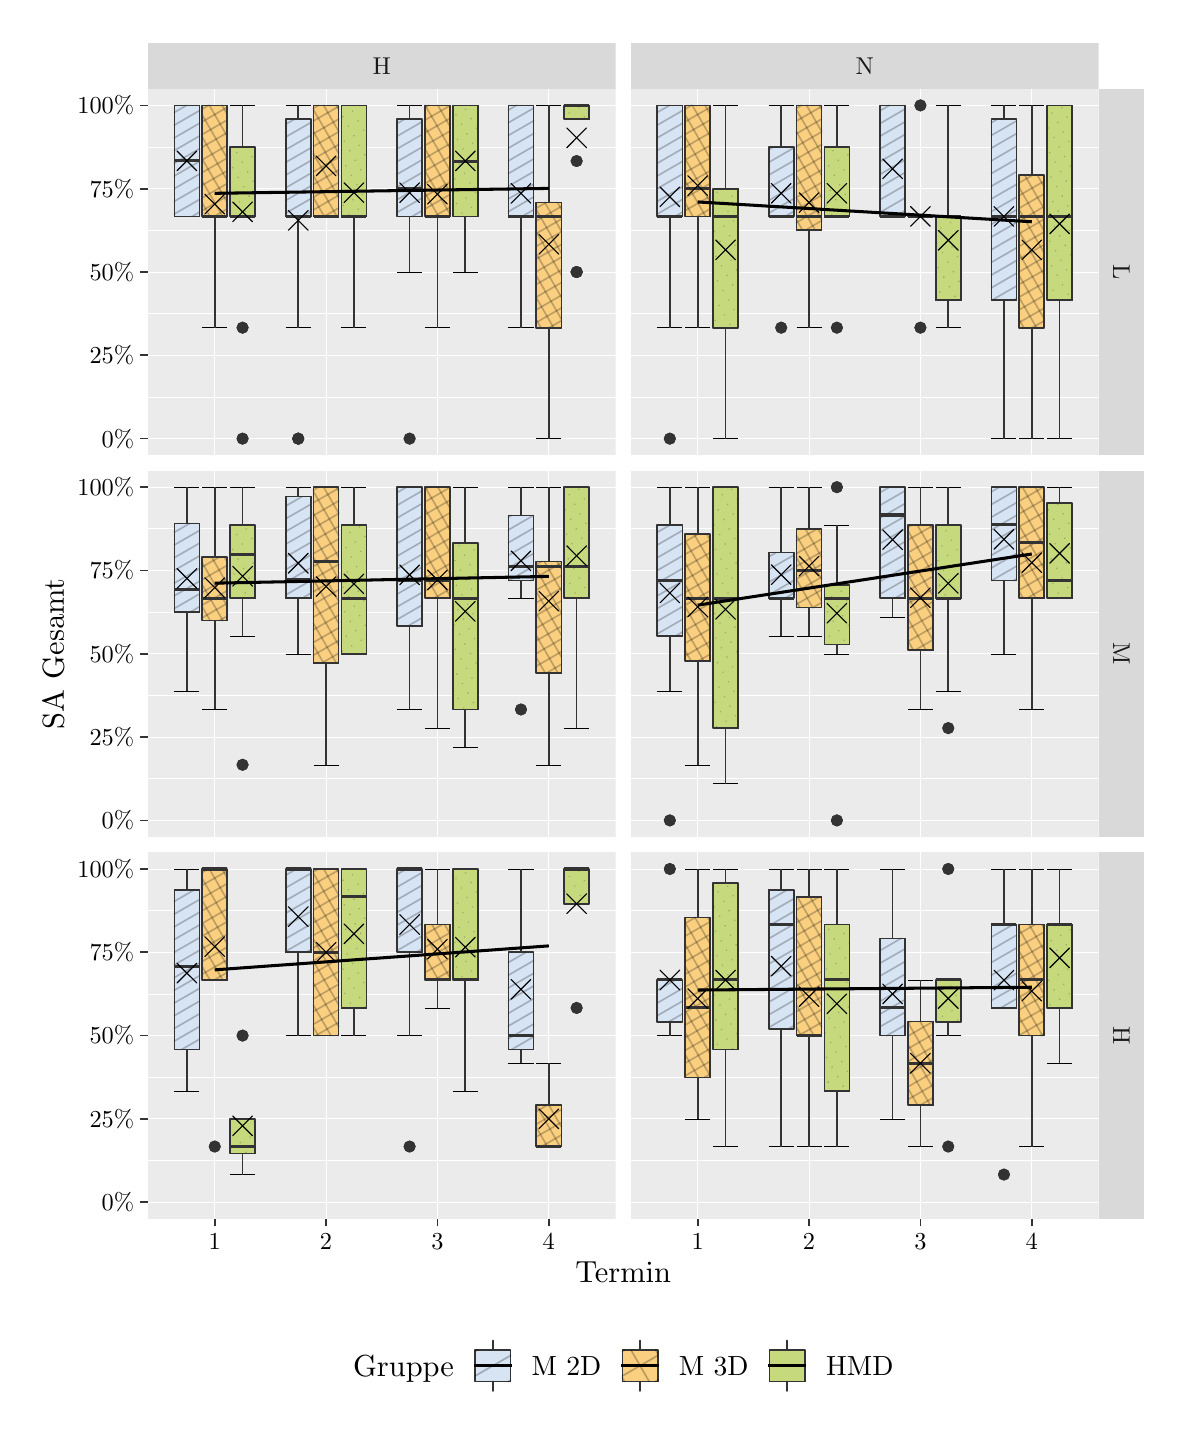
\begin{tikzpicture}[x=1pt,y=1pt]
\definecolor{fillColor}{RGB}{255,255,255}
\path[use as bounding box,fill=fillColor,fill opacity=0.00] (0,0) rectangle (409.05,505.89);
\begin{scope}
\path[clip] (  0.00,  0.00) rectangle (409.05,505.89);
\definecolor{drawColor}{RGB}{255,255,255}
\definecolor{fillColor}{RGB}{255,255,255}

\path[draw=drawColor,line width= 0.6pt,line join=round,line cap=round,fill=fillColor] (  0.00,  0.00) rectangle (409.05,505.89);
\end{scope}
\begin{scope}
\path[clip] ( 43.44,351.36) rectangle (212.46,483.82);
\definecolor{fillColor}{gray}{0.92}

\path[fill=fillColor] ( 43.44,351.36) rectangle (212.46,483.82);
\definecolor{drawColor}{RGB}{255,255,255}

\path[draw=drawColor,line width= 0.3pt,line join=round] ( 43.44,372.43) --
	(212.46,372.43);

\path[draw=drawColor,line width= 0.3pt,line join=round] ( 43.44,402.54) --
	(212.46,402.54);

\path[draw=drawColor,line width= 0.3pt,line join=round] ( 43.44,432.64) --
	(212.46,432.64);

\path[draw=drawColor,line width= 0.3pt,line join=round] ( 43.44,462.75) --
	(212.46,462.75);

\path[draw=drawColor,line width= 0.3pt,line join=round] ( 43.44,357.38) --
	(212.46,357.38);

\path[draw=drawColor,line width= 0.3pt,line join=round] ( 43.44,387.49) --
	(212.46,387.49);

\path[draw=drawColor,line width= 0.3pt,line join=round] ( 43.44,417.59) --
	(212.46,417.59);

\path[draw=drawColor,line width= 0.3pt,line join=round] ( 43.44,447.69) --
	(212.46,447.69);

\path[draw=drawColor,line width= 0.3pt,line join=round] ( 43.44,477.80) --
	(212.46,477.80);

\path[draw=drawColor,line width= 0.3pt,line join=round] ( 67.59,351.36) --
	( 67.59,483.82);

\path[draw=drawColor,line width= 0.3pt,line join=round] (107.83,351.36) --
	(107.83,483.82);

\path[draw=drawColor,line width= 0.3pt,line join=round] (148.07,351.36) --
	(148.07,483.82);

\path[draw=drawColor,line width= 0.3pt,line join=round] (188.31,351.36) --
	(188.31,483.82);
\definecolor{drawColor}{RGB}{0,0,0}

\path[draw=drawColor,line width= 0.2pt,line join=round] ( 53.00,477.80) --
	( 62.05,477.80);

\path[draw=drawColor,line width= 0.2pt,line join=round] ( 57.53,477.80) --
	( 57.53,437.70);

\path[draw=drawColor,line width= 0.2pt,line join=round] ( 53.00,437.70) --
	( 62.05,437.70);

\path[draw=drawColor,line width= 0.2pt,line join=round] ( 63.06,477.80) --
	( 72.12,477.80);

\path[draw=drawColor,line width= 0.2pt,line join=round] ( 67.59,477.80) --
	( 67.59,397.48);

\path[draw=drawColor,line width= 0.2pt,line join=round] ( 63.06,397.48) --
	( 72.12,397.48);

\path[draw=drawColor,line width= 0.2pt,line join=round] ( 73.12,477.80) --
	( 82.18,477.80);

\path[draw=drawColor,line width= 0.2pt,line join=round] ( 77.65,477.80) --
	( 77.65,437.70);

\path[draw=drawColor,line width= 0.2pt,line join=round] ( 73.12,437.70) --
	( 82.18,437.70);

\path[draw=drawColor,line width= 0.2pt,line join=round] ( 93.24,477.80) --
	(102.30,477.80);

\path[draw=drawColor,line width= 0.2pt,line join=round] ( 97.77,477.80) --
	( 97.77,397.48);

\path[draw=drawColor,line width= 0.2pt,line join=round] ( 93.24,397.48) --
	(102.30,397.48);

\path[draw=drawColor,line width= 0.2pt,line join=round] (103.30,477.80) --
	(112.36,477.80);

\path[draw=drawColor,line width= 0.2pt,line join=round] (107.83,477.80) --
	(107.83,437.70);

\path[draw=drawColor,line width= 0.2pt,line join=round] (103.30,437.70) --
	(112.36,437.70);

\path[draw=drawColor,line width= 0.2pt,line join=round] (113.36,477.80) --
	(122.42,477.80);

\path[draw=drawColor,line width= 0.2pt,line join=round] (117.89,477.80) --
	(117.89,397.48);

\path[draw=drawColor,line width= 0.2pt,line join=round] (113.36,397.48) --
	(122.42,397.48);

\path[draw=drawColor,line width= 0.2pt,line join=round] (133.48,477.80) --
	(142.54,477.80);

\path[draw=drawColor,line width= 0.2pt,line join=round] (138.01,477.80) --
	(138.01,417.59);

\path[draw=drawColor,line width= 0.2pt,line join=round] (133.48,417.59) --
	(142.54,417.59);

\path[draw=drawColor,line width= 0.2pt,line join=round] (143.55,477.80) --
	(152.60,477.80);

\path[draw=drawColor,line width= 0.2pt,line join=round] (148.07,477.80) --
	(148.07,397.48);

\path[draw=drawColor,line width= 0.2pt,line join=round] (143.55,397.48) --
	(152.60,397.48);

\path[draw=drawColor,line width= 0.2pt,line join=round] (153.61,477.80) --
	(162.66,477.80);

\path[draw=drawColor,line width= 0.2pt,line join=round] (158.13,477.80) --
	(158.13,417.59);

\path[draw=drawColor,line width= 0.2pt,line join=round] (153.61,417.59) --
	(162.66,417.59);

\path[draw=drawColor,line width= 0.2pt,line join=round] (173.73,477.80) --
	(182.78,477.80);

\path[draw=drawColor,line width= 0.2pt,line join=round] (178.25,477.80) --
	(178.25,397.48);

\path[draw=drawColor,line width= 0.2pt,line join=round] (173.73,397.48) --
	(182.78,397.48);

\path[draw=drawColor,line width= 0.2pt,line join=round] (183.79,477.80) --
	(192.84,477.80);

\path[draw=drawColor,line width= 0.2pt,line join=round] (188.31,477.80) --
	(188.31,357.38);

\path[draw=drawColor,line width= 0.2pt,line join=round] (183.79,357.38) --
	(192.84,357.38);

\path[draw=drawColor,line width= 0.2pt,line join=round] (193.85,477.80) --
	(202.90,477.80);

\path[draw=drawColor,line width= 0.2pt,line join=round] (198.37,477.80) --
	(198.37,472.77);

\path[draw=drawColor,line width= 0.2pt,line join=round] (193.85,472.77) --
	(202.90,472.77);
\definecolor{drawColor}{gray}{0.20}

\path[draw=drawColor,line width= 0.2pt,line join=round] ( 57.53,477.80) -- ( 57.53,477.80);

\path[draw=drawColor,line width= 0.2pt,line join=round] ( 57.53,437.70) -- ( 57.53,437.70);
\definecolor{fillColor}{RGB}{215,228,244}

\path[draw=drawColor,line width= 0.2pt,fill=fillColor] ( 53.00,477.80) --
	( 53.00,437.70) --
	( 62.05,437.70) --
	( 62.05,477.80) --
	( 53.00,477.80) --
	cycle;

\path[draw=drawColor,line width= 0.5pt] ( 53.00,457.75) -- ( 62.05,457.75);

\path[draw=drawColor,line width= 0.2pt,line join=round] ( 67.59,477.80) -- ( 67.59,477.80);

\path[draw=drawColor,line width= 0.2pt,line join=round] ( 67.59,437.70) -- ( 67.59,397.48);
\definecolor{fillColor}{RGB}{250,208,128}

\path[draw=drawColor,line width= 0.2pt,fill=fillColor] ( 63.06,477.80) --
	( 63.06,437.70) --
	( 72.12,437.70) --
	( 72.12,477.80) --
	( 63.06,477.80) --
	cycle;

\path[draw=drawColor,line width= 0.5pt] ( 63.06,437.70) -- ( 72.12,437.70);
\definecolor{fillColor}{gray}{0.20}

\path[draw=drawColor,line width= 0.4pt,line join=round,line cap=round,fill=fillColor] ( 77.65,357.38) circle (  1.96);

\path[draw=drawColor,line width= 0.4pt,line join=round,line cap=round,fill=fillColor] ( 77.65,397.48) circle (  1.96);

\path[draw=drawColor,line width= 0.2pt,line join=round] ( 77.65,462.72) -- ( 77.65,477.80);

\path[draw=drawColor,line width= 0.2pt,line join=round] ( 77.65,437.70) -- ( 77.65,437.70);
\definecolor{fillColor}{RGB}{199,217,125}

\path[draw=drawColor,line width= 0.2pt,fill=fillColor] ( 73.12,462.72) --
	( 73.12,437.70) --
	( 82.18,437.70) --
	( 82.18,462.72) --
	( 73.12,462.72) --
	cycle;

\path[draw=drawColor,line width= 0.5pt] ( 73.12,437.70) -- ( 82.18,437.70);
\definecolor{fillColor}{gray}{0.20}

\path[draw=drawColor,line width= 0.4pt,line join=round,line cap=round,fill=fillColor] ( 97.77,357.38) circle (  1.96);

\path[draw=drawColor,line width= 0.4pt,line join=round,line cap=round,fill=fillColor] ( 97.77,357.38) circle (  1.96);

\path[draw=drawColor,line width= 0.2pt,line join=round] ( 97.77,472.77) -- ( 97.77,477.80);

\path[draw=drawColor,line width= 0.2pt,line join=round] ( 97.77,437.70) -- ( 97.77,397.48);
\definecolor{fillColor}{RGB}{215,228,244}

\path[draw=drawColor,line width= 0.2pt,fill=fillColor] ( 93.24,472.77) --
	( 93.24,437.70) --
	(102.30,437.70) --
	(102.30,472.77) --
	( 93.24,472.77) --
	cycle;

\path[draw=drawColor,line width= 0.5pt] ( 93.24,437.70) -- (102.30,437.70);

\path[draw=drawColor,line width= 0.2pt,line join=round] (107.83,477.80) -- (107.83,477.80);

\path[draw=drawColor,line width= 0.2pt,line join=round] (107.83,437.70) -- (107.83,437.70);
\definecolor{fillColor}{RGB}{250,208,128}

\path[draw=drawColor,line width= 0.2pt,fill=fillColor] (103.30,477.80) --
	(103.30,437.70) --
	(112.36,437.70) --
	(112.36,477.80) --
	(103.30,477.80) --
	cycle;

\path[draw=drawColor,line width= 0.5pt] (103.30,437.70) -- (112.36,437.70);

\path[draw=drawColor,line width= 0.2pt,line join=round] (117.89,477.80) -- (117.89,477.80);

\path[draw=drawColor,line width= 0.2pt,line join=round] (117.89,437.70) -- (117.89,397.48);
\definecolor{fillColor}{RGB}{199,217,125}

\path[draw=drawColor,line width= 0.2pt,fill=fillColor] (113.36,477.80) --
	(113.36,437.70) --
	(122.42,437.70) --
	(122.42,477.80) --
	(113.36,477.80) --
	cycle;

\path[draw=drawColor,line width= 0.5pt] (113.36,437.70) -- (122.42,437.70);
\definecolor{fillColor}{gray}{0.20}

\path[draw=drawColor,line width= 0.4pt,line join=round,line cap=round,fill=fillColor] (138.01,357.38) circle (  1.96);

\path[draw=drawColor,line width= 0.2pt,line join=round] (138.01,472.77) -- (138.01,477.80);

\path[draw=drawColor,line width= 0.2pt,line join=round] (138.01,437.70) -- (138.01,417.59);
\definecolor{fillColor}{RGB}{215,228,244}

\path[draw=drawColor,line width= 0.2pt,fill=fillColor] (133.48,472.77) --
	(133.48,437.70) --
	(142.54,437.70) --
	(142.54,472.77) --
	(133.48,472.77) --
	cycle;

\path[draw=drawColor,line width= 0.5pt] (133.48,447.69) -- (142.54,447.69);

\path[draw=drawColor,line width= 0.2pt,line join=round] (148.07,477.80) -- (148.07,477.80);

\path[draw=drawColor,line width= 0.2pt,line join=round] (148.07,437.70) -- (148.07,397.48);
\definecolor{fillColor}{RGB}{250,208,128}

\path[draw=drawColor,line width= 0.2pt,fill=fillColor] (143.55,477.80) --
	(143.55,437.70) --
	(152.60,437.70) --
	(152.60,477.80) --
	(143.55,477.80) --
	cycle;

\path[draw=drawColor,line width= 0.5pt] (143.55,437.70) -- (152.60,437.70);

\path[draw=drawColor,line width= 0.2pt,line join=round] (158.13,477.80) -- (158.13,477.80);

\path[draw=drawColor,line width= 0.2pt,line join=round] (158.13,437.70) -- (158.13,417.59);
\definecolor{fillColor}{RGB}{199,217,125}

\path[draw=drawColor,line width= 0.2pt,fill=fillColor] (153.61,477.80) --
	(153.61,437.70) --
	(162.66,437.70) --
	(162.66,477.80) --
	(153.61,477.80) --
	cycle;

\path[draw=drawColor,line width= 0.5pt] (153.61,457.69) -- (162.66,457.69);

\path[draw=drawColor,line width= 0.2pt,line join=round] (178.25,477.80) -- (178.25,477.80);

\path[draw=drawColor,line width= 0.2pt,line join=round] (178.25,437.70) -- (178.25,397.48);
\definecolor{fillColor}{RGB}{215,228,244}

\path[draw=drawColor,line width= 0.2pt,fill=fillColor] (173.73,477.80) --
	(173.73,437.70) --
	(182.78,437.70) --
	(182.78,477.80) --
	(173.73,477.80) --
	cycle;

\path[draw=drawColor,line width= 0.5pt] (173.73,437.70) -- (182.78,437.70);

\path[draw=drawColor,line width= 0.2pt,line join=round] (188.31,442.70) -- (188.31,477.80);

\path[draw=drawColor,line width= 0.2pt,line join=round] (188.31,397.48) -- (188.31,357.38);
\definecolor{fillColor}{RGB}{250,208,128}

\path[draw=drawColor,line width= 0.2pt,fill=fillColor] (183.79,442.70) --
	(183.79,397.48) --
	(192.84,397.48) --
	(192.84,442.70) --
	(183.79,442.70) --
	cycle;

\path[draw=drawColor,line width= 0.5pt] (183.79,437.70) -- (192.84,437.70);
\definecolor{fillColor}{gray}{0.20}

\path[draw=drawColor,line width= 0.4pt,line join=round,line cap=round,fill=fillColor] (198.37,457.69) circle (  1.96);

\path[draw=drawColor,line width= 0.4pt,line join=round,line cap=round,fill=fillColor] (198.37,417.59) circle (  1.96);

\path[draw=drawColor,line width= 0.4pt,line join=round,line cap=round,fill=fillColor] (198.37,417.59) circle (  1.96);

\path[draw=drawColor,line width= 0.2pt,line join=round] (198.37,477.80) -- (198.37,477.80);

\path[draw=drawColor,line width= 0.2pt,line join=round] (198.37,472.77) -- (198.37,472.77);
\definecolor{fillColor}{RGB}{199,217,125}

\path[draw=drawColor,line width= 0.2pt,fill=fillColor] (193.85,477.80) --
	(193.85,472.77) --
	(202.90,472.77) --
	(202.90,477.80) --
	(193.85,477.80) --
	cycle;

\path[draw=drawColor,line width= 0.5pt] (193.85,477.80) -- (202.90,477.80);

\path[draw=drawColor,line width= 0.6pt,line join=round] ( 57.53,477.80) -- ( 57.53,477.80);

\path[draw=drawColor,line width= 0.6pt,line join=round] ( 57.53,437.70) -- ( 57.53,437.70);
\definecolor{fillColor}{RGB}{215,228,244}

\path[fill=fillColor] ( 53.00,477.80) --
	( 53.00,437.70) --
	( 62.05,437.70) --
	( 62.05,477.80) --
	( 53.00,477.80) --
	cycle;
\definecolor{drawColor}{RGB}{0,0,0}
\definecolor{fillColor}{RGB}{0,0,0}

\path[draw=drawColor,draw opacity=0.20,line width= 0.6pt,line join=round,line cap=rect,fill=fillColor,fill opacity=0.20] ( 62.05,439.22) --
	( 62.05,439.17) --
	( 59.51,437.70) --
	( 59.43,437.70) --
	( 62.05,439.22) --
	cycle;

\path[draw=drawColor,draw opacity=0.20,line width= 0.6pt,line join=round,line cap=rect,fill=fillColor,fill opacity=0.20] ( 62.05,443.81) --
	( 62.05,443.76) --
	( 53.00,438.53) --
	( 53.00,438.58) --
	( 62.05,443.81) --
	cycle;

\path[draw=drawColor,draw opacity=0.20,line width= 0.6pt,line join=round,line cap=rect,fill=fillColor,fill opacity=0.20] ( 62.05,448.39) --
	( 62.05,448.35) --
	( 53.00,443.12) --
	( 53.00,443.17) --
	( 62.05,448.39) --
	cycle;

\path[draw=drawColor,draw opacity=0.20,line width= 0.6pt,line join=round,line cap=rect,fill=fillColor,fill opacity=0.20] ( 62.05,452.98) --
	( 62.05,452.94) --
	( 53.00,447.71) --
	( 53.00,447.76) --
	( 62.05,452.98) --
	cycle;

\path[draw=drawColor,draw opacity=0.20,line width= 0.6pt,line join=round,line cap=rect,fill=fillColor,fill opacity=0.20] ( 62.05,457.57) --
	( 62.05,457.53) --
	( 53.00,452.30) --
	( 53.00,452.34) --
	( 62.05,457.57) --
	cycle;

\path[draw=drawColor,draw opacity=0.20,line width= 0.6pt,line join=round,line cap=rect,fill=fillColor,fill opacity=0.20] ( 62.05,462.16) --
	( 62.05,462.11) --
	( 53.00,456.89) --
	( 53.00,456.93) --
	( 62.05,462.16) --
	cycle;

\path[draw=drawColor,draw opacity=0.20,line width= 0.6pt,line join=round,line cap=rect,fill=fillColor,fill opacity=0.20] ( 62.05,466.75) --
	( 62.05,466.70) --
	( 53.00,461.47) --
	( 53.00,461.52) --
	( 62.05,466.75) --
	cycle;

\path[draw=drawColor,draw opacity=0.20,line width= 0.6pt,line join=round,line cap=rect,fill=fillColor,fill opacity=0.20] ( 62.05,471.34) --
	( 62.05,471.29) --
	( 53.00,466.06) --
	( 53.00,466.11) --
	( 62.05,471.34) --
	cycle;

\path[draw=drawColor,draw opacity=0.20,line width= 0.6pt,line join=round,line cap=rect,fill=fillColor,fill opacity=0.20] ( 62.05,475.92) --
	( 62.05,475.88) --
	( 53.00,470.65) --
	( 53.00,470.70) --
	( 62.05,475.92) --
	cycle;

\path[draw=drawColor,draw opacity=0.20,line width= 0.6pt,line join=round,line cap=rect,fill=fillColor,fill opacity=0.20] ( 57.35,477.80) --
	( 57.43,477.80) --
	( 53.00,475.24) --
	( 53.00,475.29) --
	( 57.35,477.80) --
	cycle;
\definecolor{drawColor}{gray}{0.20}

\path[draw=drawColor,line width= 0.6pt,line join=round,line cap=round] ( 53.00,477.80) --
	( 53.00,437.70) --
	( 62.05,437.70) --
	( 62.05,477.80) --
	( 53.00,477.80) --
	cycle;

\path[draw=drawColor,line width= 1.1pt,line join=round] ( 53.00,457.75) -- ( 62.05,457.75);
\definecolor{fillColor}{gray}{0.20}

\path[draw=drawColor,line width= 0.4pt,line join=round,line cap=round,fill=fillColor] ( 97.77,357.38) circle (  1.96);

\path[draw=drawColor,line width= 0.4pt,line join=round,line cap=round,fill=fillColor] ( 97.77,357.38) circle (  1.96);

\path[draw=drawColor,line width= 0.6pt,line join=round] ( 97.77,472.77) -- ( 97.77,477.80);

\path[draw=drawColor,line width= 0.6pt,line join=round] ( 97.77,437.70) -- ( 97.77,397.48);
\definecolor{fillColor}{RGB}{215,228,244}

\path[fill=fillColor] ( 93.24,472.77) --
	( 93.24,437.70) --
	(102.30,437.70) --
	(102.30,472.77) --
	( 93.24,472.77) --
	cycle;
\definecolor{drawColor}{RGB}{0,0,0}
\definecolor{fillColor}{RGB}{0,0,0}

\path[draw=drawColor,draw opacity=0.20,line width= 0.6pt,line join=round,line cap=rect,fill=fillColor,fill opacity=0.20] (102.30,439.51) --
	(102.30,439.46) --
	( 99.24,437.70) --
	( 99.16,437.70) --
	(102.30,439.51) --
	cycle;

\path[draw=drawColor,draw opacity=0.20,line width= 0.6pt,line join=round,line cap=rect,fill=fillColor,fill opacity=0.20] (102.30,444.10) --
	(102.30,444.05) --
	( 93.24,438.82) --
	( 93.24,438.87) --
	(102.30,444.10) --
	cycle;

\path[draw=drawColor,draw opacity=0.20,line width= 0.6pt,line join=round,line cap=rect,fill=fillColor,fill opacity=0.20] (102.30,448.69) --
	(102.30,448.64) --
	( 93.24,443.41) --
	( 93.24,443.46) --
	(102.30,448.69) --
	cycle;

\path[draw=drawColor,draw opacity=0.20,line width= 0.6pt,line join=round,line cap=rect,fill=fillColor,fill opacity=0.20] (102.30,453.27) --
	(102.30,453.23) --
	( 93.24,448.00) --
	( 93.24,448.05) --
	(102.30,453.27) --
	cycle;

\path[draw=drawColor,draw opacity=0.20,line width= 0.6pt,line join=round,line cap=rect,fill=fillColor,fill opacity=0.20] (102.30,457.86) --
	(102.30,457.82) --
	( 93.24,452.59) --
	( 93.24,452.64) --
	(102.30,457.86) --
	cycle;

\path[draw=drawColor,draw opacity=0.20,line width= 0.6pt,line join=round,line cap=rect,fill=fillColor,fill opacity=0.20] (102.30,462.45) --
	(102.30,462.41) --
	( 93.24,457.18) --
	( 93.24,457.22) --
	(102.30,462.45) --
	cycle;

\path[draw=drawColor,draw opacity=0.20,line width= 0.6pt,line join=round,line cap=rect,fill=fillColor,fill opacity=0.20] (102.30,467.04) --
	(102.30,466.99) --
	( 93.24,461.77) --
	( 93.24,461.81) --
	(102.30,467.04) --
	cycle;

\path[draw=drawColor,draw opacity=0.20,line width= 0.6pt,line join=round,line cap=rect,fill=fillColor,fill opacity=0.20] (102.30,471.63) --
	(102.30,471.58) --
	( 93.24,466.35) --
	( 93.24,466.40) --
	(102.30,471.63) --
	cycle;

\path[draw=drawColor,draw opacity=0.20,line width= 0.6pt,line join=round,line cap=rect,fill=fillColor,fill opacity=0.20] ( 96.33,472.77) --
	( 96.41,472.77) --
	( 93.24,470.94) --
	( 93.24,470.99) --
	( 96.33,472.77) --
	cycle;
\definecolor{drawColor}{gray}{0.20}

\path[draw=drawColor,line width= 0.6pt,line join=round,line cap=round] ( 93.24,472.77) --
	( 93.24,437.70) --
	(102.30,437.70) --
	(102.30,472.77) --
	( 93.24,472.77) --
	cycle;

\path[draw=drawColor,line width= 1.1pt,line join=round] ( 93.24,437.70) -- (102.30,437.70);
\definecolor{fillColor}{gray}{0.20}

\path[draw=drawColor,line width= 0.4pt,line join=round,line cap=round,fill=fillColor] (138.01,357.38) circle (  1.96);

\path[draw=drawColor,line width= 0.6pt,line join=round] (138.01,472.77) -- (138.01,477.80);

\path[draw=drawColor,line width= 0.6pt,line join=round] (138.01,437.70) -- (138.01,417.59);
\definecolor{fillColor}{RGB}{215,228,244}

\path[fill=fillColor] (133.48,472.77) --
	(133.48,437.70) --
	(142.54,437.70) --
	(142.54,472.77) --
	(133.48,472.77) --
	cycle;
\definecolor{drawColor}{RGB}{0,0,0}
\definecolor{fillColor}{RGB}{0,0,0}

\path[draw=drawColor,draw opacity=0.20,line width= 0.6pt,line join=round,line cap=rect,fill=fillColor,fill opacity=0.20] (142.54,439.80) --
	(142.54,439.75) --
	(138.98,437.70) --
	(138.90,437.70) --
	(142.54,439.80) --
	cycle;

\path[draw=drawColor,draw opacity=0.20,line width= 0.6pt,line join=round,line cap=rect,fill=fillColor,fill opacity=0.20] (142.54,444.39) --
	(142.54,444.34) --
	(133.48,439.12) --
	(133.48,439.16) --
	(142.54,444.39) --
	cycle;

\path[draw=drawColor,draw opacity=0.20,line width= 0.6pt,line join=round,line cap=rect,fill=fillColor,fill opacity=0.20] (142.54,448.98) --
	(142.54,448.93) --
	(133.48,443.70) --
	(133.48,443.75) --
	(142.54,448.98) --
	cycle;

\path[draw=drawColor,draw opacity=0.20,line width= 0.6pt,line join=round,line cap=rect,fill=fillColor,fill opacity=0.20] (142.54,453.57) --
	(142.54,453.52) --
	(133.48,448.29) --
	(133.48,448.34) --
	(142.54,453.57) --
	cycle;

\path[draw=drawColor,draw opacity=0.20,line width= 0.6pt,line join=round,line cap=rect,fill=fillColor,fill opacity=0.20] (142.54,458.15) --
	(142.54,458.11) --
	(133.48,452.88) --
	(133.48,452.93) --
	(142.54,458.15) --
	cycle;

\path[draw=drawColor,draw opacity=0.20,line width= 0.6pt,line join=round,line cap=rect,fill=fillColor,fill opacity=0.20] (142.54,462.74) --
	(142.54,462.70) --
	(133.48,457.47) --
	(133.48,457.52) --
	(142.54,462.74) --
	cycle;

\path[draw=drawColor,draw opacity=0.20,line width= 0.6pt,line join=round,line cap=rect,fill=fillColor,fill opacity=0.20] (142.54,467.33) --
	(142.54,467.29) --
	(133.48,462.06) --
	(133.48,462.10) --
	(142.54,467.33) --
	cycle;

\path[draw=drawColor,draw opacity=0.20,line width= 0.6pt,line join=round,line cap=rect,fill=fillColor,fill opacity=0.20] (142.54,471.92) --
	(142.54,471.87) --
	(133.48,466.65) --
	(133.48,466.69) --
	(142.54,471.92) --
	cycle;

\path[draw=drawColor,draw opacity=0.20,line width= 0.6pt,line join=round,line cap=rect,fill=fillColor,fill opacity=0.20] (136.07,472.77) --
	(136.14,472.77) --
	(133.48,471.23) --
	(133.48,471.28) --
	(136.07,472.77) --
	cycle;
\definecolor{drawColor}{gray}{0.20}

\path[draw=drawColor,line width= 0.6pt,line join=round,line cap=round] (133.48,472.77) --
	(133.48,437.70) --
	(142.54,437.70) --
	(142.54,472.77) --
	(133.48,472.77) --
	cycle;

\path[draw=drawColor,line width= 1.1pt,line join=round] (133.48,447.69) -- (142.54,447.69);

\path[draw=drawColor,line width= 0.6pt,line join=round] (178.25,477.80) -- (178.25,477.80);

\path[draw=drawColor,line width= 0.6pt,line join=round] (178.25,437.70) -- (178.25,397.48);
\definecolor{fillColor}{RGB}{215,228,244}

\path[fill=fillColor] (173.73,477.80) --
	(173.73,437.70) --
	(182.78,437.70) --
	(182.78,477.80) --
	(173.73,477.80) --
	cycle;
\definecolor{drawColor}{RGB}{0,0,0}
\definecolor{fillColor}{RGB}{0,0,0}

\path[draw=drawColor,draw opacity=0.20,line width= 0.6pt,line join=round,line cap=rect,fill=fillColor,fill opacity=0.20] (182.78,440.09) --
	(182.78,440.05) --
	(178.72,437.70) --
	(178.64,437.70) --
	(182.78,440.09) --
	cycle;

\path[draw=drawColor,draw opacity=0.20,line width= 0.6pt,line join=round,line cap=rect,fill=fillColor,fill opacity=0.20] (182.78,444.68) --
	(182.78,444.63) --
	(173.73,439.41) --
	(173.73,439.45) --
	(182.78,444.68) --
	cycle;

\path[draw=drawColor,draw opacity=0.20,line width= 0.6pt,line join=round,line cap=rect,fill=fillColor,fill opacity=0.20] (182.78,449.27) --
	(182.78,449.22) --
	(173.73,444.00) --
	(173.73,444.04) --
	(182.78,449.27) --
	cycle;

\path[draw=drawColor,draw opacity=0.20,line width= 0.6pt,line join=round,line cap=rect,fill=fillColor,fill opacity=0.20] (182.78,453.86) --
	(182.78,453.81) --
	(173.73,448.58) --
	(173.73,448.63) --
	(182.78,453.86) --
	cycle;

\path[draw=drawColor,draw opacity=0.20,line width= 0.6pt,line join=round,line cap=rect,fill=fillColor,fill opacity=0.20] (182.78,458.45) --
	(182.78,458.40) --
	(173.73,453.17) --
	(173.73,453.22) --
	(182.78,458.45) --
	cycle;

\path[draw=drawColor,draw opacity=0.20,line width= 0.6pt,line join=round,line cap=rect,fill=fillColor,fill opacity=0.20] (182.78,463.03) --
	(182.78,462.99) --
	(173.73,457.76) --
	(173.73,457.81) --
	(182.78,463.03) --
	cycle;

\path[draw=drawColor,draw opacity=0.20,line width= 0.6pt,line join=round,line cap=rect,fill=fillColor,fill opacity=0.20] (182.78,467.62) --
	(182.78,467.58) --
	(173.73,462.35) --
	(173.73,462.40) --
	(182.78,467.62) --
	cycle;

\path[draw=drawColor,draw opacity=0.20,line width= 0.6pt,line join=round,line cap=rect,fill=fillColor,fill opacity=0.20] (182.78,472.21) --
	(182.78,472.17) --
	(173.73,466.94) --
	(173.73,466.98) --
	(182.78,472.21) --
	cycle;

\path[draw=drawColor,draw opacity=0.20,line width= 0.6pt,line join=round,line cap=rect,fill=fillColor,fill opacity=0.20] (182.78,476.80) --
	(182.78,476.75) --
	(173.73,471.53) --
	(173.73,471.57) --
	(182.78,476.80) --
	cycle;

\path[draw=drawColor,draw opacity=0.20,line width= 0.6pt,line join=round,line cap=rect,fill=fillColor,fill opacity=0.20] (176.56,477.80) --
	(176.64,477.80) --
	(173.73,476.11) --
	(173.73,476.16) --
	(176.56,477.80) --
	cycle;
\definecolor{drawColor}{gray}{0.20}

\path[draw=drawColor,line width= 0.6pt,line join=round,line cap=round] (173.73,477.80) --
	(173.73,437.70) --
	(182.78,437.70) --
	(182.78,477.80) --
	(173.73,477.80) --
	cycle;

\path[draw=drawColor,line width= 1.1pt,line join=round] (173.73,437.70) -- (182.78,437.70);

\path[draw=drawColor,line width= 0.6pt,line join=round] ( 67.59,477.80) -- ( 67.59,477.80);

\path[draw=drawColor,line width= 0.6pt,line join=round] ( 67.59,437.70) -- ( 67.59,397.48);
\definecolor{fillColor}{RGB}{250,208,128}

\path[fill=fillColor] ( 63.06,477.80) --
	( 63.06,437.70) --
	( 72.12,437.70) --
	( 72.12,477.80) --
	( 63.06,477.80) --
	cycle;
\definecolor{drawColor}{RGB}{0,0,0}
\definecolor{fillColor}{RGB}{0,0,0}

\path[draw=drawColor,draw opacity=0.20,line width= 0.6pt,line join=round,line cap=rect,fill=fillColor,fill opacity=0.20] ( 72.12,440.44) --
	( 72.12,440.39) --
	( 67.45,437.70) --
	( 67.37,437.70) --
	( 72.12,440.44) --
	cycle;

\path[draw=drawColor,draw opacity=0.20,line width= 0.6pt,line join=round,line cap=rect,fill=fillColor,fill opacity=0.20] ( 72.12,445.03) --
	( 72.12,444.98) --
	( 63.06,439.75) --
	( 63.06,439.80) --
	( 72.12,445.03) --
	cycle;

\path[draw=drawColor,draw opacity=0.20,line width= 0.6pt,line join=round,line cap=rect,fill=fillColor,fill opacity=0.20] ( 72.12,449.61) --
	( 72.12,449.57) --
	( 63.06,444.34) --
	( 63.06,444.39) --
	( 72.12,449.61) --
	cycle;

\path[draw=drawColor,draw opacity=0.20,line width= 0.6pt,line join=round,line cap=rect,fill=fillColor,fill opacity=0.20] ( 72.12,454.20) --
	( 72.12,454.16) --
	( 63.06,448.93) --
	( 63.06,448.98) --
	( 72.12,454.20) --
	cycle;

\path[draw=drawColor,draw opacity=0.20,line width= 0.6pt,line join=round,line cap=rect,fill=fillColor,fill opacity=0.20] ( 72.12,458.79) --
	( 72.12,458.75) --
	( 63.06,453.52) --
	( 63.06,453.56) --
	( 72.12,458.79) --
	cycle;

\path[draw=drawColor,draw opacity=0.20,line width= 0.6pt,line join=round,line cap=rect,fill=fillColor,fill opacity=0.20] ( 72.12,463.38) --
	( 72.12,463.33) --
	( 63.06,458.11) --
	( 63.06,458.15) --
	( 72.12,463.38) --
	cycle;

\path[draw=drawColor,draw opacity=0.20,line width= 0.6pt,line join=round,line cap=rect,fill=fillColor,fill opacity=0.20] ( 72.12,467.97) --
	( 72.12,467.92) --
	( 63.06,462.69) --
	( 63.06,462.74) --
	( 72.12,467.97) --
	cycle;

\path[draw=drawColor,draw opacity=0.20,line width= 0.6pt,line join=round,line cap=rect,fill=fillColor,fill opacity=0.20] ( 72.12,472.56) --
	( 72.12,472.51) --
	( 63.06,467.28) --
	( 63.06,467.33) --
	( 72.12,472.56) --
	cycle;

\path[draw=drawColor,draw opacity=0.20,line width= 0.6pt,line join=round,line cap=rect,fill=fillColor,fill opacity=0.20] ( 72.12,477.14) --
	( 72.12,477.10) --
	( 63.06,471.87) --
	( 63.06,471.92) --
	( 72.12,477.14) --
	cycle;

\path[draw=drawColor,draw opacity=0.20,line width= 0.6pt,line join=round,line cap=rect,fill=fillColor,fill opacity=0.20] ( 65.30,477.80) --
	( 65.38,477.80) --
	( 63.06,476.46) --
	( 63.06,476.51) --
	( 65.30,477.80) --
	cycle;

\path[draw=drawColor,draw opacity=0.20,line width= 0.6pt,line join=round,line cap=rect,fill=fillColor,fill opacity=0.20] ( 65.89,437.70) --
	( 65.85,437.70) --
	( 63.06,442.52) --
	( 63.06,442.60) --
	( 65.89,437.70) --
	cycle;

\path[draw=drawColor,draw opacity=0.20,line width= 0.6pt,line join=round,line cap=rect,fill=fillColor,fill opacity=0.20] ( 70.48,437.70) --
	( 70.43,437.70) --
	( 63.06,450.47) --
	( 63.06,450.55) --
	( 70.48,437.70) --
	cycle;

\path[draw=drawColor,draw opacity=0.20,line width= 0.6pt,line join=round,line cap=rect,fill=fillColor,fill opacity=0.20] ( 72.12,442.81) --
	( 72.12,442.73) --
	( 63.06,458.42) --
	( 63.06,458.50) --
	( 72.12,442.81) --
	cycle;

\path[draw=drawColor,draw opacity=0.20,line width= 0.6pt,line join=round,line cap=rect,fill=fillColor,fill opacity=0.20] ( 72.12,450.76) --
	( 72.12,450.68) --
	( 63.06,466.36) --
	( 63.06,466.44) --
	( 72.12,450.76) --
	cycle;

\path[draw=drawColor,draw opacity=0.20,line width= 0.6pt,line join=round,line cap=rect,fill=fillColor,fill opacity=0.20] ( 72.12,458.71) --
	( 72.12,458.63) --
	( 63.06,474.31) --
	( 63.06,474.39) --
	( 72.12,458.71) --
	cycle;

\path[draw=drawColor,draw opacity=0.20,line width= 0.6pt,line join=round,line cap=rect,fill=fillColor,fill opacity=0.20] ( 72.12,466.66) --
	( 72.12,466.58) --
	( 65.64,477.80) --
	( 65.68,477.80) --
	( 72.12,466.66) --
	cycle;

\path[draw=drawColor,draw opacity=0.20,line width= 0.6pt,line join=round,line cap=rect,fill=fillColor,fill opacity=0.20] ( 72.12,474.60) --
	( 72.12,474.52) --
	( 70.23,477.80) --
	( 70.27,477.80) --
	( 72.12,474.60) --
	cycle;
\definecolor{drawColor}{gray}{0.20}

\path[draw=drawColor,line width= 0.6pt,line join=round,line cap=round] ( 63.06,477.80) --
	( 63.06,437.70) --
	( 72.12,437.70) --
	( 72.12,477.80) --
	( 63.06,477.80) --
	cycle;

\path[draw=drawColor,line width= 1.1pt,line join=round] ( 63.06,437.70) -- ( 72.12,437.70);

\path[draw=drawColor,line width= 0.6pt,line join=round] (107.83,477.80) -- (107.83,477.80);

\path[draw=drawColor,line width= 0.6pt,line join=round] (107.83,437.70) -- (107.83,437.70);
\definecolor{fillColor}{RGB}{250,208,128}

\path[fill=fillColor] (103.30,477.80) --
	(103.30,437.70) --
	(112.36,437.70) --
	(112.36,477.80) --
	(103.30,477.80) --
	cycle;
\definecolor{drawColor}{RGB}{0,0,0}
\definecolor{fillColor}{RGB}{0,0,0}

\path[draw=drawColor,draw opacity=0.20,line width= 0.6pt,line join=round,line cap=rect,fill=fillColor,fill opacity=0.20] (112.36,440.73) --
	(112.36,440.68) --
	(107.19,437.70) --
	(107.11,437.70) --
	(112.36,440.73) --
	cycle;

\path[draw=drawColor,draw opacity=0.20,line width= 0.6pt,line join=round,line cap=rect,fill=fillColor,fill opacity=0.20] (112.36,445.32) --
	(112.36,445.27) --
	(103.30,440.04) --
	(103.30,440.09) --
	(112.36,445.32) --
	cycle;

\path[draw=drawColor,draw opacity=0.20,line width= 0.6pt,line join=round,line cap=rect,fill=fillColor,fill opacity=0.20] (112.36,449.91) --
	(112.36,449.86) --
	(103.30,444.63) --
	(103.30,444.68) --
	(112.36,449.91) --
	cycle;

\path[draw=drawColor,draw opacity=0.20,line width= 0.6pt,line join=round,line cap=rect,fill=fillColor,fill opacity=0.20] (112.36,454.49) --
	(112.36,454.45) --
	(103.30,449.22) --
	(103.30,449.27) --
	(112.36,454.49) --
	cycle;

\path[draw=drawColor,draw opacity=0.20,line width= 0.6pt,line join=round,line cap=rect,fill=fillColor,fill opacity=0.20] (112.36,459.08) --
	(112.36,459.04) --
	(103.30,453.81) --
	(103.30,453.86) --
	(112.36,459.08) --
	cycle;

\path[draw=drawColor,draw opacity=0.20,line width= 0.6pt,line join=round,line cap=rect,fill=fillColor,fill opacity=0.20] (112.36,463.67) --
	(112.36,463.63) --
	(103.30,458.40) --
	(103.30,458.44) --
	(112.36,463.67) --
	cycle;

\path[draw=drawColor,draw opacity=0.20,line width= 0.6pt,line join=round,line cap=rect,fill=fillColor,fill opacity=0.20] (112.36,468.26) --
	(112.36,468.21) --
	(103.30,462.99) --
	(103.30,463.03) --
	(112.36,468.26) --
	cycle;

\path[draw=drawColor,draw opacity=0.20,line width= 0.6pt,line join=round,line cap=rect,fill=fillColor,fill opacity=0.20] (112.36,472.85) --
	(112.36,472.80) --
	(103.30,467.57) --
	(103.30,467.62) --
	(112.36,472.85) --
	cycle;

\path[draw=drawColor,draw opacity=0.20,line width= 0.6pt,line join=round,line cap=rect,fill=fillColor,fill opacity=0.20] (112.36,477.44) --
	(112.36,477.39) --
	(103.30,472.16) --
	(103.30,472.21) --
	(112.36,477.44) --
	cycle;

\path[draw=drawColor,draw opacity=0.20,line width= 0.6pt,line join=round,line cap=rect,fill=fillColor,fill opacity=0.20] (105.04,477.80) --
	(105.12,477.80) --
	(103.30,476.75) --
	(103.30,476.80) --
	(105.04,477.80) --
	cycle;

\path[draw=drawColor,draw opacity=0.20,line width= 0.6pt,line join=round,line cap=rect,fill=fillColor,fill opacity=0.20] (107.19,437.70) --
	(107.14,437.70) --
	(103.30,444.35) --
	(103.30,444.43) --
	(107.19,437.70) --
	cycle;

\path[draw=drawColor,draw opacity=0.20,line width= 0.6pt,line join=round,line cap=rect,fill=fillColor,fill opacity=0.20] (111.78,437.70) --
	(111.73,437.70) --
	(103.30,452.30) --
	(103.30,452.37) --
	(111.78,437.70) --
	cycle;

\path[draw=drawColor,draw opacity=0.20,line width= 0.6pt,line join=round,line cap=rect,fill=fillColor,fill opacity=0.20] (112.36,444.64) --
	(112.36,444.56) --
	(103.30,460.24) --
	(103.30,460.32) --
	(112.36,444.64) --
	cycle;

\path[draw=drawColor,draw opacity=0.20,line width= 0.6pt,line join=round,line cap=rect,fill=fillColor,fill opacity=0.20] (112.36,452.59) --
	(112.36,452.51) --
	(103.30,468.19) --
	(103.30,468.27) --
	(112.36,452.59) --
	cycle;

\path[draw=drawColor,draw opacity=0.20,line width= 0.6pt,line join=round,line cap=rect,fill=fillColor,fill opacity=0.20] (112.36,460.53) --
	(112.36,460.45) --
	(103.30,476.14) --
	(103.30,476.22) --
	(112.36,460.53) --
	cycle;

\path[draw=drawColor,draw opacity=0.20,line width= 0.6pt,line join=round,line cap=rect,fill=fillColor,fill opacity=0.20] (112.36,468.48) --
	(112.36,468.40) --
	(106.93,477.80) --
	(106.98,477.80) --
	(112.36,468.48) --
	cycle;

\path[draw=drawColor,draw opacity=0.20,line width= 0.6pt,line join=round,line cap=rect,fill=fillColor,fill opacity=0.20] (112.36,476.43) --
	(112.36,476.35) --
	(111.52,477.80) --
	(111.57,477.80) --
	(112.36,476.43) --
	cycle;
\definecolor{drawColor}{gray}{0.20}

\path[draw=drawColor,line width= 0.6pt,line join=round,line cap=round] (103.30,477.80) --
	(103.30,437.70) --
	(112.36,437.70) --
	(112.36,477.80) --
	(103.30,477.80) --
	cycle;

\path[draw=drawColor,line width= 1.1pt,line join=round] (103.30,437.70) -- (112.36,437.70);

\path[draw=drawColor,line width= 0.6pt,line join=round] (148.07,477.80) -- (148.07,477.80);

\path[draw=drawColor,line width= 0.6pt,line join=round] (148.07,437.70) -- (148.07,397.48);
\definecolor{fillColor}{RGB}{250,208,128}

\path[fill=fillColor] (143.55,477.80) --
	(143.55,437.70) --
	(152.60,437.70) --
	(152.60,477.80) --
	(143.55,477.80) --
	cycle;
\definecolor{drawColor}{RGB}{0,0,0}
\definecolor{fillColor}{RGB}{0,0,0}

\path[draw=drawColor,draw opacity=0.20,line width= 0.6pt,line join=round,line cap=rect,fill=fillColor,fill opacity=0.20] (152.60,441.02) --
	(152.60,440.97) --
	(146.93,437.70) --
	(146.85,437.70) --
	(152.60,441.02) --
	cycle;

\path[draw=drawColor,draw opacity=0.20,line width= 0.6pt,line join=round,line cap=rect,fill=fillColor,fill opacity=0.20] (152.60,445.61) --
	(152.60,445.56) --
	(143.55,440.34) --
	(143.55,440.38) --
	(152.60,445.61) --
	cycle;

\path[draw=drawColor,draw opacity=0.20,line width= 0.6pt,line join=round,line cap=rect,fill=fillColor,fill opacity=0.20] (152.60,450.20) --
	(152.60,450.15) --
	(143.55,444.92) --
	(143.55,444.97) --
	(152.60,450.20) --
	cycle;

\path[draw=drawColor,draw opacity=0.20,line width= 0.6pt,line join=round,line cap=rect,fill=fillColor,fill opacity=0.20] (152.60,454.79) --
	(152.60,454.74) --
	(143.55,449.51) --
	(143.55,449.56) --
	(152.60,454.79) --
	cycle;

\path[draw=drawColor,draw opacity=0.20,line width= 0.6pt,line join=round,line cap=rect,fill=fillColor,fill opacity=0.20] (152.60,459.37) --
	(152.60,459.33) --
	(143.55,454.10) --
	(143.55,454.15) --
	(152.60,459.37) --
	cycle;

\path[draw=drawColor,draw opacity=0.20,line width= 0.6pt,line join=round,line cap=rect,fill=fillColor,fill opacity=0.20] (152.60,463.96) --
	(152.60,463.92) --
	(143.55,458.69) --
	(143.55,458.74) --
	(152.60,463.96) --
	cycle;

\path[draw=drawColor,draw opacity=0.20,line width= 0.6pt,line join=round,line cap=rect,fill=fillColor,fill opacity=0.20] (152.60,468.55) --
	(152.60,468.51) --
	(143.55,463.28) --
	(143.55,463.32) --
	(152.60,468.55) --
	cycle;

\path[draw=drawColor,draw opacity=0.20,line width= 0.6pt,line join=round,line cap=rect,fill=fillColor,fill opacity=0.20] (152.60,473.14) --
	(152.60,473.09) --
	(143.55,467.87) --
	(143.55,467.91) --
	(152.60,473.14) --
	cycle;

\path[draw=drawColor,draw opacity=0.20,line width= 0.6pt,line join=round,line cap=rect,fill=fillColor,fill opacity=0.20] (152.60,477.73) --
	(152.60,477.68) --
	(143.55,472.45) --
	(143.55,472.50) --
	(152.60,477.73) --
	cycle;

\path[draw=drawColor,draw opacity=0.20,line width= 0.6pt,line join=round,line cap=rect,fill=fillColor,fill opacity=0.20] (144.77,477.80) --
	(144.85,477.80) --
	(143.55,477.04) --
	(143.55,477.09) --
	(144.77,477.80) --
	cycle;

\path[draw=drawColor,draw opacity=0.20,line width= 0.6pt,line join=round,line cap=rect,fill=fillColor,fill opacity=0.20] (143.89,437.70) --
	(143.85,437.70) --
	(143.55,438.23) --
	(143.55,438.30) --
	(143.89,437.70) --
	cycle;

\path[draw=drawColor,draw opacity=0.20,line width= 0.6pt,line join=round,line cap=rect,fill=fillColor,fill opacity=0.20] (148.48,437.70) --
	(148.44,437.70) --
	(143.55,446.17) --
	(143.55,446.25) --
	(148.48,437.70) --
	cycle;

\path[draw=drawColor,draw opacity=0.20,line width= 0.6pt,line join=round,line cap=rect,fill=fillColor,fill opacity=0.20] (152.60,438.52) --
	(152.60,438.44) --
	(143.55,454.12) --
	(143.55,454.20) --
	(152.60,438.52) --
	cycle;

\path[draw=drawColor,draw opacity=0.20,line width= 0.6pt,line join=round,line cap=rect,fill=fillColor,fill opacity=0.20] (152.60,446.46) --
	(152.60,446.38) --
	(143.55,462.07) --
	(143.55,462.15) --
	(152.60,446.46) --
	cycle;

\path[draw=drawColor,draw opacity=0.20,line width= 0.6pt,line join=round,line cap=rect,fill=fillColor,fill opacity=0.20] (152.60,454.41) --
	(152.60,454.33) --
	(143.55,470.02) --
	(143.55,470.09) --
	(152.60,454.41) --
	cycle;

\path[draw=drawColor,draw opacity=0.20,line width= 0.6pt,line join=round,line cap=rect,fill=fillColor,fill opacity=0.20] (152.60,462.36) --
	(152.60,462.28) --
	(143.64,477.80) --
	(143.69,477.80) --
	(152.60,462.36) --
	cycle;

\path[draw=drawColor,draw opacity=0.20,line width= 0.6pt,line join=round,line cap=rect,fill=fillColor,fill opacity=0.20] (152.60,470.31) --
	(152.60,470.23) --
	(148.23,477.80) --
	(148.27,477.80) --
	(152.60,470.31) --
	cycle;
\definecolor{drawColor}{gray}{0.20}

\path[draw=drawColor,line width= 0.6pt,line join=round,line cap=round] (143.55,477.80) --
	(143.55,437.70) --
	(152.60,437.70) --
	(152.60,477.80) --
	(143.55,477.80) --
	cycle;

\path[draw=drawColor,line width= 1.1pt,line join=round] (143.55,437.70) -- (152.60,437.70);

\path[draw=drawColor,line width= 0.6pt,line join=round] (188.31,442.70) -- (188.31,477.80);

\path[draw=drawColor,line width= 0.6pt,line join=round] (188.31,397.48) -- (188.31,357.38);
\definecolor{fillColor}{RGB}{250,208,128}

\path[fill=fillColor] (183.79,442.70) --
	(183.79,397.48) --
	(192.84,397.48) --
	(192.84,442.70) --
	(183.79,442.70) --
	cycle;
\definecolor{drawColor}{RGB}{0,0,0}
\definecolor{fillColor}{RGB}{0,0,0}

\path[draw=drawColor,draw opacity=0.20,line width= 0.6pt,line join=round,line cap=rect,fill=fillColor,fill opacity=0.20] (192.84,400.02) --
	(192.84,399.97) --
	(188.53,397.48) --
	(188.45,397.48) --
	(192.84,400.02) --
	cycle;

\path[draw=drawColor,draw opacity=0.20,line width= 0.6pt,line join=round,line cap=rect,fill=fillColor,fill opacity=0.20] (192.84,404.60) --
	(192.84,404.56) --
	(183.79,399.33) --
	(183.79,399.38) --
	(192.84,404.60) --
	cycle;

\path[draw=drawColor,draw opacity=0.20,line width= 0.6pt,line join=round,line cap=rect,fill=fillColor,fill opacity=0.20] (192.84,409.19) --
	(192.84,409.15) --
	(183.79,403.92) --
	(183.79,403.97) --
	(192.84,409.19) --
	cycle;

\path[draw=drawColor,draw opacity=0.20,line width= 0.6pt,line join=round,line cap=rect,fill=fillColor,fill opacity=0.20] (192.84,413.78) --
	(192.84,413.74) --
	(183.79,408.51) --
	(183.79,408.55) --
	(192.84,413.78) --
	cycle;

\path[draw=drawColor,draw opacity=0.20,line width= 0.6pt,line join=round,line cap=rect,fill=fillColor,fill opacity=0.20] (192.84,418.37) --
	(192.84,418.32) --
	(183.79,413.10) --
	(183.79,413.14) --
	(192.84,418.37) --
	cycle;

\path[draw=drawColor,draw opacity=0.20,line width= 0.6pt,line join=round,line cap=rect,fill=fillColor,fill opacity=0.20] (192.84,422.96) --
	(192.84,422.91) --
	(183.79,417.68) --
	(183.79,417.73) --
	(192.84,422.96) --
	cycle;

\path[draw=drawColor,draw opacity=0.20,line width= 0.6pt,line join=round,line cap=rect,fill=fillColor,fill opacity=0.20] (192.84,427.55) --
	(192.84,427.50) --
	(183.79,422.27) --
	(183.79,422.32) --
	(192.84,427.55) --
	cycle;

\path[draw=drawColor,draw opacity=0.20,line width= 0.6pt,line join=round,line cap=rect,fill=fillColor,fill opacity=0.20] (192.84,432.14) --
	(192.84,432.09) --
	(183.79,426.86) --
	(183.79,426.91) --
	(192.84,432.14) --
	cycle;

\path[draw=drawColor,draw opacity=0.20,line width= 0.6pt,line join=round,line cap=rect,fill=fillColor,fill opacity=0.20] (192.84,436.72) --
	(192.84,436.68) --
	(183.79,431.45) --
	(183.79,431.50) --
	(192.84,436.72) --
	cycle;

\path[draw=drawColor,draw opacity=0.20,line width= 0.6pt,line join=round,line cap=rect,fill=fillColor,fill opacity=0.20] (192.84,441.31) --
	(192.84,441.27) --
	(183.79,436.04) --
	(183.79,436.08) --
	(192.84,441.31) --
	cycle;

\path[draw=drawColor,draw opacity=0.20,line width= 0.6pt,line join=round,line cap=rect,fill=fillColor,fill opacity=0.20] (187.29,442.70) --
	(187.37,442.70) --
	(183.79,440.63) --
	(183.79,440.67) --
	(187.29,442.70) --
	cycle;

\path[draw=drawColor,draw opacity=0.20,line width= 0.6pt,line join=round,line cap=rect,fill=fillColor,fill opacity=0.20] (185.47,397.48) --
	(185.42,397.48) --
	(183.79,400.31) --
	(183.79,400.39) --
	(185.47,397.48) --
	cycle;

\path[draw=drawColor,draw opacity=0.20,line width= 0.6pt,line join=round,line cap=rect,fill=fillColor,fill opacity=0.20] (190.06,397.48) --
	(190.01,397.48) --
	(183.79,408.26) --
	(183.79,408.34) --
	(190.06,397.48) --
	cycle;

\path[draw=drawColor,draw opacity=0.20,line width= 0.6pt,line join=round,line cap=rect,fill=fillColor,fill opacity=0.20] (192.84,400.61) --
	(192.84,400.53) --
	(183.79,416.21) --
	(183.79,416.29) --
	(192.84,400.61) --
	cycle;

\path[draw=drawColor,draw opacity=0.20,line width= 0.6pt,line join=round,line cap=rect,fill=fillColor,fill opacity=0.20] (192.84,408.55) --
	(192.84,408.47) --
	(183.79,424.16) --
	(183.79,424.24) --
	(192.84,408.55) --
	cycle;

\path[draw=drawColor,draw opacity=0.20,line width= 0.6pt,line join=round,line cap=rect,fill=fillColor,fill opacity=0.20] (192.84,416.50) --
	(192.84,416.42) --
	(183.79,432.10) --
	(183.79,432.18) --
	(192.84,416.50) --
	cycle;

\path[draw=drawColor,draw opacity=0.20,line width= 0.6pt,line join=round,line cap=rect,fill=fillColor,fill opacity=0.20] (192.84,424.45) --
	(192.84,424.37) --
	(183.79,440.05) --
	(183.79,440.13) --
	(192.84,424.45) --
	cycle;

\path[draw=drawColor,draw opacity=0.20,line width= 0.6pt,line join=round,line cap=rect,fill=fillColor,fill opacity=0.20] (192.84,432.39) --
	(192.84,432.32) --
	(186.85,442.70) --
	(186.89,442.70) --
	(192.84,432.39) --
	cycle;

\path[draw=drawColor,draw opacity=0.20,line width= 0.6pt,line join=round,line cap=rect,fill=fillColor,fill opacity=0.20] (192.84,440.34) --
	(192.84,440.26) --
	(191.44,442.70) --
	(191.48,442.70) --
	(192.84,440.34) --
	cycle;
\definecolor{drawColor}{gray}{0.20}

\path[draw=drawColor,line width= 0.6pt,line join=round,line cap=round] (183.79,442.70) --
	(183.79,397.48) --
	(192.84,397.48) --
	(192.84,442.70) --
	(183.79,442.70) --
	cycle;

\path[draw=drawColor,line width= 1.1pt,line join=round] (183.79,437.70) -- (192.84,437.70);
\definecolor{fillColor}{gray}{0.20}

\path[draw=drawColor,line width= 0.4pt,line join=round,line cap=round,fill=fillColor] ( 77.65,357.38) circle (  1.96);

\path[draw=drawColor,line width= 0.4pt,line join=round,line cap=round,fill=fillColor] ( 77.65,397.48) circle (  1.96);

\path[draw=drawColor,line width= 0.6pt,line join=round] ( 77.65,462.72) -- ( 77.65,477.80);

\path[draw=drawColor,line width= 0.6pt,line join=round] ( 77.65,437.70) -- ( 77.65,437.70);
\definecolor{fillColor}{RGB}{199,217,125}

\path[fill=fillColor] ( 73.12,462.72) --
	( 73.12,437.70) --
	( 82.18,437.70) --
	( 82.18,462.72) --
	( 73.12,462.72) --
	cycle;
\definecolor{drawColor}{RGB}{0,0,0}
\definecolor{fillColor}{RGB}{0,0,0}

\path[draw=drawColor,draw opacity=0.20,line width= 0.6pt,line join=round,line cap=round,fill=fillColor,fill opacity=0.20] ( 74.06,455.30) circle (  0.02);

\path[draw=drawColor,draw opacity=0.20,line width= 0.6pt,line join=round,line cap=round,fill=fillColor,fill opacity=0.20] ( 74.59,446.43) circle (  0.02);

\path[draw=drawColor,draw opacity=0.20,line width= 0.6pt,line join=round,line cap=round,fill=fillColor,fill opacity=0.20] ( 75.51,460.73) circle (  0.02);

\path[draw=drawColor,draw opacity=0.20,line width= 0.6pt,line join=round,line cap=round,fill=fillColor,fill opacity=0.20] ( 76.05,451.86) circle (  0.02);

\path[draw=drawColor,draw opacity=0.20,line width= 0.6pt,line join=round,line cap=round,fill=fillColor,fill opacity=0.20] ( 76.58,442.99) circle (  0.02);

\path[draw=drawColor,draw opacity=0.20,line width= 0.6pt,line join=round,line cap=round,fill=fillColor,fill opacity=0.20] ( 77.50,457.29) circle (  0.02);

\path[draw=drawColor,draw opacity=0.20,line width= 0.6pt,line join=round,line cap=round,fill=fillColor,fill opacity=0.20] ( 78.03,448.42) circle (  0.02);

\path[draw=drawColor,draw opacity=0.20,line width= 0.6pt,line join=round,line cap=round,fill=fillColor,fill opacity=0.20] ( 78.57,439.55) circle (  0.02);

\path[draw=drawColor,draw opacity=0.20,line width= 0.6pt,line join=round,line cap=round,fill=fillColor,fill opacity=0.20] ( 79.49,453.85) circle (  0.02);

\path[draw=drawColor,draw opacity=0.20,line width= 0.6pt,line join=round,line cap=round,fill=fillColor,fill opacity=0.20] ( 80.02,444.98) circle (  0.02);

\path[draw=drawColor,draw opacity=0.20,line width= 0.6pt,line join=round,line cap=round,fill=fillColor,fill opacity=0.20] ( 80.94,459.28) circle (  0.02);

\path[draw=drawColor,draw opacity=0.20,line width= 0.6pt,line join=round,line cap=round,fill=fillColor,fill opacity=0.20] ( 81.47,450.41) circle (  0.02);

\path[draw=drawColor,draw opacity=0.20,line width= 0.6pt,line join=round,line cap=round,fill=fillColor,fill opacity=0.20] ( 82.01,441.54) circle (  0.02);

\path[draw=drawColor,draw opacity=0.20,line width= 0.6pt,line join=round,line cap=round,fill=fillColor,fill opacity=0.20] ( 73.12,441.02) --
	( 73.12,441.02) --
	( 73.12,441.02) --
	( 73.12,441.02) --
	( 73.13,441.02) --
	( 73.13,441.02) --
	( 73.13,441.02) --
	( 73.13,441.02) --
	( 73.13,441.02) --
	( 73.13,441.02) --
	( 73.13,441.02) --
	( 73.13,441.02) --
	( 73.13,441.02) --
	( 73.14,441.02) --
	( 73.14,441.02) --
	( 73.14,441.02) --
	( 73.14,441.02) --
	( 73.14,441.02) --
	( 73.14,441.02) --
	( 73.14,441.02) --
	( 73.14,441.02) --
	( 73.15,441.02) --
	( 73.15,441.02) --
	( 73.15,441.02) --
	( 73.15,441.02) --
	( 73.15,441.02) --
	( 73.15,441.02) --
	( 73.15,441.02) --
	( 73.15,441.02) --
	( 73.15,441.02) --
	( 73.15,441.02) --
	( 73.15,441.01) --
	( 73.15,441.01) --
	( 73.16,441.01) --
	( 73.16,441.01) --
	( 73.16,441.01) --
	( 73.16,441.01) --
	( 73.16,441.01) --
	( 73.16,441.01) --
	( 73.16,441.00) --
	( 73.16,441.00) --
	( 73.16,441.00) --
	( 73.16,441.00) --
	( 73.16,441.00) --
	( 73.16,441.00) --
	( 73.16,441.00) --
	( 73.16,441.00) --
	( 73.15,441.00) --
	( 73.15,440.99) --
	( 73.15,440.99) --
	( 73.15,440.99) --
	( 73.15,440.99) --
	( 73.15,440.99) --
	( 73.15,440.99) --
	( 73.15,440.99) --
	( 73.15,440.99) --
	( 73.15,440.99) --
	( 73.15,440.99) --
	( 73.14,440.99) --
	( 73.14,440.99) --
	( 73.14,440.99) --
	( 73.14,440.98) --
	( 73.14,440.98) --
	( 73.14,440.98) --
	( 73.14,440.98) --
	( 73.14,440.98) --
	( 73.13,440.98) --
	( 73.13,440.98) --
	( 73.13,440.99) --
	( 73.13,440.99) --
	( 73.13,440.99) --
	( 73.13,440.99) --
	( 73.13,440.99) --
	( 73.13,440.99) --
	( 73.13,440.99) --
	( 73.12,440.99) --
	( 73.12,440.99) --
	( 73.12,440.99) --
	( 73.12,440.99) --
	( 73.12,440.99) --
	( 73.12,441.02) --
	( 73.12,441.02) --
	cycle;

\path[draw=drawColor,draw opacity=0.20,line width= 0.6pt,line join=round,line cap=round,fill=fillColor,fill opacity=0.20] ( 78.97,462.72) --
	( 78.97,462.71) --
	( 78.97,462.71) --
	( 78.97,462.71) --
	( 78.97,462.71) --
	( 78.97,462.71) --
	( 78.97,462.71) --
	( 78.97,462.71) --
	( 78.97,462.71) --
	( 78.97,462.70) --
	( 78.97,462.70) --
	( 78.97,462.70) --
	( 78.97,462.70) --
	( 78.97,462.70) --
	( 78.97,462.70) --
	( 78.96,462.70) --
	( 78.96,462.70) --
	( 78.96,462.70) --
	( 78.96,462.70) --
	( 78.96,462.70) --
	( 78.96,462.70) --
	( 78.96,462.70) --
	( 78.96,462.70) --
	( 78.96,462.70) --
	( 78.95,462.70) --
	( 78.95,462.70) --
	( 78.95,462.70) --
	( 78.95,462.70) --
	( 78.95,462.70) --
	( 78.95,462.70) --
	( 78.95,462.70) --
	( 78.95,462.70) --
	( 78.94,462.70) --
	( 78.94,462.70) --
	( 78.94,462.70) --
	( 78.94,462.70) --
	( 78.94,462.70) --
	( 78.94,462.70) --
	( 78.94,462.71) --
	( 78.94,462.71) --
	( 78.94,462.71) --
	( 78.94,462.71) --
	( 78.94,462.71) --
	( 78.94,462.71) --
	( 78.94,462.71) --
	( 78.94,462.71) --
	( 78.94,462.71) --
	( 78.94,462.72) --
	( 78.94,462.72) --
	( 78.97,462.72) --
	( 78.97,462.72) --
	cycle;
\definecolor{drawColor}{gray}{0.20}

\path[draw=drawColor,line width= 0.6pt,line join=round,line cap=round] ( 73.12,462.72) --
	( 73.12,437.70) --
	( 82.18,437.70) --
	( 82.18,462.72) --
	( 73.12,462.72) --
	cycle;

\path[draw=drawColor,line width= 1.1pt,line join=round] ( 73.12,437.70) -- ( 82.18,437.70);

\path[draw=drawColor,line width= 0.6pt,line join=round] (117.89,477.80) -- (117.89,477.80);

\path[draw=drawColor,line width= 0.6pt,line join=round] (117.89,437.70) -- (117.89,397.48);
\definecolor{fillColor}{RGB}{199,217,125}

\path[fill=fillColor] (113.36,477.80) --
	(113.36,437.70) --
	(122.42,437.70) --
	(122.42,477.80) --
	(113.36,477.80) --
	cycle;
\definecolor{drawColor}{RGB}{0,0,0}
\definecolor{fillColor}{RGB}{0,0,0}

\path[draw=drawColor,draw opacity=0.20,line width= 0.6pt,line join=round,line cap=round,fill=fillColor,fill opacity=0.20] (113.51,450.55) circle (  0.02);

\path[draw=drawColor,draw opacity=0.20,line width= 0.6pt,line join=round,line cap=round,fill=fillColor,fill opacity=0.20] (113.90,473.72) circle (  0.02);

\path[draw=drawColor,draw opacity=0.20,line width= 0.6pt,line join=round,line cap=round,fill=fillColor,fill opacity=0.20] (114.04,441.68) circle (  0.02);

\path[draw=drawColor,draw opacity=0.20,line width= 0.6pt,line join=round,line cap=round,fill=fillColor,fill opacity=0.20] (114.43,464.85) circle (  0.02);

\path[draw=drawColor,draw opacity=0.20,line width= 0.6pt,line join=round,line cap=round,fill=fillColor,fill opacity=0.20] (114.97,455.98) circle (  0.02);

\path[draw=drawColor,draw opacity=0.20,line width= 0.6pt,line join=round,line cap=round,fill=fillColor,fill opacity=0.20] (115.50,447.11) circle (  0.02);

\path[draw=drawColor,draw opacity=0.20,line width= 0.6pt,line join=round,line cap=round,fill=fillColor,fill opacity=0.20] (115.89,470.27) circle (  0.02);

\path[draw=drawColor,draw opacity=0.20,line width= 0.6pt,line join=round,line cap=round,fill=fillColor,fill opacity=0.20] (116.03,438.24) circle (  0.02);

\path[draw=drawColor,draw opacity=0.20,line width= 0.6pt,line join=round,line cap=round,fill=fillColor,fill opacity=0.20] (116.42,461.41) circle (  0.02);

\path[draw=drawColor,draw opacity=0.20,line width= 0.6pt,line join=round,line cap=round,fill=fillColor,fill opacity=0.20] (116.95,452.54) circle (  0.02);

\path[draw=drawColor,draw opacity=0.20,line width= 0.6pt,line join=round,line cap=round,fill=fillColor,fill opacity=0.20] (117.34,475.70) circle (  0.02);

\path[draw=drawColor,draw opacity=0.20,line width= 0.6pt,line join=round,line cap=round,fill=fillColor,fill opacity=0.20] (117.48,443.67) circle (  0.02);

\path[draw=drawColor,draw opacity=0.20,line width= 0.6pt,line join=round,line cap=round,fill=fillColor,fill opacity=0.20] (117.87,466.83) circle (  0.02);

\path[draw=drawColor,draw opacity=0.20,line width= 0.6pt,line join=round,line cap=round,fill=fillColor,fill opacity=0.20] (118.41,457.96) circle (  0.02);

\path[draw=drawColor,draw opacity=0.20,line width= 0.6pt,line join=round,line cap=round,fill=fillColor,fill opacity=0.20] (118.94,449.09) circle (  0.02);

\path[draw=drawColor,draw opacity=0.20,line width= 0.6pt,line join=round,line cap=round,fill=fillColor,fill opacity=0.20] (119.33,472.26) circle (  0.02);

\path[draw=drawColor,draw opacity=0.20,line width= 0.6pt,line join=round,line cap=round,fill=fillColor,fill opacity=0.20] (119.47,440.22) circle (  0.02);

\path[draw=drawColor,draw opacity=0.20,line width= 0.6pt,line join=round,line cap=round,fill=fillColor,fill opacity=0.20] (119.86,463.39) circle (  0.02);

\path[draw=drawColor,draw opacity=0.20,line width= 0.6pt,line join=round,line cap=round,fill=fillColor,fill opacity=0.20] (120.39,454.52) circle (  0.02);

\path[draw=drawColor,draw opacity=0.20,line width= 0.6pt,line join=round,line cap=round,fill=fillColor,fill opacity=0.20] (120.78,477.69) circle (  0.02);

\path[draw=drawColor,draw opacity=0.20,line width= 0.6pt,line join=round,line cap=round,fill=fillColor,fill opacity=0.20] (120.93,445.65) circle (  0.02);

\path[draw=drawColor,draw opacity=0.20,line width= 0.6pt,line join=round,line cap=round,fill=fillColor,fill opacity=0.20] (121.32,468.82) circle (  0.02);

\path[draw=drawColor,draw opacity=0.20,line width= 0.6pt,line join=round,line cap=round,fill=fillColor,fill opacity=0.20] (121.85,459.95) circle (  0.02);

\path[draw=drawColor,draw opacity=0.20,line width= 0.6pt,line join=round,line cap=round,fill=fillColor,fill opacity=0.20] (122.38,451.08) circle (  0.02);
\definecolor{drawColor}{gray}{0.20}

\path[draw=drawColor,line width= 0.6pt,line join=round,line cap=round] (113.36,477.80) --
	(113.36,437.70) --
	(122.42,437.70) --
	(122.42,477.80) --
	(113.36,477.80) --
	cycle;

\path[draw=drawColor,line width= 1.1pt,line join=round] (113.36,437.70) -- (122.42,437.70);

\path[draw=drawColor,line width= 0.6pt,line join=round] (158.13,477.80) -- (158.13,477.80);

\path[draw=drawColor,line width= 0.6pt,line join=round] (158.13,437.70) -- (158.13,417.59);
\definecolor{fillColor}{RGB}{199,217,125}

\path[fill=fillColor] (153.61,477.80) --
	(153.61,437.70) --
	(162.66,437.70) --
	(162.66,477.80) --
	(153.61,477.80) --
	cycle;
\definecolor{drawColor}{RGB}{0,0,0}
\definecolor{fillColor}{RGB}{0,0,0}

\path[draw=drawColor,draw opacity=0.20,line width= 0.6pt,line join=round,line cap=round,fill=fillColor,fill opacity=0.20] (153.88,460.09) circle (  0.02);

\path[draw=drawColor,draw opacity=0.20,line width= 0.6pt,line join=round,line cap=round,fill=fillColor,fill opacity=0.20] (154.42,451.22) circle (  0.02);

\path[draw=drawColor,draw opacity=0.20,line width= 0.6pt,line join=round,line cap=round,fill=fillColor,fill opacity=0.20] (154.81,474.39) circle (  0.02);

\path[draw=drawColor,draw opacity=0.20,line width= 0.6pt,line join=round,line cap=round,fill=fillColor,fill opacity=0.20] (154.95,442.35) circle (  0.02);

\path[draw=drawColor,draw opacity=0.20,line width= 0.6pt,line join=round,line cap=round,fill=fillColor,fill opacity=0.20] (155.34,465.52) circle (  0.02);

\path[draw=drawColor,draw opacity=0.20,line width= 0.6pt,line join=round,line cap=round,fill=fillColor,fill opacity=0.20] (155.87,456.65) circle (  0.02);

\path[draw=drawColor,draw opacity=0.20,line width= 0.6pt,line join=round,line cap=round,fill=fillColor,fill opacity=0.20] (156.40,447.78) circle (  0.02);

\path[draw=drawColor,draw opacity=0.20,line width= 0.6pt,line join=round,line cap=round,fill=fillColor,fill opacity=0.20] (156.79,470.95) circle (  0.02);

\path[draw=drawColor,draw opacity=0.20,line width= 0.6pt,line join=round,line cap=round,fill=fillColor,fill opacity=0.20] (156.94,438.91) circle (  0.02);

\path[draw=drawColor,draw opacity=0.20,line width= 0.6pt,line join=round,line cap=round,fill=fillColor,fill opacity=0.20] (157.33,462.08) circle (  0.02);

\path[draw=drawColor,draw opacity=0.20,line width= 0.6pt,line join=round,line cap=round,fill=fillColor,fill opacity=0.20] (157.86,453.21) circle (  0.02);

\path[draw=drawColor,draw opacity=0.20,line width= 0.6pt,line join=round,line cap=round,fill=fillColor,fill opacity=0.20] (158.25,476.38) circle (  0.02);

\path[draw=drawColor,draw opacity=0.20,line width= 0.6pt,line join=round,line cap=round,fill=fillColor,fill opacity=0.20] (158.39,444.34) circle (  0.02);

\path[draw=drawColor,draw opacity=0.20,line width= 0.6pt,line join=round,line cap=round,fill=fillColor,fill opacity=0.20] (158.78,467.51) circle (  0.02);

\path[draw=drawColor,draw opacity=0.20,line width= 0.6pt,line join=round,line cap=round,fill=fillColor,fill opacity=0.20] (159.31,458.64) circle (  0.02);

\path[draw=drawColor,draw opacity=0.20,line width= 0.6pt,line join=round,line cap=round,fill=fillColor,fill opacity=0.20] (159.85,449.77) circle (  0.02);

\path[draw=drawColor,draw opacity=0.20,line width= 0.6pt,line join=round,line cap=round,fill=fillColor,fill opacity=0.20] (160.24,472.94) circle (  0.02);

\path[draw=drawColor,draw opacity=0.20,line width= 0.6pt,line join=round,line cap=round,fill=fillColor,fill opacity=0.20] (160.38,440.90) circle (  0.02);

\path[draw=drawColor,draw opacity=0.20,line width= 0.6pt,line join=round,line cap=round,fill=fillColor,fill opacity=0.20] (160.77,464.07) circle (  0.02);

\path[draw=drawColor,draw opacity=0.20,line width= 0.6pt,line join=round,line cap=round,fill=fillColor,fill opacity=0.20] (161.30,455.20) circle (  0.02);

\path[draw=drawColor,draw opacity=0.20,line width= 0.6pt,line join=round,line cap=round,fill=fillColor,fill opacity=0.20] (161.83,446.33) circle (  0.02);

\path[draw=drawColor,draw opacity=0.20,line width= 0.6pt,line join=round,line cap=round,fill=fillColor,fill opacity=0.20] (162.22,469.50) circle (  0.02);
\definecolor{drawColor}{gray}{0.20}

\path[draw=drawColor,line width= 0.6pt,line join=round,line cap=round] (153.61,477.80) --
	(153.61,437.70) --
	(162.66,437.70) --
	(162.66,477.80) --
	(153.61,477.80) --
	cycle;

\path[draw=drawColor,line width= 1.1pt,line join=round] (153.61,457.69) -- (162.66,457.69);
\definecolor{fillColor}{gray}{0.20}

\path[draw=drawColor,line width= 0.4pt,line join=round,line cap=round,fill=fillColor] (198.37,457.69) circle (  1.96);

\path[draw=drawColor,line width= 0.4pt,line join=round,line cap=round,fill=fillColor] (198.37,417.59) circle (  1.96);

\path[draw=drawColor,line width= 0.4pt,line join=round,line cap=round,fill=fillColor] (198.37,417.59) circle (  1.96);

\path[draw=drawColor,line width= 0.6pt,line join=round] (198.37,477.80) -- (198.37,477.80);

\path[draw=drawColor,line width= 0.6pt,line join=round] (198.37,472.77) -- (198.37,472.77);
\definecolor{fillColor}{RGB}{199,217,125}

\path[fill=fillColor] (193.85,477.80) --
	(193.85,472.77) --
	(202.90,472.77) --
	(202.90,477.80) --
	(193.85,477.80) --
	cycle;
\definecolor{drawColor}{RGB}{0,0,0}
\definecolor{fillColor}{RGB}{0,0,0}

\path[draw=drawColor,draw opacity=0.20,line width= 0.6pt,line join=round,line cap=round,fill=fillColor,fill opacity=0.20] (195.71,475.07) circle (  0.02);

\path[draw=drawColor,draw opacity=0.20,line width= 0.6pt,line join=round,line cap=round,fill=fillColor,fill opacity=0.20] (199.15,477.05) circle (  0.02);

\path[draw=drawColor,draw opacity=0.20,line width= 0.6pt,line join=round,line cap=round,fill=fillColor,fill opacity=0.20] (201.14,473.61) circle (  0.02);
\definecolor{drawColor}{gray}{0.20}

\path[draw=drawColor,line width= 0.6pt,line join=round,line cap=round] (193.85,477.80) --
	(193.85,472.77) --
	(202.90,472.77) --
	(202.90,477.80) --
	(193.85,477.80) --
	cycle;

\path[draw=drawColor,line width= 1.1pt,line join=round] (193.85,477.80) -- (202.90,477.80);
\definecolor{drawColor}{RGB}{0,0,0}

\path[draw=drawColor,line width= 0.4pt,line join=round,line cap=round] ( 53.96,454.18) -- ( 61.10,461.32);

\path[draw=drawColor,line width= 0.4pt,line join=round,line cap=round] ( 53.96,461.32) -- ( 61.10,454.18);

\path[draw=drawColor,line width= 0.4pt,line join=round,line cap=round] ( 64.02,438.56) -- ( 71.16,445.70);

\path[draw=drawColor,line width= 0.4pt,line join=round,line cap=round] ( 64.02,445.70) -- ( 71.16,438.56);

\path[draw=drawColor,line width= 0.4pt,line join=round,line cap=round] ( 74.08,435.78) -- ( 81.22,442.91);

\path[draw=drawColor,line width= 0.4pt,line join=round,line cap=round] ( 74.08,442.91) -- ( 81.22,435.78);

\path[draw=drawColor,line width= 0.4pt,line join=round,line cap=round] ( 94.20,432.67) -- (101.34,439.81);

\path[draw=drawColor,line width= 0.4pt,line join=round,line cap=round] ( 94.20,439.81) -- (101.34,432.67);

\path[draw=drawColor,line width= 0.4pt,line join=round,line cap=round] (104.26,452.36) -- (111.40,459.49);

\path[draw=drawColor,line width= 0.4pt,line join=round,line cap=round] (104.26,459.49) -- (111.40,452.36);

\path[draw=drawColor,line width= 0.4pt,line join=round,line cap=round] (114.32,442.71) -- (121.46,449.84);

\path[draw=drawColor,line width= 0.4pt,line join=round,line cap=round] (114.32,449.84) -- (121.46,442.71);

\path[draw=drawColor,line width= 0.4pt,line join=round,line cap=round] (134.44,442.70) -- (141.58,449.83);

\path[draw=drawColor,line width= 0.4pt,line join=round,line cap=round] (134.44,449.83) -- (141.58,442.70);

\path[draw=drawColor,line width= 0.4pt,line join=round,line cap=round] (144.50,442.13) -- (151.64,449.26);

\path[draw=drawColor,line width= 0.4pt,line join=round,line cap=round] (144.50,449.26) -- (151.64,442.13);

\path[draw=drawColor,line width= 0.4pt,line join=round,line cap=round] (154.56,454.16) -- (161.70,461.30);

\path[draw=drawColor,line width= 0.4pt,line join=round,line cap=round] (154.56,461.30) -- (161.70,454.16);

\path[draw=drawColor,line width= 0.4pt,line join=round,line cap=round] (174.69,442.46) -- (181.82,449.60);

\path[draw=drawColor,line width= 0.4pt,line join=round,line cap=round] (174.69,449.60) -- (181.82,442.46);

\path[draw=drawColor,line width= 0.4pt,line join=round,line cap=round] (184.75,424.06) -- (191.88,431.19);

\path[draw=drawColor,line width= 0.4pt,line join=round,line cap=round] (184.75,431.19) -- (191.88,424.06);

\path[draw=drawColor,line width= 0.4pt,line join=round,line cap=round] (194.81,462.52) -- (201.94,469.66);

\path[draw=drawColor,line width= 0.4pt,line join=round,line cap=round] (194.81,469.66) -- (201.94,462.52);

\path[draw=drawColor,line width= 1.1pt,line join=round] ( 67.59,446.03) --
	( 69.12,446.05) --
	( 70.64,446.07) --
	( 72.17,446.10) --
	( 73.70,446.12) --
	( 75.23,446.14) --
	( 76.76,446.16) --
	( 78.29,446.19) --
	( 79.81,446.21) --
	( 81.34,446.23) --
	( 82.87,446.25) --
	( 84.40,446.28) --
	( 85.93,446.30) --
	( 87.45,446.32) --
	( 88.98,446.34) --
	( 90.51,446.37) --
	( 92.04,446.39) --
	( 93.57,446.41) --
	( 95.10,446.43) --
	( 96.62,446.46) --
	( 98.15,446.48) --
	( 99.68,446.50) --
	(101.21,446.52) --
	(102.74,446.55) --
	(104.26,446.57) --
	(105.79,446.59) --
	(107.32,446.61) --
	(108.85,446.64) --
	(110.38,446.66) --
	(111.91,446.68) --
	(113.43,446.70) --
	(114.96,446.73) --
	(116.49,446.75) --
	(118.02,446.77) --
	(119.55,446.79) --
	(121.07,446.82) --
	(122.60,446.84) --
	(124.13,446.86) --
	(125.66,446.88) --
	(127.19,446.91) --
	(128.72,446.93) --
	(130.24,446.95) --
	(131.77,446.97) --
	(133.30,447.00) --
	(134.83,447.02) --
	(136.36,447.04) --
	(137.88,447.06) --
	(139.41,447.09) --
	(140.94,447.11) --
	(142.47,447.13) --
	(144.00,447.15) --
	(145.53,447.18) --
	(147.05,447.20) --
	(148.58,447.22) --
	(150.11,447.24) --
	(151.64,447.27) --
	(153.17,447.29) --
	(154.69,447.31) --
	(156.22,447.33) --
	(157.75,447.36) --
	(159.28,447.38) --
	(160.81,447.40) --
	(162.34,447.42) --
	(163.86,447.45) --
	(165.39,447.47) --
	(166.92,447.49) --
	(168.45,447.51) --
	(169.98,447.54) --
	(171.50,447.56) --
	(173.03,447.58) --
	(174.56,447.60) --
	(176.09,447.63) --
	(177.62,447.65) --
	(179.15,447.67) --
	(180.67,447.69) --
	(182.20,447.72) --
	(183.73,447.74) --
	(185.26,447.76) --
	(186.79,447.78) --
	(188.31,447.81);
\end{scope}
\begin{scope}
\path[clip] ( 43.44,213.40) rectangle (212.46,345.86);
\definecolor{fillColor}{gray}{0.92}

\path[fill=fillColor] ( 43.44,213.40) rectangle (212.46,345.86);
\definecolor{drawColor}{RGB}{255,255,255}

\path[draw=drawColor,line width= 0.3pt,line join=round] ( 43.44,234.48) --
	(212.46,234.48);

\path[draw=drawColor,line width= 0.3pt,line join=round] ( 43.44,264.58) --
	(212.46,264.58);

\path[draw=drawColor,line width= 0.3pt,line join=round] ( 43.44,294.69) --
	(212.46,294.69);

\path[draw=drawColor,line width= 0.3pt,line join=round] ( 43.44,324.79) --
	(212.46,324.79);

\path[draw=drawColor,line width= 0.3pt,line join=round] ( 43.44,219.43) --
	(212.46,219.43);

\path[draw=drawColor,line width= 0.3pt,line join=round] ( 43.44,249.53) --
	(212.46,249.53);

\path[draw=drawColor,line width= 0.3pt,line join=round] ( 43.44,279.63) --
	(212.46,279.63);

\path[draw=drawColor,line width= 0.3pt,line join=round] ( 43.44,309.74) --
	(212.46,309.74);

\path[draw=drawColor,line width= 0.3pt,line join=round] ( 43.44,339.84) --
	(212.46,339.84);

\path[draw=drawColor,line width= 0.3pt,line join=round] ( 67.59,213.40) --
	( 67.59,345.86);

\path[draw=drawColor,line width= 0.3pt,line join=round] (107.83,213.40) --
	(107.83,345.86);

\path[draw=drawColor,line width= 0.3pt,line join=round] (148.07,213.40) --
	(148.07,345.86);

\path[draw=drawColor,line width= 0.3pt,line join=round] (188.31,213.40) --
	(188.31,345.86);
\definecolor{drawColor}{RGB}{0,0,0}

\path[draw=drawColor,line width= 0.2pt,line join=round] ( 53.00,339.84) --
	( 62.05,339.84);

\path[draw=drawColor,line width= 0.2pt,line join=round] ( 57.53,339.84) --
	( 57.53,266.03);

\path[draw=drawColor,line width= 0.2pt,line join=round] ( 53.00,266.03) --
	( 62.05,266.03);

\path[draw=drawColor,line width= 0.2pt,line join=round] ( 63.06,339.84) --
	( 72.12,339.84);

\path[draw=drawColor,line width= 0.2pt,line join=round] ( 67.59,339.84) --
	( 67.59,259.52);

\path[draw=drawColor,line width= 0.2pt,line join=round] ( 63.06,259.52) --
	( 72.12,259.52);

\path[draw=drawColor,line width= 0.2pt,line join=round] ( 73.12,339.84) --
	( 82.18,339.84);

\path[draw=drawColor,line width= 0.2pt,line join=round] ( 77.65,339.84) --
	( 77.65,286.02);

\path[draw=drawColor,line width= 0.2pt,line join=round] ( 73.12,286.02) --
	( 82.18,286.02);

\path[draw=drawColor,line width= 0.2pt,line join=round] ( 93.24,339.84) --
	(102.30,339.84);

\path[draw=drawColor,line width= 0.2pt,line join=round] ( 97.77,339.84) --
	( 97.77,279.63);

\path[draw=drawColor,line width= 0.2pt,line join=round] ( 93.24,279.63) --
	(102.30,279.63);

\path[draw=drawColor,line width= 0.2pt,line join=round] (103.30,339.84) --
	(112.36,339.84);

\path[draw=drawColor,line width= 0.2pt,line join=round] (107.83,339.84) --
	(107.83,239.53);

\path[draw=drawColor,line width= 0.2pt,line join=round] (103.30,239.53) --
	(112.36,239.53);

\path[draw=drawColor,line width= 0.2pt,line join=round] (113.36,339.84) --
	(122.42,339.84);

\path[draw=drawColor,line width= 0.2pt,line join=round] (117.89,339.84) --
	(117.89,279.63);

\path[draw=drawColor,line width= 0.2pt,line join=round] (113.36,279.63) --
	(122.42,279.63);

\path[draw=drawColor,line width= 0.2pt,line join=round] (133.48,339.84) --
	(142.54,339.84);

\path[draw=drawColor,line width= 0.2pt,line join=round] (138.01,339.84) --
	(138.01,259.52);

\path[draw=drawColor,line width= 0.2pt,line join=round] (133.48,259.52) --
	(142.54,259.52);

\path[draw=drawColor,line width= 0.2pt,line join=round] (143.55,339.84) --
	(152.60,339.84);

\path[draw=drawColor,line width= 0.2pt,line join=round] (148.07,339.84) --
	(148.07,252.78);

\path[draw=drawColor,line width= 0.2pt,line join=round] (143.55,252.78) --
	(152.60,252.78);

\path[draw=drawColor,line width= 0.2pt,line join=round] (153.61,339.84) --
	(162.66,339.84);

\path[draw=drawColor,line width= 0.2pt,line join=round] (158.13,339.84) --
	(158.13,245.92);

\path[draw=drawColor,line width= 0.2pt,line join=round] (153.61,245.92) --
	(162.66,245.92);

\path[draw=drawColor,line width= 0.2pt,line join=round] (173.73,339.84) --
	(182.78,339.84);

\path[draw=drawColor,line width= 0.2pt,line join=round] (178.25,339.84) --
	(178.25,299.74);

\path[draw=drawColor,line width= 0.2pt,line join=round] (173.73,299.74) --
	(182.78,299.74);

\path[draw=drawColor,line width= 0.2pt,line join=round] (183.79,339.84) --
	(192.84,339.84);

\path[draw=drawColor,line width= 0.2pt,line join=round] (188.31,339.84) --
	(188.31,239.53);

\path[draw=drawColor,line width= 0.2pt,line join=round] (183.79,239.53) --
	(192.84,239.53);

\path[draw=drawColor,line width= 0.2pt,line join=round] (193.85,339.84) --
	(202.90,339.84);

\path[draw=drawColor,line width= 0.2pt,line join=round] (198.37,339.84) --
	(198.37,252.78);

\path[draw=drawColor,line width= 0.2pt,line join=round] (193.85,252.78) --
	(202.90,252.78);
\definecolor{drawColor}{gray}{0.20}

\path[draw=drawColor,line width= 0.2pt,line join=round] ( 57.53,326.72) -- ( 57.53,339.84);

\path[draw=drawColor,line width= 0.2pt,line join=round] ( 57.53,294.72) -- ( 57.53,266.03);
\definecolor{fillColor}{RGB}{215,228,244}

\path[draw=drawColor,line width= 0.2pt,fill=fillColor] ( 53.00,326.72) --
	( 53.00,294.72) --
	( 62.05,294.72) --
	( 62.05,326.72) --
	( 53.00,326.72) --
	cycle;

\path[draw=drawColor,line width= 0.5pt] ( 53.00,302.93) -- ( 62.05,302.93);

\path[draw=drawColor,line width= 0.2pt,line join=round] ( 67.59,314.55) -- ( 67.59,339.84);

\path[draw=drawColor,line width= 0.2pt,line join=round] ( 67.59,291.67) -- ( 67.59,259.52);
\definecolor{fillColor}{RGB}{250,208,128}

\path[draw=drawColor,line width= 0.2pt,fill=fillColor] ( 63.06,314.55) --
	( 63.06,291.67) --
	( 72.12,291.67) --
	( 72.12,314.55) --
	( 63.06,314.55) --
	cycle;

\path[draw=drawColor,line width= 0.5pt] ( 63.06,299.74) -- ( 72.12,299.74);
\definecolor{fillColor}{gray}{0.20}

\path[draw=drawColor,line width= 0.4pt,line join=round,line cap=round,fill=fillColor] ( 77.65,239.53) circle (  1.96);

\path[draw=drawColor,line width= 0.2pt,line join=round] ( 77.65,326.23) -- ( 77.65,339.84);

\path[draw=drawColor,line width= 0.2pt,line join=round] ( 77.65,299.74) -- ( 77.65,286.02);
\definecolor{fillColor}{RGB}{199,217,125}

\path[draw=drawColor,line width= 0.2pt,fill=fillColor] ( 73.12,326.23) --
	( 73.12,299.74) --
	( 82.18,299.74) --
	( 82.18,326.23) --
	( 73.12,326.23) --
	cycle;

\path[draw=drawColor,line width= 0.5pt] ( 73.12,315.52) -- ( 82.18,315.52);

\path[draw=drawColor,line width= 0.2pt,line join=round] ( 97.77,336.44) -- ( 97.77,339.84);

\path[draw=drawColor,line width= 0.2pt,line join=round] ( 97.77,299.74) -- ( 97.77,279.63);
\definecolor{fillColor}{RGB}{215,228,244}

\path[draw=drawColor,line width= 0.2pt,fill=fillColor] ( 93.24,336.44) --
	( 93.24,299.74) --
	(102.30,299.74) --
	(102.30,336.44) --
	( 93.24,336.44) --
	cycle;

\path[draw=drawColor,line width= 0.5pt] ( 93.24,306.37) -- (102.30,306.37);

\path[draw=drawColor,line width= 0.2pt,line join=round] (107.83,339.84) -- (107.83,339.84);

\path[draw=drawColor,line width= 0.2pt,line join=round] (107.83,276.20) -- (107.83,239.53);
\definecolor{fillColor}{RGB}{250,208,128}

\path[draw=drawColor,line width= 0.2pt,fill=fillColor] (103.30,339.84) --
	(103.30,276.20) --
	(112.36,276.20) --
	(112.36,339.84) --
	(103.30,339.84) --
	cycle;

\path[draw=drawColor,line width= 0.5pt] (103.30,312.99) -- (112.36,312.99);

\path[draw=drawColor,line width= 0.2pt,line join=round] (117.89,326.23) -- (117.89,339.84);

\path[draw=drawColor,line width= 0.2pt,line join=round] (117.89,279.63) -- (117.89,279.63);
\definecolor{fillColor}{RGB}{199,217,125}

\path[draw=drawColor,line width= 0.2pt,fill=fillColor] (113.36,326.23) --
	(113.36,279.63) --
	(122.42,279.63) --
	(122.42,326.23) --
	(113.36,326.23) --
	cycle;

\path[draw=drawColor,line width= 0.5pt] (113.36,299.74) -- (122.42,299.74);

\path[draw=drawColor,line width= 0.2pt,line join=round] (138.01,339.84) -- (138.01,339.84);

\path[draw=drawColor,line width= 0.2pt,line join=round] (138.01,289.69) -- (138.01,259.52);
\definecolor{fillColor}{RGB}{215,228,244}

\path[draw=drawColor,line width= 0.2pt,fill=fillColor] (133.48,339.84) --
	(133.48,289.69) --
	(142.54,289.69) --
	(142.54,339.84) --
	(133.48,339.84) --
	cycle;

\path[draw=drawColor,line width= 0.5pt] (133.48,306.12) -- (142.54,306.12);

\path[draw=drawColor,line width= 0.2pt,line join=round] (148.07,339.84) -- (148.07,339.84);

\path[draw=drawColor,line width= 0.2pt,line join=round] (148.07,299.74) -- (148.07,252.78);
\definecolor{fillColor}{RGB}{250,208,128}

\path[draw=drawColor,line width= 0.2pt,fill=fillColor] (143.55,339.84) --
	(143.55,299.74) --
	(152.60,299.74) --
	(152.60,339.84) --
	(143.55,339.84) --
	cycle;

\path[draw=drawColor,line width= 0.5pt] (143.55,306.12) -- (152.60,306.12);

\path[draw=drawColor,line width= 0.2pt,line join=round] (158.13,319.73) -- (158.13,339.84);

\path[draw=drawColor,line width= 0.2pt,line join=round] (158.13,259.52) -- (158.13,245.92);
\definecolor{fillColor}{RGB}{199,217,125}

\path[draw=drawColor,line width= 0.2pt,fill=fillColor] (153.61,319.73) --
	(153.61,259.52) --
	(162.66,259.52) --
	(162.66,319.73) --
	(153.61,319.73) --
	cycle;

\path[draw=drawColor,line width= 0.5pt] (153.61,299.74) -- (162.66,299.74);
\definecolor{fillColor}{gray}{0.20}

\path[draw=drawColor,line width= 0.4pt,line join=round,line cap=round,fill=fillColor] (178.25,259.52) circle (  1.96);

\path[draw=drawColor,line width= 0.2pt,line join=round] (178.25,329.64) -- (178.25,339.84);

\path[draw=drawColor,line width= 0.2pt,line join=round] (178.25,306.12) -- (178.25,299.74);
\definecolor{fillColor}{RGB}{215,228,244}

\path[draw=drawColor,line width= 0.2pt,fill=fillColor] (173.73,329.64) --
	(173.73,306.12) --
	(182.78,306.12) --
	(182.78,329.64) --
	(173.73,329.64) --
	cycle;

\path[draw=drawColor,line width= 0.5pt] (173.73,311.30) -- (182.78,311.30);

\path[draw=drawColor,line width= 0.2pt,line join=round] (188.31,312.99) -- (188.31,339.84);

\path[draw=drawColor,line width= 0.2pt,line join=round] (188.31,272.77) -- (188.31,239.53);
\definecolor{fillColor}{RGB}{250,208,128}

\path[draw=drawColor,line width= 0.2pt,fill=fillColor] (183.79,312.99) --
	(183.79,272.77) --
	(192.84,272.77) --
	(192.84,312.99) --
	(183.79,312.99) --
	cycle;

\path[draw=drawColor,line width= 0.5pt] (183.79,311.30) -- (192.84,311.30);

\path[draw=drawColor,line width= 0.2pt,line join=round] (198.37,339.84) -- (198.37,339.84);

\path[draw=drawColor,line width= 0.2pt,line join=round] (198.37,299.74) -- (198.37,252.78);
\definecolor{fillColor}{RGB}{199,217,125}

\path[draw=drawColor,line width= 0.2pt,fill=fillColor] (193.85,339.84) --
	(193.85,299.74) --
	(202.90,299.74) --
	(202.90,339.84) --
	(193.85,339.84) --
	cycle;

\path[draw=drawColor,line width= 0.5pt] (193.85,311.30) -- (202.90,311.30);

\path[draw=drawColor,line width= 0.6pt,line join=round] ( 57.53,326.72) -- ( 57.53,339.84);

\path[draw=drawColor,line width= 0.6pt,line join=round] ( 57.53,294.72) -- ( 57.53,266.03);
\definecolor{fillColor}{RGB}{215,228,244}

\path[fill=fillColor] ( 53.00,326.72) --
	( 53.00,294.72) --
	( 62.05,294.72) --
	( 62.05,326.72) --
	( 53.00,326.72) --
	cycle;
\definecolor{drawColor}{RGB}{0,0,0}
\definecolor{fillColor}{RGB}{0,0,0}

\path[draw=drawColor,draw opacity=0.20,line width= 0.6pt,line join=round,line cap=rect,fill=fillColor,fill opacity=0.20] ( 62.05,296.67) --
	( 62.05,296.63) --
	( 58.74,294.72) --
	( 58.67,294.72) --
	( 62.05,296.67) --
	cycle;

\path[draw=drawColor,draw opacity=0.20,line width= 0.6pt,line join=round,line cap=rect,fill=fillColor,fill opacity=0.20] ( 62.05,301.26) --
	( 62.05,301.21) --
	( 53.00,295.99) --
	( 53.00,296.03) --
	( 62.05,301.26) --
	cycle;

\path[draw=drawColor,draw opacity=0.20,line width= 0.6pt,line join=round,line cap=rect,fill=fillColor,fill opacity=0.20] ( 62.05,305.85) --
	( 62.05,305.80) --
	( 53.00,300.58) --
	( 53.00,300.62) --
	( 62.05,305.85) --
	cycle;

\path[draw=drawColor,draw opacity=0.20,line width= 0.6pt,line join=round,line cap=rect,fill=fillColor,fill opacity=0.20] ( 62.05,310.44) --
	( 62.05,310.39) --
	( 53.00,305.16) --
	( 53.00,305.21) --
	( 62.05,310.44) --
	cycle;

\path[draw=drawColor,draw opacity=0.20,line width= 0.6pt,line join=round,line cap=rect,fill=fillColor,fill opacity=0.20] ( 62.05,315.03) --
	( 62.05,314.98) --
	( 53.00,309.75) --
	( 53.00,309.80) --
	( 62.05,315.03) --
	cycle;

\path[draw=drawColor,draw opacity=0.20,line width= 0.6pt,line join=round,line cap=rect,fill=fillColor,fill opacity=0.20] ( 62.05,319.61) --
	( 62.05,319.57) --
	( 53.00,314.34) --
	( 53.00,314.39) --
	( 62.05,319.61) --
	cycle;

\path[draw=drawColor,draw opacity=0.20,line width= 0.6pt,line join=round,line cap=rect,fill=fillColor,fill opacity=0.20] ( 62.05,324.20) --
	( 62.05,324.16) --
	( 53.00,318.93) --
	( 53.00,318.98) --
	( 62.05,324.20) --
	cycle;

\path[draw=drawColor,draw opacity=0.20,line width= 0.6pt,line join=round,line cap=rect,fill=fillColor,fill opacity=0.20] ( 58.46,326.72) --
	( 58.54,326.72) --
	( 53.00,323.52) --
	( 53.00,323.56) --
	( 58.46,326.72) --
	cycle;
\definecolor{drawColor}{gray}{0.20}

\path[draw=drawColor,line width= 0.6pt,line join=round,line cap=round] ( 53.00,326.72) --
	( 53.00,294.72) --
	( 62.05,294.72) --
	( 62.05,326.72) --
	( 53.00,326.72) --
	cycle;

\path[draw=drawColor,line width= 1.1pt,line join=round] ( 53.00,302.93) -- ( 62.05,302.93);

\path[draw=drawColor,line width= 0.6pt,line join=round] ( 97.77,336.44) -- ( 97.77,339.84);

\path[draw=drawColor,line width= 0.6pt,line join=round] ( 97.77,299.74) -- ( 97.77,279.63);
\definecolor{fillColor}{RGB}{215,228,244}

\path[fill=fillColor] ( 93.24,336.44) --
	( 93.24,299.74) --
	(102.30,299.74) --
	(102.30,336.44) --
	( 93.24,336.44) --
	cycle;
\definecolor{drawColor}{RGB}{0,0,0}
\definecolor{fillColor}{RGB}{0,0,0}

\path[draw=drawColor,draw opacity=0.20,line width= 0.6pt,line join=round,line cap=rect,fill=fillColor,fill opacity=0.20] (102.30,301.55) --
	(102.30,301.51) --
	( 99.24,299.74) --
	( 99.16,299.74) --
	(102.30,301.55) --
	cycle;

\path[draw=drawColor,draw opacity=0.20,line width= 0.6pt,line join=round,line cap=rect,fill=fillColor,fill opacity=0.20] (102.30,306.14) --
	(102.30,306.09) --
	( 93.24,300.87) --
	( 93.24,300.91) --
	(102.30,306.14) --
	cycle;

\path[draw=drawColor,draw opacity=0.20,line width= 0.6pt,line join=round,line cap=rect,fill=fillColor,fill opacity=0.20] (102.30,310.73) --
	(102.30,310.68) --
	( 93.24,305.46) --
	( 93.24,305.50) --
	(102.30,310.73) --
	cycle;

\path[draw=drawColor,draw opacity=0.20,line width= 0.6pt,line join=round,line cap=rect,fill=fillColor,fill opacity=0.20] (102.30,315.32) --
	(102.30,315.27) --
	( 93.24,310.04) --
	( 93.24,310.09) --
	(102.30,315.32) --
	cycle;

\path[draw=drawColor,draw opacity=0.20,line width= 0.6pt,line join=round,line cap=rect,fill=fillColor,fill opacity=0.20] (102.30,319.91) --
	(102.30,319.86) --
	( 93.24,314.63) --
	( 93.24,314.68) --
	(102.30,319.91) --
	cycle;

\path[draw=drawColor,draw opacity=0.20,line width= 0.6pt,line join=round,line cap=rect,fill=fillColor,fill opacity=0.20] (102.30,324.49) --
	(102.30,324.45) --
	( 93.24,319.22) --
	( 93.24,319.27) --
	(102.30,324.49) --
	cycle;

\path[draw=drawColor,draw opacity=0.20,line width= 0.6pt,line join=round,line cap=rect,fill=fillColor,fill opacity=0.20] (102.30,329.08) --
	(102.30,329.04) --
	( 93.24,323.81) --
	( 93.24,323.86) --
	(102.30,329.08) --
	cycle;

\path[draw=drawColor,draw opacity=0.20,line width= 0.6pt,line join=round,line cap=rect,fill=fillColor,fill opacity=0.20] (102.30,333.67) --
	(102.30,333.63) --
	( 93.24,328.40) --
	( 93.24,328.44) --
	(102.30,333.67) --
	cycle;

\path[draw=drawColor,draw opacity=0.20,line width= 0.6pt,line join=round,line cap=rect,fill=fillColor,fill opacity=0.20] ( 99.14,336.44) --
	( 99.22,336.44) --
	( 93.24,332.99) --
	( 93.24,333.03) --
	( 99.14,336.44) --
	cycle;
\definecolor{drawColor}{gray}{0.20}

\path[draw=drawColor,line width= 0.6pt,line join=round,line cap=round] ( 93.24,336.44) --
	( 93.24,299.74) --
	(102.30,299.74) --
	(102.30,336.44) --
	( 93.24,336.44) --
	cycle;

\path[draw=drawColor,line width= 1.1pt,line join=round] ( 93.24,306.37) -- (102.30,306.37);

\path[draw=drawColor,line width= 0.6pt,line join=round] (138.01,339.84) -- (138.01,339.84);

\path[draw=drawColor,line width= 0.6pt,line join=round] (138.01,289.69) -- (138.01,259.52);
\definecolor{fillColor}{RGB}{215,228,244}

\path[fill=fillColor] (133.48,339.84) --
	(133.48,289.69) --
	(142.54,289.69) --
	(142.54,339.84) --
	(133.48,339.84) --
	cycle;
\definecolor{drawColor}{RGB}{0,0,0}
\definecolor{fillColor}{RGB}{0,0,0}

\path[draw=drawColor,draw opacity=0.20,line width= 0.6pt,line join=round,line cap=rect,fill=fillColor,fill opacity=0.20] (142.54,292.67) --
	(142.54,292.62) --
	(137.46,289.69) --
	(137.38,289.69) --
	(142.54,292.67) --
	cycle;

\path[draw=drawColor,draw opacity=0.20,line width= 0.6pt,line join=round,line cap=rect,fill=fillColor,fill opacity=0.20] (142.54,297.26) --
	(142.54,297.21) --
	(133.48,291.98) --
	(133.48,292.03) --
	(142.54,297.26) --
	cycle;

\path[draw=drawColor,draw opacity=0.20,line width= 0.6pt,line join=round,line cap=rect,fill=fillColor,fill opacity=0.20] (142.54,301.84) --
	(142.54,301.80) --
	(133.48,296.57) --
	(133.48,296.62) --
	(142.54,301.84) --
	cycle;

\path[draw=drawColor,draw opacity=0.20,line width= 0.6pt,line join=round,line cap=rect,fill=fillColor,fill opacity=0.20] (142.54,306.43) --
	(142.54,306.39) --
	(133.48,301.16) --
	(133.48,301.20) --
	(142.54,306.43) --
	cycle;

\path[draw=drawColor,draw opacity=0.20,line width= 0.6pt,line join=round,line cap=rect,fill=fillColor,fill opacity=0.20] (142.54,311.02) --
	(142.54,310.97) --
	(133.48,305.75) --
	(133.48,305.79) --
	(142.54,311.02) --
	cycle;

\path[draw=drawColor,draw opacity=0.20,line width= 0.6pt,line join=round,line cap=rect,fill=fillColor,fill opacity=0.20] (142.54,315.61) --
	(142.54,315.56) --
	(133.48,310.34) --
	(133.48,310.38) --
	(142.54,315.61) --
	cycle;

\path[draw=drawColor,draw opacity=0.20,line width= 0.6pt,line join=round,line cap=rect,fill=fillColor,fill opacity=0.20] (142.54,320.20) --
	(142.54,320.15) --
	(133.48,314.92) --
	(133.48,314.97) --
	(142.54,320.20) --
	cycle;

\path[draw=drawColor,draw opacity=0.20,line width= 0.6pt,line join=round,line cap=rect,fill=fillColor,fill opacity=0.20] (142.54,324.79) --
	(142.54,324.74) --
	(133.48,319.51) --
	(133.48,319.56) --
	(142.54,324.79) --
	cycle;

\path[draw=drawColor,draw opacity=0.20,line width= 0.6pt,line join=round,line cap=rect,fill=fillColor,fill opacity=0.20] (142.54,329.37) --
	(142.54,329.33) --
	(133.48,324.10) --
	(133.48,324.15) --
	(142.54,329.37) --
	cycle;

\path[draw=drawColor,draw opacity=0.20,line width= 0.6pt,line join=round,line cap=rect,fill=fillColor,fill opacity=0.20] (142.54,333.96) --
	(142.54,333.92) --
	(133.48,328.69) --
	(133.48,328.74) --
	(142.54,333.96) --
	cycle;

\path[draw=drawColor,draw opacity=0.20,line width= 0.6pt,line join=round,line cap=rect,fill=fillColor,fill opacity=0.20] (142.54,338.55) --
	(142.54,338.51) --
	(133.48,333.28) --
	(133.48,333.32) --
	(142.54,338.55) --
	cycle;

\path[draw=drawColor,draw opacity=0.20,line width= 0.6pt,line join=round,line cap=rect,fill=fillColor,fill opacity=0.20] (136.83,339.84) --
	(136.90,339.84) --
	(133.48,337.87) --
	(133.48,337.91) --
	(136.83,339.84) --
	cycle;
\definecolor{drawColor}{gray}{0.20}

\path[draw=drawColor,line width= 0.6pt,line join=round,line cap=round] (133.48,339.84) --
	(133.48,289.69) --
	(142.54,289.69) --
	(142.54,339.84) --
	(133.48,339.84) --
	cycle;

\path[draw=drawColor,line width= 1.1pt,line join=round] (133.48,306.12) -- (142.54,306.12);
\definecolor{fillColor}{gray}{0.20}

\path[draw=drawColor,line width= 0.4pt,line join=round,line cap=round,fill=fillColor] (178.25,259.52) circle (  1.96);

\path[draw=drawColor,line width= 0.6pt,line join=round] (178.25,329.64) -- (178.25,339.84);

\path[draw=drawColor,line width= 0.6pt,line join=round] (178.25,306.12) -- (178.25,299.74);
\definecolor{fillColor}{RGB}{215,228,244}

\path[fill=fillColor] (173.73,329.64) --
	(173.73,306.12) --
	(182.78,306.12) --
	(182.78,329.64) --
	(173.73,329.64) --
	cycle;
\definecolor{drawColor}{RGB}{0,0,0}
\definecolor{fillColor}{RGB}{0,0,0}

\path[draw=drawColor,draw opacity=0.20,line width= 0.6pt,line join=round,line cap=rect,fill=fillColor,fill opacity=0.20] (182.78,306.72) --
	(182.78,306.68) --
	(181.82,306.12) --
	(181.74,306.12) --
	(182.78,306.72) --
	cycle;

\path[draw=drawColor,draw opacity=0.20,line width= 0.6pt,line join=round,line cap=rect,fill=fillColor,fill opacity=0.20] (182.78,311.31) --
	(182.78,311.27) --
	(173.88,306.12) --
	(173.80,306.12) --
	(182.78,311.31) --
	cycle;

\path[draw=drawColor,draw opacity=0.20,line width= 0.6pt,line join=round,line cap=rect,fill=fillColor,fill opacity=0.20] (182.78,315.90) --
	(182.78,315.85) --
	(173.73,310.63) --
	(173.73,310.67) --
	(182.78,315.90) --
	cycle;

\path[draw=drawColor,draw opacity=0.20,line width= 0.6pt,line join=round,line cap=rect,fill=fillColor,fill opacity=0.20] (182.78,320.49) --
	(182.78,320.44) --
	(173.73,315.22) --
	(173.73,315.26) --
	(182.78,320.49) --
	cycle;

\path[draw=drawColor,draw opacity=0.20,line width= 0.6pt,line join=round,line cap=rect,fill=fillColor,fill opacity=0.20] (182.78,325.08) --
	(182.78,325.03) --
	(173.73,319.80) --
	(173.73,319.85) --
	(182.78,325.08) --
	cycle;

\path[draw=drawColor,draw opacity=0.20,line width= 0.6pt,line join=round,line cap=rect,fill=fillColor,fill opacity=0.20] (182.73,329.64) --
	(182.78,329.64) --
	(182.78,329.62) --
	(173.73,324.39) --
	(173.73,324.44) --
	(182.73,329.64) --
	cycle;

\path[draw=drawColor,draw opacity=0.20,line width= 0.6pt,line join=round,line cap=rect,fill=fillColor,fill opacity=0.20] (174.78,329.64) --
	(174.86,329.64) --
	(173.73,328.98) --
	(173.73,329.03) --
	(174.78,329.64) --
	cycle;
\definecolor{drawColor}{gray}{0.20}

\path[draw=drawColor,line width= 0.6pt,line join=round,line cap=round] (173.73,329.64) --
	(173.73,306.12) --
	(182.78,306.12) --
	(182.78,329.64) --
	(173.73,329.64) --
	cycle;

\path[draw=drawColor,line width= 1.1pt,line join=round] (173.73,311.30) -- (182.78,311.30);

\path[draw=drawColor,line width= 0.6pt,line join=round] ( 67.59,314.55) -- ( 67.59,339.84);

\path[draw=drawColor,line width= 0.6pt,line join=round] ( 67.59,291.67) -- ( 67.59,259.52);
\definecolor{fillColor}{RGB}{250,208,128}

\path[fill=fillColor] ( 63.06,314.55) --
	( 63.06,291.67) --
	( 72.12,291.67) --
	( 72.12,314.55) --
	( 63.06,314.55) --
	cycle;
\definecolor{drawColor}{RGB}{0,0,0}
\definecolor{fillColor}{RGB}{0,0,0}

\path[draw=drawColor,draw opacity=0.20,line width= 0.6pt,line join=round,line cap=rect,fill=fillColor,fill opacity=0.20] ( 72.12,293.30) --
	( 72.12,293.26) --
	( 69.37,291.67) --
	( 69.29,291.67) --
	( 72.12,293.30) --
	cycle;

\path[draw=drawColor,draw opacity=0.20,line width= 0.6pt,line join=round,line cap=rect,fill=fillColor,fill opacity=0.20] ( 72.12,297.89) --
	( 72.12,297.85) --
	( 63.06,292.62) --
	( 63.06,292.66) --
	( 72.12,297.89) --
	cycle;

\path[draw=drawColor,draw opacity=0.20,line width= 0.6pt,line join=round,line cap=rect,fill=fillColor,fill opacity=0.20] ( 72.12,302.48) --
	( 72.12,302.43) --
	( 63.06,297.21) --
	( 63.06,297.25) --
	( 72.12,302.48) --
	cycle;

\path[draw=drawColor,draw opacity=0.20,line width= 0.6pt,line join=round,line cap=rect,fill=fillColor,fill opacity=0.20] ( 72.12,307.07) --
	( 72.12,307.02) --
	( 63.06,301.80) --
	( 63.06,301.84) --
	( 72.12,307.07) --
	cycle;

\path[draw=drawColor,draw opacity=0.20,line width= 0.6pt,line join=round,line cap=rect,fill=fillColor,fill opacity=0.20] ( 72.12,311.66) --
	( 72.12,311.61) --
	( 63.06,306.38) --
	( 63.06,306.43) --
	( 72.12,311.66) --
	cycle;

\path[draw=drawColor,draw opacity=0.20,line width= 0.6pt,line join=round,line cap=rect,fill=fillColor,fill opacity=0.20] ( 69.18,314.55) --
	( 69.26,314.55) --
	( 63.06,310.97) --
	( 63.06,311.02) --
	( 69.18,314.55) --
	cycle;

\path[draw=drawColor,draw opacity=0.20,line width= 0.6pt,line join=round,line cap=rect,fill=fillColor,fill opacity=0.20] ( 65.96,291.67) --
	( 65.91,291.67) --
	( 63.06,296.62) --
	( 63.06,296.70) --
	( 65.96,291.67) --
	cycle;

\path[draw=drawColor,draw opacity=0.20,line width= 0.6pt,line join=round,line cap=rect,fill=fillColor,fill opacity=0.20] ( 70.55,291.67) --
	( 70.50,291.67) --
	( 63.06,304.57) --
	( 63.06,304.65) --
	( 70.55,291.67) --
	cycle;

\path[draw=drawColor,draw opacity=0.20,line width= 0.6pt,line join=round,line cap=rect,fill=fillColor,fill opacity=0.20] ( 72.12,296.91) --
	( 72.12,296.83) --
	( 63.06,312.51) --
	( 63.06,312.59) --
	( 72.12,296.91) --
	cycle;

\path[draw=drawColor,draw opacity=0.20,line width= 0.6pt,line join=round,line cap=rect,fill=fillColor,fill opacity=0.20] ( 72.12,304.86) --
	( 72.12,304.78) --
	( 66.47,314.55) --
	( 66.52,314.55) --
	( 72.12,304.86) --
	cycle;

\path[draw=drawColor,draw opacity=0.20,line width= 0.6pt,line join=round,line cap=rect,fill=fillColor,fill opacity=0.20] ( 72.12,312.80) --
	( 72.12,312.72) --
	( 71.06,314.55) --
	( 71.11,314.55) --
	( 72.12,312.80) --
	cycle;
\definecolor{drawColor}{gray}{0.20}

\path[draw=drawColor,line width= 0.6pt,line join=round,line cap=round] ( 63.06,314.55) --
	( 63.06,291.67) --
	( 72.12,291.67) --
	( 72.12,314.55) --
	( 63.06,314.55) --
	cycle;

\path[draw=drawColor,line width= 1.1pt,line join=round] ( 63.06,299.74) -- ( 72.12,299.74);

\path[draw=drawColor,line width= 0.6pt,line join=round] (107.83,339.84) -- (107.83,339.84);

\path[draw=drawColor,line width= 0.6pt,line join=round] (107.83,276.20) -- (107.83,239.53);
\definecolor{fillColor}{RGB}{250,208,128}

\path[fill=fillColor] (103.30,339.84) --
	(103.30,276.20) --
	(112.36,276.20) --
	(112.36,339.84) --
	(103.30,339.84) --
	cycle;
\definecolor{drawColor}{RGB}{0,0,0}
\definecolor{fillColor}{RGB}{0,0,0}

\path[draw=drawColor,draw opacity=0.20,line width= 0.6pt,line join=round,line cap=rect,fill=fillColor,fill opacity=0.20] (112.36,279.83) --
	(112.36,279.78) --
	(106.15,276.20) --
	(106.07,276.20) --
	(112.36,279.83) --
	cycle;

\path[draw=drawColor,draw opacity=0.20,line width= 0.6pt,line join=round,line cap=rect,fill=fillColor,fill opacity=0.20] (112.36,284.42) --
	(112.36,284.37) --
	(103.30,279.14) --
	(103.30,279.19) --
	(112.36,284.42) --
	cycle;

\path[draw=drawColor,draw opacity=0.20,line width= 0.6pt,line join=round,line cap=rect,fill=fillColor,fill opacity=0.20] (112.36,289.01) --
	(112.36,288.96) --
	(103.30,283.73) --
	(103.30,283.78) --
	(112.36,289.01) --
	cycle;

\path[draw=drawColor,draw opacity=0.20,line width= 0.6pt,line join=round,line cap=rect,fill=fillColor,fill opacity=0.20] (112.36,293.60) --
	(112.36,293.55) --
	(103.30,288.32) --
	(103.30,288.37) --
	(112.36,293.60) --
	cycle;

\path[draw=drawColor,draw opacity=0.20,line width= 0.6pt,line join=round,line cap=rect,fill=fillColor,fill opacity=0.20] (112.36,298.18) --
	(112.36,298.14) --
	(103.30,292.91) --
	(103.30,292.96) --
	(112.36,298.18) --
	cycle;

\path[draw=drawColor,draw opacity=0.20,line width= 0.6pt,line join=round,line cap=rect,fill=fillColor,fill opacity=0.20] (112.36,302.77) --
	(112.36,302.73) --
	(103.30,297.50) --
	(103.30,297.54) --
	(112.36,302.77) --
	cycle;

\path[draw=drawColor,draw opacity=0.20,line width= 0.6pt,line join=round,line cap=rect,fill=fillColor,fill opacity=0.20] (112.36,307.36) --
	(112.36,307.31) --
	(103.30,302.09) --
	(103.30,302.13) --
	(112.36,307.36) --
	cycle;

\path[draw=drawColor,draw opacity=0.20,line width= 0.6pt,line join=round,line cap=rect,fill=fillColor,fill opacity=0.20] (112.36,311.95) --
	(112.36,311.90) --
	(103.30,306.68) --
	(103.30,306.72) --
	(112.36,311.95) --
	cycle;

\path[draw=drawColor,draw opacity=0.20,line width= 0.6pt,line join=round,line cap=rect,fill=fillColor,fill opacity=0.20] (112.36,316.54) --
	(112.36,316.49) --
	(103.30,311.26) --
	(103.30,311.31) --
	(112.36,316.54) --
	cycle;

\path[draw=drawColor,draw opacity=0.20,line width= 0.6pt,line join=round,line cap=rect,fill=fillColor,fill opacity=0.20] (112.36,321.13) --
	(112.36,321.08) --
	(103.30,315.85) --
	(103.30,315.90) --
	(112.36,321.13) --
	cycle;

\path[draw=drawColor,draw opacity=0.20,line width= 0.6pt,line join=round,line cap=rect,fill=fillColor,fill opacity=0.20] (112.36,325.71) --
	(112.36,325.67) --
	(103.30,320.44) --
	(103.30,320.49) --
	(112.36,325.71) --
	cycle;

\path[draw=drawColor,draw opacity=0.20,line width= 0.6pt,line join=round,line cap=rect,fill=fillColor,fill opacity=0.20] (112.36,330.30) --
	(112.36,330.26) --
	(103.30,325.03) --
	(103.30,325.08) --
	(112.36,330.30) --
	cycle;

\path[draw=drawColor,draw opacity=0.20,line width= 0.6pt,line join=round,line cap=rect,fill=fillColor,fill opacity=0.20] (112.36,334.89) --
	(112.36,334.85) --
	(103.30,329.62) --
	(103.30,329.66) --
	(112.36,334.89) --
	cycle;

\path[draw=drawColor,draw opacity=0.20,line width= 0.6pt,line join=round,line cap=rect,fill=fillColor,fill opacity=0.20] (112.36,339.48) --
	(112.36,339.43) --
	(103.30,334.21) --
	(103.30,334.25) --
	(112.36,339.48) --
	cycle;

\path[draw=drawColor,draw opacity=0.20,line width= 0.6pt,line join=round,line cap=rect,fill=fillColor,fill opacity=0.20] (105.04,339.84) --
	(105.12,339.84) --
	(103.30,338.79) --
	(103.30,338.84) --
	(105.04,339.84) --
	cycle;

\path[draw=drawColor,draw opacity=0.20,line width= 0.6pt,line join=round,line cap=rect,fill=fillColor,fill opacity=0.20] (107.01,276.20) --
	(106.97,276.20) --
	(103.30,282.55) --
	(103.30,282.63) --
	(107.01,276.20) --
	cycle;

\path[draw=drawColor,draw opacity=0.20,line width= 0.6pt,line join=round,line cap=rect,fill=fillColor,fill opacity=0.20] (111.60,276.20) --
	(111.56,276.20) --
	(103.30,290.50) --
	(103.30,290.58) --
	(111.60,276.20) --
	cycle;

\path[draw=drawColor,draw opacity=0.20,line width= 0.6pt,line join=round,line cap=rect,fill=fillColor,fill opacity=0.20] (112.36,282.84) --
	(112.36,282.76) --
	(103.30,298.44) --
	(103.30,298.52) --
	(112.36,282.84) --
	cycle;

\path[draw=drawColor,draw opacity=0.20,line width= 0.6pt,line join=round,line cap=rect,fill=fillColor,fill opacity=0.20] (112.36,290.79) --
	(112.36,290.71) --
	(103.30,306.39) --
	(103.30,306.47) --
	(112.36,290.79) --
	cycle;

\path[draw=drawColor,draw opacity=0.20,line width= 0.6pt,line join=round,line cap=rect,fill=fillColor,fill opacity=0.20] (112.36,298.73) --
	(112.36,298.66) --
	(103.30,314.34) --
	(103.30,314.42) --
	(112.36,298.73) --
	cycle;

\path[draw=drawColor,draw opacity=0.20,line width= 0.6pt,line join=round,line cap=rect,fill=fillColor,fill opacity=0.20] (112.36,306.68) --
	(112.36,306.60) --
	(103.30,322.29) --
	(103.30,322.37) --
	(112.36,306.68) --
	cycle;

\path[draw=drawColor,draw opacity=0.20,line width= 0.6pt,line join=round,line cap=rect,fill=fillColor,fill opacity=0.20] (112.36,314.63) --
	(112.36,314.55) --
	(103.30,330.23) --
	(103.30,330.31) --
	(112.36,314.63) --
	cycle;

\path[draw=drawColor,draw opacity=0.20,line width= 0.6pt,line join=round,line cap=rect,fill=fillColor,fill opacity=0.20] (112.36,322.58) --
	(112.36,322.50) --
	(103.30,338.18) --
	(103.30,338.26) --
	(112.36,322.58) --
	cycle;

\path[draw=drawColor,draw opacity=0.20,line width= 0.6pt,line join=round,line cap=rect,fill=fillColor,fill opacity=0.20] (112.36,330.52) --
	(112.36,330.45) --
	(106.93,339.84) --
	(106.98,339.84) --
	(112.36,330.52) --
	cycle;

\path[draw=drawColor,draw opacity=0.20,line width= 0.6pt,line join=round,line cap=rect,fill=fillColor,fill opacity=0.20] (112.36,338.47) --
	(112.36,338.39) --
	(111.52,339.84) --
	(111.57,339.84) --
	(112.36,338.47) --
	cycle;
\definecolor{drawColor}{gray}{0.20}

\path[draw=drawColor,line width= 0.6pt,line join=round,line cap=round] (103.30,339.84) --
	(103.30,276.20) --
	(112.36,276.20) --
	(112.36,339.84) --
	(103.30,339.84) --
	cycle;

\path[draw=drawColor,line width= 1.1pt,line join=round] (103.30,312.99) -- (112.36,312.99);

\path[draw=drawColor,line width= 0.6pt,line join=round] (148.07,339.84) -- (148.07,339.84);

\path[draw=drawColor,line width= 0.6pt,line join=round] (148.07,299.74) -- (148.07,252.78);
\definecolor{fillColor}{RGB}{250,208,128}

\path[fill=fillColor] (143.55,339.84) --
	(143.55,299.74) --
	(152.60,299.74) --
	(152.60,339.84) --
	(143.55,339.84) --
	cycle;
\definecolor{drawColor}{RGB}{0,0,0}
\definecolor{fillColor}{RGB}{0,0,0}

\path[draw=drawColor,draw opacity=0.20,line width= 0.6pt,line join=round,line cap=rect,fill=fillColor,fill opacity=0.20] (152.60,303.06) --
	(152.60,303.02) --
	(146.93,299.74) --
	(146.85,299.74) --
	(152.60,303.06) --
	cycle;

\path[draw=drawColor,draw opacity=0.20,line width= 0.6pt,line join=round,line cap=rect,fill=fillColor,fill opacity=0.20] (152.60,307.65) --
	(152.60,307.61) --
	(143.55,302.38) --
	(143.55,302.42) --
	(152.60,307.65) --
	cycle;

\path[draw=drawColor,draw opacity=0.20,line width= 0.6pt,line join=round,line cap=rect,fill=fillColor,fill opacity=0.20] (152.60,312.24) --
	(152.60,312.19) --
	(143.55,306.97) --
	(143.55,307.01) --
	(152.60,312.24) --
	cycle;

\path[draw=drawColor,draw opacity=0.20,line width= 0.6pt,line join=round,line cap=rect,fill=fillColor,fill opacity=0.20] (152.60,316.83) --
	(152.60,316.78) --
	(143.55,311.56) --
	(143.55,311.60) --
	(152.60,316.83) --
	cycle;

\path[draw=drawColor,draw opacity=0.20,line width= 0.6pt,line join=round,line cap=rect,fill=fillColor,fill opacity=0.20] (152.60,321.42) --
	(152.60,321.37) --
	(143.55,316.14) --
	(143.55,316.19) --
	(152.60,321.42) --
	cycle;

\path[draw=drawColor,draw opacity=0.20,line width= 0.6pt,line join=round,line cap=rect,fill=fillColor,fill opacity=0.20] (152.60,326.01) --
	(152.60,325.96) --
	(143.55,320.73) --
	(143.55,320.78) --
	(152.60,326.01) --
	cycle;

\path[draw=drawColor,draw opacity=0.20,line width= 0.6pt,line join=round,line cap=rect,fill=fillColor,fill opacity=0.20] (152.60,330.59) --
	(152.60,330.55) --
	(143.55,325.32) --
	(143.55,325.37) --
	(152.60,330.59) --
	cycle;

\path[draw=drawColor,draw opacity=0.20,line width= 0.6pt,line join=round,line cap=rect,fill=fillColor,fill opacity=0.20] (152.60,335.18) --
	(152.60,335.14) --
	(143.55,329.91) --
	(143.55,329.96) --
	(152.60,335.18) --
	cycle;

\path[draw=drawColor,draw opacity=0.20,line width= 0.6pt,line join=round,line cap=rect,fill=fillColor,fill opacity=0.20] (152.60,339.77) --
	(152.60,339.73) --
	(143.55,334.50) --
	(143.55,334.54) --
	(152.60,339.77) --
	cycle;

\path[draw=drawColor,draw opacity=0.20,line width= 0.6pt,line join=round,line cap=rect,fill=fillColor,fill opacity=0.20] (144.77,339.84) --
	(144.85,339.84) --
	(143.55,339.09) --
	(143.55,339.13) --
	(144.77,339.84) --
	cycle;

\path[draw=drawColor,draw opacity=0.20,line width= 0.6pt,line join=round,line cap=rect,fill=fillColor,fill opacity=0.20] (143.89,299.74) --
	(143.85,299.74) --
	(143.55,300.27) --
	(143.55,300.35) --
	(143.89,299.74) --
	cycle;

\path[draw=drawColor,draw opacity=0.20,line width= 0.6pt,line join=round,line cap=rect,fill=fillColor,fill opacity=0.20] (148.48,299.74) --
	(148.44,299.74) --
	(143.55,308.22) --
	(143.55,308.30) --
	(148.48,299.74) --
	cycle;

\path[draw=drawColor,draw opacity=0.20,line width= 0.6pt,line join=round,line cap=rect,fill=fillColor,fill opacity=0.20] (152.60,300.56) --
	(152.60,300.48) --
	(143.55,316.16) --
	(143.55,316.24) --
	(152.60,300.56) --
	cycle;

\path[draw=drawColor,draw opacity=0.20,line width= 0.6pt,line join=round,line cap=rect,fill=fillColor,fill opacity=0.20] (152.60,308.51) --
	(152.60,308.43) --
	(143.55,324.11) --
	(143.55,324.19) --
	(152.60,308.51) --
	cycle;

\path[draw=drawColor,draw opacity=0.20,line width= 0.6pt,line join=round,line cap=rect,fill=fillColor,fill opacity=0.20] (152.60,316.45) --
	(152.60,316.38) --
	(143.55,332.06) --
	(143.55,332.14) --
	(152.60,316.45) --
	cycle;

\path[draw=drawColor,draw opacity=0.20,line width= 0.6pt,line join=round,line cap=rect,fill=fillColor,fill opacity=0.20] (152.60,324.40) --
	(152.60,324.32) --
	(143.64,339.84) --
	(143.69,339.84) --
	(152.60,324.40) --
	cycle;

\path[draw=drawColor,draw opacity=0.20,line width= 0.6pt,line join=round,line cap=rect,fill=fillColor,fill opacity=0.20] (152.60,332.35) --
	(152.60,332.27) --
	(148.23,339.84) --
	(148.27,339.84) --
	(152.60,332.35) --
	cycle;
\definecolor{drawColor}{gray}{0.20}

\path[draw=drawColor,line width= 0.6pt,line join=round,line cap=round] (143.55,339.84) --
	(143.55,299.74) --
	(152.60,299.74) --
	(152.60,339.84) --
	(143.55,339.84) --
	cycle;

\path[draw=drawColor,line width= 1.1pt,line join=round] (143.55,306.12) -- (152.60,306.12);

\path[draw=drawColor,line width= 0.6pt,line join=round] (188.31,312.99) -- (188.31,339.84);

\path[draw=drawColor,line width= 0.6pt,line join=round] (188.31,272.77) -- (188.31,239.53);
\definecolor{fillColor}{RGB}{250,208,128}

\path[fill=fillColor] (183.79,312.99) --
	(183.79,272.77) --
	(192.84,272.77) --
	(192.84,312.99) --
	(183.79,312.99) --
	cycle;
\definecolor{drawColor}{RGB}{0,0,0}
\definecolor{fillColor}{RGB}{0,0,0}

\path[draw=drawColor,draw opacity=0.20,line width= 0.6pt,line join=round,line cap=rect,fill=fillColor,fill opacity=0.20] (192.84,275.82) --
	(192.84,275.78) --
	(187.63,272.77) --
	(187.55,272.77) --
	(192.84,275.82) --
	cycle;

\path[draw=drawColor,draw opacity=0.20,line width= 0.6pt,line join=round,line cap=rect,fill=fillColor,fill opacity=0.20] (192.84,280.41) --
	(192.84,280.37) --
	(183.79,275.14) --
	(183.79,275.19) --
	(192.84,280.41) --
	cycle;

\path[draw=drawColor,draw opacity=0.20,line width= 0.6pt,line join=round,line cap=rect,fill=fillColor,fill opacity=0.20] (192.84,285.00) --
	(192.84,284.96) --
	(183.79,279.73) --
	(183.79,279.77) --
	(192.84,285.00) --
	cycle;

\path[draw=drawColor,draw opacity=0.20,line width= 0.6pt,line join=round,line cap=rect,fill=fillColor,fill opacity=0.20] (192.84,289.59) --
	(192.84,289.54) --
	(183.79,284.32) --
	(183.79,284.36) --
	(192.84,289.59) --
	cycle;

\path[draw=drawColor,draw opacity=0.20,line width= 0.6pt,line join=round,line cap=rect,fill=fillColor,fill opacity=0.20] (192.84,294.18) --
	(192.84,294.13) --
	(183.79,288.91) --
	(183.79,288.95) --
	(192.84,294.18) --
	cycle;

\path[draw=drawColor,draw opacity=0.20,line width= 0.6pt,line join=round,line cap=rect,fill=fillColor,fill opacity=0.20] (192.84,298.77) --
	(192.84,298.72) --
	(183.79,293.49) --
	(183.79,293.54) --
	(192.84,298.77) --
	cycle;

\path[draw=drawColor,draw opacity=0.20,line width= 0.6pt,line join=round,line cap=rect,fill=fillColor,fill opacity=0.20] (192.84,303.36) --
	(192.84,303.31) --
	(183.79,298.08) --
	(183.79,298.13) --
	(192.84,303.36) --
	cycle;

\path[draw=drawColor,draw opacity=0.20,line width= 0.6pt,line join=round,line cap=rect,fill=fillColor,fill opacity=0.20] (192.84,307.94) --
	(192.84,307.90) --
	(183.79,302.67) --
	(183.79,302.72) --
	(192.84,307.94) --
	cycle;

\path[draw=drawColor,draw opacity=0.20,line width= 0.6pt,line join=round,line cap=rect,fill=fillColor,fill opacity=0.20] (192.84,312.53) --
	(192.84,312.49) --
	(183.79,307.26) --
	(183.79,307.30) --
	(192.84,312.53) --
	cycle;

\path[draw=drawColor,draw opacity=0.20,line width= 0.6pt,line join=round,line cap=rect,fill=fillColor,fill opacity=0.20] (185.68,312.99) --
	(185.76,312.99) --
	(183.79,311.85) --
	(183.79,311.89) --
	(185.68,312.99) --
	cycle;

\path[draw=drawColor,draw opacity=0.20,line width= 0.6pt,line join=round,line cap=rect,fill=fillColor,fill opacity=0.20] (187.00,272.77) --
	(186.95,272.77) --
	(183.79,278.25) --
	(183.79,278.33) --
	(187.00,272.77) --
	cycle;

\path[draw=drawColor,draw opacity=0.20,line width= 0.6pt,line join=round,line cap=rect,fill=fillColor,fill opacity=0.20] (191.59,272.77) --
	(191.54,272.77) --
	(183.79,286.20) --
	(183.79,286.28) --
	(191.59,272.77) --
	cycle;

\path[draw=drawColor,draw opacity=0.20,line width= 0.6pt,line join=round,line cap=rect,fill=fillColor,fill opacity=0.20] (192.84,278.54) --
	(192.84,278.46) --
	(183.79,294.15) --
	(183.79,294.23) --
	(192.84,278.54) --
	cycle;

\path[draw=drawColor,draw opacity=0.20,line width= 0.6pt,line join=round,line cap=rect,fill=fillColor,fill opacity=0.20] (192.84,286.49) --
	(192.84,286.41) --
	(183.79,302.09) --
	(183.79,302.17) --
	(192.84,286.49) --
	cycle;

\path[draw=drawColor,draw opacity=0.20,line width= 0.6pt,line join=round,line cap=rect,fill=fillColor,fill opacity=0.20] (192.84,294.44) --
	(192.84,294.36) --
	(183.79,310.04) --
	(183.79,310.12) --
	(192.84,294.44) --
	cycle;

\path[draw=drawColor,draw opacity=0.20,line width= 0.6pt,line join=round,line cap=rect,fill=fillColor,fill opacity=0.20] (192.84,302.39) --
	(192.84,302.31) --
	(186.67,312.99) --
	(186.72,312.99) --
	(192.84,302.39) --
	cycle;

\path[draw=drawColor,draw opacity=0.20,line width= 0.6pt,line join=round,line cap=rect,fill=fillColor,fill opacity=0.20] (192.84,310.33) --
	(192.84,310.25) --
	(191.26,312.99) --
	(191.31,312.99) --
	(192.84,310.33) --
	cycle;
\definecolor{drawColor}{gray}{0.20}

\path[draw=drawColor,line width= 0.6pt,line join=round,line cap=round] (183.79,312.99) --
	(183.79,272.77) --
	(192.84,272.77) --
	(192.84,312.99) --
	(183.79,312.99) --
	cycle;

\path[draw=drawColor,line width= 1.1pt,line join=round] (183.79,311.30) -- (192.84,311.30);
\definecolor{fillColor}{gray}{0.20}

\path[draw=drawColor,line width= 0.4pt,line join=round,line cap=round,fill=fillColor] ( 77.65,239.53) circle (  1.96);

\path[draw=drawColor,line width= 0.6pt,line join=round] ( 77.65,326.23) -- ( 77.65,339.84);

\path[draw=drawColor,line width= 0.6pt,line join=round] ( 77.65,299.74) -- ( 77.65,286.02);
\definecolor{fillColor}{RGB}{199,217,125}

\path[fill=fillColor] ( 73.12,326.23) --
	( 73.12,299.74) --
	( 82.18,299.74) --
	( 82.18,326.23) --
	( 73.12,326.23) --
	cycle;
\definecolor{drawColor}{RGB}{0,0,0}
\definecolor{fillColor}{RGB}{0,0,0}

\path[draw=drawColor,draw opacity=0.20,line width= 0.6pt,line join=round,line cap=round,fill=fillColor,fill opacity=0.20] ( 74.06,317.35) circle (  0.02);

\path[draw=drawColor,draw opacity=0.20,line width= 0.6pt,line join=round,line cap=round,fill=fillColor,fill opacity=0.20] ( 74.59,308.48) circle (  0.02);

\path[draw=drawColor,draw opacity=0.20,line width= 0.6pt,line join=round,line cap=round,fill=fillColor,fill opacity=0.20] ( 75.51,322.77) circle (  0.02);

\path[draw=drawColor,draw opacity=0.20,line width= 0.6pt,line join=round,line cap=round,fill=fillColor,fill opacity=0.20] ( 76.05,313.90) circle (  0.02);

\path[draw=drawColor,draw opacity=0.20,line width= 0.6pt,line join=round,line cap=round,fill=fillColor,fill opacity=0.20] ( 76.58,305.03) circle (  0.02);

\path[draw=drawColor,draw opacity=0.20,line width= 0.6pt,line join=round,line cap=round,fill=fillColor,fill opacity=0.20] ( 77.50,319.33) circle (  0.02);

\path[draw=drawColor,draw opacity=0.20,line width= 0.6pt,line join=round,line cap=round,fill=fillColor,fill opacity=0.20] ( 78.03,310.46) circle (  0.02);

\path[draw=drawColor,draw opacity=0.20,line width= 0.6pt,line join=round,line cap=round,fill=fillColor,fill opacity=0.20] ( 78.57,301.59) circle (  0.02);

\path[draw=drawColor,draw opacity=0.20,line width= 0.6pt,line join=round,line cap=round,fill=fillColor,fill opacity=0.20] ( 78.95,324.76) circle (  0.02);

\path[draw=drawColor,draw opacity=0.20,line width= 0.6pt,line join=round,line cap=round,fill=fillColor,fill opacity=0.20] ( 79.49,315.89) circle (  0.02);

\path[draw=drawColor,draw opacity=0.20,line width= 0.6pt,line join=round,line cap=round,fill=fillColor,fill opacity=0.20] ( 80.02,307.02) circle (  0.02);

\path[draw=drawColor,draw opacity=0.20,line width= 0.6pt,line join=round,line cap=round,fill=fillColor,fill opacity=0.20] ( 80.94,321.32) circle (  0.02);

\path[draw=drawColor,draw opacity=0.20,line width= 0.6pt,line join=round,line cap=round,fill=fillColor,fill opacity=0.20] ( 81.47,312.45) circle (  0.02);

\path[draw=drawColor,draw opacity=0.20,line width= 0.6pt,line join=round,line cap=round,fill=fillColor,fill opacity=0.20] ( 82.01,303.58) circle (  0.02);

\path[draw=drawColor,draw opacity=0.20,line width= 0.6pt,line join=round,line cap=round,fill=fillColor,fill opacity=0.20] ( 73.12,303.06) --
	( 73.12,303.06) --
	( 73.12,303.06) --
	( 73.12,303.06) --
	( 73.13,303.06) --
	( 73.13,303.06) --
	( 73.13,303.06) --
	( 73.13,303.07) --
	( 73.13,303.07) --
	( 73.13,303.07) --
	( 73.13,303.07) --
	( 73.13,303.07) --
	( 73.13,303.07) --
	( 73.14,303.07) --
	( 73.14,303.07) --
	( 73.14,303.07) --
	( 73.14,303.07) --
	( 73.14,303.07) --
	( 73.14,303.07) --
	( 73.14,303.07) --
	( 73.14,303.07) --
	( 73.15,303.07) --
	( 73.15,303.07) --
	( 73.15,303.06) --
	( 73.15,303.06) --
	( 73.15,303.06) --
	( 73.15,303.06) --
	( 73.15,303.06) --
	( 73.15,303.06) --
	( 73.15,303.06) --
	( 73.15,303.06) --
	( 73.15,303.06) --
	( 73.15,303.06) --
	( 73.16,303.06) --
	( 73.16,303.05) --
	( 73.16,303.05) --
	( 73.16,303.05) --
	( 73.16,303.05) --
	( 73.16,303.05) --
	( 73.16,303.05) --
	( 73.16,303.05) --
	( 73.16,303.05) --
	( 73.16,303.04) --
	( 73.16,303.04) --
	( 73.16,303.04) --
	( 73.16,303.04) --
	( 73.16,303.04) --
	( 73.15,303.04) --
	( 73.15,303.04) --
	( 73.15,303.04) --
	( 73.15,303.04) --
	( 73.15,303.03) --
	( 73.15,303.03) --
	( 73.15,303.03) --
	( 73.15,303.03) --
	( 73.15,303.03) --
	( 73.15,303.03) --
	( 73.15,303.03) --
	( 73.14,303.03) --
	( 73.14,303.03) --
	( 73.14,303.03) --
	( 73.14,303.03) --
	( 73.14,303.03) --
	( 73.14,303.03) --
	( 73.14,303.03) --
	( 73.14,303.03) --
	( 73.13,303.03) --
	( 73.13,303.03) --
	( 73.13,303.03) --
	( 73.13,303.03) --
	( 73.13,303.03) --
	( 73.13,303.03) --
	( 73.13,303.03) --
	( 73.13,303.03) --
	( 73.13,303.03) --
	( 73.12,303.03) --
	( 73.12,303.03) --
	( 73.12,303.03) --
	( 73.12,303.03) --
	( 73.12,303.04) --
	( 73.12,303.06) --
	( 73.12,303.06) --
	cycle;

\path[draw=drawColor,draw opacity=0.20,line width= 0.6pt,line join=round,line cap=round,fill=fillColor,fill opacity=0.20] ( 73.53,326.23) --
	( 73.53,326.23) --
	( 73.53,326.23) --
	( 73.54,326.23) --
	( 73.54,326.23) --
	( 73.54,326.23) --
	( 73.54,326.23) --
	( 73.54,326.23) --
	( 73.54,326.23) --
	( 73.54,326.23) --
	( 73.54,326.23) --
	( 73.54,326.23) --
	( 73.54,326.22) --
	( 73.54,326.22) --
	( 73.55,326.22) --
	( 73.55,326.22) --
	( 73.55,326.22) --
	( 73.55,326.22) --
	( 73.55,326.22) --
	( 73.55,326.22) --
	( 73.55,326.22) --
	( 73.55,326.21) --
	( 73.55,326.21) --
	( 73.55,326.21) --
	( 73.55,326.21) --
	( 73.55,326.21) --
	( 73.55,326.21) --
	( 73.54,326.21) --
	( 73.54,326.21) --
	( 73.54,326.20) --
	( 73.54,326.20) --
	( 73.54,326.20) --
	( 73.54,326.20) --
	( 73.54,326.20) --
	( 73.54,326.20) --
	( 73.54,326.20) --
	( 73.54,326.20) --
	( 73.54,326.20) --
	( 73.54,326.20) --
	( 73.53,326.20) --
	( 73.53,326.20) --
	( 73.53,326.20) --
	( 73.53,326.20) --
	( 73.53,326.20) --
	( 73.53,326.19) --
	( 73.53,326.19) --
	( 73.53,326.19) --
	( 73.52,326.19) --
	( 73.52,326.20) --
	( 73.52,326.20) --
	( 73.52,326.20) --
	( 73.52,326.20) --
	( 73.52,326.20) --
	( 73.52,326.20) --
	( 73.52,326.20) --
	( 73.52,326.20) --
	( 73.51,326.20) --
	( 73.51,326.20) --
	( 73.51,326.20) --
	( 73.51,326.20) --
	( 73.51,326.20) --
	( 73.51,326.20) --
	( 73.51,326.20) --
	( 73.51,326.21) --
	( 73.51,326.21) --
	( 73.51,326.21) --
	( 73.51,326.21) --
	( 73.51,326.21) --
	( 73.51,326.21) --
	( 73.51,326.21) --
	( 73.51,326.21) --
	( 73.51,326.22) --
	( 73.51,326.22) --
	( 73.51,326.22) --
	( 73.51,326.22) --
	( 73.51,326.22) --
	( 73.51,326.22) --
	( 73.51,326.22) --
	( 73.51,326.22) --
	( 73.51,326.23) --
	( 73.51,326.23) --
	( 73.51,326.23) --
	( 73.51,326.23) --
	( 73.51,326.23) --
	( 73.51,326.23) --
	( 73.51,326.23) --
	( 73.52,326.23) --
	( 73.52,326.23) --
	( 73.52,326.23) --
	( 73.52,326.23) --
	( 73.52,326.23) --
	( 73.52,326.23) --
	( 73.52,326.23) --
	( 73.53,326.23) --
	( 73.53,326.23) --
	cycle;
\definecolor{drawColor}{gray}{0.20}

\path[draw=drawColor,line width= 0.6pt,line join=round,line cap=round] ( 73.12,326.23) --
	( 73.12,299.74) --
	( 82.18,299.74) --
	( 82.18,326.23) --
	( 73.12,326.23) --
	cycle;

\path[draw=drawColor,line width= 1.1pt,line join=round] ( 73.12,315.52) -- ( 82.18,315.52);

\path[draw=drawColor,line width= 0.6pt,line join=round] (117.89,326.23) -- (117.89,339.84);

\path[draw=drawColor,line width= 0.6pt,line join=round] (117.89,279.63) -- (117.89,279.63);
\definecolor{fillColor}{RGB}{199,217,125}

\path[fill=fillColor] (113.36,326.23) --
	(113.36,279.63) --
	(122.42,279.63) --
	(122.42,326.23) --
	(113.36,326.23) --
	cycle;
\definecolor{drawColor}{RGB}{0,0,0}
\definecolor{fillColor}{RGB}{0,0,0}

\path[draw=drawColor,draw opacity=0.20,line width= 0.6pt,line join=round,line cap=round,fill=fillColor,fill opacity=0.20] (113.51,312.59) circle (  0.02);

\path[draw=drawColor,draw opacity=0.20,line width= 0.6pt,line join=round,line cap=round,fill=fillColor,fill opacity=0.20] (113.65,280.56) circle (  0.02);

\path[draw=drawColor,draw opacity=0.20,line width= 0.6pt,line join=round,line cap=round,fill=fillColor,fill opacity=0.20] (114.04,303.72) circle (  0.02);

\path[draw=drawColor,draw opacity=0.20,line width= 0.6pt,line join=round,line cap=round,fill=fillColor,fill opacity=0.20] (114.58,294.85) circle (  0.02);

\path[draw=drawColor,draw opacity=0.20,line width= 0.6pt,line join=round,line cap=round,fill=fillColor,fill opacity=0.20] (114.97,318.02) circle (  0.02);

\path[draw=drawColor,draw opacity=0.20,line width= 0.6pt,line join=round,line cap=round,fill=fillColor,fill opacity=0.20] (115.11,285.98) circle (  0.02);

\path[draw=drawColor,draw opacity=0.20,line width= 0.6pt,line join=round,line cap=round,fill=fillColor,fill opacity=0.20] (115.50,309.15) circle (  0.02);

\path[draw=drawColor,draw opacity=0.20,line width= 0.6pt,line join=round,line cap=round,fill=fillColor,fill opacity=0.20] (116.03,300.28) circle (  0.02);

\path[draw=drawColor,draw opacity=0.20,line width= 0.6pt,line join=round,line cap=round,fill=fillColor,fill opacity=0.20] (116.42,323.45) circle (  0.02);

\path[draw=drawColor,draw opacity=0.20,line width= 0.6pt,line join=round,line cap=round,fill=fillColor,fill opacity=0.20] (116.56,291.41) circle (  0.02);

\path[draw=drawColor,draw opacity=0.20,line width= 0.6pt,line join=round,line cap=round,fill=fillColor,fill opacity=0.20] (116.95,314.58) circle (  0.02);

\path[draw=drawColor,draw opacity=0.20,line width= 0.6pt,line join=round,line cap=round,fill=fillColor,fill opacity=0.20] (117.09,282.54) circle (  0.02);

\path[draw=drawColor,draw opacity=0.20,line width= 0.6pt,line join=round,line cap=round,fill=fillColor,fill opacity=0.20] (117.48,305.71) circle (  0.02);

\path[draw=drawColor,draw opacity=0.20,line width= 0.6pt,line join=round,line cap=round,fill=fillColor,fill opacity=0.20] (118.02,296.84) circle (  0.02);

\path[draw=drawColor,draw opacity=0.20,line width= 0.6pt,line join=round,line cap=round,fill=fillColor,fill opacity=0.20] (118.41,320.01) circle (  0.02);

\path[draw=drawColor,draw opacity=0.20,line width= 0.6pt,line join=round,line cap=round,fill=fillColor,fill opacity=0.20] (118.55,287.97) circle (  0.02);

\path[draw=drawColor,draw opacity=0.20,line width= 0.6pt,line join=round,line cap=round,fill=fillColor,fill opacity=0.20] (118.94,311.14) circle (  0.02);

\path[draw=drawColor,draw opacity=0.20,line width= 0.6pt,line join=round,line cap=round,fill=fillColor,fill opacity=0.20] (119.47,302.27) circle (  0.02);

\path[draw=drawColor,draw opacity=0.20,line width= 0.6pt,line join=round,line cap=round,fill=fillColor,fill opacity=0.20] (119.86,325.44) circle (  0.02);

\path[draw=drawColor,draw opacity=0.20,line width= 0.6pt,line join=round,line cap=round,fill=fillColor,fill opacity=0.20] (120.00,293.40) circle (  0.02);

\path[draw=drawColor,draw opacity=0.20,line width= 0.6pt,line join=round,line cap=round,fill=fillColor,fill opacity=0.20] (120.39,316.57) circle (  0.02);

\path[draw=drawColor,draw opacity=0.20,line width= 0.6pt,line join=round,line cap=round,fill=fillColor,fill opacity=0.20] (120.54,284.53) circle (  0.02);

\path[draw=drawColor,draw opacity=0.20,line width= 0.6pt,line join=round,line cap=round,fill=fillColor,fill opacity=0.20] (120.93,307.70) circle (  0.02);

\path[draw=drawColor,draw opacity=0.20,line width= 0.6pt,line join=round,line cap=round,fill=fillColor,fill opacity=0.20] (121.46,298.83) circle (  0.02);

\path[draw=drawColor,draw opacity=0.20,line width= 0.6pt,line join=round,line cap=round,fill=fillColor,fill opacity=0.20] (121.85,321.99) circle (  0.02);

\path[draw=drawColor,draw opacity=0.20,line width= 0.6pt,line join=round,line cap=round,fill=fillColor,fill opacity=0.20] (121.99,289.96) circle (  0.02);

\path[draw=drawColor,draw opacity=0.20,line width= 0.6pt,line join=round,line cap=round,fill=fillColor,fill opacity=0.20] (122.38,313.12) circle (  0.02);
\definecolor{drawColor}{gray}{0.20}

\path[draw=drawColor,line width= 0.6pt,line join=round,line cap=round] (113.36,326.23) --
	(113.36,279.63) --
	(122.42,279.63) --
	(122.42,326.23) --
	(113.36,326.23) --
	cycle;

\path[draw=drawColor,line width= 1.1pt,line join=round] (113.36,299.74) -- (122.42,299.74);

\path[draw=drawColor,line width= 0.6pt,line join=round] (158.13,319.73) -- (158.13,339.84);

\path[draw=drawColor,line width= 0.6pt,line join=round] (158.13,259.52) -- (158.13,245.92);
\definecolor{fillColor}{RGB}{199,217,125}

\path[fill=fillColor] (153.61,319.73) --
	(153.61,259.52) --
	(162.66,259.52) --
	(162.66,319.73) --
	(153.61,319.73) --
	cycle;
\definecolor{drawColor}{RGB}{0,0,0}
\definecolor{fillColor}{RGB}{0,0,0}

\path[draw=drawColor,draw opacity=0.20,line width= 0.6pt,line join=round,line cap=round,fill=fillColor,fill opacity=0.20] (153.64,266.93) circle (  0.02);

\path[draw=drawColor,draw opacity=0.20,line width= 0.6pt,line join=round,line cap=round,fill=fillColor,fill opacity=0.20] (154.03,290.10) circle (  0.02);

\path[draw=drawColor,draw opacity=0.20,line width= 0.6pt,line join=round,line cap=round,fill=fillColor,fill opacity=0.20] (154.42,313.27) circle (  0.02);

\path[draw=drawColor,draw opacity=0.20,line width= 0.6pt,line join=round,line cap=round,fill=fillColor,fill opacity=0.20] (154.56,281.23) circle (  0.02);

\path[draw=drawColor,draw opacity=0.20,line width= 0.6pt,line join=round,line cap=round,fill=fillColor,fill opacity=0.20] (154.95,304.40) circle (  0.02);

\path[draw=drawColor,draw opacity=0.20,line width= 0.6pt,line join=round,line cap=round,fill=fillColor,fill opacity=0.20] (155.09,272.36) circle (  0.02);

\path[draw=drawColor,draw opacity=0.20,line width= 0.6pt,line join=round,line cap=round,fill=fillColor,fill opacity=0.20] (155.48,295.53) circle (  0.02);

\path[draw=drawColor,draw opacity=0.20,line width= 0.6pt,line join=round,line cap=round,fill=fillColor,fill opacity=0.20] (155.62,263.49) circle (  0.02);

\path[draw=drawColor,draw opacity=0.20,line width= 0.6pt,line join=round,line cap=round,fill=fillColor,fill opacity=0.20] (155.87,318.70) circle (  0.02);

\path[draw=drawColor,draw opacity=0.20,line width= 0.6pt,line join=round,line cap=round,fill=fillColor,fill opacity=0.20] (156.01,286.66) circle (  0.02);

\path[draw=drawColor,draw opacity=0.20,line width= 0.6pt,line join=round,line cap=round,fill=fillColor,fill opacity=0.20] (156.40,309.83) circle (  0.02);

\path[draw=drawColor,draw opacity=0.20,line width= 0.6pt,line join=round,line cap=round,fill=fillColor,fill opacity=0.20] (156.55,277.79) circle (  0.02);

\path[draw=drawColor,draw opacity=0.20,line width= 0.6pt,line join=round,line cap=round,fill=fillColor,fill opacity=0.20] (156.94,300.96) circle (  0.02);

\path[draw=drawColor,draw opacity=0.20,line width= 0.6pt,line join=round,line cap=round,fill=fillColor,fill opacity=0.20] (157.08,268.92) circle (  0.02);

\path[draw=drawColor,draw opacity=0.20,line width= 0.6pt,line join=round,line cap=round,fill=fillColor,fill opacity=0.20] (157.47,292.09) circle (  0.02);

\path[draw=drawColor,draw opacity=0.20,line width= 0.6pt,line join=round,line cap=round,fill=fillColor,fill opacity=0.20] (157.61,260.05) circle (  0.02);

\path[draw=drawColor,draw opacity=0.20,line width= 0.6pt,line join=round,line cap=round,fill=fillColor,fill opacity=0.20] (157.86,315.25) circle (  0.02);

\path[draw=drawColor,draw opacity=0.20,line width= 0.6pt,line join=round,line cap=round,fill=fillColor,fill opacity=0.20] (158.00,283.22) circle (  0.02);

\path[draw=drawColor,draw opacity=0.20,line width= 0.6pt,line join=round,line cap=round,fill=fillColor,fill opacity=0.20] (158.39,306.38) circle (  0.02);

\path[draw=drawColor,draw opacity=0.20,line width= 0.6pt,line join=round,line cap=round,fill=fillColor,fill opacity=0.20] (158.53,274.35) circle (  0.02);

\path[draw=drawColor,draw opacity=0.20,line width= 0.6pt,line join=round,line cap=round,fill=fillColor,fill opacity=0.20] (158.92,297.51) circle (  0.02);

\path[draw=drawColor,draw opacity=0.20,line width= 0.6pt,line join=round,line cap=round,fill=fillColor,fill opacity=0.20] (159.07,265.48) circle (  0.02);

\path[draw=drawColor,draw opacity=0.20,line width= 0.6pt,line join=round,line cap=round,fill=fillColor,fill opacity=0.20] (159.46,288.65) circle (  0.02);

\path[draw=drawColor,draw opacity=0.20,line width= 0.6pt,line join=round,line cap=round,fill=fillColor,fill opacity=0.20] (159.85,311.81) circle (  0.02);

\path[draw=drawColor,draw opacity=0.20,line width= 0.6pt,line join=round,line cap=round,fill=fillColor,fill opacity=0.20] (159.99,279.78) circle (  0.02);

\path[draw=drawColor,draw opacity=0.20,line width= 0.6pt,line join=round,line cap=round,fill=fillColor,fill opacity=0.20] (160.38,302.94) circle (  0.02);

\path[draw=drawColor,draw opacity=0.20,line width= 0.6pt,line join=round,line cap=round,fill=fillColor,fill opacity=0.20] (160.52,270.91) circle (  0.02);

\path[draw=drawColor,draw opacity=0.20,line width= 0.6pt,line join=round,line cap=round,fill=fillColor,fill opacity=0.20] (160.91,294.07) circle (  0.02);

\path[draw=drawColor,draw opacity=0.20,line width= 0.6pt,line join=round,line cap=round,fill=fillColor,fill opacity=0.20] (161.05,262.04) circle (  0.02);

\path[draw=drawColor,draw opacity=0.20,line width= 0.6pt,line join=round,line cap=round,fill=fillColor,fill opacity=0.20] (161.30,317.24) circle (  0.02);

\path[draw=drawColor,draw opacity=0.20,line width= 0.6pt,line join=round,line cap=round,fill=fillColor,fill opacity=0.20] (161.44,285.20) circle (  0.02);

\path[draw=drawColor,draw opacity=0.20,line width= 0.6pt,line join=round,line cap=round,fill=fillColor,fill opacity=0.20] (161.83,308.37) circle (  0.02);

\path[draw=drawColor,draw opacity=0.20,line width= 0.6pt,line join=round,line cap=round,fill=fillColor,fill opacity=0.20] (161.97,276.33) circle (  0.02);

\path[draw=drawColor,draw opacity=0.20,line width= 0.6pt,line join=round,line cap=round,fill=fillColor,fill opacity=0.20] (162.36,299.50) circle (  0.02);

\path[draw=drawColor,draw opacity=0.20,line width= 0.6pt,line join=round,line cap=round,fill=fillColor,fill opacity=0.20] (162.51,267.47) circle (  0.02);
\definecolor{drawColor}{gray}{0.20}

\path[draw=drawColor,line width= 0.6pt,line join=round,line cap=round] (153.61,319.73) --
	(153.61,259.52) --
	(162.66,259.52) --
	(162.66,319.73) --
	(153.61,319.73) --
	cycle;

\path[draw=drawColor,line width= 1.1pt,line join=round] (153.61,299.74) -- (162.66,299.74);

\path[draw=drawColor,line width= 0.6pt,line join=round] (198.37,339.84) -- (198.37,339.84);

\path[draw=drawColor,line width= 0.6pt,line join=round] (198.37,299.74) -- (198.37,252.78);
\definecolor{fillColor}{RGB}{199,217,125}

\path[fill=fillColor] (193.85,339.84) --
	(193.85,299.74) --
	(202.90,299.74) --
	(202.90,339.84) --
	(193.85,339.84) --
	cycle;
\definecolor{drawColor}{RGB}{0,0,0}
\definecolor{fillColor}{RGB}{0,0,0}

\path[draw=drawColor,draw opacity=0.20,line width= 0.6pt,line join=round,line cap=round,fill=fillColor,fill opacity=0.20] (193.87,308.51) circle (  0.02);

\path[draw=drawColor,draw opacity=0.20,line width= 0.6pt,line join=round,line cap=round,fill=fillColor,fill opacity=0.20] (194.26,331.68) circle (  0.02);

\path[draw=drawColor,draw opacity=0.20,line width= 0.6pt,line join=round,line cap=round,fill=fillColor,fill opacity=0.20] (194.79,322.81) circle (  0.02);

\path[draw=drawColor,draw opacity=0.20,line width= 0.6pt,line join=round,line cap=round,fill=fillColor,fill opacity=0.20] (195.32,313.94) circle (  0.02);

\path[draw=drawColor,draw opacity=0.20,line width= 0.6pt,line join=round,line cap=round,fill=fillColor,fill opacity=0.20] (195.71,337.11) circle (  0.02);

\path[draw=drawColor,draw opacity=0.20,line width= 0.6pt,line join=round,line cap=round,fill=fillColor,fill opacity=0.20] (195.86,305.07) circle (  0.02);

\path[draw=drawColor,draw opacity=0.20,line width= 0.6pt,line join=round,line cap=round,fill=fillColor,fill opacity=0.20] (196.25,328.24) circle (  0.02);

\path[draw=drawColor,draw opacity=0.20,line width= 0.6pt,line join=round,line cap=round,fill=fillColor,fill opacity=0.20] (196.78,319.37) circle (  0.02);

\path[draw=drawColor,draw opacity=0.20,line width= 0.6pt,line join=round,line cap=round,fill=fillColor,fill opacity=0.20] (197.31,310.50) circle (  0.02);

\path[draw=drawColor,draw opacity=0.20,line width= 0.6pt,line join=round,line cap=round,fill=fillColor,fill opacity=0.20] (197.70,333.67) circle (  0.02);

\path[draw=drawColor,draw opacity=0.20,line width= 0.6pt,line join=round,line cap=round,fill=fillColor,fill opacity=0.20] (197.84,301.63) circle (  0.02);

\path[draw=drawColor,draw opacity=0.20,line width= 0.6pt,line join=round,line cap=round,fill=fillColor,fill opacity=0.20] (198.23,324.80) circle (  0.02);

\path[draw=drawColor,draw opacity=0.20,line width= 0.6pt,line join=round,line cap=round,fill=fillColor,fill opacity=0.20] (198.76,315.93) circle (  0.02);

\path[draw=drawColor,draw opacity=0.20,line width= 0.6pt,line join=round,line cap=round,fill=fillColor,fill opacity=0.20] (199.15,339.10) circle (  0.02);

\path[draw=drawColor,draw opacity=0.20,line width= 0.6pt,line join=round,line cap=round,fill=fillColor,fill opacity=0.20] (199.30,307.06) circle (  0.02);

\path[draw=drawColor,draw opacity=0.20,line width= 0.6pt,line join=round,line cap=round,fill=fillColor,fill opacity=0.20] (199.69,330.23) circle (  0.02);

\path[draw=drawColor,draw opacity=0.20,line width= 0.6pt,line join=round,line cap=round,fill=fillColor,fill opacity=0.20] (200.22,321.36) circle (  0.02);

\path[draw=drawColor,draw opacity=0.20,line width= 0.6pt,line join=round,line cap=round,fill=fillColor,fill opacity=0.20] (200.75,312.49) circle (  0.02);

\path[draw=drawColor,draw opacity=0.20,line width= 0.6pt,line join=round,line cap=round,fill=fillColor,fill opacity=0.20] (201.14,335.65) circle (  0.02);

\path[draw=drawColor,draw opacity=0.20,line width= 0.6pt,line join=round,line cap=round,fill=fillColor,fill opacity=0.20] (201.28,303.62) circle (  0.02);

\path[draw=drawColor,draw opacity=0.20,line width= 0.6pt,line join=round,line cap=round,fill=fillColor,fill opacity=0.20] (201.67,326.79) circle (  0.02);

\path[draw=drawColor,draw opacity=0.20,line width= 0.6pt,line join=round,line cap=round,fill=fillColor,fill opacity=0.20] (202.21,317.92) circle (  0.02);

\path[draw=drawColor,draw opacity=0.20,line width= 0.6pt,line join=round,line cap=round,fill=fillColor,fill opacity=0.20] (202.74,309.05) circle (  0.02);
\definecolor{drawColor}{gray}{0.20}

\path[draw=drawColor,line width= 0.6pt,line join=round,line cap=round] (193.85,339.84) --
	(193.85,299.74) --
	(202.90,299.74) --
	(202.90,339.84) --
	(193.85,339.84) --
	cycle;

\path[draw=drawColor,line width= 1.1pt,line join=round] (193.85,311.30) -- (202.90,311.30);
\definecolor{drawColor}{RGB}{0,0,0}

\path[draw=drawColor,line width= 0.4pt,line join=round,line cap=round] ( 53.96,303.31) -- ( 61.10,310.45);

\path[draw=drawColor,line width= 0.4pt,line join=round,line cap=round] ( 53.96,310.45) -- ( 61.10,303.31);

\path[draw=drawColor,line width= 0.4pt,line join=round,line cap=round] ( 64.02,299.99) -- ( 71.16,307.12);

\path[draw=drawColor,line width= 0.4pt,line join=round,line cap=round] ( 64.02,307.12) -- ( 71.16,299.99);

\path[draw=drawColor,line width= 0.4pt,line join=round,line cap=round] ( 74.08,304.09) -- ( 81.22,311.22);

\path[draw=drawColor,line width= 0.4pt,line join=round,line cap=round] ( 74.08,311.22) -- ( 81.22,304.09);

\path[draw=drawColor,line width= 0.4pt,line join=round,line cap=round] ( 94.20,308.79) -- (101.34,315.93);

\path[draw=drawColor,line width= 0.4pt,line join=round,line cap=round] ( 94.20,315.93) -- (101.34,308.79);

\path[draw=drawColor,line width= 0.4pt,line join=round,line cap=round] (104.26,300.37) -- (111.40,307.50);

\path[draw=drawColor,line width= 0.4pt,line join=round,line cap=round] (104.26,307.50) -- (111.40,300.37);

\path[draw=drawColor,line width= 0.4pt,line join=round,line cap=round] (114.32,301.33) -- (121.46,308.46);

\path[draw=drawColor,line width= 0.4pt,line join=round,line cap=round] (114.32,308.46) -- (121.46,301.33);

\path[draw=drawColor,line width= 0.4pt,line join=round,line cap=round] (134.44,304.59) -- (141.58,311.73);

\path[draw=drawColor,line width= 0.4pt,line join=round,line cap=round] (134.44,311.73) -- (141.58,304.59);

\path[draw=drawColor,line width= 0.4pt,line join=round,line cap=round] (144.50,302.76) -- (151.64,309.89);

\path[draw=drawColor,line width= 0.4pt,line join=round,line cap=round] (144.50,309.89) -- (151.64,302.76);

\path[draw=drawColor,line width= 0.4pt,line join=round,line cap=round] (154.56,291.41) -- (161.70,298.55);

\path[draw=drawColor,line width= 0.4pt,line join=round,line cap=round] (154.56,298.55) -- (161.70,291.41);

\path[draw=drawColor,line width= 0.4pt,line join=round,line cap=round] (174.69,309.68) -- (181.82,316.82);

\path[draw=drawColor,line width= 0.4pt,line join=round,line cap=round] (174.69,316.82) -- (181.82,309.68);

\path[draw=drawColor,line width= 0.4pt,line join=round,line cap=round] (184.75,295.10) -- (191.88,302.24);

\path[draw=drawColor,line width= 0.4pt,line join=round,line cap=round] (184.75,302.24) -- (191.88,295.10);

\path[draw=drawColor,line width= 0.4pt,line join=round,line cap=round] (194.81,311.51) -- (201.94,318.65);

\path[draw=drawColor,line width= 0.4pt,line join=round,line cap=round] (194.81,318.65) -- (201.94,311.51);

\path[draw=drawColor,line width= 1.1pt,line join=round] ( 67.59,305.16) --
	( 69.12,305.19) --
	( 70.64,305.22) --
	( 72.17,305.25) --
	( 73.70,305.28) --
	( 75.23,305.31) --
	( 76.76,305.34) --
	( 78.29,305.37) --
	( 79.81,305.41) --
	( 81.34,305.44) --
	( 82.87,305.47) --
	( 84.40,305.50) --
	( 85.93,305.53) --
	( 87.45,305.56) --
	( 88.98,305.59) --
	( 90.51,305.62) --
	( 92.04,305.65) --
	( 93.57,305.68) --
	( 95.10,305.72) --
	( 96.62,305.75) --
	( 98.15,305.78) --
	( 99.68,305.81) --
	(101.21,305.84) --
	(102.74,305.87) --
	(104.26,305.90) --
	(105.79,305.93) --
	(107.32,305.96) --
	(108.85,305.99) --
	(110.38,306.03) --
	(111.91,306.06) --
	(113.43,306.09) --
	(114.96,306.12) --
	(116.49,306.15) --
	(118.02,306.18) --
	(119.55,306.21) --
	(121.07,306.24) --
	(122.60,306.27) --
	(124.13,306.30) --
	(125.66,306.34) --
	(127.19,306.37) --
	(128.72,306.40) --
	(130.24,306.43) --
	(131.77,306.46) --
	(133.30,306.49) --
	(134.83,306.52) --
	(136.36,306.55) --
	(137.88,306.58) --
	(139.41,306.61) --
	(140.94,306.65) --
	(142.47,306.68) --
	(144.00,306.71) --
	(145.53,306.74) --
	(147.05,306.77) --
	(148.58,306.80) --
	(150.11,306.83) --
	(151.64,306.86) --
	(153.17,306.89) --
	(154.69,306.92) --
	(156.22,306.96) --
	(157.75,306.99) --
	(159.28,307.02) --
	(160.81,307.05) --
	(162.34,307.08) --
	(163.86,307.11) --
	(165.39,307.14) --
	(166.92,307.17) --
	(168.45,307.20) --
	(169.98,307.23) --
	(171.50,307.27) --
	(173.03,307.30) --
	(174.56,307.33) --
	(176.09,307.36) --
	(177.62,307.39) --
	(179.15,307.42) --
	(180.67,307.45) --
	(182.20,307.48) --
	(183.73,307.51) --
	(185.26,307.54) --
	(186.79,307.58) --
	(188.31,307.61);
\end{scope}
\begin{scope}
\path[clip] ( 43.44, 75.45) rectangle (212.46,207.90);
\definecolor{fillColor}{gray}{0.92}

\path[fill=fillColor] ( 43.44, 75.45) rectangle (212.46,207.90);
\definecolor{drawColor}{RGB}{255,255,255}

\path[draw=drawColor,line width= 0.3pt,line join=round] ( 43.44, 96.52) --
	(212.46, 96.52);

\path[draw=drawColor,line width= 0.3pt,line join=round] ( 43.44,126.62) --
	(212.46,126.62);

\path[draw=drawColor,line width= 0.3pt,line join=round] ( 43.44,156.73) --
	(212.46,156.73);

\path[draw=drawColor,line width= 0.3pt,line join=round] ( 43.44,186.83) --
	(212.46,186.83);

\path[draw=drawColor,line width= 0.3pt,line join=round] ( 43.44, 81.47) --
	(212.46, 81.47);

\path[draw=drawColor,line width= 0.3pt,line join=round] ( 43.44,111.57) --
	(212.46,111.57);

\path[draw=drawColor,line width= 0.3pt,line join=round] ( 43.44,141.68) --
	(212.46,141.68);

\path[draw=drawColor,line width= 0.3pt,line join=round] ( 43.44,171.78) --
	(212.46,171.78);

\path[draw=drawColor,line width= 0.3pt,line join=round] ( 43.44,201.88) --
	(212.46,201.88);

\path[draw=drawColor,line width= 0.3pt,line join=round] ( 67.59, 75.45) --
	( 67.59,207.90);

\path[draw=drawColor,line width= 0.3pt,line join=round] (107.83, 75.45) --
	(107.83,207.90);

\path[draw=drawColor,line width= 0.3pt,line join=round] (148.07, 75.45) --
	(148.07,207.90);

\path[draw=drawColor,line width= 0.3pt,line join=round] (188.31, 75.45) --
	(188.31,207.90);
\definecolor{drawColor}{RGB}{0,0,0}

\path[draw=drawColor,line width= 0.2pt,line join=round] ( 53.00,201.88) --
	( 62.05,201.88);

\path[draw=drawColor,line width= 0.2pt,line join=round] ( 57.53,201.88) --
	( 57.53,121.57);

\path[draw=drawColor,line width= 0.2pt,line join=round] ( 53.00,121.57) --
	( 62.05,121.57);

\path[draw=drawColor,line width= 0.2pt,line join=round] ( 63.06,201.88) --
	( 72.12,201.88);

\path[draw=drawColor,line width= 0.2pt,line join=round] ( 67.59,201.88) --
	( 67.59,161.79);

\path[draw=drawColor,line width= 0.2pt,line join=round] ( 63.06,161.79) --
	( 72.12,161.79);

\path[draw=drawColor,line width= 0.2pt,line join=round] ( 73.12,111.60) --
	( 82.18,111.60);

\path[draw=drawColor,line width= 0.2pt,line join=round] ( 77.65,111.60) --
	( 77.65, 91.46);

\path[draw=drawColor,line width= 0.2pt,line join=round] ( 73.12, 91.46) --
	( 82.18, 91.46);

\path[draw=drawColor,line width= 0.2pt,line join=round] ( 93.24,201.88) --
	(102.30,201.88);

\path[draw=drawColor,line width= 0.2pt,line join=round] ( 97.77,201.88) --
	( 97.77,141.68);

\path[draw=drawColor,line width= 0.2pt,line join=round] ( 93.24,141.68) --
	(102.30,141.68);

\path[draw=drawColor,line width= 0.2pt,line join=round] (103.30,201.88) --
	(112.36,201.88);

\path[draw=drawColor,line width= 0.2pt,line join=round] (107.83,201.88) --
	(107.83,141.68);

\path[draw=drawColor,line width= 0.2pt,line join=round] (103.30,141.68) --
	(112.36,141.68);

\path[draw=drawColor,line width= 0.2pt,line join=round] (113.36,201.88) --
	(122.42,201.88);

\path[draw=drawColor,line width= 0.2pt,line join=round] (117.89,201.88) --
	(117.89,141.68);

\path[draw=drawColor,line width= 0.2pt,line join=round] (113.36,141.68) --
	(122.42,141.68);

\path[draw=drawColor,line width= 0.2pt,line join=round] (133.48,201.88) --
	(142.54,201.88);

\path[draw=drawColor,line width= 0.2pt,line join=round] (138.01,201.88) --
	(138.01,141.68);

\path[draw=drawColor,line width= 0.2pt,line join=round] (133.48,141.68) --
	(142.54,141.68);

\path[draw=drawColor,line width= 0.2pt,line join=round] (143.55,201.88) --
	(152.60,201.88);

\path[draw=drawColor,line width= 0.2pt,line join=round] (148.07,201.88) --
	(148.07,151.67);

\path[draw=drawColor,line width= 0.2pt,line join=round] (143.55,151.67) --
	(152.60,151.67);

\path[draw=drawColor,line width= 0.2pt,line join=round] (153.61,201.88) --
	(162.66,201.88);

\path[draw=drawColor,line width= 0.2pt,line join=round] (158.13,201.88) --
	(158.13,121.57);

\path[draw=drawColor,line width= 0.2pt,line join=round] (153.61,121.57) --
	(162.66,121.57);

\path[draw=drawColor,line width= 0.2pt,line join=round] (173.73,201.88) --
	(182.78,201.88);

\path[draw=drawColor,line width= 0.2pt,line join=round] (178.25,201.88) --
	(178.25,131.68);

\path[draw=drawColor,line width= 0.2pt,line join=round] (173.73,131.68) --
	(182.78,131.68);

\path[draw=drawColor,line width= 0.2pt,line join=round] (183.79,131.68) --
	(192.84,131.68);

\path[draw=drawColor,line width= 0.2pt,line join=round] (188.31,131.68) --
	(188.31,101.58);

\path[draw=drawColor,line width= 0.2pt,line join=round] (183.79,101.58) --
	(192.84,101.58);

\path[draw=drawColor,line width= 0.2pt,line join=round] (193.85,201.88) --
	(202.90,201.88);

\path[draw=drawColor,line width= 0.2pt,line join=round] (198.37,201.88) --
	(198.37,189.33);

\path[draw=drawColor,line width= 0.2pt,line join=round] (193.85,189.33) --
	(202.90,189.33);
\definecolor{drawColor}{gray}{0.20}

\path[draw=drawColor,line width= 0.2pt,line join=round] ( 57.53,194.39) -- ( 57.53,201.88);

\path[draw=drawColor,line width= 0.2pt,line join=round] ( 57.53,136.65) -- ( 57.53,121.57);
\definecolor{fillColor}{RGB}{215,228,244}

\path[draw=drawColor,line width= 0.2pt,fill=fillColor] ( 53.00,194.39) --
	( 53.00,136.65) --
	( 62.05,136.65) --
	( 62.05,194.39) --
	( 53.00,194.39) --
	cycle;

\path[draw=drawColor,line width= 0.5pt] ( 53.00,166.78) -- ( 62.05,166.78);
\definecolor{fillColor}{gray}{0.20}

\path[draw=drawColor,line width= 0.4pt,line join=round,line cap=round,fill=fillColor] ( 67.59,101.58) circle (  1.96);

\path[draw=drawColor,line width= 0.2pt,line join=round] ( 67.59,201.88) -- ( 67.59,201.88);

\path[draw=drawColor,line width= 0.2pt,line join=round] ( 67.59,161.79) -- ( 67.59,161.79);
\definecolor{fillColor}{RGB}{250,208,128}

\path[draw=drawColor,line width= 0.2pt,fill=fillColor] ( 63.06,201.88) --
	( 63.06,161.79) --
	( 72.12,161.79) --
	( 72.12,201.88) --
	( 63.06,201.88) --
	cycle;

\path[draw=drawColor,line width= 0.5pt] ( 63.06,201.88) -- ( 72.12,201.88);
\definecolor{fillColor}{gray}{0.20}

\path[draw=drawColor,line width= 0.4pt,line join=round,line cap=round,fill=fillColor] ( 77.65,141.68) circle (  1.96);

\path[draw=drawColor,line width= 0.2pt,line join=round] ( 77.65,111.60) -- ( 77.65,111.60);

\path[draw=drawColor,line width= 0.2pt,line join=round] ( 77.65, 99.05) -- ( 77.65, 91.46);
\definecolor{fillColor}{RGB}{199,217,125}

\path[draw=drawColor,line width= 0.2pt,fill=fillColor] ( 73.12,111.60) --
	( 73.12, 99.05) --
	( 82.18, 99.05) --
	( 82.18,111.60) --
	( 73.12,111.60) --
	cycle;

\path[draw=drawColor,line width= 0.5pt] ( 73.12,101.58) -- ( 82.18,101.58);

\path[draw=drawColor,line width= 0.2pt,line join=round] ( 97.77,201.88) -- ( 97.77,201.88);

\path[draw=drawColor,line width= 0.2pt,line join=round] ( 97.77,171.78) -- ( 97.77,141.68);
\definecolor{fillColor}{RGB}{215,228,244}

\path[draw=drawColor,line width= 0.2pt,fill=fillColor] ( 93.24,201.88) --
	( 93.24,171.78) --
	(102.30,171.78) --
	(102.30,201.88) --
	( 93.24,201.88) --
	cycle;

\path[draw=drawColor,line width= 0.5pt] ( 93.24,201.88) -- (102.30,201.88);

\path[draw=drawColor,line width= 0.2pt,line join=round] (107.83,201.88) -- (107.83,201.88);

\path[draw=drawColor,line width= 0.2pt,line join=round] (107.83,141.68) -- (107.83,141.68);
\definecolor{fillColor}{RGB}{250,208,128}

\path[draw=drawColor,line width= 0.2pt,fill=fillColor] (103.30,201.88) --
	(103.30,141.68) --
	(112.36,141.68) --
	(112.36,201.88) --
	(103.30,201.88) --
	cycle;

\path[draw=drawColor,line width= 0.5pt] (103.30,171.78) -- (112.36,171.78);

\path[draw=drawColor,line width= 0.2pt,line join=round] (117.89,201.88) -- (117.89,201.88);

\path[draw=drawColor,line width= 0.2pt,line join=round] (117.89,151.70) -- (117.89,141.68);
\definecolor{fillColor}{RGB}{199,217,125}

\path[draw=drawColor,line width= 0.2pt,fill=fillColor] (113.36,201.88) --
	(113.36,151.70) --
	(122.42,151.70) --
	(122.42,201.88) --
	(113.36,201.88) --
	cycle;

\path[draw=drawColor,line width= 0.5pt] (113.36,191.83) -- (122.42,191.83);
\definecolor{fillColor}{gray}{0.20}

\path[draw=drawColor,line width= 0.4pt,line join=round,line cap=round,fill=fillColor] (138.01,101.58) circle (  1.96);

\path[draw=drawColor,line width= 0.2pt,line join=round] (138.01,201.88) -- (138.01,201.88);

\path[draw=drawColor,line width= 0.2pt,line join=round] (138.01,171.78) -- (138.01,141.68);
\definecolor{fillColor}{RGB}{215,228,244}

\path[draw=drawColor,line width= 0.2pt,fill=fillColor] (133.48,201.88) --
	(133.48,171.78) --
	(142.54,171.78) --
	(142.54,201.88) --
	(133.48,201.88) --
	cycle;

\path[draw=drawColor,line width= 0.5pt] (133.48,201.88) -- (142.54,201.88);

\path[draw=drawColor,line width= 0.2pt,line join=round] (148.07,181.77) -- (148.07,201.88);

\path[draw=drawColor,line width= 0.2pt,line join=round] (148.07,161.79) -- (148.07,151.67);
\definecolor{fillColor}{RGB}{250,208,128}

\path[draw=drawColor,line width= 0.2pt,fill=fillColor] (143.55,181.77) --
	(143.55,161.79) --
	(152.60,161.79) --
	(152.60,181.77) --
	(143.55,181.77) --
	cycle;

\path[draw=drawColor,line width= 0.5pt] (143.55,161.79) -- (152.60,161.79);

\path[draw=drawColor,line width= 0.2pt,line join=round] (158.13,201.88) -- (158.13,201.88);

\path[draw=drawColor,line width= 0.2pt,line join=round] (158.13,161.79) -- (158.13,121.57);
\definecolor{fillColor}{RGB}{199,217,125}

\path[draw=drawColor,line width= 0.2pt,fill=fillColor] (153.61,201.88) --
	(153.61,161.79) --
	(162.66,161.79) --
	(162.66,201.88) --
	(153.61,201.88) --
	cycle;

\path[draw=drawColor,line width= 0.5pt] (153.61,161.79) -- (162.66,161.79);

\path[draw=drawColor,line width= 0.2pt,line join=round] (178.25,171.78) -- (178.25,201.88);

\path[draw=drawColor,line width= 0.2pt,line join=round] (178.25,136.68) -- (178.25,131.68);
\definecolor{fillColor}{RGB}{215,228,244}

\path[draw=drawColor,line width= 0.2pt,fill=fillColor] (173.73,171.78) --
	(173.73,136.68) --
	(182.78,136.68) --
	(182.78,171.78) --
	(173.73,171.78) --
	cycle;

\path[draw=drawColor,line width= 0.5pt] (173.73,141.68) -- (182.78,141.68);

\path[draw=drawColor,line width= 0.2pt,line join=round] (188.31,116.63) -- (188.31,131.68);

\path[draw=drawColor,line width= 0.2pt,line join=round] (188.31,101.58) -- (188.31,101.58);
\definecolor{fillColor}{RGB}{250,208,128}

\path[draw=drawColor,line width= 0.2pt,fill=fillColor] (183.79,116.63) --
	(183.79,101.58) --
	(192.84,101.58) --
	(192.84,116.63) --
	(183.79,116.63) --
	cycle;

\path[draw=drawColor,line width= 0.5pt] (183.79,101.58) -- (192.84,101.58);
\definecolor{fillColor}{gray}{0.20}

\path[draw=drawColor,line width= 0.4pt,line join=round,line cap=round,fill=fillColor] (198.37,151.67) circle (  1.96);

\path[draw=drawColor,line width= 0.2pt,line join=round] (198.37,201.88) -- (198.37,201.88);

\path[draw=drawColor,line width= 0.2pt,line join=round] (198.37,189.33) -- (198.37,189.33);
\definecolor{fillColor}{RGB}{199,217,125}

\path[draw=drawColor,line width= 0.2pt,fill=fillColor] (193.85,201.88) --
	(193.85,189.33) --
	(202.90,189.33) --
	(202.90,201.88) --
	(193.85,201.88) --
	cycle;

\path[draw=drawColor,line width= 0.5pt] (193.85,201.88) -- (202.90,201.88);

\path[draw=drawColor,line width= 0.6pt,line join=round] ( 57.53,194.39) -- ( 57.53,201.88);

\path[draw=drawColor,line width= 0.6pt,line join=round] ( 57.53,136.65) -- ( 57.53,121.57);
\definecolor{fillColor}{RGB}{215,228,244}

\path[fill=fillColor] ( 53.00,194.39) --
	( 53.00,136.65) --
	( 62.05,136.65) --
	( 62.05,194.39) --
	( 53.00,194.39) --
	cycle;
\definecolor{drawColor}{RGB}{0,0,0}
\definecolor{fillColor}{RGB}{0,0,0}

\path[draw=drawColor,draw opacity=0.20,line width= 0.6pt,line join=round,line cap=rect,fill=fillColor,fill opacity=0.20] ( 62.05,140.36) --
	( 62.05,140.32) --
	( 55.70,136.65) --
	( 55.62,136.65) --
	( 62.05,140.36) --
	cycle;

\path[draw=drawColor,draw opacity=0.20,line width= 0.6pt,line join=round,line cap=rect,fill=fillColor,fill opacity=0.20] ( 62.05,144.95) --
	( 62.05,144.90) --
	( 53.00,139.68) --
	( 53.00,139.72) --
	( 62.05,144.95) --
	cycle;

\path[draw=drawColor,draw opacity=0.20,line width= 0.6pt,line join=round,line cap=rect,fill=fillColor,fill opacity=0.20] ( 62.05,149.54) --
	( 62.05,149.49) --
	( 53.00,144.26) --
	( 53.00,144.31) --
	( 62.05,149.54) --
	cycle;

\path[draw=drawColor,draw opacity=0.20,line width= 0.6pt,line join=round,line cap=rect,fill=fillColor,fill opacity=0.20] ( 62.05,154.13) --
	( 62.05,154.08) --
	( 53.00,148.85) --
	( 53.00,148.90) --
	( 62.05,154.13) --
	cycle;

\path[draw=drawColor,draw opacity=0.20,line width= 0.6pt,line join=round,line cap=rect,fill=fillColor,fill opacity=0.20] ( 62.05,158.72) --
	( 62.05,158.67) --
	( 53.00,153.44) --
	( 53.00,153.49) --
	( 62.05,158.72) --
	cycle;

\path[draw=drawColor,draw opacity=0.20,line width= 0.6pt,line join=round,line cap=rect,fill=fillColor,fill opacity=0.20] ( 62.05,163.30) --
	( 62.05,163.26) --
	( 53.00,158.03) --
	( 53.00,158.08) --
	( 62.05,163.30) --
	cycle;

\path[draw=drawColor,draw opacity=0.20,line width= 0.6pt,line join=round,line cap=rect,fill=fillColor,fill opacity=0.20] ( 62.05,167.89) --
	( 62.05,167.85) --
	( 53.00,162.62) --
	( 53.00,162.66) --
	( 62.05,167.89) --
	cycle;

\path[draw=drawColor,draw opacity=0.20,line width= 0.6pt,line join=round,line cap=rect,fill=fillColor,fill opacity=0.20] ( 62.05,172.48) --
	( 62.05,172.43) --
	( 53.00,167.21) --
	( 53.00,167.25) --
	( 62.05,172.48) --
	cycle;

\path[draw=drawColor,draw opacity=0.20,line width= 0.6pt,line join=round,line cap=rect,fill=fillColor,fill opacity=0.20] ( 62.05,177.07) --
	( 62.05,177.02) --
	( 53.00,171.80) --
	( 53.00,171.84) --
	( 62.05,177.07) --
	cycle;

\path[draw=drawColor,draw opacity=0.20,line width= 0.6pt,line join=round,line cap=rect,fill=fillColor,fill opacity=0.20] ( 62.05,181.66) --
	( 62.05,181.61) --
	( 53.00,176.38) --
	( 53.00,176.43) --
	( 62.05,181.66) --
	cycle;

\path[draw=drawColor,draw opacity=0.20,line width= 0.6pt,line join=round,line cap=rect,fill=fillColor,fill opacity=0.20] ( 62.05,186.25) --
	( 62.05,186.20) --
	( 53.00,180.97) --
	( 53.00,181.02) --
	( 62.05,186.25) --
	cycle;

\path[draw=drawColor,draw opacity=0.20,line width= 0.6pt,line join=round,line cap=rect,fill=fillColor,fill opacity=0.20] ( 62.05,190.83) --
	( 62.05,190.79) --
	( 53.00,185.56) --
	( 53.00,185.61) --
	( 62.05,190.83) --
	cycle;

\path[draw=drawColor,draw opacity=0.20,line width= 0.6pt,line join=round,line cap=rect,fill=fillColor,fill opacity=0.20] ( 60.26,194.39) --
	( 60.34,194.39) --
	( 53.00,190.15) --
	( 53.00,190.20) --
	( 60.26,194.39) --
	cycle;
\definecolor{drawColor}{gray}{0.20}

\path[draw=drawColor,line width= 0.6pt,line join=round,line cap=round] ( 53.00,194.39) --
	( 53.00,136.65) --
	( 62.05,136.65) --
	( 62.05,194.39) --
	( 53.00,194.39) --
	cycle;

\path[draw=drawColor,line width= 1.1pt,line join=round] ( 53.00,166.78) -- ( 62.05,166.78);

\path[draw=drawColor,line width= 0.6pt,line join=round] ( 97.77,201.88) -- ( 97.77,201.88);

\path[draw=drawColor,line width= 0.6pt,line join=round] ( 97.77,171.78) -- ( 97.77,141.68);
\definecolor{fillColor}{RGB}{215,228,244}

\path[fill=fillColor] ( 93.24,201.88) --
	( 93.24,171.78) --
	(102.30,171.78) --
	(102.30,201.88) --
	( 93.24,201.88) --
	cycle;
\definecolor{drawColor}{RGB}{0,0,0}
\definecolor{fillColor}{RGB}{0,0,0}

\path[draw=drawColor,draw opacity=0.20,line width= 0.6pt,line join=round,line cap=rect,fill=fillColor,fill opacity=0.20] (102.30,172.77) --
	(102.30,172.73) --
	(100.66,171.78) --
	(100.58,171.78) --
	(102.30,172.77) --
	cycle;

\path[draw=drawColor,draw opacity=0.20,line width= 0.6pt,line join=round,line cap=rect,fill=fillColor,fill opacity=0.20] (102.30,177.36) --
	(102.30,177.31) --
	( 93.24,172.09) --
	( 93.24,172.13) --
	(102.30,177.36) --
	cycle;

\path[draw=drawColor,draw opacity=0.20,line width= 0.6pt,line join=round,line cap=rect,fill=fillColor,fill opacity=0.20] (102.30,181.95) --
	(102.30,181.90) --
	( 93.24,176.68) --
	( 93.24,176.72) --
	(102.30,181.95) --
	cycle;

\path[draw=drawColor,draw opacity=0.20,line width= 0.6pt,line join=round,line cap=rect,fill=fillColor,fill opacity=0.20] (102.30,186.54) --
	(102.30,186.49) --
	( 93.24,181.26) --
	( 93.24,181.31) --
	(102.30,186.54) --
	cycle;

\path[draw=drawColor,draw opacity=0.20,line width= 0.6pt,line join=round,line cap=rect,fill=fillColor,fill opacity=0.20] (102.30,191.13) --
	(102.30,191.08) --
	( 93.24,185.85) --
	( 93.24,185.90) --
	(102.30,191.13) --
	cycle;

\path[draw=drawColor,draw opacity=0.20,line width= 0.6pt,line join=round,line cap=rect,fill=fillColor,fill opacity=0.20] (102.30,195.71) --
	(102.30,195.67) --
	( 93.24,190.44) --
	( 93.24,190.49) --
	(102.30,195.71) --
	cycle;

\path[draw=drawColor,draw opacity=0.20,line width= 0.6pt,line join=round,line cap=rect,fill=fillColor,fill opacity=0.20] (102.30,200.30) --
	(102.30,200.26) --
	( 93.24,195.03) --
	( 93.24,195.08) --
	(102.30,200.30) --
	cycle;

\path[draw=drawColor,draw opacity=0.20,line width= 0.6pt,line join=round,line cap=rect,fill=fillColor,fill opacity=0.20] ( 97.09,201.88) --
	( 97.17,201.88) --
	( 93.24,199.62) --
	( 93.24,199.66) --
	( 97.09,201.88) --
	cycle;
\definecolor{drawColor}{gray}{0.20}

\path[draw=drawColor,line width= 0.6pt,line join=round,line cap=round] ( 93.24,201.88) --
	( 93.24,171.78) --
	(102.30,171.78) --
	(102.30,201.88) --
	( 93.24,201.88) --
	cycle;

\path[draw=drawColor,line width= 1.1pt,line join=round] ( 93.24,201.88) -- (102.30,201.88);
\definecolor{fillColor}{gray}{0.20}

\path[draw=drawColor,line width= 0.4pt,line join=round,line cap=round,fill=fillColor] (138.01,101.58) circle (  1.96);

\path[draw=drawColor,line width= 0.6pt,line join=round] (138.01,201.88) -- (138.01,201.88);

\path[draw=drawColor,line width= 0.6pt,line join=round] (138.01,171.78) -- (138.01,141.68);
\definecolor{fillColor}{RGB}{215,228,244}

\path[fill=fillColor] (133.48,201.88) --
	(133.48,171.78) --
	(142.54,171.78) --
	(142.54,201.88) --
	(133.48,201.88) --
	cycle;
\definecolor{drawColor}{RGB}{0,0,0}
\definecolor{fillColor}{RGB}{0,0,0}

\path[draw=drawColor,draw opacity=0.20,line width= 0.6pt,line join=round,line cap=rect,fill=fillColor,fill opacity=0.20] (142.54,173.06) --
	(142.54,173.02) --
	(140.40,171.78) --
	(140.32,171.78) --
	(142.54,173.06) --
	cycle;

\path[draw=drawColor,draw opacity=0.20,line width= 0.6pt,line join=round,line cap=rect,fill=fillColor,fill opacity=0.20] (142.54,177.65) --
	(142.54,177.61) --
	(133.48,172.38) --
	(133.48,172.42) --
	(142.54,177.65) --
	cycle;

\path[draw=drawColor,draw opacity=0.20,line width= 0.6pt,line join=round,line cap=rect,fill=fillColor,fill opacity=0.20] (142.54,182.24) --
	(142.54,182.19) --
	(133.48,176.97) --
	(133.48,177.01) --
	(142.54,182.24) --
	cycle;

\path[draw=drawColor,draw opacity=0.20,line width= 0.6pt,line join=round,line cap=rect,fill=fillColor,fill opacity=0.20] (142.54,186.83) --
	(142.54,186.78) --
	(133.48,181.56) --
	(133.48,181.60) --
	(142.54,186.83) --
	cycle;

\path[draw=drawColor,draw opacity=0.20,line width= 0.6pt,line join=round,line cap=rect,fill=fillColor,fill opacity=0.20] (142.54,191.42) --
	(142.54,191.37) --
	(133.48,186.14) --
	(133.48,186.19) --
	(142.54,191.42) --
	cycle;

\path[draw=drawColor,draw opacity=0.20,line width= 0.6pt,line join=round,line cap=rect,fill=fillColor,fill opacity=0.20] (142.54,196.01) --
	(142.54,195.96) --
	(133.48,190.73) --
	(133.48,190.78) --
	(142.54,196.01) --
	cycle;

\path[draw=drawColor,draw opacity=0.20,line width= 0.6pt,line join=round,line cap=rect,fill=fillColor,fill opacity=0.20] (142.54,200.59) --
	(142.54,200.55) --
	(133.48,195.32) --
	(133.48,195.37) --
	(142.54,200.59) --
	cycle;

\path[draw=drawColor,draw opacity=0.20,line width= 0.6pt,line join=round,line cap=rect,fill=fillColor,fill opacity=0.20] (136.83,201.88) --
	(136.90,201.88) --
	(133.48,199.91) --
	(133.48,199.96) --
	(136.83,201.88) --
	cycle;
\definecolor{drawColor}{gray}{0.20}

\path[draw=drawColor,line width= 0.6pt,line join=round,line cap=round] (133.48,201.88) --
	(133.48,171.78) --
	(142.54,171.78) --
	(142.54,201.88) --
	(133.48,201.88) --
	cycle;

\path[draw=drawColor,line width= 1.1pt,line join=round] (133.48,201.88) -- (142.54,201.88);

\path[draw=drawColor,line width= 0.6pt,line join=round] (178.25,171.78) -- (178.25,201.88);

\path[draw=drawColor,line width= 0.6pt,line join=round] (178.25,136.68) -- (178.25,131.68);
\definecolor{fillColor}{RGB}{215,228,244}

\path[fill=fillColor] (173.73,171.78) --
	(173.73,136.68) --
	(182.78,136.68) --
	(182.78,171.78) --
	(173.73,171.78) --
	cycle;
\definecolor{drawColor}{RGB}{0,0,0}
\definecolor{fillColor}{RGB}{0,0,0}

\path[draw=drawColor,draw opacity=0.20,line width= 0.6pt,line join=round,line cap=rect,fill=fillColor,fill opacity=0.20] (182.78,141.24) --
	(182.78,141.19) --
	(174.97,136.68) --
	(174.89,136.68) --
	(182.78,141.24) --
	cycle;

\path[draw=drawColor,draw opacity=0.20,line width= 0.6pt,line join=round,line cap=rect,fill=fillColor,fill opacity=0.20] (182.78,145.82) --
	(182.78,145.78) --
	(173.73,140.55) --
	(173.73,140.60) --
	(182.78,145.82) --
	cycle;

\path[draw=drawColor,draw opacity=0.20,line width= 0.6pt,line join=round,line cap=rect,fill=fillColor,fill opacity=0.20] (182.78,150.41) --
	(182.78,150.37) --
	(173.73,145.14) --
	(173.73,145.19) --
	(182.78,150.41) --
	cycle;

\path[draw=drawColor,draw opacity=0.20,line width= 0.6pt,line join=round,line cap=rect,fill=fillColor,fill opacity=0.20] (182.78,155.00) --
	(182.78,154.96) --
	(173.73,149.73) --
	(173.73,149.77) --
	(182.78,155.00) --
	cycle;

\path[draw=drawColor,draw opacity=0.20,line width= 0.6pt,line join=round,line cap=rect,fill=fillColor,fill opacity=0.20] (182.78,159.59) --
	(182.78,159.54) --
	(173.73,154.32) --
	(173.73,154.36) --
	(182.78,159.59) --
	cycle;

\path[draw=drawColor,draw opacity=0.20,line width= 0.6pt,line join=round,line cap=rect,fill=fillColor,fill opacity=0.20] (182.78,164.18) --
	(182.78,164.13) --
	(173.73,158.91) --
	(173.73,158.95) --
	(182.78,164.18) --
	cycle;

\path[draw=drawColor,draw opacity=0.20,line width= 0.6pt,line join=round,line cap=rect,fill=fillColor,fill opacity=0.20] (182.78,168.77) --
	(182.78,168.72) --
	(173.73,163.49) --
	(173.73,163.54) --
	(182.78,168.77) --
	cycle;

\path[draw=drawColor,draw opacity=0.20,line width= 0.6pt,line join=round,line cap=rect,fill=fillColor,fill opacity=0.20] (180.05,171.78) --
	(180.13,171.78) --
	(173.73,168.08) --
	(173.73,168.13) --
	(180.05,171.78) --
	cycle;
\definecolor{drawColor}{gray}{0.20}

\path[draw=drawColor,line width= 0.6pt,line join=round,line cap=round] (173.73,171.78) --
	(173.73,136.68) --
	(182.78,136.68) --
	(182.78,171.78) --
	(173.73,171.78) --
	cycle;

\path[draw=drawColor,line width= 1.1pt,line join=round] (173.73,141.68) -- (182.78,141.68);
\definecolor{fillColor}{gray}{0.20}

\path[draw=drawColor,line width= 0.4pt,line join=round,line cap=round,fill=fillColor] ( 67.59,101.58) circle (  1.96);

\path[draw=drawColor,line width= 0.6pt,line join=round] ( 67.59,201.88) -- ( 67.59,201.88);

\path[draw=drawColor,line width= 0.6pt,line join=round] ( 67.59,161.79) -- ( 67.59,161.79);
\definecolor{fillColor}{RGB}{250,208,128}

\path[fill=fillColor] ( 63.06,201.88) --
	( 63.06,161.79) --
	( 72.12,161.79) --
	( 72.12,201.88) --
	( 63.06,201.88) --
	cycle;
\definecolor{drawColor}{RGB}{0,0,0}
\definecolor{fillColor}{RGB}{0,0,0}

\path[draw=drawColor,draw opacity=0.20,line width= 0.6pt,line join=round,line cap=rect,fill=fillColor,fill opacity=0.20] ( 72.12,164.52) --
	( 72.12,164.48) --
	( 67.45,161.79) --
	( 67.37,161.79) --
	( 72.12,164.52) --
	cycle;

\path[draw=drawColor,draw opacity=0.20,line width= 0.6pt,line join=round,line cap=rect,fill=fillColor,fill opacity=0.20] ( 72.12,169.11) --
	( 72.12,169.07) --
	( 63.06,163.84) --
	( 63.06,163.88) --
	( 72.12,169.11) --
	cycle;

\path[draw=drawColor,draw opacity=0.20,line width= 0.6pt,line join=round,line cap=rect,fill=fillColor,fill opacity=0.20] ( 72.12,173.70) --
	( 72.12,173.65) --
	( 63.06,168.43) --
	( 63.06,168.47) --
	( 72.12,173.70) --
	cycle;

\path[draw=drawColor,draw opacity=0.20,line width= 0.6pt,line join=round,line cap=rect,fill=fillColor,fill opacity=0.20] ( 72.12,178.29) --
	( 72.12,178.24) --
	( 63.06,173.02) --
	( 63.06,173.06) --
	( 72.12,178.29) --
	cycle;

\path[draw=drawColor,draw opacity=0.20,line width= 0.6pt,line join=round,line cap=rect,fill=fillColor,fill opacity=0.20] ( 72.12,182.88) --
	( 72.12,182.83) --
	( 63.06,177.60) --
	( 63.06,177.65) --
	( 72.12,182.88) --
	cycle;

\path[draw=drawColor,draw opacity=0.20,line width= 0.6pt,line join=round,line cap=rect,fill=fillColor,fill opacity=0.20] ( 72.12,187.47) --
	( 72.12,187.42) --
	( 63.06,182.19) --
	( 63.06,182.24) --
	( 72.12,187.47) --
	cycle;

\path[draw=drawColor,draw opacity=0.20,line width= 0.6pt,line join=round,line cap=rect,fill=fillColor,fill opacity=0.20] ( 72.12,192.05) --
	( 72.12,192.01) --
	( 63.06,186.78) --
	( 63.06,186.83) --
	( 72.12,192.05) --
	cycle;

\path[draw=drawColor,draw opacity=0.20,line width= 0.6pt,line join=round,line cap=rect,fill=fillColor,fill opacity=0.20] ( 72.12,196.64) --
	( 72.12,196.60) --
	( 63.06,191.37) --
	( 63.06,191.42) --
	( 72.12,196.64) --
	cycle;

\path[draw=drawColor,draw opacity=0.20,line width= 0.6pt,line join=round,line cap=rect,fill=fillColor,fill opacity=0.20] ( 72.12,201.23) --
	( 72.12,201.19) --
	( 63.06,195.96) --
	( 63.06,196.00) --
	( 72.12,201.23) --
	cycle;

\path[draw=drawColor,draw opacity=0.20,line width= 0.6pt,line join=round,line cap=rect,fill=fillColor,fill opacity=0.20] ( 65.30,201.88) --
	( 65.38,201.88) --
	( 63.06,200.55) --
	( 63.06,200.59) --
	( 65.30,201.88) --
	cycle;

\path[draw=drawColor,draw opacity=0.20,line width= 0.6pt,line join=round,line cap=rect,fill=fillColor,fill opacity=0.20] ( 65.89,161.79) --
	( 65.85,161.79) --
	( 63.06,166.61) --
	( 63.06,166.69) --
	( 65.89,161.79) --
	cycle;

\path[draw=drawColor,draw opacity=0.20,line width= 0.6pt,line join=round,line cap=rect,fill=fillColor,fill opacity=0.20] ( 70.48,161.79) --
	( 70.43,161.79) --
	( 63.06,174.56) --
	( 63.06,174.64) --
	( 70.48,161.79) --
	cycle;

\path[draw=drawColor,draw opacity=0.20,line width= 0.6pt,line join=round,line cap=rect,fill=fillColor,fill opacity=0.20] ( 72.12,166.90) --
	( 72.12,166.82) --
	( 63.06,182.50) --
	( 63.06,182.58) --
	( 72.12,166.90) --
	cycle;

\path[draw=drawColor,draw opacity=0.20,line width= 0.6pt,line join=round,line cap=rect,fill=fillColor,fill opacity=0.20] ( 72.12,174.85) --
	( 72.12,174.77) --
	( 63.06,190.45) --
	( 63.06,190.53) --
	( 72.12,174.85) --
	cycle;

\path[draw=drawColor,draw opacity=0.20,line width= 0.6pt,line join=round,line cap=rect,fill=fillColor,fill opacity=0.20] ( 72.12,182.80) --
	( 72.12,182.72) --
	( 63.06,198.40) --
	( 63.06,198.48) --
	( 72.12,182.80) --
	cycle;

\path[draw=drawColor,draw opacity=0.20,line width= 0.6pt,line join=round,line cap=rect,fill=fillColor,fill opacity=0.20] ( 72.12,190.74) --
	( 72.12,190.66) --
	( 65.64,201.88) --
	( 65.68,201.88) --
	( 72.12,190.74) --
	cycle;

\path[draw=drawColor,draw opacity=0.20,line width= 0.6pt,line join=round,line cap=rect,fill=fillColor,fill opacity=0.20] ( 72.12,198.69) --
	( 72.12,198.61) --
	( 70.23,201.88) --
	( 70.27,201.88) --
	( 72.12,198.69) --
	cycle;
\definecolor{drawColor}{gray}{0.20}

\path[draw=drawColor,line width= 0.6pt,line join=round,line cap=round] ( 63.06,201.88) --
	( 63.06,161.79) --
	( 72.12,161.79) --
	( 72.12,201.88) --
	( 63.06,201.88) --
	cycle;

\path[draw=drawColor,line width= 1.1pt,line join=round] ( 63.06,201.88) -- ( 72.12,201.88);

\path[draw=drawColor,line width= 0.6pt,line join=round] (107.83,201.88) -- (107.83,201.88);

\path[draw=drawColor,line width= 0.6pt,line join=round] (107.83,141.68) -- (107.83,141.68);
\definecolor{fillColor}{RGB}{250,208,128}

\path[fill=fillColor] (103.30,201.88) --
	(103.30,141.68) --
	(112.36,141.68) --
	(112.36,201.88) --
	(103.30,201.88) --
	cycle;
\definecolor{drawColor}{RGB}{0,0,0}
\definecolor{fillColor}{RGB}{0,0,0}

\path[draw=drawColor,draw opacity=0.20,line width= 0.6pt,line join=round,line cap=rect,fill=fillColor,fill opacity=0.20] (112.36,141.87) --
	(112.36,141.83) --
	(112.10,141.68) --
	(112.02,141.68) --
	(112.36,141.87) --
	cycle;

\path[draw=drawColor,draw opacity=0.20,line width= 0.6pt,line join=round,line cap=rect,fill=fillColor,fill opacity=0.20] (112.36,146.46) --
	(112.36,146.42) --
	(104.15,141.68) --
	(104.07,141.68) --
	(112.36,146.46) --
	cycle;

\path[draw=drawColor,draw opacity=0.20,line width= 0.6pt,line join=round,line cap=rect,fill=fillColor,fill opacity=0.20] (112.36,151.05) --
	(112.36,151.00) --
	(103.30,145.78) --
	(103.30,145.82) --
	(112.36,151.05) --
	cycle;

\path[draw=drawColor,draw opacity=0.20,line width= 0.6pt,line join=round,line cap=rect,fill=fillColor,fill opacity=0.20] (112.36,155.64) --
	(112.36,155.59) --
	(103.30,150.36) --
	(103.30,150.41) --
	(112.36,155.64) --
	cycle;

\path[draw=drawColor,draw opacity=0.20,line width= 0.6pt,line join=round,line cap=rect,fill=fillColor,fill opacity=0.20] (112.36,160.23) --
	(112.36,160.18) --
	(103.30,154.95) --
	(103.30,155.00) --
	(112.36,160.23) --
	cycle;

\path[draw=drawColor,draw opacity=0.20,line width= 0.6pt,line join=round,line cap=rect,fill=fillColor,fill opacity=0.20] (112.36,164.82) --
	(112.36,164.77) --
	(103.30,159.54) --
	(103.30,159.59) --
	(112.36,164.82) --
	cycle;

\path[draw=drawColor,draw opacity=0.20,line width= 0.6pt,line join=round,line cap=rect,fill=fillColor,fill opacity=0.20] (112.36,169.40) --
	(112.36,169.36) --
	(103.30,164.13) --
	(103.30,164.18) --
	(112.36,169.40) --
	cycle;

\path[draw=drawColor,draw opacity=0.20,line width= 0.6pt,line join=round,line cap=rect,fill=fillColor,fill opacity=0.20] (112.36,173.99) --
	(112.36,173.95) --
	(103.30,168.72) --
	(103.30,168.76) --
	(112.36,173.99) --
	cycle;

\path[draw=drawColor,draw opacity=0.20,line width= 0.6pt,line join=round,line cap=rect,fill=fillColor,fill opacity=0.20] (112.36,178.58) --
	(112.36,178.53) --
	(103.30,173.31) --
	(103.30,173.35) --
	(112.36,178.58) --
	cycle;

\path[draw=drawColor,draw opacity=0.20,line width= 0.6pt,line join=round,line cap=rect,fill=fillColor,fill opacity=0.20] (112.36,183.17) --
	(112.36,183.12) --
	(103.30,177.90) --
	(103.30,177.94) --
	(112.36,183.17) --
	cycle;

\path[draw=drawColor,draw opacity=0.20,line width= 0.6pt,line join=round,line cap=rect,fill=fillColor,fill opacity=0.20] (112.36,187.76) --
	(112.36,187.71) --
	(103.30,182.48) --
	(103.30,182.53) --
	(112.36,187.76) --
	cycle;

\path[draw=drawColor,draw opacity=0.20,line width= 0.6pt,line join=round,line cap=rect,fill=fillColor,fill opacity=0.20] (112.36,192.35) --
	(112.36,192.30) --
	(103.30,187.07) --
	(103.30,187.12) --
	(112.36,192.35) --
	cycle;

\path[draw=drawColor,draw opacity=0.20,line width= 0.6pt,line join=round,line cap=rect,fill=fillColor,fill opacity=0.20] (112.36,196.93) --
	(112.36,196.89) --
	(103.30,191.66) --
	(103.30,191.71) --
	(112.36,196.93) --
	cycle;

\path[draw=drawColor,draw opacity=0.20,line width= 0.6pt,line join=round,line cap=rect,fill=fillColor,fill opacity=0.20] (112.36,201.52) --
	(112.36,201.48) --
	(103.30,196.25) --
	(103.30,196.30) --
	(112.36,201.52) --
	cycle;

\path[draw=drawColor,draw opacity=0.20,line width= 0.6pt,line join=round,line cap=rect,fill=fillColor,fill opacity=0.20] (105.04,201.88) --
	(105.12,201.88) --
	(103.30,200.84) --
	(103.30,200.88) --
	(105.04,201.88) --
	cycle;

\path[draw=drawColor,draw opacity=0.20,line width= 0.6pt,line join=round,line cap=rect,fill=fillColor,fill opacity=0.20] (105.03,141.68) --
	(104.99,141.68) --
	(103.30,144.59) --
	(103.30,144.67) --
	(105.03,141.68) --
	cycle;

\path[draw=drawColor,draw opacity=0.20,line width= 0.6pt,line join=round,line cap=rect,fill=fillColor,fill opacity=0.20] (109.62,141.68) --
	(109.57,141.68) --
	(103.30,152.54) --
	(103.30,152.62) --
	(109.62,141.68) --
	cycle;

\path[draw=drawColor,draw opacity=0.20,line width= 0.6pt,line join=round,line cap=rect,fill=fillColor,fill opacity=0.20] (112.36,144.88) --
	(112.36,144.80) --
	(103.30,160.49) --
	(103.30,160.57) --
	(112.36,144.88) --
	cycle;

\path[draw=drawColor,draw opacity=0.20,line width= 0.6pt,line join=round,line cap=rect,fill=fillColor,fill opacity=0.20] (112.36,152.83) --
	(112.36,152.75) --
	(103.30,168.43) --
	(103.30,168.51) --
	(112.36,152.83) --
	cycle;

\path[draw=drawColor,draw opacity=0.20,line width= 0.6pt,line join=round,line cap=rect,fill=fillColor,fill opacity=0.20] (112.36,160.78) --
	(112.36,160.70) --
	(103.30,176.38) --
	(103.30,176.46) --
	(112.36,160.78) --
	cycle;

\path[draw=drawColor,draw opacity=0.20,line width= 0.6pt,line join=round,line cap=rect,fill=fillColor,fill opacity=0.20] (112.36,168.73) --
	(112.36,168.65) --
	(103.30,184.33) --
	(103.30,184.41) --
	(112.36,168.73) --
	cycle;

\path[draw=drawColor,draw opacity=0.20,line width= 0.6pt,line join=round,line cap=rect,fill=fillColor,fill opacity=0.20] (112.36,176.67) --
	(112.36,176.59) --
	(103.30,192.28) --
	(103.30,192.36) --
	(112.36,176.67) --
	cycle;

\path[draw=drawColor,draw opacity=0.20,line width= 0.6pt,line join=round,line cap=rect,fill=fillColor,fill opacity=0.20] (112.36,184.62) --
	(112.36,184.54) --
	(103.30,200.22) --
	(103.30,200.30) --
	(112.36,184.62) --
	cycle;

\path[draw=drawColor,draw opacity=0.20,line width= 0.6pt,line join=round,line cap=rect,fill=fillColor,fill opacity=0.20] (112.36,192.57) --
	(112.36,192.49) --
	(106.93,201.88) --
	(106.98,201.88) --
	(112.36,192.57) --
	cycle;

\path[draw=drawColor,draw opacity=0.20,line width= 0.6pt,line join=round,line cap=rect,fill=fillColor,fill opacity=0.20] (112.36,200.52) --
	(112.36,200.44) --
	(111.52,201.88) --
	(111.57,201.88) --
	(112.36,200.52) --
	cycle;
\definecolor{drawColor}{gray}{0.20}

\path[draw=drawColor,line width= 0.6pt,line join=round,line cap=round] (103.30,201.88) --
	(103.30,141.68) --
	(112.36,141.68) --
	(112.36,201.88) --
	(103.30,201.88) --
	cycle;

\path[draw=drawColor,line width= 1.1pt,line join=round] (103.30,171.78) -- (112.36,171.78);

\path[draw=drawColor,line width= 0.6pt,line join=round] (148.07,181.77) -- (148.07,201.88);

\path[draw=drawColor,line width= 0.6pt,line join=round] (148.07,161.79) -- (148.07,151.67);
\definecolor{fillColor}{RGB}{250,208,128}

\path[fill=fillColor] (143.55,181.77) --
	(143.55,161.79) --
	(152.60,161.79) --
	(152.60,181.77) --
	(143.55,181.77) --
	cycle;
\definecolor{drawColor}{RGB}{0,0,0}
\definecolor{fillColor}{RGB}{0,0,0}

\path[draw=drawColor,draw opacity=0.20,line width= 0.6pt,line join=round,line cap=rect,fill=fillColor,fill opacity=0.20] (152.60,165.11) --
	(152.60,165.06) --
	(146.93,161.79) --
	(146.85,161.79) --
	(152.60,165.11) --
	cycle;

\path[draw=drawColor,draw opacity=0.20,line width= 0.6pt,line join=round,line cap=rect,fill=fillColor,fill opacity=0.20] (152.60,169.70) --
	(152.60,169.65) --
	(143.55,164.42) --
	(143.55,164.47) --
	(152.60,169.70) --
	cycle;

\path[draw=drawColor,draw opacity=0.20,line width= 0.6pt,line join=round,line cap=rect,fill=fillColor,fill opacity=0.20] (152.60,174.28) --
	(152.60,174.24) --
	(143.55,169.01) --
	(143.55,169.06) --
	(152.60,174.28) --
	cycle;

\path[draw=drawColor,draw opacity=0.20,line width= 0.6pt,line join=round,line cap=rect,fill=fillColor,fill opacity=0.20] (152.60,178.87) --
	(152.60,178.83) --
	(143.55,173.60) --
	(143.55,173.64) --
	(152.60,178.87) --
	cycle;

\path[draw=drawColor,draw opacity=0.20,line width= 0.6pt,line join=round,line cap=rect,fill=fillColor,fill opacity=0.20] (149.68,181.77) --
	(149.76,181.77) --
	(143.55,178.19) --
	(143.55,178.23) --
	(149.68,181.77) --
	cycle;

\path[draw=drawColor,draw opacity=0.20,line width= 0.6pt,line join=round,line cap=rect,fill=fillColor,fill opacity=0.20] (143.89,161.79) --
	(143.85,161.79) --
	(143.55,162.31) --
	(143.55,162.39) --
	(143.89,161.79) --
	cycle;

\path[draw=drawColor,draw opacity=0.20,line width= 0.6pt,line join=round,line cap=rect,fill=fillColor,fill opacity=0.20] (148.48,161.79) --
	(148.44,161.79) --
	(143.55,170.26) --
	(143.55,170.34) --
	(148.48,161.79) --
	cycle;

\path[draw=drawColor,draw opacity=0.20,line width= 0.6pt,line join=round,line cap=rect,fill=fillColor,fill opacity=0.20] (152.60,162.60) --
	(152.60,162.52) --
	(143.55,178.21) --
	(143.55,178.29) --
	(152.60,162.60) --
	cycle;

\path[draw=drawColor,draw opacity=0.20,line width= 0.6pt,line join=round,line cap=rect,fill=fillColor,fill opacity=0.20] (152.60,170.55) --
	(152.60,170.47) --
	(146.07,181.77) --
	(146.12,181.77) --
	(152.60,170.55) --
	cycle;

\path[draw=drawColor,draw opacity=0.20,line width= 0.6pt,line join=round,line cap=rect,fill=fillColor,fill opacity=0.20] (152.60,178.50) --
	(152.60,178.42) --
	(150.66,181.77) --
	(150.71,181.77) --
	(152.60,178.50) --
	cycle;
\definecolor{drawColor}{gray}{0.20}

\path[draw=drawColor,line width= 0.6pt,line join=round,line cap=round] (143.55,181.77) --
	(143.55,161.79) --
	(152.60,161.79) --
	(152.60,181.77) --
	(143.55,181.77) --
	cycle;

\path[draw=drawColor,line width= 1.1pt,line join=round] (143.55,161.79) -- (152.60,161.79);

\path[draw=drawColor,line width= 0.6pt,line join=round] (188.31,116.63) -- (188.31,131.68);

\path[draw=drawColor,line width= 0.6pt,line join=round] (188.31,101.58) -- (188.31,101.58);
\definecolor{fillColor}{RGB}{250,208,128}

\path[fill=fillColor] (183.79,116.63) --
	(183.79,101.58) --
	(192.84,101.58) --
	(192.84,116.63) --
	(183.79,116.63) --
	cycle;
\definecolor{drawColor}{RGB}{0,0,0}
\definecolor{fillColor}{RGB}{0,0,0}

\path[draw=drawColor,draw opacity=0.20,line width= 0.6pt,line join=round,line cap=rect,fill=fillColor,fill opacity=0.20] (192.84,105.75) --
	(192.84,105.70) --
	(185.70,101.58) --
	(185.62,101.58) --
	(192.84,105.75) --
	cycle;

\path[draw=drawColor,draw opacity=0.20,line width= 0.6pt,line join=round,line cap=rect,fill=fillColor,fill opacity=0.20] (192.84,110.34) --
	(192.84,110.29) --
	(183.79,105.06) --
	(183.79,105.11) --
	(192.84,110.34) --
	cycle;

\path[draw=drawColor,draw opacity=0.20,line width= 0.6pt,line join=round,line cap=rect,fill=fillColor,fill opacity=0.20] (192.84,114.93) --
	(192.84,114.88) --
	(183.79,109.65) --
	(183.79,109.70) --
	(192.84,114.93) --
	cycle;

\path[draw=drawColor,draw opacity=0.20,line width= 0.6pt,line join=round,line cap=rect,fill=fillColor,fill opacity=0.20] (187.85,116.63) --
	(187.93,116.63) --
	(183.79,114.24) --
	(183.79,114.29) --
	(187.85,116.63) --
	cycle;

\path[draw=drawColor,draw opacity=0.20,line width= 0.6pt,line join=round,line cap=rect,fill=fillColor,fill opacity=0.20] (187.83,101.58) --
	(187.79,101.58) --
	(183.79,108.51) --
	(183.79,108.58) --
	(187.83,101.58) --
	cycle;

\path[draw=drawColor,draw opacity=0.20,line width= 0.6pt,line join=round,line cap=rect,fill=fillColor,fill opacity=0.20] (192.42,101.58) --
	(192.38,101.58) --
	(183.79,116.45) --
	(183.79,116.53) --
	(192.42,101.58) --
	cycle;

\path[draw=drawColor,draw opacity=0.20,line width= 0.6pt,line join=round,line cap=rect,fill=fillColor,fill opacity=0.20] (192.84,108.80) --
	(192.84,108.72) --
	(188.27,116.63) --
	(188.32,116.63) --
	(192.84,108.80) --
	cycle;
\definecolor{drawColor}{gray}{0.20}

\path[draw=drawColor,line width= 0.6pt,line join=round,line cap=round] (183.79,116.63) --
	(183.79,101.58) --
	(192.84,101.58) --
	(192.84,116.63) --
	(183.79,116.63) --
	cycle;

\path[draw=drawColor,line width= 1.1pt,line join=round] (183.79,101.58) -- (192.84,101.58);
\definecolor{fillColor}{gray}{0.20}

\path[draw=drawColor,line width= 0.4pt,line join=round,line cap=round,fill=fillColor] ( 77.65,141.68) circle (  1.96);

\path[draw=drawColor,line width= 0.6pt,line join=round] ( 77.65,111.60) -- ( 77.65,111.60);

\path[draw=drawColor,line width= 0.6pt,line join=round] ( 77.65, 99.05) -- ( 77.65, 91.46);
\definecolor{fillColor}{RGB}{199,217,125}

\path[fill=fillColor] ( 73.12,111.60) --
	( 73.12, 99.05) --
	( 82.18, 99.05) --
	( 82.18,111.60) --
	( 73.12,111.60) --
	cycle;
\definecolor{drawColor}{RGB}{0,0,0}
\definecolor{fillColor}{RGB}{0,0,0}

\path[draw=drawColor,draw opacity=0.20,line width= 0.6pt,line join=round,line cap=round,fill=fillColor,fill opacity=0.20] ( 73.42,101.02) circle (  0.02);

\path[draw=drawColor,draw opacity=0.20,line width= 0.6pt,line join=round,line cap=round,fill=fillColor,fill opacity=0.20] ( 74.88,106.45) circle (  0.02);

\path[draw=drawColor,draw opacity=0.20,line width= 0.6pt,line join=round,line cap=round,fill=fillColor,fill opacity=0.20] ( 76.86,103.00) circle (  0.02);

\path[draw=drawColor,draw opacity=0.20,line width= 0.6pt,line join=round,line cap=round,fill=fillColor,fill opacity=0.20] ( 78.32,108.43) circle (  0.02);

\path[draw=drawColor,draw opacity=0.20,line width= 0.6pt,line join=round,line cap=round,fill=fillColor,fill opacity=0.20] ( 78.85, 99.56) circle (  0.02);

\path[draw=drawColor,draw opacity=0.20,line width= 0.6pt,line join=round,line cap=round,fill=fillColor,fill opacity=0.20] ( 80.31,104.99) circle (  0.02);

\path[draw=drawColor,draw opacity=0.20,line width= 0.6pt,line join=round,line cap=round,fill=fillColor,fill opacity=0.20] ( 81.76,110.42) circle (  0.02);
\definecolor{drawColor}{gray}{0.20}

\path[draw=drawColor,line width= 0.6pt,line join=round,line cap=round] ( 73.12,111.60) --
	( 73.12, 99.05) --
	( 82.18, 99.05) --
	( 82.18,111.60) --
	( 73.12,111.60) --
	cycle;

\path[draw=drawColor,line width= 1.1pt,line join=round] ( 73.12,101.58) -- ( 82.18,101.58);

\path[draw=drawColor,line width= 0.6pt,line join=round] (117.89,201.88) -- (117.89,201.88);

\path[draw=drawColor,line width= 0.6pt,line join=round] (117.89,151.70) -- (117.89,141.68);
\definecolor{fillColor}{RGB}{199,217,125}

\path[fill=fillColor] (113.36,201.88) --
	(113.36,151.70) --
	(122.42,151.70) --
	(122.42,201.88) --
	(113.36,201.88) --
	cycle;
\definecolor{drawColor}{RGB}{0,0,0}
\definecolor{fillColor}{RGB}{0,0,0}

\path[draw=drawColor,draw opacity=0.20,line width= 0.6pt,line join=round,line cap=round,fill=fillColor,fill opacity=0.20] (113.51,174.64) circle (  0.02);

\path[draw=drawColor,draw opacity=0.20,line width= 0.6pt,line join=round,line cap=round,fill=fillColor,fill opacity=0.20] (113.90,197.80) circle (  0.02);

\path[draw=drawColor,draw opacity=0.20,line width= 0.6pt,line join=round,line cap=round,fill=fillColor,fill opacity=0.20] (114.04,165.77) circle (  0.02);

\path[draw=drawColor,draw opacity=0.20,line width= 0.6pt,line join=round,line cap=round,fill=fillColor,fill opacity=0.20] (114.43,188.93) circle (  0.02);

\path[draw=drawColor,draw opacity=0.20,line width= 0.6pt,line join=round,line cap=round,fill=fillColor,fill opacity=0.20] (114.58,156.90) circle (  0.02);

\path[draw=drawColor,draw opacity=0.20,line width= 0.6pt,line join=round,line cap=round,fill=fillColor,fill opacity=0.20] (114.97,180.06) circle (  0.02);

\path[draw=drawColor,draw opacity=0.20,line width= 0.6pt,line join=round,line cap=round,fill=fillColor,fill opacity=0.20] (115.50,171.19) circle (  0.02);

\path[draw=drawColor,draw opacity=0.20,line width= 0.6pt,line join=round,line cap=round,fill=fillColor,fill opacity=0.20] (115.89,194.36) circle (  0.02);

\path[draw=drawColor,draw opacity=0.20,line width= 0.6pt,line join=round,line cap=round,fill=fillColor,fill opacity=0.20] (116.03,162.32) circle (  0.02);

\path[draw=drawColor,draw opacity=0.20,line width= 0.6pt,line join=round,line cap=round,fill=fillColor,fill opacity=0.20] (116.42,185.49) circle (  0.02);

\path[draw=drawColor,draw opacity=0.20,line width= 0.6pt,line join=round,line cap=round,fill=fillColor,fill opacity=0.20] (116.56,153.45) circle (  0.02);

\path[draw=drawColor,draw opacity=0.20,line width= 0.6pt,line join=round,line cap=round,fill=fillColor,fill opacity=0.20] (116.95,176.62) circle (  0.02);

\path[draw=drawColor,draw opacity=0.20,line width= 0.6pt,line join=round,line cap=round,fill=fillColor,fill opacity=0.20] (117.34,199.79) circle (  0.02);

\path[draw=drawColor,draw opacity=0.20,line width= 0.6pt,line join=round,line cap=round,fill=fillColor,fill opacity=0.20] (117.48,167.75) circle (  0.02);

\path[draw=drawColor,draw opacity=0.20,line width= 0.6pt,line join=round,line cap=round,fill=fillColor,fill opacity=0.20] (117.87,190.92) circle (  0.02);

\path[draw=drawColor,draw opacity=0.20,line width= 0.6pt,line join=round,line cap=round,fill=fillColor,fill opacity=0.20] (118.02,158.88) circle (  0.02);

\path[draw=drawColor,draw opacity=0.20,line width= 0.6pt,line join=round,line cap=round,fill=fillColor,fill opacity=0.20] (118.41,182.05) circle (  0.02);

\path[draw=drawColor,draw opacity=0.20,line width= 0.6pt,line join=round,line cap=round,fill=fillColor,fill opacity=0.20] (118.94,173.18) circle (  0.02);

\path[draw=drawColor,draw opacity=0.20,line width= 0.6pt,line join=round,line cap=round,fill=fillColor,fill opacity=0.20] (119.33,196.35) circle (  0.02);

\path[draw=drawColor,draw opacity=0.20,line width= 0.6pt,line join=round,line cap=round,fill=fillColor,fill opacity=0.20] (119.47,164.31) circle (  0.02);

\path[draw=drawColor,draw opacity=0.20,line width= 0.6pt,line join=round,line cap=round,fill=fillColor,fill opacity=0.20] (119.86,187.48) circle (  0.02);

\path[draw=drawColor,draw opacity=0.20,line width= 0.6pt,line join=round,line cap=round,fill=fillColor,fill opacity=0.20] (120.00,155.44) circle (  0.02);

\path[draw=drawColor,draw opacity=0.20,line width= 0.6pt,line join=round,line cap=round,fill=fillColor,fill opacity=0.20] (120.39,178.61) circle (  0.02);

\path[draw=drawColor,draw opacity=0.20,line width= 0.6pt,line join=round,line cap=round,fill=fillColor,fill opacity=0.20] (120.78,201.78) circle (  0.02);

\path[draw=drawColor,draw opacity=0.20,line width= 0.6pt,line join=round,line cap=round,fill=fillColor,fill opacity=0.20] (120.93,169.74) circle (  0.02);

\path[draw=drawColor,draw opacity=0.20,line width= 0.6pt,line join=round,line cap=round,fill=fillColor,fill opacity=0.20] (121.32,192.91) circle (  0.02);

\path[draw=drawColor,draw opacity=0.20,line width= 0.6pt,line join=round,line cap=round,fill=fillColor,fill opacity=0.20] (121.46,160.87) circle (  0.02);

\path[draw=drawColor,draw opacity=0.20,line width= 0.6pt,line join=round,line cap=round,fill=fillColor,fill opacity=0.20] (121.85,184.04) circle (  0.02);

\path[draw=drawColor,draw opacity=0.20,line width= 0.6pt,line join=round,line cap=round,fill=fillColor,fill opacity=0.20] (121.99,152.00) circle (  0.02);

\path[draw=drawColor,draw opacity=0.20,line width= 0.6pt,line join=round,line cap=round,fill=fillColor,fill opacity=0.20] (122.38,175.17) circle (  0.02);
\definecolor{drawColor}{gray}{0.20}

\path[draw=drawColor,line width= 0.6pt,line join=round,line cap=round] (113.36,201.88) --
	(113.36,151.70) --
	(122.42,151.70) --
	(122.42,201.88) --
	(113.36,201.88) --
	cycle;

\path[draw=drawColor,line width= 1.1pt,line join=round] (113.36,191.83) -- (122.42,191.83);

\path[draw=drawColor,line width= 0.6pt,line join=round] (158.13,201.88) -- (158.13,201.88);

\path[draw=drawColor,line width= 0.6pt,line join=round] (158.13,161.79) -- (158.13,121.57);
\definecolor{fillColor}{RGB}{199,217,125}

\path[fill=fillColor] (153.61,201.88) --
	(153.61,161.79) --
	(162.66,161.79) --
	(162.66,201.88) --
	(153.61,201.88) --
	cycle;
\definecolor{drawColor}{RGB}{0,0,0}
\definecolor{fillColor}{RGB}{0,0,0}

\path[draw=drawColor,draw opacity=0.20,line width= 0.6pt,line join=round,line cap=round,fill=fillColor,fill opacity=0.20] (153.88,184.18) circle (  0.02);

\path[draw=drawColor,draw opacity=0.20,line width= 0.6pt,line join=round,line cap=round,fill=fillColor,fill opacity=0.20] (154.42,175.31) circle (  0.02);

\path[draw=drawColor,draw opacity=0.20,line width= 0.6pt,line join=round,line cap=round,fill=fillColor,fill opacity=0.20] (154.81,198.48) circle (  0.02);

\path[draw=drawColor,draw opacity=0.20,line width= 0.6pt,line join=round,line cap=round,fill=fillColor,fill opacity=0.20] (154.95,166.44) circle (  0.02);

\path[draw=drawColor,draw opacity=0.20,line width= 0.6pt,line join=round,line cap=round,fill=fillColor,fill opacity=0.20] (155.34,189.61) circle (  0.02);

\path[draw=drawColor,draw opacity=0.20,line width= 0.6pt,line join=round,line cap=round,fill=fillColor,fill opacity=0.20] (155.87,180.74) circle (  0.02);

\path[draw=drawColor,draw opacity=0.20,line width= 0.6pt,line join=round,line cap=round,fill=fillColor,fill opacity=0.20] (156.40,171.87) circle (  0.02);

\path[draw=drawColor,draw opacity=0.20,line width= 0.6pt,line join=round,line cap=round,fill=fillColor,fill opacity=0.20] (156.79,195.04) circle (  0.02);

\path[draw=drawColor,draw opacity=0.20,line width= 0.6pt,line join=round,line cap=round,fill=fillColor,fill opacity=0.20] (156.94,163.00) circle (  0.02);

\path[draw=drawColor,draw opacity=0.20,line width= 0.6pt,line join=round,line cap=round,fill=fillColor,fill opacity=0.20] (157.33,186.17) circle (  0.02);

\path[draw=drawColor,draw opacity=0.20,line width= 0.6pt,line join=round,line cap=round,fill=fillColor,fill opacity=0.20] (157.86,177.30) circle (  0.02);

\path[draw=drawColor,draw opacity=0.20,line width= 0.6pt,line join=round,line cap=round,fill=fillColor,fill opacity=0.20] (158.25,200.46) circle (  0.02);

\path[draw=drawColor,draw opacity=0.20,line width= 0.6pt,line join=round,line cap=round,fill=fillColor,fill opacity=0.20] (158.39,168.43) circle (  0.02);

\path[draw=drawColor,draw opacity=0.20,line width= 0.6pt,line join=round,line cap=round,fill=fillColor,fill opacity=0.20] (158.78,191.59) circle (  0.02);

\path[draw=drawColor,draw opacity=0.20,line width= 0.6pt,line join=round,line cap=round,fill=fillColor,fill opacity=0.20] (159.31,182.73) circle (  0.02);

\path[draw=drawColor,draw opacity=0.20,line width= 0.6pt,line join=round,line cap=round,fill=fillColor,fill opacity=0.20] (159.85,173.86) circle (  0.02);

\path[draw=drawColor,draw opacity=0.20,line width= 0.6pt,line join=round,line cap=round,fill=fillColor,fill opacity=0.20] (160.24,197.02) circle (  0.02);

\path[draw=drawColor,draw opacity=0.20,line width= 0.6pt,line join=round,line cap=round,fill=fillColor,fill opacity=0.20] (160.38,164.99) circle (  0.02);

\path[draw=drawColor,draw opacity=0.20,line width= 0.6pt,line join=round,line cap=round,fill=fillColor,fill opacity=0.20] (160.77,188.15) circle (  0.02);

\path[draw=drawColor,draw opacity=0.20,line width= 0.6pt,line join=round,line cap=round,fill=fillColor,fill opacity=0.20] (161.30,179.28) circle (  0.02);

\path[draw=drawColor,draw opacity=0.20,line width= 0.6pt,line join=round,line cap=round,fill=fillColor,fill opacity=0.20] (161.83,170.41) circle (  0.02);

\path[draw=drawColor,draw opacity=0.20,line width= 0.6pt,line join=round,line cap=round,fill=fillColor,fill opacity=0.20] (162.22,193.58) circle (  0.02);
\definecolor{drawColor}{gray}{0.20}

\path[draw=drawColor,line width= 0.6pt,line join=round,line cap=round] (153.61,201.88) --
	(153.61,161.79) --
	(162.66,161.79) --
	(162.66,201.88) --
	(153.61,201.88) --
	cycle;

\path[draw=drawColor,line width= 1.1pt,line join=round] (153.61,161.79) -- (162.66,161.79);
\definecolor{fillColor}{gray}{0.20}

\path[draw=drawColor,line width= 0.4pt,line join=round,line cap=round,fill=fillColor] (198.37,151.67) circle (  1.96);

\path[draw=drawColor,line width= 0.6pt,line join=round] (198.37,201.88) -- (198.37,201.88);

\path[draw=drawColor,line width= 0.6pt,line join=round] (198.37,189.33) -- (198.37,189.33);
\definecolor{fillColor}{RGB}{199,217,125}

\path[fill=fillColor] (193.85,201.88) --
	(193.85,189.33) --
	(202.90,189.33) --
	(202.90,201.88) --
	(193.85,201.88) --
	cycle;
\definecolor{drawColor}{RGB}{0,0,0}
\definecolor{fillColor}{RGB}{0,0,0}

\path[draw=drawColor,draw opacity=0.20,line width= 0.6pt,line join=round,line cap=round,fill=fillColor,fill opacity=0.20] (194.26,193.72) circle (  0.02);

\path[draw=drawColor,draw opacity=0.20,line width= 0.6pt,line join=round,line cap=round,fill=fillColor,fill opacity=0.20] (195.71,199.15) circle (  0.02);

\path[draw=drawColor,draw opacity=0.20,line width= 0.6pt,line join=round,line cap=round,fill=fillColor,fill opacity=0.20] (196.25,190.28) circle (  0.02);

\path[draw=drawColor,draw opacity=0.20,line width= 0.6pt,line join=round,line cap=round,fill=fillColor,fill opacity=0.20] (197.70,195.71) circle (  0.02);

\path[draw=drawColor,draw opacity=0.20,line width= 0.6pt,line join=round,line cap=round,fill=fillColor,fill opacity=0.20] (199.15,201.14) circle (  0.02);

\path[draw=drawColor,draw opacity=0.20,line width= 0.6pt,line join=round,line cap=round,fill=fillColor,fill opacity=0.20] (199.69,192.27) circle (  0.02);

\path[draw=drawColor,draw opacity=0.20,line width= 0.6pt,line join=round,line cap=round,fill=fillColor,fill opacity=0.20] (201.14,197.70) circle (  0.02);
\definecolor{drawColor}{gray}{0.20}

\path[draw=drawColor,line width= 0.6pt,line join=round,line cap=round] (193.85,201.88) --
	(193.85,189.33) --
	(202.90,189.33) --
	(202.90,201.88) --
	(193.85,201.88) --
	cycle;

\path[draw=drawColor,line width= 1.1pt,line join=round] (193.85,201.88) -- (202.90,201.88);
\definecolor{drawColor}{RGB}{0,0,0}

\path[draw=drawColor,line width= 0.4pt,line join=round,line cap=round] ( 53.96,160.69) -- ( 61.10,167.82);

\path[draw=drawColor,line width= 0.4pt,line join=round,line cap=round] ( 53.96,167.82) -- ( 61.10,160.69);

\path[draw=drawColor,line width= 0.4pt,line join=round,line cap=round] ( 64.02,170.23) -- ( 71.16,177.37);

\path[draw=drawColor,line width= 0.4pt,line join=round,line cap=round] ( 64.02,177.37) -- ( 71.16,170.23);

\path[draw=drawColor,line width= 0.4pt,line join=round,line cap=round] ( 74.08,105.51) -- ( 81.22,112.64);

\path[draw=drawColor,line width= 0.4pt,line join=round,line cap=round] ( 74.08,112.64) -- ( 81.22,105.51);

\path[draw=drawColor,line width= 0.4pt,line join=round,line cap=round] ( 94.20,181.11) -- (101.34,188.25);

\path[draw=drawColor,line width= 0.4pt,line join=round,line cap=round] ( 94.20,188.25) -- (101.34,181.11);

\path[draw=drawColor,line width= 0.4pt,line join=round,line cap=round] (104.26,168.21) -- (111.40,175.35);

\path[draw=drawColor,line width= 0.4pt,line join=round,line cap=round] (104.26,175.35) -- (111.40,168.21);

\path[draw=drawColor,line width= 0.4pt,line join=round,line cap=round] (114.32,174.89) -- (121.46,182.03);

\path[draw=drawColor,line width= 0.4pt,line join=round,line cap=round] (114.32,182.03) -- (121.46,174.89);

\path[draw=drawColor,line width= 0.4pt,line join=round,line cap=round] (134.44,178.25) -- (141.58,185.39);

\path[draw=drawColor,line width= 0.4pt,line join=round,line cap=round] (134.44,185.39) -- (141.58,178.25);

\path[draw=drawColor,line width= 0.4pt,line join=round,line cap=round] (144.50,169.34) -- (151.64,176.47);

\path[draw=drawColor,line width= 0.4pt,line join=round,line cap=round] (144.50,176.47) -- (151.64,169.34);

\path[draw=drawColor,line width= 0.4pt,line join=round,line cap=round] (154.56,170.04) -- (161.70,177.18);

\path[draw=drawColor,line width= 0.4pt,line join=round,line cap=round] (154.56,177.18) -- (161.70,170.04);

\path[draw=drawColor,line width= 0.4pt,line join=round,line cap=round] (174.69,154.85) -- (181.82,161.98);

\path[draw=drawColor,line width= 0.4pt,line join=round,line cap=round] (174.69,161.98) -- (181.82,154.85);

\path[draw=drawColor,line width= 0.4pt,line join=round,line cap=round] (184.75,108.04) -- (191.88,115.18);

\path[draw=drawColor,line width= 0.4pt,line join=round,line cap=round] (184.75,115.18) -- (191.88,108.04);

\path[draw=drawColor,line width= 0.4pt,line join=round,line cap=round] (194.81,185.76) -- (201.94,192.90);

\path[draw=drawColor,line width= 0.4pt,line join=round,line cap=round] (194.81,192.90) -- (201.94,185.76);

\path[draw=drawColor,line width= 1.1pt,line join=round] ( 67.59,165.43) --
	( 69.12,165.54) --
	( 70.64,165.65) --
	( 72.17,165.76) --
	( 73.70,165.87) --
	( 75.23,165.98) --
	( 76.76,166.09) --
	( 78.29,166.20) --
	( 79.81,166.31) --
	( 81.34,166.42) --
	( 82.87,166.53) --
	( 84.40,166.64) --
	( 85.93,166.75) --
	( 87.45,166.86) --
	( 88.98,166.97) --
	( 90.51,167.08) --
	( 92.04,167.19) --
	( 93.57,167.29) --
	( 95.10,167.40) --
	( 96.62,167.51) --
	( 98.15,167.62) --
	( 99.68,167.73) --
	(101.21,167.84) --
	(102.74,167.95) --
	(104.26,168.06) --
	(105.79,168.17) --
	(107.32,168.28) --
	(108.85,168.39) --
	(110.38,168.50) --
	(111.91,168.61) --
	(113.43,168.72) --
	(114.96,168.83) --
	(116.49,168.94) --
	(118.02,169.05) --
	(119.55,169.16) --
	(121.07,169.27) --
	(122.60,169.38) --
	(124.13,169.49) --
	(125.66,169.59) --
	(127.19,169.70) --
	(128.72,169.81) --
	(130.24,169.92) --
	(131.77,170.03) --
	(133.30,170.14) --
	(134.83,170.25) --
	(136.36,170.36) --
	(137.88,170.47) --
	(139.41,170.58) --
	(140.94,170.69) --
	(142.47,170.80) --
	(144.00,170.91) --
	(145.53,171.02) --
	(147.05,171.13) --
	(148.58,171.24) --
	(150.11,171.35) --
	(151.64,171.46) --
	(153.17,171.57) --
	(154.69,171.68) --
	(156.22,171.79) --
	(157.75,171.89) --
	(159.28,172.00) --
	(160.81,172.11) --
	(162.34,172.22) --
	(163.86,172.33) --
	(165.39,172.44) --
	(166.92,172.55) --
	(168.45,172.66) --
	(169.98,172.77) --
	(171.50,172.88) --
	(173.03,172.99) --
	(174.56,173.10) --
	(176.09,173.21) --
	(177.62,173.32) --
	(179.15,173.43) --
	(180.67,173.54) --
	(182.20,173.65) --
	(183.73,173.76) --
	(185.26,173.87) --
	(186.79,173.98) --
	(188.31,174.09);
\end{scope}
\begin{scope}
\path[clip] (217.96,351.36) rectangle (386.98,483.82);
\definecolor{fillColor}{gray}{0.92}

\path[fill=fillColor] (217.96,351.36) rectangle (386.98,483.82);
\definecolor{drawColor}{RGB}{255,255,255}

\path[draw=drawColor,line width= 0.3pt,line join=round] (217.96,372.43) --
	(386.98,372.43);

\path[draw=drawColor,line width= 0.3pt,line join=round] (217.96,402.54) --
	(386.98,402.54);

\path[draw=drawColor,line width= 0.3pt,line join=round] (217.96,432.64) --
	(386.98,432.64);

\path[draw=drawColor,line width= 0.3pt,line join=round] (217.96,462.75) --
	(386.98,462.75);

\path[draw=drawColor,line width= 0.3pt,line join=round] (217.96,357.38) --
	(386.98,357.38);

\path[draw=drawColor,line width= 0.3pt,line join=round] (217.96,387.49) --
	(386.98,387.49);

\path[draw=drawColor,line width= 0.3pt,line join=round] (217.96,417.59) --
	(386.98,417.59);

\path[draw=drawColor,line width= 0.3pt,line join=round] (217.96,447.69) --
	(386.98,447.69);

\path[draw=drawColor,line width= 0.3pt,line join=round] (217.96,477.80) --
	(386.98,477.80);

\path[draw=drawColor,line width= 0.3pt,line join=round] (242.11,351.36) --
	(242.11,483.82);

\path[draw=drawColor,line width= 0.3pt,line join=round] (282.35,351.36) --
	(282.35,483.82);

\path[draw=drawColor,line width= 0.3pt,line join=round] (322.59,351.36) --
	(322.59,483.82);

\path[draw=drawColor,line width= 0.3pt,line join=round] (362.83,351.36) --
	(362.83,483.82);
\definecolor{drawColor}{RGB}{0,0,0}

\path[draw=drawColor,line width= 0.2pt,line join=round] (227.52,477.80) --
	(236.57,477.80);

\path[draw=drawColor,line width= 0.2pt,line join=round] (232.04,477.80) --
	(232.04,397.48);

\path[draw=drawColor,line width= 0.2pt,line join=round] (227.52,397.48) --
	(236.57,397.48);

\path[draw=drawColor,line width= 0.2pt,line join=round] (237.58,477.80) --
	(246.63,477.80);

\path[draw=drawColor,line width= 0.2pt,line join=round] (242.11,477.80) --
	(242.11,397.48);

\path[draw=drawColor,line width= 0.2pt,line join=round] (237.58,397.48) --
	(246.63,397.48);

\path[draw=drawColor,line width= 0.2pt,line join=round] (247.64,477.80) --
	(256.69,477.80);

\path[draw=drawColor,line width= 0.2pt,line join=round] (252.17,477.80) --
	(252.17,357.38);

\path[draw=drawColor,line width= 0.2pt,line join=round] (247.64,357.38) --
	(256.69,357.38);

\path[draw=drawColor,line width= 0.2pt,line join=round] (267.76,477.80) --
	(276.81,477.80);

\path[draw=drawColor,line width= 0.2pt,line join=round] (272.29,477.80) --
	(272.29,437.70);

\path[draw=drawColor,line width= 0.2pt,line join=round] (267.76,437.70) --
	(276.81,437.70);

\path[draw=drawColor,line width= 0.2pt,line join=round] (277.82,477.80) --
	(286.87,477.80);

\path[draw=drawColor,line width= 0.2pt,line join=round] (282.35,477.80) --
	(282.35,397.48);

\path[draw=drawColor,line width= 0.2pt,line join=round] (277.82,397.48) --
	(286.87,397.48);

\path[draw=drawColor,line width= 0.2pt,line join=round] (287.88,477.80) --
	(296.93,477.80);

\path[draw=drawColor,line width= 0.2pt,line join=round] (292.41,477.80) --
	(292.41,437.70);

\path[draw=drawColor,line width= 0.2pt,line join=round] (287.88,437.70) --
	(296.93,437.70);

\path[draw=drawColor,line width= 0.2pt,line join=round] (308.00,477.80) --
	(317.06,477.80);

\path[draw=drawColor,line width= 0.2pt,line join=round] (312.53,477.80) --
	(312.53,437.70);

\path[draw=drawColor,line width= 0.2pt,line join=round] (308.00,437.70) --
	(317.06,437.70);

\path[draw=drawColor,line width= 0.2pt,line join=round] (318.06,437.70) --
	(327.12,437.70);

\path[draw=drawColor,line width= 0.2pt,line join=round] (322.59,437.70) --
	(322.59,437.70);

\path[draw=drawColor,line width= 0.2pt,line join=round] (318.06,437.70) --
	(327.12,437.70);

\path[draw=drawColor,line width= 0.2pt,line join=round] (328.12,477.80) --
	(337.18,477.80);

\path[draw=drawColor,line width= 0.2pt,line join=round] (332.65,477.80) --
	(332.65,397.48);

\path[draw=drawColor,line width= 0.2pt,line join=round] (328.12,397.48) --
	(337.18,397.48);

\path[draw=drawColor,line width= 0.2pt,line join=round] (348.24,477.80) --
	(357.30,477.80);

\path[draw=drawColor,line width= 0.2pt,line join=round] (352.77,477.80) --
	(352.77,357.38);

\path[draw=drawColor,line width= 0.2pt,line join=round] (348.24,357.38) --
	(357.30,357.38);

\path[draw=drawColor,line width= 0.2pt,line join=round] (358.30,477.80) --
	(367.36,477.80);

\path[draw=drawColor,line width= 0.2pt,line join=round] (362.83,477.80) --
	(362.83,357.38);

\path[draw=drawColor,line width= 0.2pt,line join=round] (358.30,357.38) --
	(367.36,357.38);

\path[draw=drawColor,line width= 0.2pt,line join=round] (368.36,477.80) --
	(377.42,477.80);

\path[draw=drawColor,line width= 0.2pt,line join=round] (372.89,477.80) --
	(372.89,357.38);

\path[draw=drawColor,line width= 0.2pt,line join=round] (368.36,357.38) --
	(377.42,357.38);
\definecolor{drawColor}{gray}{0.20}
\definecolor{fillColor}{gray}{0.20}

\path[draw=drawColor,line width= 0.4pt,line join=round,line cap=round,fill=fillColor] (232.04,357.38) circle (  1.96);

\path[draw=drawColor,line width= 0.2pt,line join=round] (232.04,477.80) -- (232.04,477.80);

\path[draw=drawColor,line width= 0.2pt,line join=round] (232.04,437.70) -- (232.04,397.48);
\definecolor{fillColor}{RGB}{215,228,244}

\path[draw=drawColor,line width= 0.2pt,fill=fillColor] (227.52,477.80) --
	(227.52,437.70) --
	(236.57,437.70) --
	(236.57,477.80) --
	(227.52,477.80) --
	cycle;

\path[draw=drawColor,line width= 0.5pt] (227.52,437.70) -- (236.57,437.70);

\path[draw=drawColor,line width= 0.2pt,line join=round] (242.11,477.80) -- (242.11,477.80);

\path[draw=drawColor,line width= 0.2pt,line join=round] (242.11,437.70) -- (242.11,397.48);
\definecolor{fillColor}{RGB}{250,208,128}

\path[draw=drawColor,line width= 0.2pt,fill=fillColor] (237.58,477.80) --
	(237.58,437.70) --
	(246.63,437.70) --
	(246.63,477.80) --
	(237.58,477.80) --
	cycle;

\path[draw=drawColor,line width= 0.5pt] (237.58,447.69) -- (246.63,447.69);

\path[draw=drawColor,line width= 0.2pt,line join=round] (252.17,447.69) -- (252.17,477.80);

\path[draw=drawColor,line width= 0.2pt,line join=round] (252.17,397.48) -- (252.17,357.38);
\definecolor{fillColor}{RGB}{199,217,125}

\path[draw=drawColor,line width= 0.2pt,fill=fillColor] (247.64,447.69) --
	(247.64,397.48) --
	(256.69,397.48) --
	(256.69,447.69) --
	(247.64,447.69) --
	cycle;

\path[draw=drawColor,line width= 0.5pt] (247.64,437.70) -- (256.69,437.70);
\definecolor{fillColor}{gray}{0.20}

\path[draw=drawColor,line width= 0.4pt,line join=round,line cap=round,fill=fillColor] (272.29,397.48) circle (  1.96);

\path[draw=drawColor,line width= 0.2pt,line join=round] (272.29,462.72) -- (272.29,477.80);

\path[draw=drawColor,line width= 0.2pt,line join=round] (272.29,437.70) -- (272.29,437.70);
\definecolor{fillColor}{RGB}{215,228,244}

\path[draw=drawColor,line width= 0.2pt,fill=fillColor] (267.76,462.72) --
	(267.76,437.70) --
	(276.81,437.70) --
	(276.81,462.72) --
	(267.76,462.72) --
	cycle;

\path[draw=drawColor,line width= 0.5pt] (267.76,437.70) -- (276.81,437.70);

\path[draw=drawColor,line width= 0.2pt,line join=round] (282.35,477.80) -- (282.35,477.80);

\path[draw=drawColor,line width= 0.2pt,line join=round] (282.35,432.67) -- (282.35,397.48);
\definecolor{fillColor}{RGB}{250,208,128}

\path[draw=drawColor,line width= 0.2pt,fill=fillColor] (277.82,477.80) --
	(277.82,432.67) --
	(286.87,432.67) --
	(286.87,477.80) --
	(277.82,477.80) --
	cycle;

\path[draw=drawColor,line width= 0.5pt] (277.82,437.70) -- (286.87,437.70);
\definecolor{fillColor}{gray}{0.20}

\path[draw=drawColor,line width= 0.4pt,line join=round,line cap=round,fill=fillColor] (292.41,397.48) circle (  1.96);

\path[draw=drawColor,line width= 0.2pt,line join=round] (292.41,462.72) -- (292.41,477.80);

\path[draw=drawColor,line width= 0.2pt,line join=round] (292.41,437.70) -- (292.41,437.70);
\definecolor{fillColor}{RGB}{199,217,125}

\path[draw=drawColor,line width= 0.2pt,fill=fillColor] (287.88,462.72) --
	(287.88,437.70) --
	(296.93,437.70) --
	(296.93,462.72) --
	(287.88,462.72) --
	cycle;

\path[draw=drawColor,line width= 0.5pt] (287.88,437.70) -- (296.93,437.70);

\path[draw=drawColor,line width= 0.2pt,line join=round] (312.53,477.80) -- (312.53,477.80);

\path[draw=drawColor,line width= 0.2pt,line join=round] (312.53,437.70) -- (312.53,437.70);
\definecolor{fillColor}{RGB}{215,228,244}

\path[draw=drawColor,line width= 0.2pt,fill=fillColor] (308.00,477.80) --
	(308.00,437.70) --
	(317.06,437.70) --
	(317.06,477.80) --
	(308.00,477.80) --
	cycle;

\path[draw=drawColor,line width= 0.5pt] (308.00,437.70) -- (317.06,437.70);
\definecolor{fillColor}{gray}{0.20}

\path[draw=drawColor,line width= 0.4pt,line join=round,line cap=round,fill=fillColor] (322.59,477.80) circle (  1.96);

\path[draw=drawColor,line width= 0.4pt,line join=round,line cap=round,fill=fillColor] (322.59,397.48) circle (  1.96);

\path[draw=drawColor,line width= 0.2pt,line join=round] (322.59,437.70) -- (322.59,437.70);

\path[draw=drawColor,line width= 0.2pt,line join=round] (322.59,437.70) -- (322.59,437.70);
\definecolor{fillColor}{RGB}{250,208,128}

\path[draw=drawColor,line width= 0.2pt,fill=fillColor] (318.06,437.70) --
	(318.06,437.70) --
	(327.12,437.70) --
	(327.12,437.70) --
	(318.06,437.70) --
	cycle;

\path[draw=drawColor,line width= 0.5pt] (318.06,437.70) -- (327.12,437.70);

\path[draw=drawColor,line width= 0.2pt,line join=round] (332.65,437.70) -- (332.65,477.80);

\path[draw=drawColor,line width= 0.2pt,line join=round] (332.65,407.54) -- (332.65,397.48);
\definecolor{fillColor}{RGB}{199,217,125}

\path[draw=drawColor,line width= 0.2pt,fill=fillColor] (328.12,437.70) --
	(328.12,407.54) --
	(337.18,407.54) --
	(337.18,437.70) --
	(328.12,437.70) --
	cycle;

\path[draw=drawColor,line width= 0.5pt] (328.12,437.70) -- (337.18,437.70);

\path[draw=drawColor,line width= 0.2pt,line join=round] (352.77,472.77) -- (352.77,477.80);

\path[draw=drawColor,line width= 0.2pt,line join=round] (352.77,407.54) -- (352.77,357.38);
\definecolor{fillColor}{RGB}{215,228,244}

\path[draw=drawColor,line width= 0.2pt,fill=fillColor] (348.24,472.77) --
	(348.24,407.54) --
	(357.30,407.54) --
	(357.30,472.77) --
	(348.24,472.77) --
	cycle;

\path[draw=drawColor,line width= 0.5pt] (348.24,437.70) -- (357.30,437.70);

\path[draw=drawColor,line width= 0.2pt,line join=round] (362.83,452.69) -- (362.83,477.80);

\path[draw=drawColor,line width= 0.2pt,line join=round] (362.83,397.48) -- (362.83,357.38);
\definecolor{fillColor}{RGB}{250,208,128}

\path[draw=drawColor,line width= 0.2pt,fill=fillColor] (358.30,452.69) --
	(358.30,397.48) --
	(367.36,397.48) --
	(367.36,452.69) --
	(358.30,452.69) --
	cycle;

\path[draw=drawColor,line width= 0.5pt] (358.30,437.70) -- (367.36,437.70);

\path[draw=drawColor,line width= 0.2pt,line join=round] (372.89,477.80) -- (372.89,477.80);

\path[draw=drawColor,line width= 0.2pt,line join=round] (372.89,407.54) -- (372.89,357.38);
\definecolor{fillColor}{RGB}{199,217,125}

\path[draw=drawColor,line width= 0.2pt,fill=fillColor] (368.36,477.80) --
	(368.36,407.54) --
	(377.42,407.54) --
	(377.42,477.80) --
	(368.36,477.80) --
	cycle;

\path[draw=drawColor,line width= 0.5pt] (368.36,437.70) -- (377.42,437.70);
\definecolor{fillColor}{gray}{0.20}

\path[draw=drawColor,line width= 0.4pt,line join=round,line cap=round,fill=fillColor] (232.04,357.38) circle (  1.96);

\path[draw=drawColor,line width= 0.6pt,line join=round] (232.04,477.80) -- (232.04,477.80);

\path[draw=drawColor,line width= 0.6pt,line join=round] (232.04,437.70) -- (232.04,397.48);
\definecolor{fillColor}{RGB}{215,228,244}

\path[fill=fillColor] (227.52,477.80) --
	(227.52,437.70) --
	(236.57,437.70) --
	(236.57,477.80) --
	(227.52,477.80) --
	cycle;
\definecolor{drawColor}{RGB}{0,0,0}
\definecolor{fillColor}{RGB}{0,0,0}

\path[draw=drawColor,draw opacity=0.20,line width= 0.6pt,line join=round,line cap=rect,fill=fillColor,fill opacity=0.20] (236.57,439.22) --
	(236.57,439.17) --
	(234.02,437.70) --
	(233.94,437.70) --
	(236.57,439.22) --
	cycle;

\path[draw=drawColor,draw opacity=0.20,line width= 0.6pt,line join=round,line cap=rect,fill=fillColor,fill opacity=0.20] (236.57,443.81) --
	(236.57,443.76) --
	(227.52,438.53) --
	(227.52,438.58) --
	(236.57,443.81) --
	cycle;

\path[draw=drawColor,draw opacity=0.20,line width= 0.6pt,line join=round,line cap=rect,fill=fillColor,fill opacity=0.20] (236.57,448.39) --
	(236.57,448.35) --
	(227.52,443.12) --
	(227.52,443.17) --
	(236.57,448.39) --
	cycle;

\path[draw=drawColor,draw opacity=0.20,line width= 0.6pt,line join=round,line cap=rect,fill=fillColor,fill opacity=0.20] (236.57,452.98) --
	(236.57,452.94) --
	(227.52,447.71) --
	(227.52,447.76) --
	(236.57,452.98) --
	cycle;

\path[draw=drawColor,draw opacity=0.20,line width= 0.6pt,line join=round,line cap=rect,fill=fillColor,fill opacity=0.20] (236.57,457.57) --
	(236.57,457.53) --
	(227.52,452.30) --
	(227.52,452.34) --
	(236.57,457.57) --
	cycle;

\path[draw=drawColor,draw opacity=0.20,line width= 0.6pt,line join=round,line cap=rect,fill=fillColor,fill opacity=0.20] (236.57,462.16) --
	(236.57,462.11) --
	(227.52,456.89) --
	(227.52,456.93) --
	(236.57,462.16) --
	cycle;

\path[draw=drawColor,draw opacity=0.20,line width= 0.6pt,line join=round,line cap=rect,fill=fillColor,fill opacity=0.20] (236.57,466.75) --
	(236.57,466.70) --
	(227.52,461.47) --
	(227.52,461.52) --
	(236.57,466.75) --
	cycle;

\path[draw=drawColor,draw opacity=0.20,line width= 0.6pt,line join=round,line cap=rect,fill=fillColor,fill opacity=0.20] (236.57,471.34) --
	(236.57,471.29) --
	(227.52,466.06) --
	(227.52,466.11) --
	(236.57,471.34) --
	cycle;

\path[draw=drawColor,draw opacity=0.20,line width= 0.6pt,line join=round,line cap=rect,fill=fillColor,fill opacity=0.20] (236.57,475.92) --
	(236.57,475.88) --
	(227.52,470.65) --
	(227.52,470.70) --
	(236.57,475.92) --
	cycle;

\path[draw=drawColor,draw opacity=0.20,line width= 0.6pt,line join=round,line cap=rect,fill=fillColor,fill opacity=0.20] (231.87,477.80) --
	(231.95,477.80) --
	(227.52,475.24) --
	(227.52,475.29) --
	(231.87,477.80) --
	cycle;
\definecolor{drawColor}{gray}{0.20}

\path[draw=drawColor,line width= 0.6pt,line join=round,line cap=round] (227.52,477.80) --
	(227.52,437.70) --
	(236.57,437.70) --
	(236.57,477.80) --
	(227.52,477.80) --
	cycle;

\path[draw=drawColor,line width= 1.1pt,line join=round] (227.52,437.70) -- (236.57,437.70);
\definecolor{fillColor}{gray}{0.20}

\path[draw=drawColor,line width= 0.4pt,line join=round,line cap=round,fill=fillColor] (272.29,397.48) circle (  1.96);

\path[draw=drawColor,line width= 0.6pt,line join=round] (272.29,462.72) -- (272.29,477.80);

\path[draw=drawColor,line width= 0.6pt,line join=round] (272.29,437.70) -- (272.29,437.70);
\definecolor{fillColor}{RGB}{215,228,244}

\path[fill=fillColor] (267.76,462.72) --
	(267.76,437.70) --
	(276.81,437.70) --
	(276.81,462.72) --
	(267.76,462.72) --
	cycle;
\definecolor{drawColor}{RGB}{0,0,0}
\definecolor{fillColor}{RGB}{0,0,0}

\path[draw=drawColor,draw opacity=0.20,line width= 0.6pt,line join=round,line cap=rect,fill=fillColor,fill opacity=0.20] (276.81,439.51) --
	(276.81,439.46) --
	(273.76,437.70) --
	(273.68,437.70) --
	(276.81,439.51) --
	cycle;

\path[draw=drawColor,draw opacity=0.20,line width= 0.6pt,line join=round,line cap=rect,fill=fillColor,fill opacity=0.20] (276.81,444.10) --
	(276.81,444.05) --
	(267.76,438.82) --
	(267.76,438.87) --
	(276.81,444.10) --
	cycle;

\path[draw=drawColor,draw opacity=0.20,line width= 0.6pt,line join=round,line cap=rect,fill=fillColor,fill opacity=0.20] (276.81,448.69) --
	(276.81,448.64) --
	(267.76,443.41) --
	(267.76,443.46) --
	(276.81,448.69) --
	cycle;

\path[draw=drawColor,draw opacity=0.20,line width= 0.6pt,line join=round,line cap=rect,fill=fillColor,fill opacity=0.20] (276.81,453.27) --
	(276.81,453.23) --
	(267.76,448.00) --
	(267.76,448.05) --
	(276.81,453.27) --
	cycle;

\path[draw=drawColor,draw opacity=0.20,line width= 0.6pt,line join=round,line cap=rect,fill=fillColor,fill opacity=0.20] (276.81,457.86) --
	(276.81,457.82) --
	(267.76,452.59) --
	(267.76,452.64) --
	(276.81,457.86) --
	cycle;

\path[draw=drawColor,draw opacity=0.20,line width= 0.6pt,line join=round,line cap=rect,fill=fillColor,fill opacity=0.20] (276.81,462.45) --
	(276.81,462.41) --
	(267.76,457.18) --
	(267.76,457.22) --
	(276.81,462.45) --
	cycle;

\path[draw=drawColor,draw opacity=0.20,line width= 0.6pt,line join=round,line cap=rect,fill=fillColor,fill opacity=0.20] (269.32,462.72) --
	(269.40,462.72) --
	(267.76,461.77) --
	(267.76,461.81) --
	(269.32,462.72) --
	cycle;
\definecolor{drawColor}{gray}{0.20}

\path[draw=drawColor,line width= 0.6pt,line join=round,line cap=round] (267.76,462.72) --
	(267.76,437.70) --
	(276.81,437.70) --
	(276.81,462.72) --
	(267.76,462.72) --
	cycle;

\path[draw=drawColor,line width= 1.1pt,line join=round] (267.76,437.70) -- (276.81,437.70);

\path[draw=drawColor,line width= 0.6pt,line join=round] (312.53,477.80) -- (312.53,477.80);

\path[draw=drawColor,line width= 0.6pt,line join=round] (312.53,437.70) -- (312.53,437.70);
\definecolor{fillColor}{RGB}{215,228,244}

\path[fill=fillColor] (308.00,477.80) --
	(308.00,437.70) --
	(317.06,437.70) --
	(317.06,477.80) --
	(308.00,477.80) --
	cycle;
\definecolor{drawColor}{RGB}{0,0,0}
\definecolor{fillColor}{RGB}{0,0,0}

\path[draw=drawColor,draw opacity=0.20,line width= 0.6pt,line join=round,line cap=rect,fill=fillColor,fill opacity=0.20] (317.06,439.80) --
	(317.06,439.75) --
	(313.50,437.70) --
	(313.42,437.70) --
	(317.06,439.80) --
	cycle;

\path[draw=drawColor,draw opacity=0.20,line width= 0.6pt,line join=round,line cap=rect,fill=fillColor,fill opacity=0.20] (317.06,444.39) --
	(317.06,444.34) --
	(308.00,439.12) --
	(308.00,439.16) --
	(317.06,444.39) --
	cycle;

\path[draw=drawColor,draw opacity=0.20,line width= 0.6pt,line join=round,line cap=rect,fill=fillColor,fill opacity=0.20] (317.06,448.98) --
	(317.06,448.93) --
	(308.00,443.70) --
	(308.00,443.75) --
	(317.06,448.98) --
	cycle;

\path[draw=drawColor,draw opacity=0.20,line width= 0.6pt,line join=round,line cap=rect,fill=fillColor,fill opacity=0.20] (317.06,453.57) --
	(317.06,453.52) --
	(308.00,448.29) --
	(308.00,448.34) --
	(317.06,453.57) --
	cycle;

\path[draw=drawColor,draw opacity=0.20,line width= 0.6pt,line join=round,line cap=rect,fill=fillColor,fill opacity=0.20] (317.06,458.15) --
	(317.06,458.11) --
	(308.00,452.88) --
	(308.00,452.93) --
	(317.06,458.15) --
	cycle;

\path[draw=drawColor,draw opacity=0.20,line width= 0.6pt,line join=round,line cap=rect,fill=fillColor,fill opacity=0.20] (317.06,462.74) --
	(317.06,462.70) --
	(308.00,457.47) --
	(308.00,457.52) --
	(317.06,462.74) --
	cycle;

\path[draw=drawColor,draw opacity=0.20,line width= 0.6pt,line join=round,line cap=rect,fill=fillColor,fill opacity=0.20] (317.06,467.33) --
	(317.06,467.29) --
	(308.00,462.06) --
	(308.00,462.10) --
	(317.06,467.33) --
	cycle;

\path[draw=drawColor,draw opacity=0.20,line width= 0.6pt,line join=round,line cap=rect,fill=fillColor,fill opacity=0.20] (317.06,471.92) --
	(317.06,471.87) --
	(308.00,466.65) --
	(308.00,466.69) --
	(317.06,471.92) --
	cycle;

\path[draw=drawColor,draw opacity=0.20,line width= 0.6pt,line join=round,line cap=rect,fill=fillColor,fill opacity=0.20] (317.06,476.51) --
	(317.06,476.46) --
	(308.00,471.23) --
	(308.00,471.28) --
	(317.06,476.51) --
	cycle;

\path[draw=drawColor,draw opacity=0.20,line width= 0.6pt,line join=round,line cap=rect,fill=fillColor,fill opacity=0.20] (311.34,477.80) --
	(311.42,477.80) --
	(308.00,475.82) --
	(308.00,475.87) --
	(311.34,477.80) --
	cycle;
\definecolor{drawColor}{gray}{0.20}

\path[draw=drawColor,line width= 0.6pt,line join=round,line cap=round] (308.00,477.80) --
	(308.00,437.70) --
	(317.06,437.70) --
	(317.06,477.80) --
	(308.00,477.80) --
	cycle;

\path[draw=drawColor,line width= 1.1pt,line join=round] (308.00,437.70) -- (317.06,437.70);

\path[draw=drawColor,line width= 0.6pt,line join=round] (352.77,472.77) -- (352.77,477.80);

\path[draw=drawColor,line width= 0.6pt,line join=round] (352.77,407.54) -- (352.77,357.38);
\definecolor{fillColor}{RGB}{215,228,244}

\path[fill=fillColor] (348.24,472.77) --
	(348.24,407.54) --
	(357.30,407.54) --
	(357.30,472.77) --
	(348.24,472.77) --
	cycle;
\definecolor{drawColor}{RGB}{0,0,0}
\definecolor{fillColor}{RGB}{0,0,0}

\path[draw=drawColor,draw opacity=0.20,line width= 0.6pt,line join=round,line cap=rect,fill=fillColor,fill opacity=0.20] (357.30,407.97) --
	(357.30,407.93) --
	(356.62,407.54) --
	(356.54,407.54) --
	(357.30,407.97) --
	cycle;

\path[draw=drawColor,draw opacity=0.20,line width= 0.6pt,line join=round,line cap=rect,fill=fillColor,fill opacity=0.20] (357.30,412.56) --
	(357.30,412.52) --
	(348.67,407.54) --
	(348.59,407.54) --
	(357.30,412.56) --
	cycle;

\path[draw=drawColor,draw opacity=0.20,line width= 0.6pt,line join=round,line cap=rect,fill=fillColor,fill opacity=0.20] (357.30,417.15) --
	(357.30,417.10) --
	(348.24,411.88) --
	(348.24,411.92) --
	(357.30,417.15) --
	cycle;

\path[draw=drawColor,draw opacity=0.20,line width= 0.6pt,line join=round,line cap=rect,fill=fillColor,fill opacity=0.20] (357.30,421.74) --
	(357.30,421.69) --
	(348.24,416.46) --
	(348.24,416.51) --
	(357.30,421.74) --
	cycle;

\path[draw=drawColor,draw opacity=0.20,line width= 0.6pt,line join=round,line cap=rect,fill=fillColor,fill opacity=0.20] (357.30,426.33) --
	(357.30,426.28) --
	(348.24,421.05) --
	(348.24,421.10) --
	(357.30,426.33) --
	cycle;

\path[draw=drawColor,draw opacity=0.20,line width= 0.6pt,line join=round,line cap=rect,fill=fillColor,fill opacity=0.20] (357.30,430.92) --
	(357.30,430.87) --
	(348.24,425.64) --
	(348.24,425.69) --
	(357.30,430.92) --
	cycle;

\path[draw=drawColor,draw opacity=0.20,line width= 0.6pt,line join=round,line cap=rect,fill=fillColor,fill opacity=0.20] (357.30,435.50) --
	(357.30,435.46) --
	(348.24,430.23) --
	(348.24,430.28) --
	(357.30,435.50) --
	cycle;

\path[draw=drawColor,draw opacity=0.20,line width= 0.6pt,line join=round,line cap=rect,fill=fillColor,fill opacity=0.20] (357.30,440.09) --
	(357.30,440.05) --
	(348.24,434.82) --
	(348.24,434.86) --
	(357.30,440.09) --
	cycle;

\path[draw=drawColor,draw opacity=0.20,line width= 0.6pt,line join=round,line cap=rect,fill=fillColor,fill opacity=0.20] (357.30,444.68) --
	(357.30,444.63) --
	(348.24,439.41) --
	(348.24,439.45) --
	(357.30,444.68) --
	cycle;

\path[draw=drawColor,draw opacity=0.20,line width= 0.6pt,line join=round,line cap=rect,fill=fillColor,fill opacity=0.20] (357.30,449.27) --
	(357.30,449.22) --
	(348.24,444.00) --
	(348.24,444.04) --
	(357.30,449.27) --
	cycle;

\path[draw=drawColor,draw opacity=0.20,line width= 0.6pt,line join=round,line cap=rect,fill=fillColor,fill opacity=0.20] (357.30,453.86) --
	(357.30,453.81) --
	(348.24,448.58) --
	(348.24,448.63) --
	(357.30,453.86) --
	cycle;

\path[draw=drawColor,draw opacity=0.20,line width= 0.6pt,line join=round,line cap=rect,fill=fillColor,fill opacity=0.20] (357.30,458.45) --
	(357.30,458.40) --
	(348.24,453.17) --
	(348.24,453.22) --
	(357.30,458.45) --
	cycle;

\path[draw=drawColor,draw opacity=0.20,line width= 0.6pt,line join=round,line cap=rect,fill=fillColor,fill opacity=0.20] (357.30,463.03) --
	(357.30,462.99) --
	(348.24,457.76) --
	(348.24,457.81) --
	(357.30,463.03) --
	cycle;

\path[draw=drawColor,draw opacity=0.20,line width= 0.6pt,line join=round,line cap=rect,fill=fillColor,fill opacity=0.20] (357.30,467.62) --
	(357.30,467.58) --
	(348.24,462.35) --
	(348.24,462.40) --
	(357.30,467.62) --
	cycle;

\path[draw=drawColor,draw opacity=0.20,line width= 0.6pt,line join=round,line cap=rect,fill=fillColor,fill opacity=0.20] (357.30,472.21) --
	(357.30,472.17) --
	(348.24,466.94) --
	(348.24,466.98) --
	(357.30,472.21) --
	cycle;

\path[draw=drawColor,draw opacity=0.20,line width= 0.6pt,line join=round,line cap=rect,fill=fillColor,fill opacity=0.20] (350.32,472.77) --
	(350.40,472.77) --
	(348.24,471.53) --
	(348.24,471.57) --
	(350.32,472.77) --
	cycle;
\definecolor{drawColor}{gray}{0.20}

\path[draw=drawColor,line width= 0.6pt,line join=round,line cap=round] (348.24,472.77) --
	(348.24,407.54) --
	(357.30,407.54) --
	(357.30,472.77) --
	(348.24,472.77) --
	cycle;

\path[draw=drawColor,line width= 1.1pt,line join=round] (348.24,437.70) -- (357.30,437.70);

\path[draw=drawColor,line width= 0.6pt,line join=round] (242.11,477.80) -- (242.11,477.80);

\path[draw=drawColor,line width= 0.6pt,line join=round] (242.11,437.70) -- (242.11,397.48);
\definecolor{fillColor}{RGB}{250,208,128}

\path[fill=fillColor] (237.58,477.80) --
	(237.58,437.70) --
	(246.63,437.70) --
	(246.63,477.80) --
	(237.58,477.80) --
	cycle;
\definecolor{drawColor}{RGB}{0,0,0}
\definecolor{fillColor}{RGB}{0,0,0}

\path[draw=drawColor,draw opacity=0.20,line width= 0.6pt,line join=round,line cap=rect,fill=fillColor,fill opacity=0.20] (246.63,440.44) --
	(246.63,440.39) --
	(241.97,437.70) --
	(241.89,437.70) --
	(246.63,440.44) --
	cycle;

\path[draw=drawColor,draw opacity=0.20,line width= 0.6pt,line join=round,line cap=rect,fill=fillColor,fill opacity=0.20] (246.63,445.03) --
	(246.63,444.98) --
	(237.58,439.75) --
	(237.58,439.80) --
	(246.63,445.03) --
	cycle;

\path[draw=drawColor,draw opacity=0.20,line width= 0.6pt,line join=round,line cap=rect,fill=fillColor,fill opacity=0.20] (246.63,449.61) --
	(246.63,449.57) --
	(237.58,444.34) --
	(237.58,444.39) --
	(246.63,449.61) --
	cycle;

\path[draw=drawColor,draw opacity=0.20,line width= 0.6pt,line join=round,line cap=rect,fill=fillColor,fill opacity=0.20] (246.63,454.20) --
	(246.63,454.16) --
	(237.58,448.93) --
	(237.58,448.98) --
	(246.63,454.20) --
	cycle;

\path[draw=drawColor,draw opacity=0.20,line width= 0.6pt,line join=round,line cap=rect,fill=fillColor,fill opacity=0.20] (246.63,458.79) --
	(246.63,458.75) --
	(237.58,453.52) --
	(237.58,453.56) --
	(246.63,458.79) --
	cycle;

\path[draw=drawColor,draw opacity=0.20,line width= 0.6pt,line join=round,line cap=rect,fill=fillColor,fill opacity=0.20] (246.63,463.38) --
	(246.63,463.33) --
	(237.58,458.11) --
	(237.58,458.15) --
	(246.63,463.38) --
	cycle;

\path[draw=drawColor,draw opacity=0.20,line width= 0.6pt,line join=round,line cap=rect,fill=fillColor,fill opacity=0.20] (246.63,467.97) --
	(246.63,467.92) --
	(237.58,462.69) --
	(237.58,462.74) --
	(246.63,467.97) --
	cycle;

\path[draw=drawColor,draw opacity=0.20,line width= 0.6pt,line join=round,line cap=rect,fill=fillColor,fill opacity=0.20] (246.63,472.56) --
	(246.63,472.51) --
	(237.58,467.28) --
	(237.58,467.33) --
	(246.63,472.56) --
	cycle;

\path[draw=drawColor,draw opacity=0.20,line width= 0.6pt,line join=round,line cap=rect,fill=fillColor,fill opacity=0.20] (246.63,477.14) --
	(246.63,477.10) --
	(237.58,471.87) --
	(237.58,471.92) --
	(246.63,477.14) --
	cycle;

\path[draw=drawColor,draw opacity=0.20,line width= 0.6pt,line join=round,line cap=rect,fill=fillColor,fill opacity=0.20] (239.82,477.80) --
	(239.90,477.80) --
	(237.58,476.46) --
	(237.58,476.51) --
	(239.82,477.80) --
	cycle;

\path[draw=drawColor,draw opacity=0.20,line width= 0.6pt,line join=round,line cap=rect,fill=fillColor,fill opacity=0.20] (240.41,437.70) --
	(240.36,437.70) --
	(237.58,442.52) --
	(237.58,442.60) --
	(240.41,437.70) --
	cycle;

\path[draw=drawColor,draw opacity=0.20,line width= 0.6pt,line join=round,line cap=rect,fill=fillColor,fill opacity=0.20] (245.00,437.70) --
	(244.95,437.70) --
	(237.58,450.47) --
	(237.58,450.55) --
	(245.00,437.70) --
	cycle;

\path[draw=drawColor,draw opacity=0.20,line width= 0.6pt,line join=round,line cap=rect,fill=fillColor,fill opacity=0.20] (246.63,442.81) --
	(246.63,442.73) --
	(237.58,458.42) --
	(237.58,458.50) --
	(246.63,442.81) --
	cycle;

\path[draw=drawColor,draw opacity=0.20,line width= 0.6pt,line join=round,line cap=rect,fill=fillColor,fill opacity=0.20] (246.63,450.76) --
	(246.63,450.68) --
	(237.58,466.36) --
	(237.58,466.44) --
	(246.63,450.76) --
	cycle;

\path[draw=drawColor,draw opacity=0.20,line width= 0.6pt,line join=round,line cap=rect,fill=fillColor,fill opacity=0.20] (246.63,458.71) --
	(246.63,458.63) --
	(237.58,474.31) --
	(237.58,474.39) --
	(246.63,458.71) --
	cycle;

\path[draw=drawColor,draw opacity=0.20,line width= 0.6pt,line join=round,line cap=rect,fill=fillColor,fill opacity=0.20] (246.63,466.66) --
	(246.63,466.58) --
	(240.15,477.80) --
	(240.20,477.80) --
	(246.63,466.66) --
	cycle;

\path[draw=drawColor,draw opacity=0.20,line width= 0.6pt,line join=round,line cap=rect,fill=fillColor,fill opacity=0.20] (246.63,474.60) --
	(246.63,474.52) --
	(244.74,477.80) --
	(244.79,477.80) --
	(246.63,474.60) --
	cycle;
\definecolor{drawColor}{gray}{0.20}

\path[draw=drawColor,line width= 0.6pt,line join=round,line cap=round] (237.58,477.80) --
	(237.58,437.70) --
	(246.63,437.70) --
	(246.63,477.80) --
	(237.58,477.80) --
	cycle;

\path[draw=drawColor,line width= 1.1pt,line join=round] (237.58,447.69) -- (246.63,447.69);

\path[draw=drawColor,line width= 0.6pt,line join=round] (282.35,477.80) -- (282.35,477.80);

\path[draw=drawColor,line width= 0.6pt,line join=round] (282.35,432.67) -- (282.35,397.48);
\definecolor{fillColor}{RGB}{250,208,128}

\path[fill=fillColor] (277.82,477.80) --
	(277.82,432.67) --
	(286.87,432.67) --
	(286.87,477.80) --
	(277.82,477.80) --
	cycle;
\definecolor{drawColor}{RGB}{0,0,0}
\definecolor{fillColor}{RGB}{0,0,0}

\path[draw=drawColor,draw opacity=0.20,line width= 0.6pt,line join=round,line cap=rect,fill=fillColor,fill opacity=0.20] (286.87,436.14) --
	(286.87,436.09) --
	(280.95,432.67) --
	(280.87,432.67) --
	(286.87,436.14) --
	cycle;

\path[draw=drawColor,draw opacity=0.20,line width= 0.6pt,line join=round,line cap=rect,fill=fillColor,fill opacity=0.20] (286.87,440.73) --
	(286.87,440.68) --
	(277.82,435.46) --
	(277.82,435.50) --
	(286.87,440.73) --
	cycle;

\path[draw=drawColor,draw opacity=0.20,line width= 0.6pt,line join=round,line cap=rect,fill=fillColor,fill opacity=0.20] (286.87,445.32) --
	(286.87,445.27) --
	(277.82,440.04) --
	(277.82,440.09) --
	(286.87,445.32) --
	cycle;

\path[draw=drawColor,draw opacity=0.20,line width= 0.6pt,line join=round,line cap=rect,fill=fillColor,fill opacity=0.20] (286.87,449.91) --
	(286.87,449.86) --
	(277.82,444.63) --
	(277.82,444.68) --
	(286.87,449.91) --
	cycle;

\path[draw=drawColor,draw opacity=0.20,line width= 0.6pt,line join=round,line cap=rect,fill=fillColor,fill opacity=0.20] (286.87,454.49) --
	(286.87,454.45) --
	(277.82,449.22) --
	(277.82,449.27) --
	(286.87,454.49) --
	cycle;

\path[draw=drawColor,draw opacity=0.20,line width= 0.6pt,line join=round,line cap=rect,fill=fillColor,fill opacity=0.20] (286.87,459.08) --
	(286.87,459.04) --
	(277.82,453.81) --
	(277.82,453.86) --
	(286.87,459.08) --
	cycle;

\path[draw=drawColor,draw opacity=0.20,line width= 0.6pt,line join=round,line cap=rect,fill=fillColor,fill opacity=0.20] (286.87,463.67) --
	(286.87,463.63) --
	(277.82,458.40) --
	(277.82,458.44) --
	(286.87,463.67) --
	cycle;

\path[draw=drawColor,draw opacity=0.20,line width= 0.6pt,line join=round,line cap=rect,fill=fillColor,fill opacity=0.20] (286.87,468.26) --
	(286.87,468.21) --
	(277.82,462.99) --
	(277.82,463.03) --
	(286.87,468.26) --
	cycle;

\path[draw=drawColor,draw opacity=0.20,line width= 0.6pt,line join=round,line cap=rect,fill=fillColor,fill opacity=0.20] (286.87,472.85) --
	(286.87,472.80) --
	(277.82,467.57) --
	(277.82,467.62) --
	(286.87,472.85) --
	cycle;

\path[draw=drawColor,draw opacity=0.20,line width= 0.6pt,line join=round,line cap=rect,fill=fillColor,fill opacity=0.20] (286.87,477.44) --
	(286.87,477.39) --
	(277.82,472.16) --
	(277.82,472.21) --
	(286.87,477.44) --
	cycle;

\path[draw=drawColor,draw opacity=0.20,line width= 0.6pt,line join=round,line cap=rect,fill=fillColor,fill opacity=0.20] (279.55,477.80) --
	(279.63,477.80) --
	(277.82,476.75) --
	(277.82,476.80) --
	(279.55,477.80) --
	cycle;

\path[draw=drawColor,draw opacity=0.20,line width= 0.6pt,line join=round,line cap=rect,fill=fillColor,fill opacity=0.20] (280.02,432.67) --
	(279.97,432.67) --
	(277.82,436.40) --
	(277.82,436.48) --
	(280.02,432.67) --
	cycle;

\path[draw=drawColor,draw opacity=0.20,line width= 0.6pt,line join=round,line cap=rect,fill=fillColor,fill opacity=0.20] (284.61,432.67) --
	(284.56,432.67) --
	(277.82,444.35) --
	(277.82,444.43) --
	(284.61,432.67) --
	cycle;

\path[draw=drawColor,draw opacity=0.20,line width= 0.6pt,line join=round,line cap=rect,fill=fillColor,fill opacity=0.20] (286.87,436.69) --
	(286.87,436.61) --
	(277.82,452.30) --
	(277.82,452.37) --
	(286.87,436.69) --
	cycle;

\path[draw=drawColor,draw opacity=0.20,line width= 0.6pt,line join=round,line cap=rect,fill=fillColor,fill opacity=0.20] (286.87,444.64) --
	(286.87,444.56) --
	(277.82,460.24) --
	(277.82,460.32) --
	(286.87,444.64) --
	cycle;

\path[draw=drawColor,draw opacity=0.20,line width= 0.6pt,line join=round,line cap=rect,fill=fillColor,fill opacity=0.20] (286.87,452.59) --
	(286.87,452.51) --
	(277.82,468.19) --
	(277.82,468.27) --
	(286.87,452.59) --
	cycle;

\path[draw=drawColor,draw opacity=0.20,line width= 0.6pt,line join=round,line cap=rect,fill=fillColor,fill opacity=0.20] (286.87,460.53) --
	(286.87,460.45) --
	(277.82,476.14) --
	(277.82,476.22) --
	(286.87,460.53) --
	cycle;

\path[draw=drawColor,draw opacity=0.20,line width= 0.6pt,line join=round,line cap=rect,fill=fillColor,fill opacity=0.20] (286.87,468.48) --
	(286.87,468.40) --
	(281.45,477.80) --
	(281.50,477.80) --
	(286.87,468.48) --
	cycle;

\path[draw=drawColor,draw opacity=0.20,line width= 0.6pt,line join=round,line cap=rect,fill=fillColor,fill opacity=0.20] (286.87,476.43) --
	(286.87,476.35) --
	(286.04,477.80) --
	(286.08,477.80) --
	(286.87,476.43) --
	cycle;
\definecolor{drawColor}{gray}{0.20}

\path[draw=drawColor,line width= 0.6pt,line join=round,line cap=round] (277.82,477.80) --
	(277.82,432.67) --
	(286.87,432.67) --
	(286.87,477.80) --
	(277.82,477.80) --
	cycle;

\path[draw=drawColor,line width= 1.1pt,line join=round] (277.82,437.70) -- (286.87,437.70);
\definecolor{fillColor}{gray}{0.20}

\path[draw=drawColor,line width= 0.4pt,line join=round,line cap=round,fill=fillColor] (322.59,477.80) circle (  1.96);

\path[draw=drawColor,line width= 0.4pt,line join=round,line cap=round,fill=fillColor] (322.59,397.48) circle (  1.96);

\path[draw=drawColor,line width= 0.6pt,line join=round] (322.59,437.70) -- (322.59,437.70);

\path[draw=drawColor,line width= 0.6pt,line join=round] (322.59,437.70) -- (322.59,437.70);
\definecolor{fillColor}{RGB}{250,208,128}

\path[fill=fillColor] (318.06,437.70) --
	(318.06,437.70) --
	(327.12,437.70) --
	(327.12,437.70) --
	(318.06,437.70) --
	cycle;

\path[draw=drawColor,line width= 0.6pt,line join=round,line cap=round] (318.06,437.70) --
	(318.06,437.70) --
	(327.12,437.70) --
	(327.12,437.70) --
	(318.06,437.70) --
	cycle;

\path[draw=drawColor,line width= 1.1pt,line join=round] (318.06,437.70) -- (327.12,437.70);

\path[draw=drawColor,line width= 0.6pt,line join=round] (362.83,452.69) -- (362.83,477.80);

\path[draw=drawColor,line width= 0.6pt,line join=round] (362.83,397.48) -- (362.83,357.38);

\path[fill=fillColor] (358.30,452.69) --
	(358.30,397.48) --
	(367.36,397.48) --
	(367.36,452.69) --
	(358.30,452.69) --
	cycle;
\definecolor{drawColor}{RGB}{0,0,0}
\definecolor{fillColor}{RGB}{0,0,0}

\path[draw=drawColor,draw opacity=0.20,line width= 0.6pt,line join=round,line cap=rect,fill=fillColor,fill opacity=0.20] (367.36,400.02) --
	(367.36,399.97) --
	(363.05,397.48) --
	(362.97,397.48) --
	(367.36,400.02) --
	cycle;

\path[draw=drawColor,draw opacity=0.20,line width= 0.6pt,line join=round,line cap=rect,fill=fillColor,fill opacity=0.20] (367.36,404.60) --
	(367.36,404.56) --
	(358.30,399.33) --
	(358.30,399.38) --
	(367.36,404.60) --
	cycle;

\path[draw=drawColor,draw opacity=0.20,line width= 0.6pt,line join=round,line cap=rect,fill=fillColor,fill opacity=0.20] (367.36,409.19) --
	(367.36,409.15) --
	(358.30,403.92) --
	(358.30,403.97) --
	(367.36,409.19) --
	cycle;

\path[draw=drawColor,draw opacity=0.20,line width= 0.6pt,line join=round,line cap=rect,fill=fillColor,fill opacity=0.20] (367.36,413.78) --
	(367.36,413.74) --
	(358.30,408.51) --
	(358.30,408.55) --
	(367.36,413.78) --
	cycle;

\path[draw=drawColor,draw opacity=0.20,line width= 0.6pt,line join=round,line cap=rect,fill=fillColor,fill opacity=0.20] (367.36,418.37) --
	(367.36,418.32) --
	(358.30,413.10) --
	(358.30,413.14) --
	(367.36,418.37) --
	cycle;

\path[draw=drawColor,draw opacity=0.20,line width= 0.6pt,line join=round,line cap=rect,fill=fillColor,fill opacity=0.20] (367.36,422.96) --
	(367.36,422.91) --
	(358.30,417.68) --
	(358.30,417.73) --
	(367.36,422.96) --
	cycle;

\path[draw=drawColor,draw opacity=0.20,line width= 0.6pt,line join=round,line cap=rect,fill=fillColor,fill opacity=0.20] (367.36,427.55) --
	(367.36,427.50) --
	(358.30,422.27) --
	(358.30,422.32) --
	(367.36,427.55) --
	cycle;

\path[draw=drawColor,draw opacity=0.20,line width= 0.6pt,line join=round,line cap=rect,fill=fillColor,fill opacity=0.20] (367.36,432.14) --
	(367.36,432.09) --
	(358.30,426.86) --
	(358.30,426.91) --
	(367.36,432.14) --
	cycle;

\path[draw=drawColor,draw opacity=0.20,line width= 0.6pt,line join=round,line cap=rect,fill=fillColor,fill opacity=0.20] (367.36,436.72) --
	(367.36,436.68) --
	(358.30,431.45) --
	(358.30,431.50) --
	(367.36,436.72) --
	cycle;

\path[draw=drawColor,draw opacity=0.20,line width= 0.6pt,line join=round,line cap=rect,fill=fillColor,fill opacity=0.20] (367.36,441.31) --
	(367.36,441.27) --
	(358.30,436.04) --
	(358.30,436.08) --
	(367.36,441.31) --
	cycle;

\path[draw=drawColor,draw opacity=0.20,line width= 0.6pt,line join=round,line cap=rect,fill=fillColor,fill opacity=0.20] (367.36,445.90) --
	(367.36,445.85) --
	(358.30,440.63) --
	(358.30,440.67) --
	(367.36,445.90) --
	cycle;

\path[draw=drawColor,draw opacity=0.20,line width= 0.6pt,line join=round,line cap=rect,fill=fillColor,fill opacity=0.20] (367.36,450.49) --
	(367.36,450.44) --
	(358.30,445.22) --
	(358.30,445.26) --
	(367.36,450.49) --
	cycle;

\path[draw=drawColor,draw opacity=0.20,line width= 0.6pt,line join=round,line cap=rect,fill=fillColor,fill opacity=0.20] (363.23,452.69) --
	(363.30,452.69) --
	(358.30,449.80) --
	(358.30,449.85) --
	(363.23,452.69) --
	cycle;

\path[draw=drawColor,draw opacity=0.20,line width= 0.6pt,line join=round,line cap=rect,fill=fillColor,fill opacity=0.20] (359.99,397.48) --
	(359.94,397.48) --
	(358.30,400.31) --
	(358.30,400.39) --
	(359.99,397.48) --
	cycle;

\path[draw=drawColor,draw opacity=0.20,line width= 0.6pt,line join=round,line cap=rect,fill=fillColor,fill opacity=0.20] (364.57,397.48) --
	(364.53,397.48) --
	(358.30,408.26) --
	(358.30,408.34) --
	(364.57,397.48) --
	cycle;

\path[draw=drawColor,draw opacity=0.20,line width= 0.6pt,line join=round,line cap=rect,fill=fillColor,fill opacity=0.20] (367.36,400.61) --
	(367.36,400.53) --
	(358.30,416.21) --
	(358.30,416.29) --
	(367.36,400.61) --
	cycle;

\path[draw=drawColor,draw opacity=0.20,line width= 0.6pt,line join=round,line cap=rect,fill=fillColor,fill opacity=0.20] (367.36,408.55) --
	(367.36,408.47) --
	(358.30,424.16) --
	(358.30,424.24) --
	(367.36,408.55) --
	cycle;

\path[draw=drawColor,draw opacity=0.20,line width= 0.6pt,line join=round,line cap=rect,fill=fillColor,fill opacity=0.20] (367.36,416.50) --
	(367.36,416.42) --
	(358.30,432.10) --
	(358.30,432.18) --
	(367.36,416.50) --
	cycle;

\path[draw=drawColor,draw opacity=0.20,line width= 0.6pt,line join=round,line cap=rect,fill=fillColor,fill opacity=0.20] (367.36,424.45) --
	(367.36,424.37) --
	(358.30,440.05) --
	(358.30,440.13) --
	(367.36,424.45) --
	cycle;

\path[draw=drawColor,draw opacity=0.20,line width= 0.6pt,line join=round,line cap=rect,fill=fillColor,fill opacity=0.20] (367.36,432.39) --
	(367.36,432.32) --
	(358.30,448.00) --
	(358.30,448.08) --
	(367.36,432.39) --
	cycle;

\path[draw=drawColor,draw opacity=0.20,line width= 0.6pt,line join=round,line cap=rect,fill=fillColor,fill opacity=0.20] (367.36,440.34) --
	(367.36,440.26) --
	(360.18,452.69) --
	(360.23,452.69) --
	(367.36,440.34) --
	cycle;

\path[draw=drawColor,draw opacity=0.20,line width= 0.6pt,line join=round,line cap=rect,fill=fillColor,fill opacity=0.20] (367.36,448.29) --
	(367.36,448.21) --
	(364.77,452.69) --
	(364.82,452.69) --
	(367.36,448.29) --
	cycle;
\definecolor{drawColor}{gray}{0.20}

\path[draw=drawColor,line width= 0.6pt,line join=round,line cap=round] (358.30,452.69) --
	(358.30,397.48) --
	(367.36,397.48) --
	(367.36,452.69) --
	(358.30,452.69) --
	cycle;

\path[draw=drawColor,line width= 1.1pt,line join=round] (358.30,437.70) -- (367.36,437.70);

\path[draw=drawColor,line width= 0.6pt,line join=round] (252.17,447.69) -- (252.17,477.80);

\path[draw=drawColor,line width= 0.6pt,line join=round] (252.17,397.48) -- (252.17,357.38);
\definecolor{fillColor}{RGB}{199,217,125}

\path[fill=fillColor] (247.64,447.69) --
	(247.64,397.48) --
	(256.69,397.48) --
	(256.69,447.69) --
	(247.64,447.69) --
	cycle;
\definecolor{drawColor}{RGB}{0,0,0}
\definecolor{fillColor}{RGB}{0,0,0}

\path[draw=drawColor,draw opacity=0.20,line width= 0.6pt,line join=round,line cap=round,fill=fillColor,fill opacity=0.20] (247.80,408.97) circle (  0.02);

\path[draw=drawColor,draw opacity=0.20,line width= 0.6pt,line join=round,line cap=round,fill=fillColor,fill opacity=0.20] (248.19,432.13) circle (  0.02);

\path[draw=drawColor,draw opacity=0.20,line width= 0.6pt,line join=round,line cap=round,fill=fillColor,fill opacity=0.20] (248.33,400.10) circle (  0.02);

\path[draw=drawColor,draw opacity=0.20,line width= 0.6pt,line join=round,line cap=round,fill=fillColor,fill opacity=0.20] (248.72,423.27) circle (  0.02);

\path[draw=drawColor,draw opacity=0.20,line width= 0.6pt,line join=round,line cap=round,fill=fillColor,fill opacity=0.20] (249.11,446.43) circle (  0.02);

\path[draw=drawColor,draw opacity=0.20,line width= 0.6pt,line join=round,line cap=round,fill=fillColor,fill opacity=0.20] (249.25,414.40) circle (  0.02);

\path[draw=drawColor,draw opacity=0.20,line width= 0.6pt,line join=round,line cap=round,fill=fillColor,fill opacity=0.20] (249.64,437.56) circle (  0.02);

\path[draw=drawColor,draw opacity=0.20,line width= 0.6pt,line join=round,line cap=round,fill=fillColor,fill opacity=0.20] (249.78,405.53) circle (  0.02);

\path[draw=drawColor,draw opacity=0.20,line width= 0.6pt,line join=round,line cap=round,fill=fillColor,fill opacity=0.20] (250.17,428.69) circle (  0.02);

\path[draw=drawColor,draw opacity=0.20,line width= 0.6pt,line join=round,line cap=round,fill=fillColor,fill opacity=0.20] (250.71,419.82) circle (  0.02);

\path[draw=drawColor,draw opacity=0.20,line width= 0.6pt,line join=round,line cap=round,fill=fillColor,fill opacity=0.20] (251.10,442.99) circle (  0.02);

\path[draw=drawColor,draw opacity=0.20,line width= 0.6pt,line join=round,line cap=round,fill=fillColor,fill opacity=0.20] (251.24,410.95) circle (  0.02);

\path[draw=drawColor,draw opacity=0.20,line width= 0.6pt,line join=round,line cap=round,fill=fillColor,fill opacity=0.20] (251.63,434.12) circle (  0.02);

\path[draw=drawColor,draw opacity=0.20,line width= 0.6pt,line join=round,line cap=round,fill=fillColor,fill opacity=0.20] (251.77,402.09) circle (  0.02);

\path[draw=drawColor,draw opacity=0.20,line width= 0.6pt,line join=round,line cap=round,fill=fillColor,fill opacity=0.20] (252.16,425.25) circle (  0.02);

\path[draw=drawColor,draw opacity=0.20,line width= 0.6pt,line join=round,line cap=round,fill=fillColor,fill opacity=0.20] (252.69,416.38) circle (  0.02);

\path[draw=drawColor,draw opacity=0.20,line width= 0.6pt,line join=round,line cap=round,fill=fillColor,fill opacity=0.20] (253.08,439.55) circle (  0.02);

\path[draw=drawColor,draw opacity=0.20,line width= 0.6pt,line join=round,line cap=round,fill=fillColor,fill opacity=0.20] (253.22,407.51) circle (  0.02);

\path[draw=drawColor,draw opacity=0.20,line width= 0.6pt,line join=round,line cap=round,fill=fillColor,fill opacity=0.20] (253.61,430.68) circle (  0.02);

\path[draw=drawColor,draw opacity=0.20,line width= 0.6pt,line join=round,line cap=round,fill=fillColor,fill opacity=0.20] (253.76,398.64) circle (  0.02);

\path[draw=drawColor,draw opacity=0.20,line width= 0.6pt,line join=round,line cap=round,fill=fillColor,fill opacity=0.20] (254.15,421.81) circle (  0.02);

\path[draw=drawColor,draw opacity=0.20,line width= 0.6pt,line join=round,line cap=round,fill=fillColor,fill opacity=0.20] (254.54,444.98) circle (  0.02);

\path[draw=drawColor,draw opacity=0.20,line width= 0.6pt,line join=round,line cap=round,fill=fillColor,fill opacity=0.20] (254.68,412.94) circle (  0.02);

\path[draw=drawColor,draw opacity=0.20,line width= 0.6pt,line join=round,line cap=round,fill=fillColor,fill opacity=0.20] (255.07,436.11) circle (  0.02);

\path[draw=drawColor,draw opacity=0.20,line width= 0.6pt,line join=round,line cap=round,fill=fillColor,fill opacity=0.20] (255.21,404.07) circle (  0.02);

\path[draw=drawColor,draw opacity=0.20,line width= 0.6pt,line join=round,line cap=round,fill=fillColor,fill opacity=0.20] (255.60,427.24) circle (  0.02);

\path[draw=drawColor,draw opacity=0.20,line width= 0.6pt,line join=round,line cap=round,fill=fillColor,fill opacity=0.20] (256.13,418.37) circle (  0.02);

\path[draw=drawColor,draw opacity=0.20,line width= 0.6pt,line join=round,line cap=round,fill=fillColor,fill opacity=0.20] (256.52,441.54) circle (  0.02);

\path[draw=drawColor,draw opacity=0.20,line width= 0.6pt,line join=round,line cap=round,fill=fillColor,fill opacity=0.20] (256.67,409.50) circle (  0.02);

\path[draw=drawColor,draw opacity=0.20,line width= 0.6pt,line join=round,line cap=round,fill=fillColor,fill opacity=0.20] (247.64,441.02) --
	(247.64,441.02) --
	(247.64,441.02) --
	(247.64,441.02) --
	(247.64,441.02) --
	(247.64,441.02) --
	(247.64,441.02) --
	(247.65,441.02) --
	(247.65,441.02) --
	(247.65,441.02) --
	(247.65,441.02) --
	(247.65,441.02) --
	(247.65,441.02) --
	(247.65,441.02) --
	(247.65,441.02) --
	(247.65,441.02) --
	(247.66,441.02) --
	(247.66,441.02) --
	(247.66,441.02) --
	(247.66,441.02) --
	(247.66,441.02) --
	(247.66,441.02) --
	(247.66,441.02) --
	(247.66,441.02) --
	(247.67,441.02) --
	(247.67,441.02) --
	(247.67,441.02) --
	(247.67,441.02) --
	(247.67,441.02) --
	(247.67,441.02) --
	(247.67,441.02) --
	(247.67,441.01) --
	(247.67,441.01) --
	(247.67,441.01) --
	(247.67,441.01) --
	(247.67,441.01) --
	(247.67,441.01) --
	(247.67,441.01) --
	(247.67,441.01) --
	(247.67,441.00) --
	(247.67,441.00) --
	(247.67,441.00) --
	(247.67,441.00) --
	(247.67,441.00) --
	(247.67,441.00) --
	(247.67,441.00) --
	(247.67,441.00) --
	(247.67,441.00) --
	(247.67,440.99) --
	(247.67,440.99) --
	(247.67,440.99) --
	(247.67,440.99) --
	(247.67,440.99) --
	(247.67,440.99) --
	(247.67,440.99) --
	(247.67,440.99) --
	(247.66,440.99) --
	(247.66,440.99) --
	(247.66,440.99) --
	(247.66,440.99) --
	(247.66,440.99) --
	(247.66,440.98) --
	(247.66,440.98) --
	(247.66,440.98) --
	(247.65,440.98) --
	(247.65,440.98) --
	(247.65,440.98) --
	(247.65,440.98) --
	(247.65,440.99) --
	(247.65,440.99) --
	(247.65,440.99) --
	(247.65,440.99) --
	(247.64,440.99) --
	(247.64,440.99) --
	(247.64,440.99) --
	(247.64,440.99) --
	(247.64,440.99) --
	(247.64,440.99) --
	(247.64,440.99) --
	(247.64,440.99) --
	(247.64,441.02) --
	(247.64,441.02) --
	cycle;
\definecolor{drawColor}{gray}{0.20}

\path[draw=drawColor,line width= 0.6pt,line join=round,line cap=round] (247.64,447.69) --
	(247.64,397.48) --
	(256.69,397.48) --
	(256.69,447.69) --
	(247.64,447.69) --
	cycle;

\path[draw=drawColor,line width= 1.1pt,line join=round] (247.64,437.70) -- (256.69,437.70);
\definecolor{fillColor}{gray}{0.20}

\path[draw=drawColor,line width= 0.4pt,line join=round,line cap=round,fill=fillColor] (292.41,397.48) circle (  1.96);

\path[draw=drawColor,line width= 0.6pt,line join=round] (292.41,462.72) -- (292.41,477.80);

\path[draw=drawColor,line width= 0.6pt,line join=round] (292.41,437.70) -- (292.41,437.70);
\definecolor{fillColor}{RGB}{199,217,125}

\path[fill=fillColor] (287.88,462.72) --
	(287.88,437.70) --
	(296.93,437.70) --
	(296.93,462.72) --
	(287.88,462.72) --
	cycle;
\definecolor{drawColor}{RGB}{0,0,0}
\definecolor{fillColor}{RGB}{0,0,0}

\path[draw=drawColor,draw opacity=0.20,line width= 0.6pt,line join=round,line cap=round,fill=fillColor,fill opacity=0.20] (288.03,450.55) circle (  0.02);

\path[draw=drawColor,draw opacity=0.20,line width= 0.6pt,line join=round,line cap=round,fill=fillColor,fill opacity=0.20] (288.56,441.68) circle (  0.02);

\path[draw=drawColor,draw opacity=0.20,line width= 0.6pt,line join=round,line cap=round,fill=fillColor,fill opacity=0.20] (289.48,455.98) circle (  0.02);

\path[draw=drawColor,draw opacity=0.20,line width= 0.6pt,line join=round,line cap=round,fill=fillColor,fill opacity=0.20] (290.01,447.11) circle (  0.02);

\path[draw=drawColor,draw opacity=0.20,line width= 0.6pt,line join=round,line cap=round,fill=fillColor,fill opacity=0.20] (290.55,438.24) circle (  0.02);

\path[draw=drawColor,draw opacity=0.20,line width= 0.6pt,line join=round,line cap=round,fill=fillColor,fill opacity=0.20] (290.94,461.41) circle (  0.02);

\path[draw=drawColor,draw opacity=0.20,line width= 0.6pt,line join=round,line cap=round,fill=fillColor,fill opacity=0.20] (291.47,452.54) circle (  0.02);

\path[draw=drawColor,draw opacity=0.20,line width= 0.6pt,line join=round,line cap=round,fill=fillColor,fill opacity=0.20] (292.00,443.67) circle (  0.02);

\path[draw=drawColor,draw opacity=0.20,line width= 0.6pt,line join=round,line cap=round,fill=fillColor,fill opacity=0.20] (292.92,457.96) circle (  0.02);

\path[draw=drawColor,draw opacity=0.20,line width= 0.6pt,line join=round,line cap=round,fill=fillColor,fill opacity=0.20] (293.46,449.09) circle (  0.02);

\path[draw=drawColor,draw opacity=0.20,line width= 0.6pt,line join=round,line cap=round,fill=fillColor,fill opacity=0.20] (293.99,440.22) circle (  0.02);

\path[draw=drawColor,draw opacity=0.20,line width= 0.6pt,line join=round,line cap=round,fill=fillColor,fill opacity=0.20] (294.91,454.52) circle (  0.02);

\path[draw=drawColor,draw opacity=0.20,line width= 0.6pt,line join=round,line cap=round,fill=fillColor,fill opacity=0.20] (295.44,445.65) circle (  0.02);

\path[draw=drawColor,draw opacity=0.20,line width= 0.6pt,line join=round,line cap=round,fill=fillColor,fill opacity=0.20] (296.37,459.95) circle (  0.02);

\path[draw=drawColor,draw opacity=0.20,line width= 0.6pt,line join=round,line cap=round,fill=fillColor,fill opacity=0.20] (296.90,451.08) circle (  0.02);
\definecolor{drawColor}{gray}{0.20}

\path[draw=drawColor,line width= 0.6pt,line join=round,line cap=round] (287.88,462.72) --
	(287.88,437.70) --
	(296.93,437.70) --
	(296.93,462.72) --
	(287.88,462.72) --
	cycle;

\path[draw=drawColor,line width= 1.1pt,line join=round] (287.88,437.70) -- (296.93,437.70);

\path[draw=drawColor,line width= 0.6pt,line join=round] (332.65,437.70) -- (332.65,477.80);

\path[draw=drawColor,line width= 0.6pt,line join=round] (332.65,407.54) -- (332.65,397.48);
\definecolor{fillColor}{RGB}{199,217,125}

\path[fill=fillColor] (328.12,437.70) --
	(328.12,407.54) --
	(337.18,407.54) --
	(337.18,437.70) --
	(328.12,437.70) --
	cycle;
\definecolor{drawColor}{RGB}{0,0,0}
\definecolor{fillColor}{RGB}{0,0,0}

\path[draw=drawColor,draw opacity=0.20,line width= 0.6pt,line join=round,line cap=round,fill=fillColor,fill opacity=0.20] (328.54,428.06) circle (  0.02);

\path[draw=drawColor,draw opacity=0.20,line width= 0.6pt,line join=round,line cap=round,fill=fillColor,fill opacity=0.20] (329.08,419.19) circle (  0.02);

\path[draw=drawColor,draw opacity=0.20,line width= 0.6pt,line join=round,line cap=round,fill=fillColor,fill opacity=0.20] (329.61,410.32) circle (  0.02);

\path[draw=drawColor,draw opacity=0.20,line width= 0.6pt,line join=round,line cap=round,fill=fillColor,fill opacity=0.20] (330.00,433.48) circle (  0.02);

\path[draw=drawColor,draw opacity=0.20,line width= 0.6pt,line join=round,line cap=round,fill=fillColor,fill opacity=0.20] (330.53,424.62) circle (  0.02);

\path[draw=drawColor,draw opacity=0.20,line width= 0.6pt,line join=round,line cap=round,fill=fillColor,fill opacity=0.20] (331.06,415.75) circle (  0.02);

\path[draw=drawColor,draw opacity=0.20,line width= 0.6pt,line join=round,line cap=round,fill=fillColor,fill opacity=0.20] (331.99,430.04) circle (  0.02);

\path[draw=drawColor,draw opacity=0.20,line width= 0.6pt,line join=round,line cap=round,fill=fillColor,fill opacity=0.20] (332.52,421.17) circle (  0.02);

\path[draw=drawColor,draw opacity=0.20,line width= 0.6pt,line join=round,line cap=round,fill=fillColor,fill opacity=0.20] (333.05,412.30) circle (  0.02);

\path[draw=drawColor,draw opacity=0.20,line width= 0.6pt,line join=round,line cap=round,fill=fillColor,fill opacity=0.20] (333.44,435.47) circle (  0.02);

\path[draw=drawColor,draw opacity=0.20,line width= 0.6pt,line join=round,line cap=round,fill=fillColor,fill opacity=0.20] (333.97,426.60) circle (  0.02);

\path[draw=drawColor,draw opacity=0.20,line width= 0.6pt,line join=round,line cap=round,fill=fillColor,fill opacity=0.20] (334.50,417.73) circle (  0.02);

\path[draw=drawColor,draw opacity=0.20,line width= 0.6pt,line join=round,line cap=round,fill=fillColor,fill opacity=0.20] (335.04,408.86) circle (  0.02);

\path[draw=drawColor,draw opacity=0.20,line width= 0.6pt,line join=round,line cap=round,fill=fillColor,fill opacity=0.20] (335.43,432.03) circle (  0.02);

\path[draw=drawColor,draw opacity=0.20,line width= 0.6pt,line join=round,line cap=round,fill=fillColor,fill opacity=0.20] (335.96,423.16) circle (  0.02);

\path[draw=drawColor,draw opacity=0.20,line width= 0.6pt,line join=round,line cap=round,fill=fillColor,fill opacity=0.20] (336.49,414.29) circle (  0.02);

\path[draw=drawColor,draw opacity=0.20,line width= 0.6pt,line join=round,line cap=round,fill=fillColor,fill opacity=0.20] (336.88,437.46) circle (  0.02);
\definecolor{drawColor}{gray}{0.20}

\path[draw=drawColor,line width= 0.6pt,line join=round,line cap=round] (328.12,437.70) --
	(328.12,407.54) --
	(337.18,407.54) --
	(337.18,437.70) --
	(328.12,437.70) --
	cycle;

\path[draw=drawColor,line width= 1.1pt,line join=round] (328.12,437.70) -- (337.18,437.70);

\path[draw=drawColor,line width= 0.6pt,line join=round] (372.89,477.80) -- (372.89,477.80);

\path[draw=drawColor,line width= 0.6pt,line join=round] (372.89,407.54) -- (372.89,357.38);
\definecolor{fillColor}{RGB}{199,217,125}

\path[fill=fillColor] (368.36,477.80) --
	(368.36,407.54) --
	(377.42,407.54) --
	(377.42,477.80) --
	(368.36,477.80) --
	cycle;
\definecolor{drawColor}{RGB}{0,0,0}
\definecolor{fillColor}{RGB}{0,0,0}

\path[draw=drawColor,draw opacity=0.20,line width= 0.6pt,line join=round,line cap=round,fill=fillColor,fill opacity=0.20] (368.39,446.47) circle (  0.02);

\path[draw=drawColor,draw opacity=0.20,line width= 0.6pt,line join=round,line cap=round,fill=fillColor,fill opacity=0.20] (368.53,414.43) circle (  0.02);

\path[draw=drawColor,draw opacity=0.20,line width= 0.6pt,line join=round,line cap=round,fill=fillColor,fill opacity=0.20] (368.78,469.64) circle (  0.02);

\path[draw=drawColor,draw opacity=0.20,line width= 0.6pt,line join=round,line cap=round,fill=fillColor,fill opacity=0.20] (368.92,437.60) circle (  0.02);

\path[draw=drawColor,draw opacity=0.20,line width= 0.6pt,line join=round,line cap=round,fill=fillColor,fill opacity=0.20] (369.31,460.77) circle (  0.02);

\path[draw=drawColor,draw opacity=0.20,line width= 0.6pt,line join=round,line cap=round,fill=fillColor,fill opacity=0.20] (369.45,428.73) circle (  0.02);

\path[draw=drawColor,draw opacity=0.20,line width= 0.6pt,line join=round,line cap=round,fill=fillColor,fill opacity=0.20] (369.84,451.90) circle (  0.02);

\path[draw=drawColor,draw opacity=0.20,line width= 0.6pt,line join=round,line cap=round,fill=fillColor,fill opacity=0.20] (369.98,419.86) circle (  0.02);

\path[draw=drawColor,draw opacity=0.20,line width= 0.6pt,line join=round,line cap=round,fill=fillColor,fill opacity=0.20] (370.23,475.07) circle (  0.02);

\path[draw=drawColor,draw opacity=0.20,line width= 0.6pt,line join=round,line cap=round,fill=fillColor,fill opacity=0.20] (370.37,443.03) circle (  0.02);

\path[draw=drawColor,draw opacity=0.20,line width= 0.6pt,line join=round,line cap=round,fill=fillColor,fill opacity=0.20] (370.52,410.99) circle (  0.02);

\path[draw=drawColor,draw opacity=0.20,line width= 0.6pt,line join=round,line cap=round,fill=fillColor,fill opacity=0.20] (370.76,466.20) circle (  0.02);

\path[draw=drawColor,draw opacity=0.20,line width= 0.6pt,line join=round,line cap=round,fill=fillColor,fill opacity=0.20] (370.91,434.16) circle (  0.02);

\path[draw=drawColor,draw opacity=0.20,line width= 0.6pt,line join=round,line cap=round,fill=fillColor,fill opacity=0.20] (371.29,457.33) circle (  0.02);

\path[draw=drawColor,draw opacity=0.20,line width= 0.6pt,line join=round,line cap=round,fill=fillColor,fill opacity=0.20] (371.44,425.29) circle (  0.02);

\path[draw=drawColor,draw opacity=0.20,line width= 0.6pt,line join=round,line cap=round,fill=fillColor,fill opacity=0.20] (371.83,448.46) circle (  0.02);

\path[draw=drawColor,draw opacity=0.20,line width= 0.6pt,line join=round,line cap=round,fill=fillColor,fill opacity=0.20] (371.97,416.42) circle (  0.02);

\path[draw=drawColor,draw opacity=0.20,line width= 0.6pt,line join=round,line cap=round,fill=fillColor,fill opacity=0.20] (372.22,471.62) circle (  0.02);

\path[draw=drawColor,draw opacity=0.20,line width= 0.6pt,line join=round,line cap=round,fill=fillColor,fill opacity=0.20] (372.36,439.59) circle (  0.02);

\path[draw=drawColor,draw opacity=0.20,line width= 0.6pt,line join=round,line cap=round,fill=fillColor,fill opacity=0.20] (372.75,462.76) circle (  0.02);

\path[draw=drawColor,draw opacity=0.20,line width= 0.6pt,line join=round,line cap=round,fill=fillColor,fill opacity=0.20] (372.89,430.72) circle (  0.02);

\path[draw=drawColor,draw opacity=0.20,line width= 0.6pt,line join=round,line cap=round,fill=fillColor,fill opacity=0.20] (373.28,453.89) circle (  0.02);

\path[draw=drawColor,draw opacity=0.20,line width= 0.6pt,line join=round,line cap=round,fill=fillColor,fill opacity=0.20] (373.42,421.85) circle (  0.02);

\path[draw=drawColor,draw opacity=0.20,line width= 0.6pt,line join=round,line cap=round,fill=fillColor,fill opacity=0.20] (373.67,477.05) circle (  0.02);

\path[draw=drawColor,draw opacity=0.20,line width= 0.6pt,line join=round,line cap=round,fill=fillColor,fill opacity=0.20] (373.81,445.02) circle (  0.02);

\path[draw=drawColor,draw opacity=0.20,line width= 0.6pt,line join=round,line cap=round,fill=fillColor,fill opacity=0.20] (373.96,412.98) circle (  0.02);

\path[draw=drawColor,draw opacity=0.20,line width= 0.6pt,line join=round,line cap=round,fill=fillColor,fill opacity=0.20] (374.20,468.18) circle (  0.02);

\path[draw=drawColor,draw opacity=0.20,line width= 0.6pt,line join=round,line cap=round,fill=fillColor,fill opacity=0.20] (374.35,436.15) circle (  0.02);

\path[draw=drawColor,draw opacity=0.20,line width= 0.6pt,line join=round,line cap=round,fill=fillColor,fill opacity=0.20] (374.74,459.31) circle (  0.02);

\path[draw=drawColor,draw opacity=0.20,line width= 0.6pt,line join=round,line cap=round,fill=fillColor,fill opacity=0.20] (374.88,427.28) circle (  0.02);

\path[draw=drawColor,draw opacity=0.20,line width= 0.6pt,line join=round,line cap=round,fill=fillColor,fill opacity=0.20] (375.27,450.44) circle (  0.02);

\path[draw=drawColor,draw opacity=0.20,line width= 0.6pt,line join=round,line cap=round,fill=fillColor,fill opacity=0.20] (375.41,418.41) circle (  0.02);

\path[draw=drawColor,draw opacity=0.20,line width= 0.6pt,line join=round,line cap=round,fill=fillColor,fill opacity=0.20] (375.66,473.61) circle (  0.02);

\path[draw=drawColor,draw opacity=0.20,line width= 0.6pt,line join=round,line cap=round,fill=fillColor,fill opacity=0.20] (375.80,441.57) circle (  0.02);

\path[draw=drawColor,draw opacity=0.20,line width= 0.6pt,line join=round,line cap=round,fill=fillColor,fill opacity=0.20] (375.94,409.54) circle (  0.02);

\path[draw=drawColor,draw opacity=0.20,line width= 0.6pt,line join=round,line cap=round,fill=fillColor,fill opacity=0.20] (376.19,464.74) circle (  0.02);

\path[draw=drawColor,draw opacity=0.20,line width= 0.6pt,line join=round,line cap=round,fill=fillColor,fill opacity=0.20] (376.33,432.71) circle (  0.02);

\path[draw=drawColor,draw opacity=0.20,line width= 0.6pt,line join=round,line cap=round,fill=fillColor,fill opacity=0.20] (376.72,455.87) circle (  0.02);

\path[draw=drawColor,draw opacity=0.20,line width= 0.6pt,line join=round,line cap=round,fill=fillColor,fill opacity=0.20] (376.87,423.84) circle (  0.02);

\path[draw=drawColor,draw opacity=0.20,line width= 0.6pt,line join=round,line cap=round,fill=fillColor,fill opacity=0.20] (377.26,447.00) circle (  0.02);

\path[draw=drawColor,draw opacity=0.20,line width= 0.6pt,line join=round,line cap=round,fill=fillColor,fill opacity=0.20] (377.40,414.97) circle (  0.02);

\path[draw=drawColor,draw opacity=0.20,line width= 0.6pt,line join=round,line cap=round,fill=fillColor,fill opacity=0.20] (372.49,407.54) --
	(372.49,407.54) --
	(372.49,407.54) --
	(372.49,407.54) --
	(372.49,407.54) --
	(372.49,407.54) --
	(372.49,407.54) --
	(372.48,407.54) --
	(372.48,407.54) --
	(372.48,407.54) --
	(372.48,407.55) --
	(372.48,407.55) --
	(372.48,407.55) --
	(372.48,407.55) --
	(372.48,407.55) --
	(372.48,407.55) --
	(372.48,407.55) --
	(372.48,407.55) --
	(372.48,407.56) --
	(372.48,407.56) --
	(372.48,407.56) --
	(372.48,407.56) --
	(372.48,407.56) --
	(372.49,407.56) --
	(372.49,407.56) --
	(372.49,407.56) --
	(372.49,407.56) --
	(372.49,407.57) --
	(372.49,407.57) --
	(372.49,407.57) --
	(372.49,407.57) --
	(372.49,407.57) --
	(372.49,407.57) --
	(372.49,407.57) --
	(372.50,407.57) --
	(372.50,407.57) --
	(372.50,407.57) --
	(372.50,407.57) --
	(372.50,407.57) --
	(372.50,407.57) --
	(372.50,407.57) --
	(372.50,407.57) --
	(372.51,407.57) --
	(372.51,407.57) --
	(372.51,407.57) --
	(372.51,407.57) --
	(372.51,407.57) --
	(372.51,407.57) --
	(372.51,407.57) --
	(372.51,407.57) --
	(372.51,407.57) --
	(372.52,407.57) --
	(372.52,407.57) --
	(372.52,407.56) --
	(372.52,407.56) --
	(372.52,407.56) --
	(372.52,407.56) --
	(372.52,407.56) --
	(372.52,407.56) --
	(372.52,407.56) --
	(372.52,407.56) --
	(372.52,407.56) --
	(372.52,407.55) --
	(372.52,407.55) --
	(372.52,407.55) --
	(372.52,407.55) --
	(372.52,407.55) --
	(372.52,407.55) --
	(372.52,407.55) --
	(372.52,407.55) --
	(372.52,407.54) --
	(372.52,407.54) --
	(372.52,407.54) --
	(372.52,407.54) --
	(372.52,407.54) --
	(372.52,407.54) --
	(372.52,407.54) --
	(372.52,407.54) --
	(372.52,407.54) --
	(372.51,407.54) --
	(372.51,407.54) --
	(372.49,407.54) --
	(372.49,407.54) --
	cycle;
\definecolor{drawColor}{gray}{0.20}

\path[draw=drawColor,line width= 0.6pt,line join=round,line cap=round] (368.36,477.80) --
	(368.36,407.54) --
	(377.42,407.54) --
	(377.42,477.80) --
	(368.36,477.80) --
	cycle;

\path[draw=drawColor,line width= 1.1pt,line join=round] (368.36,437.70) -- (377.42,437.70);
\definecolor{drawColor}{RGB}{0,0,0}

\path[draw=drawColor,line width= 0.4pt,line join=round,line cap=round] (228.48,441.18) -- (235.61,448.32);

\path[draw=drawColor,line width= 0.4pt,line join=round,line cap=round] (228.48,448.32) -- (235.61,441.18);

\path[draw=drawColor,line width= 0.4pt,line join=round,line cap=round] (238.54,445.24) -- (245.67,452.38);

\path[draw=drawColor,line width= 0.4pt,line join=round,line cap=round] (238.54,452.38) -- (245.67,445.24);

\path[draw=drawColor,line width= 0.4pt,line join=round,line cap=round] (248.60,422.05) -- (255.73,429.19);

\path[draw=drawColor,line width= 0.4pt,line join=round,line cap=round] (248.60,429.19) -- (255.73,422.05);

\path[draw=drawColor,line width= 0.4pt,line join=round,line cap=round] (268.72,442.47) -- (275.86,449.61);

\path[draw=drawColor,line width= 0.4pt,line join=round,line cap=round] (268.72,449.61) -- (275.86,442.47);

\path[draw=drawColor,line width= 0.4pt,line join=round,line cap=round] (278.78,439.12) -- (285.92,446.26);

\path[draw=drawColor,line width= 0.4pt,line join=round,line cap=round] (278.78,446.26) -- (285.92,439.12);

\path[draw=drawColor,line width= 0.4pt,line join=round,line cap=round] (288.84,442.47) -- (295.98,449.61);

\path[draw=drawColor,line width= 0.4pt,line join=round,line cap=round] (288.84,449.61) -- (295.98,442.47);

\path[draw=drawColor,line width= 0.4pt,line join=round,line cap=round] (308.96,451.32) -- (316.10,458.45);

\path[draw=drawColor,line width= 0.4pt,line join=round,line cap=round] (308.96,458.45) -- (316.10,451.32);

\path[draw=drawColor,line width= 0.4pt,line join=round,line cap=round] (319.02,434.12) -- (326.16,441.25);

\path[draw=drawColor,line width= 0.4pt,line join=round,line cap=round] (319.02,441.25) -- (326.16,434.12);

\path[draw=drawColor,line width= 0.4pt,line join=round,line cap=round] (329.08,425.50) -- (336.22,432.63);

\path[draw=drawColor,line width= 0.4pt,line join=round,line cap=round] (329.08,432.63) -- (336.22,425.50);

\path[draw=drawColor,line width= 0.4pt,line join=round,line cap=round] (349.20,434.09) -- (356.34,441.23);

\path[draw=drawColor,line width= 0.4pt,line join=round,line cap=round] (349.20,441.23) -- (356.34,434.09);

\path[draw=drawColor,line width= 0.4pt,line join=round,line cap=round] (359.26,422.04) -- (366.40,429.18);

\path[draw=drawColor,line width= 0.4pt,line join=round,line cap=round] (359.26,429.18) -- (366.40,422.04);

\path[draw=drawColor,line width= 0.4pt,line join=round,line cap=round] (369.32,431.42) -- (376.46,438.55);

\path[draw=drawColor,line width= 0.4pt,line join=round,line cap=round] (369.32,438.55) -- (376.46,431.42);

\path[draw=drawColor,line width= 1.1pt,line join=round] (242.11,442.91) --
	(243.63,442.82) --
	(245.16,442.73) --
	(246.69,442.64) --
	(248.22,442.55) --
	(249.75,442.46) --
	(251.27,442.37) --
	(252.80,442.28) --
	(254.33,442.19) --
	(255.86,442.10) --
	(257.39,442.01) --
	(258.92,441.92) --
	(260.44,441.83) --
	(261.97,441.74) --
	(263.50,441.64) --
	(265.03,441.55) --
	(266.56,441.46) --
	(268.08,441.37) --
	(269.61,441.28) --
	(271.14,441.19) --
	(272.67,441.10) --
	(274.20,441.01) --
	(275.73,440.92) --
	(277.25,440.83) --
	(278.78,440.74) --
	(280.31,440.65) --
	(281.84,440.56) --
	(283.37,440.47) --
	(284.89,440.38) --
	(286.42,440.28) --
	(287.95,440.19) --
	(289.48,440.10) --
	(291.01,440.01) --
	(292.54,439.92) --
	(294.06,439.83) --
	(295.59,439.74) --
	(297.12,439.65) --
	(298.65,439.56) --
	(300.18,439.47) --
	(301.70,439.38) --
	(303.23,439.29) --
	(304.76,439.20) --
	(306.29,439.11) --
	(307.82,439.01) --
	(309.35,438.92) --
	(310.87,438.83) --
	(312.40,438.74) --
	(313.93,438.65) --
	(315.46,438.56) --
	(316.99,438.47) --
	(318.51,438.38) --
	(320.04,438.29) --
	(321.57,438.20) --
	(323.10,438.11) --
	(324.63,438.02) --
	(326.16,437.93) --
	(327.68,437.84) --
	(329.21,437.74) --
	(330.74,437.65) --
	(332.27,437.56) --
	(333.80,437.47) --
	(335.32,437.38) --
	(336.85,437.29) --
	(338.38,437.20) --
	(339.91,437.11) --
	(341.44,437.02) --
	(342.97,436.93) --
	(344.49,436.84) --
	(346.02,436.75) --
	(347.55,436.66) --
	(349.08,436.57) --
	(350.61,436.47) --
	(352.13,436.38) --
	(353.66,436.29) --
	(355.19,436.20) --
	(356.72,436.11) --
	(358.25,436.02) --
	(359.78,435.93) --
	(361.30,435.84) --
	(362.83,435.75);
\end{scope}
\begin{scope}
\path[clip] (217.96,213.40) rectangle (386.98,345.86);
\definecolor{fillColor}{gray}{0.92}

\path[fill=fillColor] (217.96,213.40) rectangle (386.98,345.86);
\definecolor{drawColor}{RGB}{255,255,255}

\path[draw=drawColor,line width= 0.3pt,line join=round] (217.96,234.48) --
	(386.98,234.48);

\path[draw=drawColor,line width= 0.3pt,line join=round] (217.96,264.58) --
	(386.98,264.58);

\path[draw=drawColor,line width= 0.3pt,line join=round] (217.96,294.69) --
	(386.98,294.69);

\path[draw=drawColor,line width= 0.3pt,line join=round] (217.96,324.79) --
	(386.98,324.79);

\path[draw=drawColor,line width= 0.3pt,line join=round] (217.96,219.43) --
	(386.98,219.43);

\path[draw=drawColor,line width= 0.3pt,line join=round] (217.96,249.53) --
	(386.98,249.53);

\path[draw=drawColor,line width= 0.3pt,line join=round] (217.96,279.63) --
	(386.98,279.63);

\path[draw=drawColor,line width= 0.3pt,line join=round] (217.96,309.74) --
	(386.98,309.74);

\path[draw=drawColor,line width= 0.3pt,line join=round] (217.96,339.84) --
	(386.98,339.84);

\path[draw=drawColor,line width= 0.3pt,line join=round] (242.11,213.40) --
	(242.11,345.86);

\path[draw=drawColor,line width= 0.3pt,line join=round] (282.35,213.40) --
	(282.35,345.86);

\path[draw=drawColor,line width= 0.3pt,line join=round] (322.59,213.40) --
	(322.59,345.86);

\path[draw=drawColor,line width= 0.3pt,line join=round] (362.83,213.40) --
	(362.83,345.86);
\definecolor{drawColor}{RGB}{0,0,0}

\path[draw=drawColor,line width= 0.2pt,line join=round] (227.52,339.84) --
	(236.57,339.84);

\path[draw=drawColor,line width= 0.2pt,line join=round] (232.04,339.84) --
	(232.04,266.03);

\path[draw=drawColor,line width= 0.2pt,line join=round] (227.52,266.03) --
	(236.57,266.03);

\path[draw=drawColor,line width= 0.2pt,line join=round] (237.58,339.84) --
	(246.63,339.84);

\path[draw=drawColor,line width= 0.2pt,line join=round] (242.11,339.84) --
	(242.11,239.53);

\path[draw=drawColor,line width= 0.2pt,line join=round] (237.58,239.53) --
	(246.63,239.53);

\path[draw=drawColor,line width= 0.2pt,line join=round] (247.64,339.84) --
	(256.69,339.84);

\path[draw=drawColor,line width= 0.2pt,line join=round] (252.17,339.84) --
	(252.17,232.67);

\path[draw=drawColor,line width= 0.2pt,line join=round] (247.64,232.67) --
	(256.69,232.67);

\path[draw=drawColor,line width= 0.2pt,line join=round] (267.76,339.84) --
	(276.81,339.84);

\path[draw=drawColor,line width= 0.2pt,line join=round] (272.29,339.84) --
	(272.29,286.02);

\path[draw=drawColor,line width= 0.2pt,line join=round] (267.76,286.02) --
	(276.81,286.02);

\path[draw=drawColor,line width= 0.2pt,line join=round] (277.82,339.84) --
	(286.87,339.84);

\path[draw=drawColor,line width= 0.2pt,line join=round] (282.35,339.84) --
	(282.35,286.02);

\path[draw=drawColor,line width= 0.2pt,line join=round] (277.82,286.02) --
	(286.87,286.02);

\path[draw=drawColor,line width= 0.2pt,line join=round] (287.88,326.23) --
	(296.93,326.23);

\path[draw=drawColor,line width= 0.2pt,line join=round] (292.41,326.23) --
	(292.41,279.63);

\path[draw=drawColor,line width= 0.2pt,line join=round] (287.88,279.63) --
	(296.93,279.63);

\path[draw=drawColor,line width= 0.2pt,line join=round] (308.00,339.84) --
	(317.06,339.84);

\path[draw=drawColor,line width= 0.2pt,line join=round] (312.53,339.84) --
	(312.53,292.88);

\path[draw=drawColor,line width= 0.2pt,line join=round] (308.00,292.88) --
	(317.06,292.88);

\path[draw=drawColor,line width= 0.2pt,line join=round] (318.06,339.84) --
	(327.12,339.84);

\path[draw=drawColor,line width= 0.2pt,line join=round] (322.59,339.84) --
	(322.59,259.52);

\path[draw=drawColor,line width= 0.2pt,line join=round] (318.06,259.52) --
	(327.12,259.52);

\path[draw=drawColor,line width= 0.2pt,line join=round] (328.12,339.84) --
	(337.18,339.84);

\path[draw=drawColor,line width= 0.2pt,line join=round] (332.65,339.84) --
	(332.65,266.03);

\path[draw=drawColor,line width= 0.2pt,line join=round] (328.12,266.03) --
	(337.18,266.03);

\path[draw=drawColor,line width= 0.2pt,line join=round] (348.24,339.84) --
	(357.30,339.84);

\path[draw=drawColor,line width= 0.2pt,line join=round] (352.77,339.84) --
	(352.77,279.63);

\path[draw=drawColor,line width= 0.2pt,line join=round] (348.24,279.63) --
	(357.30,279.63);

\path[draw=drawColor,line width= 0.2pt,line join=round] (358.30,339.84) --
	(367.36,339.84);

\path[draw=drawColor,line width= 0.2pt,line join=round] (362.83,339.84) --
	(362.83,259.52);

\path[draw=drawColor,line width= 0.2pt,line join=round] (358.30,259.52) --
	(367.36,259.52);

\path[draw=drawColor,line width= 0.2pt,line join=round] (368.36,339.84) --
	(377.42,339.84);

\path[draw=drawColor,line width= 0.2pt,line join=round] (372.89,339.84) --
	(372.89,299.74);

\path[draw=drawColor,line width= 0.2pt,line join=round] (368.36,299.74) --
	(377.42,299.74);
\definecolor{drawColor}{gray}{0.20}
\definecolor{fillColor}{gray}{0.20}

\path[draw=drawColor,line width= 0.4pt,line join=round,line cap=round,fill=fillColor] (232.04,219.43) circle (  1.96);

\path[draw=drawColor,line width= 0.2pt,line join=round] (232.04,326.23) -- (232.04,339.84);

\path[draw=drawColor,line width= 0.2pt,line join=round] (232.04,286.02) -- (232.04,266.03);
\definecolor{fillColor}{RGB}{215,228,244}

\path[draw=drawColor,line width= 0.2pt,fill=fillColor] (227.52,326.23) --
	(227.52,286.02) --
	(236.57,286.02) --
	(236.57,326.23) --
	(227.52,326.23) --
	cycle;

\path[draw=drawColor,line width= 0.5pt] (227.52,306.12) -- (236.57,306.12);

\path[draw=drawColor,line width= 0.2pt,line join=round] (242.11,322.98) -- (242.11,339.84);

\path[draw=drawColor,line width= 0.2pt,line join=round] (242.11,277.04) -- (242.11,239.53);
\definecolor{fillColor}{RGB}{250,208,128}

\path[draw=drawColor,line width= 0.2pt,fill=fillColor] (237.58,322.98) --
	(237.58,277.04) --
	(246.63,277.04) --
	(246.63,322.98) --
	(237.58,322.98) --
	cycle;

\path[draw=drawColor,line width= 0.5pt] (237.58,299.74) -- (246.63,299.74);

\path[draw=drawColor,line width= 0.2pt,line join=round] (252.17,339.84) -- (252.17,339.84);

\path[draw=drawColor,line width= 0.2pt,line join=round] (252.17,252.78) -- (252.17,232.67);
\definecolor{fillColor}{RGB}{199,217,125}

\path[draw=drawColor,line width= 0.2pt,fill=fillColor] (247.64,339.84) --
	(247.64,252.78) --
	(256.69,252.78) --
	(256.69,339.84) --
	(247.64,339.84) --
	cycle;

\path[draw=drawColor,line width= 0.5pt] (247.64,299.74) -- (256.69,299.74);

\path[draw=drawColor,line width= 0.2pt,line join=round] (272.29,316.18) -- (272.29,339.84);

\path[draw=drawColor,line width= 0.2pt,line join=round] (272.29,299.74) -- (272.29,286.02);
\definecolor{fillColor}{RGB}{215,228,244}

\path[draw=drawColor,line width= 0.2pt,fill=fillColor] (267.76,316.18) --
	(267.76,299.74) --
	(276.81,299.74) --
	(276.81,316.18) --
	(267.76,316.18) --
	cycle;

\path[draw=drawColor,line width= 0.5pt] (267.76,299.74) -- (276.81,299.74);

\path[draw=drawColor,line width= 0.2pt,line join=round] (282.35,324.76) -- (282.35,339.84);

\path[draw=drawColor,line width= 0.2pt,line join=round] (282.35,296.31) -- (282.35,286.02);
\definecolor{fillColor}{RGB}{250,208,128}

\path[draw=drawColor,line width= 0.2pt,fill=fillColor] (277.82,324.76) --
	(277.82,296.31) --
	(286.87,296.31) --
	(286.87,324.76) --
	(277.82,324.76) --
	cycle;

\path[draw=drawColor,line width= 0.5pt] (277.82,309.74) -- (286.87,309.74);
\definecolor{fillColor}{gray}{0.20}

\path[draw=drawColor,line width= 0.4pt,line join=round,line cap=round,fill=fillColor] (292.41,339.84) circle (  1.96);

\path[draw=drawColor,line width= 0.4pt,line join=round,line cap=round,fill=fillColor] (292.41,219.43) circle (  1.96);

\path[draw=drawColor,line width= 0.2pt,line join=round] (292.41,304.53) -- (292.41,326.23);

\path[draw=drawColor,line width= 0.2pt,line join=round] (292.41,282.94) -- (292.41,279.63);
\definecolor{fillColor}{RGB}{199,217,125}

\path[draw=drawColor,line width= 0.2pt,fill=fillColor] (287.88,304.53) --
	(287.88,282.94) --
	(296.93,282.94) --
	(296.93,304.53) --
	(287.88,304.53) --
	cycle;

\path[draw=drawColor,line width= 0.5pt] (287.88,299.74) -- (296.93,299.74);

\path[draw=drawColor,line width= 0.2pt,line join=round] (312.53,339.84) -- (312.53,339.84);

\path[draw=drawColor,line width= 0.2pt,line join=round] (312.53,299.74) -- (312.53,292.88);
\definecolor{fillColor}{RGB}{215,228,244}

\path[draw=drawColor,line width= 0.2pt,fill=fillColor] (308.00,339.84) --
	(308.00,299.74) --
	(317.06,299.74) --
	(317.06,339.84) --
	(308.00,339.84) --
	cycle;

\path[draw=drawColor,line width= 0.5pt] (308.00,329.79) -- (317.06,329.79);

\path[draw=drawColor,line width= 0.2pt,line join=round] (322.59,326.23) -- (322.59,339.84);

\path[draw=drawColor,line width= 0.2pt,line join=round] (322.59,281.02) -- (322.59,259.52);
\definecolor{fillColor}{RGB}{250,208,128}

\path[draw=drawColor,line width= 0.2pt,fill=fillColor] (318.06,326.23) --
	(318.06,281.02) --
	(327.12,281.02) --
	(327.12,326.23) --
	(318.06,326.23) --
	cycle;

\path[draw=drawColor,line width= 0.5pt] (318.06,299.74) -- (327.12,299.74);
\definecolor{fillColor}{gray}{0.20}

\path[draw=drawColor,line width= 0.4pt,line join=round,line cap=round,fill=fillColor] (332.65,252.78) circle (  1.96);

\path[draw=drawColor,line width= 0.2pt,line join=round] (332.65,326.23) -- (332.65,339.84);

\path[draw=drawColor,line width= 0.2pt,line join=round] (332.65,299.74) -- (332.65,266.03);
\definecolor{fillColor}{RGB}{199,217,125}

\path[draw=drawColor,line width= 0.2pt,fill=fillColor] (328.12,326.23) --
	(328.12,299.74) --
	(337.18,299.74) --
	(337.18,326.23) --
	(328.12,326.23) --
	cycle;

\path[draw=drawColor,line width= 0.5pt] (328.12,299.74) -- (337.18,299.74);

\path[draw=drawColor,line width= 0.2pt,line join=round] (352.77,339.84) -- (352.77,339.84);

\path[draw=drawColor,line width= 0.2pt,line join=round] (352.77,306.12) -- (352.77,279.63);
\definecolor{fillColor}{RGB}{215,228,244}

\path[draw=drawColor,line width= 0.2pt,fill=fillColor] (348.24,339.84) --
	(348.24,306.12) --
	(357.30,306.12) --
	(357.30,339.84) --
	(348.24,339.84) --
	cycle;

\path[draw=drawColor,line width= 0.5pt] (348.24,326.23) -- (357.30,326.23);

\path[draw=drawColor,line width= 0.2pt,line join=round] (362.83,339.84) -- (362.83,339.84);

\path[draw=drawColor,line width= 0.2pt,line join=round] (362.83,299.74) -- (362.83,259.52);
\definecolor{fillColor}{RGB}{250,208,128}

\path[draw=drawColor,line width= 0.2pt,fill=fillColor] (358.30,339.84) --
	(358.30,299.74) --
	(367.36,299.74) --
	(367.36,339.84) --
	(358.30,339.84) --
	cycle;

\path[draw=drawColor,line width= 0.5pt] (358.30,319.73) -- (367.36,319.73);

\path[draw=drawColor,line width= 0.2pt,line join=round] (372.89,334.18) -- (372.89,339.84);

\path[draw=drawColor,line width= 0.2pt,line join=round] (372.89,299.74) -- (372.89,299.74);
\definecolor{fillColor}{RGB}{199,217,125}

\path[draw=drawColor,line width= 0.2pt,fill=fillColor] (368.36,334.18) --
	(368.36,299.74) --
	(377.42,299.74) --
	(377.42,334.18) --
	(368.36,334.18) --
	cycle;

\path[draw=drawColor,line width= 0.5pt] (368.36,306.12) -- (377.42,306.12);
\definecolor{fillColor}{gray}{0.20}

\path[draw=drawColor,line width= 0.4pt,line join=round,line cap=round,fill=fillColor] (232.04,219.43) circle (  1.96);

\path[draw=drawColor,line width= 0.6pt,line join=round] (232.04,326.23) -- (232.04,339.84);

\path[draw=drawColor,line width= 0.6pt,line join=round] (232.04,286.02) -- (232.04,266.03);
\definecolor{fillColor}{RGB}{215,228,244}

\path[fill=fillColor] (227.52,326.23) --
	(227.52,286.02) --
	(236.57,286.02) --
	(236.57,326.23) --
	(227.52,326.23) --
	cycle;
\definecolor{drawColor}{RGB}{0,0,0}
\definecolor{fillColor}{RGB}{0,0,0}

\path[draw=drawColor,draw opacity=0.20,line width= 0.6pt,line join=round,line cap=rect,fill=fillColor,fill opacity=0.20] (236.57,287.50) --
	(236.57,287.45) --
	(234.09,286.02) --
	(234.01,286.02) --
	(236.57,287.50) --
	cycle;

\path[draw=drawColor,draw opacity=0.20,line width= 0.6pt,line join=round,line cap=rect,fill=fillColor,fill opacity=0.20] (236.57,292.08) --
	(236.57,292.04) --
	(227.52,286.81) --
	(227.52,286.86) --
	(236.57,292.08) --
	cycle;

\path[draw=drawColor,draw opacity=0.20,line width= 0.6pt,line join=round,line cap=rect,fill=fillColor,fill opacity=0.20] (236.57,296.67) --
	(236.57,296.63) --
	(227.52,291.40) --
	(227.52,291.44) --
	(236.57,296.67) --
	cycle;

\path[draw=drawColor,draw opacity=0.20,line width= 0.6pt,line join=round,line cap=rect,fill=fillColor,fill opacity=0.20] (236.57,301.26) --
	(236.57,301.21) --
	(227.52,295.99) --
	(227.52,296.03) --
	(236.57,301.26) --
	cycle;

\path[draw=drawColor,draw opacity=0.20,line width= 0.6pt,line join=round,line cap=rect,fill=fillColor,fill opacity=0.20] (236.57,305.85) --
	(236.57,305.80) --
	(227.52,300.58) --
	(227.52,300.62) --
	(236.57,305.85) --
	cycle;

\path[draw=drawColor,draw opacity=0.20,line width= 0.6pt,line join=round,line cap=rect,fill=fillColor,fill opacity=0.20] (236.57,310.44) --
	(236.57,310.39) --
	(227.52,305.16) --
	(227.52,305.21) --
	(236.57,310.44) --
	cycle;

\path[draw=drawColor,draw opacity=0.20,line width= 0.6pt,line join=round,line cap=rect,fill=fillColor,fill opacity=0.20] (236.57,315.03) --
	(236.57,314.98) --
	(227.52,309.75) --
	(227.52,309.80) --
	(236.57,315.03) --
	cycle;

\path[draw=drawColor,draw opacity=0.20,line width= 0.6pt,line join=round,line cap=rect,fill=fillColor,fill opacity=0.20] (236.57,319.61) --
	(236.57,319.57) --
	(227.52,314.34) --
	(227.52,314.39) --
	(236.57,319.61) --
	cycle;

\path[draw=drawColor,draw opacity=0.20,line width= 0.6pt,line join=round,line cap=rect,fill=fillColor,fill opacity=0.20] (236.57,324.20) --
	(236.57,324.16) --
	(227.52,318.93) --
	(227.52,318.98) --
	(236.57,324.20) --
	cycle;

\path[draw=drawColor,draw opacity=0.20,line width= 0.6pt,line join=round,line cap=rect,fill=fillColor,fill opacity=0.20] (232.14,326.23) --
	(232.22,326.23) --
	(227.52,323.52) --
	(227.52,323.56) --
	(232.14,326.23) --
	cycle;
\definecolor{drawColor}{gray}{0.20}

\path[draw=drawColor,line width= 0.6pt,line join=round,line cap=round] (227.52,326.23) --
	(227.52,286.02) --
	(236.57,286.02) --
	(236.57,326.23) --
	(227.52,326.23) --
	cycle;

\path[draw=drawColor,line width= 1.1pt,line join=round] (227.52,306.12) -- (236.57,306.12);

\path[draw=drawColor,line width= 0.6pt,line join=round] (272.29,316.18) -- (272.29,339.84);

\path[draw=drawColor,line width= 0.6pt,line join=round] (272.29,299.74) -- (272.29,286.02);
\definecolor{fillColor}{RGB}{215,228,244}

\path[fill=fillColor] (267.76,316.18) --
	(267.76,299.74) --
	(276.81,299.74) --
	(276.81,316.18) --
	(267.76,316.18) --
	cycle;
\definecolor{drawColor}{RGB}{0,0,0}
\definecolor{fillColor}{RGB}{0,0,0}

\path[draw=drawColor,draw opacity=0.20,line width= 0.6pt,line join=round,line cap=rect,fill=fillColor,fill opacity=0.20] (276.81,301.55) --
	(276.81,301.51) --
	(273.76,299.74) --
	(273.68,299.74) --
	(276.81,301.55) --
	cycle;

\path[draw=drawColor,draw opacity=0.20,line width= 0.6pt,line join=round,line cap=rect,fill=fillColor,fill opacity=0.20] (276.81,306.14) --
	(276.81,306.09) --
	(267.76,300.87) --
	(267.76,300.91) --
	(276.81,306.14) --
	cycle;

\path[draw=drawColor,draw opacity=0.20,line width= 0.6pt,line join=round,line cap=rect,fill=fillColor,fill opacity=0.20] (276.81,310.73) --
	(276.81,310.68) --
	(267.76,305.46) --
	(267.76,305.50) --
	(276.81,310.73) --
	cycle;

\path[draw=drawColor,draw opacity=0.20,line width= 0.6pt,line join=round,line cap=rect,fill=fillColor,fill opacity=0.20] (276.81,315.32) --
	(276.81,315.27) --
	(267.76,310.04) --
	(267.76,310.09) --
	(276.81,315.32) --
	cycle;

\path[draw=drawColor,draw opacity=0.20,line width= 0.6pt,line join=round,line cap=rect,fill=fillColor,fill opacity=0.20] (270.36,316.18) --
	(270.44,316.18) --
	(267.76,314.63) --
	(267.76,314.68) --
	(270.36,316.18) --
	cycle;
\definecolor{drawColor}{gray}{0.20}

\path[draw=drawColor,line width= 0.6pt,line join=round,line cap=round] (267.76,316.18) --
	(267.76,299.74) --
	(276.81,299.74) --
	(276.81,316.18) --
	(267.76,316.18) --
	cycle;

\path[draw=drawColor,line width= 1.1pt,line join=round] (267.76,299.74) -- (276.81,299.74);

\path[draw=drawColor,line width= 0.6pt,line join=round] (312.53,339.84) -- (312.53,339.84);

\path[draw=drawColor,line width= 0.6pt,line join=round] (312.53,299.74) -- (312.53,292.88);
\definecolor{fillColor}{RGB}{215,228,244}

\path[fill=fillColor] (308.00,339.84) --
	(308.00,299.74) --
	(317.06,299.74) --
	(317.06,339.84) --
	(308.00,339.84) --
	cycle;
\definecolor{drawColor}{RGB}{0,0,0}
\definecolor{fillColor}{RGB}{0,0,0}

\path[draw=drawColor,draw opacity=0.20,line width= 0.6pt,line join=round,line cap=rect,fill=fillColor,fill opacity=0.20] (317.06,301.84) --
	(317.06,301.80) --
	(313.50,299.74) --
	(313.42,299.74) --
	(317.06,301.84) --
	cycle;

\path[draw=drawColor,draw opacity=0.20,line width= 0.6pt,line join=round,line cap=rect,fill=fillColor,fill opacity=0.20] (317.06,306.43) --
	(317.06,306.39) --
	(308.00,301.16) --
	(308.00,301.20) --
	(317.06,306.43) --
	cycle;

\path[draw=drawColor,draw opacity=0.20,line width= 0.6pt,line join=round,line cap=rect,fill=fillColor,fill opacity=0.20] (317.06,311.02) --
	(317.06,310.97) --
	(308.00,305.75) --
	(308.00,305.79) --
	(317.06,311.02) --
	cycle;

\path[draw=drawColor,draw opacity=0.20,line width= 0.6pt,line join=round,line cap=rect,fill=fillColor,fill opacity=0.20] (317.06,315.61) --
	(317.06,315.56) --
	(308.00,310.34) --
	(308.00,310.38) --
	(317.06,315.61) --
	cycle;

\path[draw=drawColor,draw opacity=0.20,line width= 0.6pt,line join=round,line cap=rect,fill=fillColor,fill opacity=0.20] (317.06,320.20) --
	(317.06,320.15) --
	(308.00,314.92) --
	(308.00,314.97) --
	(317.06,320.20) --
	cycle;

\path[draw=drawColor,draw opacity=0.20,line width= 0.6pt,line join=round,line cap=rect,fill=fillColor,fill opacity=0.20] (317.06,324.79) --
	(317.06,324.74) --
	(308.00,319.51) --
	(308.00,319.56) --
	(317.06,324.79) --
	cycle;

\path[draw=drawColor,draw opacity=0.20,line width= 0.6pt,line join=round,line cap=rect,fill=fillColor,fill opacity=0.20] (317.06,329.37) --
	(317.06,329.33) --
	(308.00,324.10) --
	(308.00,324.15) --
	(317.06,329.37) --
	cycle;

\path[draw=drawColor,draw opacity=0.20,line width= 0.6pt,line join=round,line cap=rect,fill=fillColor,fill opacity=0.20] (317.06,333.96) --
	(317.06,333.92) --
	(308.00,328.69) --
	(308.00,328.74) --
	(317.06,333.96) --
	cycle;

\path[draw=drawColor,draw opacity=0.20,line width= 0.6pt,line join=round,line cap=rect,fill=fillColor,fill opacity=0.20] (317.06,338.55) --
	(317.06,338.51) --
	(308.00,333.28) --
	(308.00,333.32) --
	(317.06,338.55) --
	cycle;

\path[draw=drawColor,draw opacity=0.20,line width= 0.6pt,line join=round,line cap=rect,fill=fillColor,fill opacity=0.20] (311.34,339.84) --
	(311.42,339.84) --
	(308.00,337.87) --
	(308.00,337.91) --
	(311.34,339.84) --
	cycle;
\definecolor{drawColor}{gray}{0.20}

\path[draw=drawColor,line width= 0.6pt,line join=round,line cap=round] (308.00,339.84) --
	(308.00,299.74) --
	(317.06,299.74) --
	(317.06,339.84) --
	(308.00,339.84) --
	cycle;

\path[draw=drawColor,line width= 1.1pt,line join=round] (308.00,329.79) -- (317.06,329.79);

\path[draw=drawColor,line width= 0.6pt,line join=round] (352.77,339.84) -- (352.77,339.84);

\path[draw=drawColor,line width= 0.6pt,line join=round] (352.77,306.12) -- (352.77,279.63);
\definecolor{fillColor}{RGB}{215,228,244}

\path[fill=fillColor] (348.24,339.84) --
	(348.24,306.12) --
	(357.30,306.12) --
	(357.30,339.84) --
	(348.24,339.84) --
	cycle;
\definecolor{drawColor}{RGB}{0,0,0}
\definecolor{fillColor}{RGB}{0,0,0}

\path[draw=drawColor,draw opacity=0.20,line width= 0.6pt,line join=round,line cap=rect,fill=fillColor,fill opacity=0.20] (357.30,306.72) --
	(357.30,306.68) --
	(356.34,306.12) --
	(356.26,306.12) --
	(357.30,306.72) --
	cycle;

\path[draw=drawColor,draw opacity=0.20,line width= 0.6pt,line join=round,line cap=rect,fill=fillColor,fill opacity=0.20] (357.30,311.31) --
	(357.30,311.27) --
	(348.39,306.12) --
	(348.31,306.12) --
	(357.30,311.31) --
	cycle;

\path[draw=drawColor,draw opacity=0.20,line width= 0.6pt,line join=round,line cap=rect,fill=fillColor,fill opacity=0.20] (357.30,315.90) --
	(357.30,315.85) --
	(348.24,310.63) --
	(348.24,310.67) --
	(357.30,315.90) --
	cycle;

\path[draw=drawColor,draw opacity=0.20,line width= 0.6pt,line join=round,line cap=rect,fill=fillColor,fill opacity=0.20] (357.30,320.49) --
	(357.30,320.44) --
	(348.24,315.22) --
	(348.24,315.26) --
	(357.30,320.49) --
	cycle;

\path[draw=drawColor,draw opacity=0.20,line width= 0.6pt,line join=round,line cap=rect,fill=fillColor,fill opacity=0.20] (357.30,325.08) --
	(357.30,325.03) --
	(348.24,319.80) --
	(348.24,319.85) --
	(357.30,325.08) --
	cycle;

\path[draw=drawColor,draw opacity=0.20,line width= 0.6pt,line join=round,line cap=rect,fill=fillColor,fill opacity=0.20] (357.30,329.67) --
	(357.30,329.62) --
	(348.24,324.39) --
	(348.24,324.44) --
	(357.30,329.67) --
	cycle;

\path[draw=drawColor,draw opacity=0.20,line width= 0.6pt,line join=round,line cap=rect,fill=fillColor,fill opacity=0.20] (357.30,334.25) --
	(357.30,334.21) --
	(348.24,328.98) --
	(348.24,329.03) --
	(357.30,334.25) --
	cycle;

\path[draw=drawColor,draw opacity=0.20,line width= 0.6pt,line join=round,line cap=rect,fill=fillColor,fill opacity=0.20] (357.30,338.84) --
	(357.30,338.80) --
	(348.24,333.57) --
	(348.24,333.62) --
	(357.30,338.84) --
	cycle;

\path[draw=drawColor,draw opacity=0.20,line width= 0.6pt,line join=round,line cap=rect,fill=fillColor,fill opacity=0.20] (351.08,339.84) --
	(351.16,339.84) --
	(348.24,338.16) --
	(348.24,338.20) --
	(351.08,339.84) --
	cycle;
\definecolor{drawColor}{gray}{0.20}

\path[draw=drawColor,line width= 0.6pt,line join=round,line cap=round] (348.24,339.84) --
	(348.24,306.12) --
	(357.30,306.12) --
	(357.30,339.84) --
	(348.24,339.84) --
	cycle;

\path[draw=drawColor,line width= 1.1pt,line join=round] (348.24,326.23) -- (357.30,326.23);

\path[draw=drawColor,line width= 0.6pt,line join=round] (242.11,322.98) -- (242.11,339.84);

\path[draw=drawColor,line width= 0.6pt,line join=round] (242.11,277.04) -- (242.11,239.53);
\definecolor{fillColor}{RGB}{250,208,128}

\path[fill=fillColor] (237.58,322.98) --
	(237.58,277.04) --
	(246.63,277.04) --
	(246.63,322.98) --
	(237.58,322.98) --
	cycle;
\definecolor{drawColor}{RGB}{0,0,0}
\definecolor{fillColor}{RGB}{0,0,0}

\path[draw=drawColor,draw opacity=0.20,line width= 0.6pt,line join=round,line cap=rect,fill=fillColor,fill opacity=0.20] (246.63,279.54) --
	(246.63,279.49) --
	(242.39,277.04) --
	(242.31,277.04) --
	(246.63,279.54) --
	cycle;

\path[draw=drawColor,draw opacity=0.20,line width= 0.6pt,line join=round,line cap=rect,fill=fillColor,fill opacity=0.20] (246.63,284.13) --
	(246.63,284.08) --
	(237.58,278.85) --
	(237.58,278.90) --
	(246.63,284.13) --
	cycle;

\path[draw=drawColor,draw opacity=0.20,line width= 0.6pt,line join=round,line cap=rect,fill=fillColor,fill opacity=0.20] (246.63,288.72) --
	(246.63,288.67) --
	(237.58,283.44) --
	(237.58,283.49) --
	(246.63,288.72) --
	cycle;

\path[draw=drawColor,draw opacity=0.20,line width= 0.6pt,line join=round,line cap=rect,fill=fillColor,fill opacity=0.20] (246.63,293.30) --
	(246.63,293.26) --
	(237.58,288.03) --
	(237.58,288.08) --
	(246.63,293.30) --
	cycle;

\path[draw=drawColor,draw opacity=0.20,line width= 0.6pt,line join=round,line cap=rect,fill=fillColor,fill opacity=0.20] (246.63,297.89) --
	(246.63,297.85) --
	(237.58,292.62) --
	(237.58,292.66) --
	(246.63,297.89) --
	cycle;

\path[draw=drawColor,draw opacity=0.20,line width= 0.6pt,line join=round,line cap=rect,fill=fillColor,fill opacity=0.20] (246.63,302.48) --
	(246.63,302.43) --
	(237.58,297.21) --
	(237.58,297.25) --
	(246.63,302.48) --
	cycle;

\path[draw=drawColor,draw opacity=0.20,line width= 0.6pt,line join=round,line cap=rect,fill=fillColor,fill opacity=0.20] (246.63,307.07) --
	(246.63,307.02) --
	(237.58,301.80) --
	(237.58,301.84) --
	(246.63,307.07) --
	cycle;

\path[draw=drawColor,draw opacity=0.20,line width= 0.6pt,line join=round,line cap=rect,fill=fillColor,fill opacity=0.20] (246.63,311.66) --
	(246.63,311.61) --
	(237.58,306.38) --
	(237.58,306.43) --
	(246.63,311.66) --
	cycle;

\path[draw=drawColor,draw opacity=0.20,line width= 0.6pt,line join=round,line cap=rect,fill=fillColor,fill opacity=0.20] (246.63,316.25) --
	(246.63,316.20) --
	(237.58,310.97) --
	(237.58,311.02) --
	(246.63,316.25) --
	cycle;

\path[draw=drawColor,draw opacity=0.20,line width= 0.6pt,line join=round,line cap=rect,fill=fillColor,fill opacity=0.20] (246.63,320.83) --
	(246.63,320.79) --
	(237.58,315.56) --
	(237.58,315.61) --
	(246.63,320.83) --
	cycle;

\path[draw=drawColor,draw opacity=0.20,line width= 0.6pt,line join=round,line cap=rect,fill=fillColor,fill opacity=0.20] (242.41,322.98) --
	(242.49,322.98) --
	(237.58,320.15) --
	(237.58,320.20) --
	(242.41,322.98) --
	cycle;

\path[draw=drawColor,draw opacity=0.20,line width= 0.6pt,line join=round,line cap=rect,fill=fillColor,fill opacity=0.20] (239.75,277.04) --
	(239.70,277.04) --
	(237.58,280.72) --
	(237.58,280.80) --
	(239.75,277.04) --
	cycle;

\path[draw=drawColor,draw opacity=0.20,line width= 0.6pt,line join=round,line cap=rect,fill=fillColor,fill opacity=0.20] (244.34,277.04) --
	(244.29,277.04) --
	(237.58,288.67) --
	(237.58,288.75) --
	(244.34,277.04) --
	cycle;

\path[draw=drawColor,draw opacity=0.20,line width= 0.6pt,line join=round,line cap=rect,fill=fillColor,fill opacity=0.20] (246.63,281.01) --
	(246.63,280.94) --
	(237.58,296.62) --
	(237.58,296.70) --
	(246.63,281.01) --
	cycle;

\path[draw=drawColor,draw opacity=0.20,line width= 0.6pt,line join=round,line cap=rect,fill=fillColor,fill opacity=0.20] (246.63,288.96) --
	(246.63,288.88) --
	(237.58,304.57) --
	(237.58,304.65) --
	(246.63,288.96) --
	cycle;

\path[draw=drawColor,draw opacity=0.20,line width= 0.6pt,line join=round,line cap=rect,fill=fillColor,fill opacity=0.20] (246.63,296.91) --
	(246.63,296.83) --
	(237.58,312.51) --
	(237.58,312.59) --
	(246.63,296.91) --
	cycle;

\path[draw=drawColor,draw opacity=0.20,line width= 0.6pt,line join=round,line cap=rect,fill=fillColor,fill opacity=0.20] (246.63,304.86) --
	(246.63,304.78) --
	(237.58,320.46) --
	(237.58,320.54) --
	(246.63,304.86) --
	cycle;

\path[draw=drawColor,draw opacity=0.20,line width= 0.6pt,line join=round,line cap=rect,fill=fillColor,fill opacity=0.20] (246.63,312.80) --
	(246.63,312.72) --
	(240.71,322.98) --
	(240.76,322.98) --
	(246.63,312.80) --
	cycle;

\path[draw=drawColor,draw opacity=0.20,line width= 0.6pt,line join=round,line cap=rect,fill=fillColor,fill opacity=0.20] (246.63,320.75) --
	(246.63,320.67) --
	(245.30,322.98) --
	(245.34,322.98) --
	(246.63,320.75) --
	cycle;
\definecolor{drawColor}{gray}{0.20}

\path[draw=drawColor,line width= 0.6pt,line join=round,line cap=round] (237.58,322.98) --
	(237.58,277.04) --
	(246.63,277.04) --
	(246.63,322.98) --
	(237.58,322.98) --
	cycle;

\path[draw=drawColor,line width= 1.1pt,line join=round] (237.58,299.74) -- (246.63,299.74);

\path[draw=drawColor,line width= 0.6pt,line join=round] (282.35,324.76) -- (282.35,339.84);

\path[draw=drawColor,line width= 0.6pt,line join=round] (282.35,296.31) -- (282.35,286.02);
\definecolor{fillColor}{RGB}{250,208,128}

\path[fill=fillColor] (277.82,324.76) --
	(277.82,296.31) --
	(286.87,296.31) --
	(286.87,324.76) --
	(277.82,324.76) --
	cycle;
\definecolor{drawColor}{RGB}{0,0,0}
\definecolor{fillColor}{RGB}{0,0,0}

\path[draw=drawColor,draw opacity=0.20,line width= 0.6pt,line join=round,line cap=rect,fill=fillColor,fill opacity=0.20] (286.87,298.18) --
	(286.87,298.14) --
	(283.71,296.31) --
	(283.63,296.31) --
	(286.87,298.18) --
	cycle;

\path[draw=drawColor,draw opacity=0.20,line width= 0.6pt,line join=round,line cap=rect,fill=fillColor,fill opacity=0.20] (286.87,302.77) --
	(286.87,302.73) --
	(277.82,297.50) --
	(277.82,297.54) --
	(286.87,302.77) --
	cycle;

\path[draw=drawColor,draw opacity=0.20,line width= 0.6pt,line join=round,line cap=rect,fill=fillColor,fill opacity=0.20] (286.87,307.36) --
	(286.87,307.31) --
	(277.82,302.09) --
	(277.82,302.13) --
	(286.87,307.36) --
	cycle;

\path[draw=drawColor,draw opacity=0.20,line width= 0.6pt,line join=round,line cap=rect,fill=fillColor,fill opacity=0.20] (286.87,311.95) --
	(286.87,311.90) --
	(277.82,306.68) --
	(277.82,306.72) --
	(286.87,311.95) --
	cycle;

\path[draw=drawColor,draw opacity=0.20,line width= 0.6pt,line join=round,line cap=rect,fill=fillColor,fill opacity=0.20] (286.87,316.54) --
	(286.87,316.49) --
	(277.82,311.26) --
	(277.82,311.31) --
	(286.87,316.54) --
	cycle;

\path[draw=drawColor,draw opacity=0.20,line width= 0.6pt,line join=round,line cap=rect,fill=fillColor,fill opacity=0.20] (286.87,321.13) --
	(286.87,321.08) --
	(277.82,315.85) --
	(277.82,315.90) --
	(286.87,321.13) --
	cycle;

\path[draw=drawColor,draw opacity=0.20,line width= 0.6pt,line join=round,line cap=rect,fill=fillColor,fill opacity=0.20] (285.22,324.76) --
	(285.30,324.76) --
	(277.82,320.44) --
	(277.82,320.49) --
	(285.22,324.76) --
	cycle;

\path[draw=drawColor,draw opacity=0.20,line width= 0.6pt,line join=round,line cap=rect,fill=fillColor,fill opacity=0.20] (279.10,296.31) --
	(279.05,296.31) --
	(277.82,298.44) --
	(277.82,298.52) --
	(279.10,296.31) --
	cycle;

\path[draw=drawColor,draw opacity=0.20,line width= 0.6pt,line join=round,line cap=rect,fill=fillColor,fill opacity=0.20] (283.69,296.31) --
	(283.64,296.31) --
	(277.82,306.39) --
	(277.82,306.47) --
	(283.69,296.31) --
	cycle;

\path[draw=drawColor,draw opacity=0.20,line width= 0.6pt,line join=round,line cap=rect,fill=fillColor,fill opacity=0.20] (286.87,298.73) --
	(286.87,298.66) --
	(277.82,314.34) --
	(277.82,314.42) --
	(286.87,298.73) --
	cycle;

\path[draw=drawColor,draw opacity=0.20,line width= 0.6pt,line join=round,line cap=rect,fill=fillColor,fill opacity=0.20] (286.87,306.68) --
	(286.87,306.60) --
	(277.82,322.29) --
	(277.82,322.37) --
	(286.87,306.68) --
	cycle;

\path[draw=drawColor,draw opacity=0.20,line width= 0.6pt,line join=round,line cap=rect,fill=fillColor,fill opacity=0.20] (286.87,314.63) --
	(286.87,314.55) --
	(280.98,324.76) --
	(281.03,324.76) --
	(286.87,314.63) --
	cycle;

\path[draw=drawColor,draw opacity=0.20,line width= 0.6pt,line join=round,line cap=rect,fill=fillColor,fill opacity=0.20] (286.87,322.58) --
	(286.87,322.50) --
	(285.57,324.76) --
	(285.61,324.76) --
	(286.87,322.58) --
	cycle;
\definecolor{drawColor}{gray}{0.20}

\path[draw=drawColor,line width= 0.6pt,line join=round,line cap=round] (277.82,324.76) --
	(277.82,296.31) --
	(286.87,296.31) --
	(286.87,324.76) --
	(277.82,324.76) --
	cycle;

\path[draw=drawColor,line width= 1.1pt,line join=round] (277.82,309.74) -- (286.87,309.74);

\path[draw=drawColor,line width= 0.6pt,line join=round] (322.59,326.23) -- (322.59,339.84);

\path[draw=drawColor,line width= 0.6pt,line join=round] (322.59,281.02) -- (322.59,259.52);
\definecolor{fillColor}{RGB}{250,208,128}

\path[fill=fillColor] (318.06,326.23) --
	(318.06,281.02) --
	(327.12,281.02) --
	(327.12,326.23) --
	(318.06,326.23) --
	cycle;
\definecolor{drawColor}{RGB}{0,0,0}
\definecolor{fillColor}{RGB}{0,0,0}

\path[draw=drawColor,draw opacity=0.20,line width= 0.6pt,line join=round,line cap=rect,fill=fillColor,fill opacity=0.20] (327.12,284.71) --
	(327.12,284.66) --
	(320.80,281.02) --
	(320.72,281.02) --
	(327.12,284.71) --
	cycle;

\path[draw=drawColor,draw opacity=0.20,line width= 0.6pt,line join=round,line cap=rect,fill=fillColor,fill opacity=0.20] (327.12,289.30) --
	(327.12,289.25) --
	(318.06,284.02) --
	(318.06,284.07) --
	(327.12,289.30) --
	cycle;

\path[draw=drawColor,draw opacity=0.20,line width= 0.6pt,line join=round,line cap=rect,fill=fillColor,fill opacity=0.20] (327.12,293.89) --
	(327.12,293.84) --
	(318.06,288.61) --
	(318.06,288.66) --
	(327.12,293.89) --
	cycle;

\path[draw=drawColor,draw opacity=0.20,line width= 0.6pt,line join=round,line cap=rect,fill=fillColor,fill opacity=0.20] (327.12,298.48) --
	(327.12,298.43) --
	(318.06,293.20) --
	(318.06,293.25) --
	(327.12,298.48) --
	cycle;

\path[draw=drawColor,draw opacity=0.20,line width= 0.6pt,line join=round,line cap=rect,fill=fillColor,fill opacity=0.20] (327.12,303.06) --
	(327.12,303.02) --
	(318.06,297.79) --
	(318.06,297.84) --
	(327.12,303.06) --
	cycle;

\path[draw=drawColor,draw opacity=0.20,line width= 0.6pt,line join=round,line cap=rect,fill=fillColor,fill opacity=0.20] (327.12,307.65) --
	(327.12,307.61) --
	(318.06,302.38) --
	(318.06,302.42) --
	(327.12,307.65) --
	cycle;

\path[draw=drawColor,draw opacity=0.20,line width= 0.6pt,line join=round,line cap=rect,fill=fillColor,fill opacity=0.20] (327.12,312.24) --
	(327.12,312.19) --
	(318.06,306.97) --
	(318.06,307.01) --
	(327.12,312.24) --
	cycle;

\path[draw=drawColor,draw opacity=0.20,line width= 0.6pt,line join=round,line cap=rect,fill=fillColor,fill opacity=0.20] (327.12,316.83) --
	(327.12,316.78) --
	(318.06,311.56) --
	(318.06,311.60) --
	(327.12,316.83) --
	cycle;

\path[draw=drawColor,draw opacity=0.20,line width= 0.6pt,line join=round,line cap=rect,fill=fillColor,fill opacity=0.20] (327.12,321.42) --
	(327.12,321.37) --
	(318.06,316.14) --
	(318.06,316.19) --
	(327.12,321.42) --
	cycle;

\path[draw=drawColor,draw opacity=0.20,line width= 0.6pt,line join=round,line cap=rect,fill=fillColor,fill opacity=0.20] (327.12,326.01) --
	(327.12,325.96) --
	(318.06,320.73) --
	(318.06,320.78) --
	(327.12,326.01) --
	cycle;

\path[draw=drawColor,draw opacity=0.20,line width= 0.6pt,line join=round,line cap=rect,fill=fillColor,fill opacity=0.20] (319.56,326.23) --
	(319.64,326.23) --
	(318.06,325.32) --
	(318.06,325.37) --
	(319.56,326.23) --
	cycle;

\path[draw=drawColor,draw opacity=0.20,line width= 0.6pt,line join=round,line cap=rect,fill=fillColor,fill opacity=0.20] (320.05,281.02) --
	(320.00,281.02) --
	(318.06,284.37) --
	(318.06,284.45) --
	(320.05,281.02) --
	cycle;

\path[draw=drawColor,draw opacity=0.20,line width= 0.6pt,line join=round,line cap=rect,fill=fillColor,fill opacity=0.20] (324.63,281.02) --
	(324.59,281.02) --
	(318.06,292.32) --
	(318.06,292.40) --
	(324.63,281.02) --
	cycle;

\path[draw=drawColor,draw opacity=0.20,line width= 0.6pt,line join=round,line cap=rect,fill=fillColor,fill opacity=0.20] (327.12,284.67) --
	(327.12,284.59) --
	(318.06,300.27) --
	(318.06,300.35) --
	(327.12,284.67) --
	cycle;

\path[draw=drawColor,draw opacity=0.20,line width= 0.6pt,line join=round,line cap=rect,fill=fillColor,fill opacity=0.20] (327.12,292.61) --
	(327.12,292.53) --
	(318.06,308.22) --
	(318.06,308.30) --
	(327.12,292.61) --
	cycle;

\path[draw=drawColor,draw opacity=0.20,line width= 0.6pt,line join=round,line cap=rect,fill=fillColor,fill opacity=0.20] (327.12,300.56) --
	(327.12,300.48) --
	(318.06,316.16) --
	(318.06,316.24) --
	(327.12,300.56) --
	cycle;

\path[draw=drawColor,draw opacity=0.20,line width= 0.6pt,line join=round,line cap=rect,fill=fillColor,fill opacity=0.20] (327.12,308.51) --
	(327.12,308.43) --
	(318.06,324.11) --
	(318.06,324.19) --
	(327.12,308.51) --
	cycle;

\path[draw=drawColor,draw opacity=0.20,line width= 0.6pt,line join=round,line cap=rect,fill=fillColor,fill opacity=0.20] (327.12,316.45) --
	(327.12,316.38) --
	(321.42,326.23) --
	(321.47,326.23) --
	(327.12,316.45) --
	cycle;

\path[draw=drawColor,draw opacity=0.20,line width= 0.6pt,line join=round,line cap=rect,fill=fillColor,fill opacity=0.20] (327.12,324.40) --
	(327.12,324.32) --
	(326.01,326.23) --
	(326.06,326.23) --
	(327.12,324.40) --
	cycle;
\definecolor{drawColor}{gray}{0.20}

\path[draw=drawColor,line width= 0.6pt,line join=round,line cap=round] (318.06,326.23) --
	(318.06,281.02) --
	(327.12,281.02) --
	(327.12,326.23) --
	(318.06,326.23) --
	cycle;

\path[draw=drawColor,line width= 1.1pt,line join=round] (318.06,299.74) -- (327.12,299.74);

\path[draw=drawColor,line width= 0.6pt,line join=round] (362.83,339.84) -- (362.83,339.84);

\path[draw=drawColor,line width= 0.6pt,line join=round] (362.83,299.74) -- (362.83,259.52);
\definecolor{fillColor}{RGB}{250,208,128}

\path[fill=fillColor] (358.30,339.84) --
	(358.30,299.74) --
	(367.36,299.74) --
	(367.36,339.84) --
	(358.30,339.84) --
	cycle;
\definecolor{drawColor}{RGB}{0,0,0}
\definecolor{fillColor}{RGB}{0,0,0}

\path[draw=drawColor,draw opacity=0.20,line width= 0.6pt,line join=round,line cap=rect,fill=fillColor,fill opacity=0.20] (367.36,303.36) --
	(367.36,303.31) --
	(361.18,299.74) --
	(361.10,299.74) --
	(367.36,303.36) --
	cycle;

\path[draw=drawColor,draw opacity=0.20,line width= 0.6pt,line join=round,line cap=rect,fill=fillColor,fill opacity=0.20] (367.36,307.94) --
	(367.36,307.90) --
	(358.30,302.67) --
	(358.30,302.72) --
	(367.36,307.94) --
	cycle;

\path[draw=drawColor,draw opacity=0.20,line width= 0.6pt,line join=round,line cap=rect,fill=fillColor,fill opacity=0.20] (367.36,312.53) --
	(367.36,312.49) --
	(358.30,307.26) --
	(358.30,307.30) --
	(367.36,312.53) --
	cycle;

\path[draw=drawColor,draw opacity=0.20,line width= 0.6pt,line join=round,line cap=rect,fill=fillColor,fill opacity=0.20] (367.36,317.12) --
	(367.36,317.07) --
	(358.30,311.85) --
	(358.30,311.89) --
	(367.36,317.12) --
	cycle;

\path[draw=drawColor,draw opacity=0.20,line width= 0.6pt,line join=round,line cap=rect,fill=fillColor,fill opacity=0.20] (367.36,321.71) --
	(367.36,321.66) --
	(358.30,316.44) --
	(358.30,316.48) --
	(367.36,321.71) --
	cycle;

\path[draw=drawColor,draw opacity=0.20,line width= 0.6pt,line join=round,line cap=rect,fill=fillColor,fill opacity=0.20] (367.36,326.30) --
	(367.36,326.25) --
	(358.30,321.02) --
	(358.30,321.07) --
	(367.36,326.30) --
	cycle;

\path[draw=drawColor,draw opacity=0.20,line width= 0.6pt,line join=round,line cap=rect,fill=fillColor,fill opacity=0.20] (367.36,330.89) --
	(367.36,330.84) --
	(358.30,325.61) --
	(358.30,325.66) --
	(367.36,330.89) --
	cycle;

\path[draw=drawColor,draw opacity=0.20,line width= 0.6pt,line join=round,line cap=rect,fill=fillColor,fill opacity=0.20] (367.36,335.47) --
	(367.36,335.43) --
	(358.30,330.20) --
	(358.30,330.25) --
	(367.36,335.47) --
	cycle;

\path[draw=drawColor,draw opacity=0.20,line width= 0.6pt,line join=round,line cap=rect,fill=fillColor,fill opacity=0.20] (366.97,339.84) --
	(367.05,339.84) --
	(358.30,334.79) --
	(358.30,334.84) --
	(366.97,339.84) --
	cycle;

\path[draw=drawColor,draw opacity=0.20,line width= 0.6pt,line join=round,line cap=rect,fill=fillColor,fill opacity=0.20] (359.03,339.84) --
	(359.11,339.84) --
	(358.30,339.38) --
	(358.30,339.42) --
	(359.03,339.84) --
	cycle;

\path[draw=drawColor,draw opacity=0.20,line width= 0.6pt,line join=round,line cap=rect,fill=fillColor,fill opacity=0.20] (359.71,299.74) --
	(359.66,299.74) --
	(358.30,302.09) --
	(358.30,302.17) --
	(359.71,299.74) --
	cycle;

\path[draw=drawColor,draw opacity=0.20,line width= 0.6pt,line join=round,line cap=rect,fill=fillColor,fill opacity=0.20] (364.30,299.74) --
	(364.25,299.74) --
	(358.30,310.04) --
	(358.30,310.12) --
	(364.30,299.74) --
	cycle;

\path[draw=drawColor,draw opacity=0.20,line width= 0.6pt,line join=round,line cap=rect,fill=fillColor,fill opacity=0.20] (367.36,302.39) --
	(367.36,302.31) --
	(358.30,317.99) --
	(358.30,318.07) --
	(367.36,302.39) --
	cycle;

\path[draw=drawColor,draw opacity=0.20,line width= 0.6pt,line join=round,line cap=rect,fill=fillColor,fill opacity=0.20] (367.36,310.33) --
	(367.36,310.25) --
	(358.30,325.94) --
	(358.30,326.02) --
	(367.36,310.33) --
	cycle;

\path[draw=drawColor,draw opacity=0.20,line width= 0.6pt,line join=round,line cap=rect,fill=fillColor,fill opacity=0.20] (367.36,318.28) --
	(367.36,318.20) --
	(358.30,333.88) --
	(358.30,333.96) --
	(367.36,318.28) --
	cycle;

\path[draw=drawColor,draw opacity=0.20,line width= 0.6pt,line join=round,line cap=rect,fill=fillColor,fill opacity=0.20] (367.36,326.23) --
	(367.36,326.15) --
	(359.45,339.84) --
	(359.50,339.84) --
	(367.36,326.23) --
	cycle;

\path[draw=drawColor,draw opacity=0.20,line width= 0.6pt,line join=round,line cap=rect,fill=fillColor,fill opacity=0.20] (367.36,334.18) --
	(367.36,334.10) --
	(364.04,339.84) --
	(364.09,339.84) --
	(367.36,334.18) --
	cycle;
\definecolor{drawColor}{gray}{0.20}

\path[draw=drawColor,line width= 0.6pt,line join=round,line cap=round] (358.30,339.84) --
	(358.30,299.74) --
	(367.36,299.74) --
	(367.36,339.84) --
	(358.30,339.84) --
	cycle;

\path[draw=drawColor,line width= 1.1pt,line join=round] (358.30,319.73) -- (367.36,319.73);

\path[draw=drawColor,line width= 0.6pt,line join=round] (252.17,339.84) -- (252.17,339.84);

\path[draw=drawColor,line width= 0.6pt,line join=round] (252.17,252.78) -- (252.17,232.67);
\definecolor{fillColor}{RGB}{199,217,125}

\path[fill=fillColor] (247.64,339.84) --
	(247.64,252.78) --
	(256.69,252.78) --
	(256.69,339.84) --
	(247.64,339.84) --
	cycle;
\definecolor{drawColor}{RGB}{0,0,0}
\definecolor{fillColor}{RGB}{0,0,0}

\path[draw=drawColor,draw opacity=0.20,line width= 0.6pt,line join=round,line cap=round,fill=fillColor,fill opacity=0.20] (247.80,271.01) circle (  0.02);

\path[draw=drawColor,draw opacity=0.20,line width= 0.6pt,line join=round,line cap=round,fill=fillColor,fill opacity=0.20] (248.04,326.21) circle (  0.02);

\path[draw=drawColor,draw opacity=0.20,line width= 0.6pt,line join=round,line cap=round,fill=fillColor,fill opacity=0.20] (248.19,294.18) circle (  0.02);

\path[draw=drawColor,draw opacity=0.20,line width= 0.6pt,line join=round,line cap=round,fill=fillColor,fill opacity=0.20] (248.33,262.14) circle (  0.02);

\path[draw=drawColor,draw opacity=0.20,line width= 0.6pt,line join=round,line cap=round,fill=fillColor,fill opacity=0.20] (248.58,317.35) circle (  0.02);

\path[draw=drawColor,draw opacity=0.20,line width= 0.6pt,line join=round,line cap=round,fill=fillColor,fill opacity=0.20] (248.72,285.31) circle (  0.02);

\path[draw=drawColor,draw opacity=0.20,line width= 0.6pt,line join=round,line cap=round,fill=fillColor,fill opacity=0.20] (248.86,253.27) circle (  0.02);

\path[draw=drawColor,draw opacity=0.20,line width= 0.6pt,line join=round,line cap=round,fill=fillColor,fill opacity=0.20] (249.11,308.48) circle (  0.02);

\path[draw=drawColor,draw opacity=0.20,line width= 0.6pt,line join=round,line cap=round,fill=fillColor,fill opacity=0.20] (249.25,276.44) circle (  0.02);

\path[draw=drawColor,draw opacity=0.20,line width= 0.6pt,line join=round,line cap=round,fill=fillColor,fill opacity=0.20] (249.50,331.64) circle (  0.02);

\path[draw=drawColor,draw opacity=0.20,line width= 0.6pt,line join=round,line cap=round,fill=fillColor,fill opacity=0.20] (249.64,299.61) circle (  0.02);

\path[draw=drawColor,draw opacity=0.20,line width= 0.6pt,line join=round,line cap=round,fill=fillColor,fill opacity=0.20] (249.78,267.57) circle (  0.02);

\path[draw=drawColor,draw opacity=0.20,line width= 0.6pt,line join=round,line cap=round,fill=fillColor,fill opacity=0.20] (250.03,322.77) circle (  0.02);

\path[draw=drawColor,draw opacity=0.20,line width= 0.6pt,line join=round,line cap=round,fill=fillColor,fill opacity=0.20] (250.17,290.74) circle (  0.02);

\path[draw=drawColor,draw opacity=0.20,line width= 0.6pt,line join=round,line cap=round,fill=fillColor,fill opacity=0.20] (250.32,258.70) circle (  0.02);

\path[draw=drawColor,draw opacity=0.20,line width= 0.6pt,line join=round,line cap=round,fill=fillColor,fill opacity=0.20] (250.56,313.90) circle (  0.02);

\path[draw=drawColor,draw opacity=0.20,line width= 0.6pt,line join=round,line cap=round,fill=fillColor,fill opacity=0.20] (250.71,281.87) circle (  0.02);

\path[draw=drawColor,draw opacity=0.20,line width= 0.6pt,line join=round,line cap=round,fill=fillColor,fill opacity=0.20] (250.95,337.07) circle (  0.02);

\path[draw=drawColor,draw opacity=0.20,line width= 0.6pt,line join=round,line cap=round,fill=fillColor,fill opacity=0.20] (251.10,305.03) circle (  0.02);

\path[draw=drawColor,draw opacity=0.20,line width= 0.6pt,line join=round,line cap=round,fill=fillColor,fill opacity=0.20] (251.24,273.00) circle (  0.02);

\path[draw=drawColor,draw opacity=0.20,line width= 0.6pt,line join=round,line cap=round,fill=fillColor,fill opacity=0.20] (251.49,328.20) circle (  0.02);

\path[draw=drawColor,draw opacity=0.20,line width= 0.6pt,line join=round,line cap=round,fill=fillColor,fill opacity=0.20] (251.63,296.16) circle (  0.02);

\path[draw=drawColor,draw opacity=0.20,line width= 0.6pt,line join=round,line cap=round,fill=fillColor,fill opacity=0.20] (251.77,264.13) circle (  0.02);

\path[draw=drawColor,draw opacity=0.20,line width= 0.6pt,line join=round,line cap=round,fill=fillColor,fill opacity=0.20] (252.02,319.33) circle (  0.02);

\path[draw=drawColor,draw opacity=0.20,line width= 0.6pt,line join=round,line cap=round,fill=fillColor,fill opacity=0.20] (252.16,287.30) circle (  0.02);

\path[draw=drawColor,draw opacity=0.20,line width= 0.6pt,line join=round,line cap=round,fill=fillColor,fill opacity=0.20] (252.30,255.26) circle (  0.02);

\path[draw=drawColor,draw opacity=0.20,line width= 0.6pt,line join=round,line cap=round,fill=fillColor,fill opacity=0.20] (252.55,310.46) circle (  0.02);

\path[draw=drawColor,draw opacity=0.20,line width= 0.6pt,line join=round,line cap=round,fill=fillColor,fill opacity=0.20] (252.69,278.43) circle (  0.02);

\path[draw=drawColor,draw opacity=0.20,line width= 0.6pt,line join=round,line cap=round,fill=fillColor,fill opacity=0.20] (252.94,333.63) circle (  0.02);

\path[draw=drawColor,draw opacity=0.20,line width= 0.6pt,line join=round,line cap=round,fill=fillColor,fill opacity=0.20] (253.08,301.59) circle (  0.02);

\path[draw=drawColor,draw opacity=0.20,line width= 0.6pt,line join=round,line cap=round,fill=fillColor,fill opacity=0.20] (253.22,269.56) circle (  0.02);

\path[draw=drawColor,draw opacity=0.20,line width= 0.6pt,line join=round,line cap=round,fill=fillColor,fill opacity=0.20] (253.47,324.76) circle (  0.02);

\path[draw=drawColor,draw opacity=0.20,line width= 0.6pt,line join=round,line cap=round,fill=fillColor,fill opacity=0.20] (253.61,292.72) circle (  0.02);

\path[draw=drawColor,draw opacity=0.20,line width= 0.6pt,line join=round,line cap=round,fill=fillColor,fill opacity=0.20] (253.76,260.69) circle (  0.02);

\path[draw=drawColor,draw opacity=0.20,line width= 0.6pt,line join=round,line cap=round,fill=fillColor,fill opacity=0.20] (254.00,315.89) circle (  0.02);

\path[draw=drawColor,draw opacity=0.20,line width= 0.6pt,line join=round,line cap=round,fill=fillColor,fill opacity=0.20] (254.15,283.85) circle (  0.02);

\path[draw=drawColor,draw opacity=0.20,line width= 0.6pt,line join=round,line cap=round,fill=fillColor,fill opacity=0.20] (254.39,339.06) circle (  0.02);

\path[draw=drawColor,draw opacity=0.20,line width= 0.6pt,line join=round,line cap=round,fill=fillColor,fill opacity=0.20] (254.54,307.02) circle (  0.02);

\path[draw=drawColor,draw opacity=0.20,line width= 0.6pt,line join=round,line cap=round,fill=fillColor,fill opacity=0.20] (254.68,274.98) circle (  0.02);

\path[draw=drawColor,draw opacity=0.20,line width= 0.6pt,line join=round,line cap=round,fill=fillColor,fill opacity=0.20] (254.93,330.19) circle (  0.02);

\path[draw=drawColor,draw opacity=0.20,line width= 0.6pt,line join=round,line cap=round,fill=fillColor,fill opacity=0.20] (255.07,298.15) circle (  0.02);

\path[draw=drawColor,draw opacity=0.20,line width= 0.6pt,line join=round,line cap=round,fill=fillColor,fill opacity=0.20] (255.21,266.12) circle (  0.02);

\path[draw=drawColor,draw opacity=0.20,line width= 0.6pt,line join=round,line cap=round,fill=fillColor,fill opacity=0.20] (255.46,321.32) circle (  0.02);

\path[draw=drawColor,draw opacity=0.20,line width= 0.6pt,line join=round,line cap=round,fill=fillColor,fill opacity=0.20] (255.60,289.28) circle (  0.02);

\path[draw=drawColor,draw opacity=0.20,line width= 0.6pt,line join=round,line cap=round,fill=fillColor,fill opacity=0.20] (255.74,257.25) circle (  0.02);

\path[draw=drawColor,draw opacity=0.20,line width= 0.6pt,line join=round,line cap=round,fill=fillColor,fill opacity=0.20] (255.99,312.45) circle (  0.02);

\path[draw=drawColor,draw opacity=0.20,line width= 0.6pt,line join=round,line cap=round,fill=fillColor,fill opacity=0.20] (256.13,280.41) circle (  0.02);

\path[draw=drawColor,draw opacity=0.20,line width= 0.6pt,line join=round,line cap=round,fill=fillColor,fill opacity=0.20] (256.38,335.62) circle (  0.02);

\path[draw=drawColor,draw opacity=0.20,line width= 0.6pt,line join=round,line cap=round,fill=fillColor,fill opacity=0.20] (256.52,303.58) circle (  0.02);

\path[draw=drawColor,draw opacity=0.20,line width= 0.6pt,line join=round,line cap=round,fill=fillColor,fill opacity=0.20] (256.67,271.54) circle (  0.02);

\path[draw=drawColor,draw opacity=0.20,line width= 0.6pt,line join=round,line cap=round,fill=fillColor,fill opacity=0.20] (247.64,303.06) --
	(247.64,303.06) --
	(247.64,303.06) --
	(247.64,303.06) --
	(247.64,303.06) --
	(247.64,303.06) --
	(247.64,303.06) --
	(247.65,303.07) --
	(247.65,303.07) --
	(247.65,303.07) --
	(247.65,303.07) --
	(247.65,303.07) --
	(247.65,303.07) --
	(247.65,303.07) --
	(247.65,303.07) --
	(247.65,303.07) --
	(247.66,303.07) --
	(247.66,303.07) --
	(247.66,303.07) --
	(247.66,303.07) --
	(247.66,303.07) --
	(247.66,303.07) --
	(247.66,303.07) --
	(247.66,303.06) --
	(247.67,303.06) --
	(247.67,303.06) --
	(247.67,303.06) --
	(247.67,303.06) --
	(247.67,303.06) --
	(247.67,303.06) --
	(247.67,303.06) --
	(247.67,303.06) --
	(247.67,303.06) --
	(247.67,303.06) --
	(247.67,303.05) --
	(247.67,303.05) --
	(247.67,303.05) --
	(247.67,303.05) --
	(247.67,303.05) --
	(247.67,303.05) --
	(247.67,303.05) --
	(247.67,303.05) --
	(247.67,303.04) --
	(247.67,303.04) --
	(247.67,303.04) --
	(247.67,303.04) --
	(247.67,303.04) --
	(247.67,303.04) --
	(247.67,303.04) --
	(247.67,303.04) --
	(247.67,303.04) --
	(247.67,303.03) --
	(247.67,303.03) --
	(247.67,303.03) --
	(247.67,303.03) --
	(247.67,303.03) --
	(247.66,303.03) --
	(247.66,303.03) --
	(247.66,303.03) --
	(247.66,303.03) --
	(247.66,303.03) --
	(247.66,303.03) --
	(247.66,303.03) --
	(247.66,303.03) --
	(247.65,303.03) --
	(247.65,303.03) --
	(247.65,303.03) --
	(247.65,303.03) --
	(247.65,303.03) --
	(247.65,303.03) --
	(247.65,303.03) --
	(247.65,303.03) --
	(247.64,303.03) --
	(247.64,303.03) --
	(247.64,303.03) --
	(247.64,303.03) --
	(247.64,303.03) --
	(247.64,303.03) --
	(247.64,303.03) --
	(247.64,303.04) --
	(247.64,303.06) --
	(247.64,303.06) --
	cycle;
\definecolor{drawColor}{gray}{0.20}

\path[draw=drawColor,line width= 0.6pt,line join=round,line cap=round] (247.64,339.84) --
	(247.64,252.78) --
	(256.69,252.78) --
	(256.69,339.84) --
	(247.64,339.84) --
	cycle;

\path[draw=drawColor,line width= 1.1pt,line join=round] (247.64,299.74) -- (256.69,299.74);
\definecolor{fillColor}{gray}{0.20}

\path[draw=drawColor,line width= 0.4pt,line join=round,line cap=round,fill=fillColor] (292.41,339.84) circle (  1.96);

\path[draw=drawColor,line width= 0.4pt,line join=round,line cap=round,fill=fillColor] (292.41,219.43) circle (  1.96);

\path[draw=drawColor,line width= 0.6pt,line join=round] (292.41,304.53) -- (292.41,326.23);

\path[draw=drawColor,line width= 0.6pt,line join=round] (292.41,282.94) -- (292.41,279.63);
\definecolor{fillColor}{RGB}{199,217,125}

\path[fill=fillColor] (287.88,304.53) --
	(287.88,282.94) --
	(296.93,282.94) --
	(296.93,304.53) --
	(287.88,304.53) --
	cycle;
\definecolor{drawColor}{RGB}{0,0,0}
\definecolor{fillColor}{RGB}{0,0,0}

\path[draw=drawColor,draw opacity=0.20,line width= 0.6pt,line join=round,line cap=round,fill=fillColor,fill opacity=0.20] (288.56,303.72) circle (  0.02);

\path[draw=drawColor,draw opacity=0.20,line width= 0.6pt,line join=round,line cap=round,fill=fillColor,fill opacity=0.20] (289.09,294.85) circle (  0.02);

\path[draw=drawColor,draw opacity=0.20,line width= 0.6pt,line join=round,line cap=round,fill=fillColor,fill opacity=0.20] (289.63,285.98) circle (  0.02);

\path[draw=drawColor,draw opacity=0.20,line width= 0.6pt,line join=round,line cap=round,fill=fillColor,fill opacity=0.20] (290.55,300.28) circle (  0.02);

\path[draw=drawColor,draw opacity=0.20,line width= 0.6pt,line join=round,line cap=round,fill=fillColor,fill opacity=0.20] (291.08,291.41) circle (  0.02);

\path[draw=drawColor,draw opacity=0.20,line width= 0.6pt,line join=round,line cap=round,fill=fillColor,fill opacity=0.20] (292.53,296.84) circle (  0.02);

\path[draw=drawColor,draw opacity=0.20,line width= 0.6pt,line join=round,line cap=round,fill=fillColor,fill opacity=0.20] (293.07,287.97) circle (  0.02);

\path[draw=drawColor,draw opacity=0.20,line width= 0.6pt,line join=round,line cap=round,fill=fillColor,fill opacity=0.20] (293.99,302.27) circle (  0.02);

\path[draw=drawColor,draw opacity=0.20,line width= 0.6pt,line join=round,line cap=round,fill=fillColor,fill opacity=0.20] (294.52,293.40) circle (  0.02);

\path[draw=drawColor,draw opacity=0.20,line width= 0.6pt,line join=round,line cap=round,fill=fillColor,fill opacity=0.20] (295.05,284.53) circle (  0.02);

\path[draw=drawColor,draw opacity=0.20,line width= 0.6pt,line join=round,line cap=round,fill=fillColor,fill opacity=0.20] (295.98,298.83) circle (  0.02);

\path[draw=drawColor,draw opacity=0.20,line width= 0.6pt,line join=round,line cap=round,fill=fillColor,fill opacity=0.20] (296.51,289.96) circle (  0.02);
\definecolor{drawColor}{gray}{0.20}

\path[draw=drawColor,line width= 0.6pt,line join=round,line cap=round] (287.88,304.53) --
	(287.88,282.94) --
	(296.93,282.94) --
	(296.93,304.53) --
	(287.88,304.53) --
	cycle;

\path[draw=drawColor,line width= 1.1pt,line join=round] (287.88,299.74) -- (296.93,299.74);
\definecolor{fillColor}{gray}{0.20}

\path[draw=drawColor,line width= 0.4pt,line join=round,line cap=round,fill=fillColor] (332.65,252.78) circle (  1.96);

\path[draw=drawColor,line width= 0.6pt,line join=round] (332.65,326.23) -- (332.65,339.84);

\path[draw=drawColor,line width= 0.6pt,line join=round] (332.65,299.74) -- (332.65,266.03);
\definecolor{fillColor}{RGB}{199,217,125}

\path[fill=fillColor] (328.12,326.23) --
	(328.12,299.74) --
	(337.18,299.74) --
	(337.18,326.23) --
	(328.12,326.23) --
	cycle;
\definecolor{drawColor}{RGB}{0,0,0}
\definecolor{fillColor}{RGB}{0,0,0}

\path[draw=drawColor,draw opacity=0.20,line width= 0.6pt,line join=round,line cap=round,fill=fillColor,fill opacity=0.20] (328.40,322.14) circle (  0.02);

\path[draw=drawColor,draw opacity=0.20,line width= 0.6pt,line join=round,line cap=round,fill=fillColor,fill opacity=0.20] (328.93,313.27) circle (  0.02);

\path[draw=drawColor,draw opacity=0.20,line width= 0.6pt,line join=round,line cap=round,fill=fillColor,fill opacity=0.20] (329.47,304.40) circle (  0.02);

\path[draw=drawColor,draw opacity=0.20,line width= 0.6pt,line join=round,line cap=round,fill=fillColor,fill opacity=0.20] (330.39,318.70) circle (  0.02);

\path[draw=drawColor,draw opacity=0.20,line width= 0.6pt,line join=round,line cap=round,fill=fillColor,fill opacity=0.20] (330.92,309.83) circle (  0.02);

\path[draw=drawColor,draw opacity=0.20,line width= 0.6pt,line join=round,line cap=round,fill=fillColor,fill opacity=0.20] (331.45,300.96) circle (  0.02);

\path[draw=drawColor,draw opacity=0.20,line width= 0.6pt,line join=round,line cap=round,fill=fillColor,fill opacity=0.20] (331.84,324.12) circle (  0.02);

\path[draw=drawColor,draw opacity=0.20,line width= 0.6pt,line join=round,line cap=round,fill=fillColor,fill opacity=0.20] (332.38,315.25) circle (  0.02);

\path[draw=drawColor,draw opacity=0.20,line width= 0.6pt,line join=round,line cap=round,fill=fillColor,fill opacity=0.20] (332.91,306.38) circle (  0.02);

\path[draw=drawColor,draw opacity=0.20,line width= 0.6pt,line join=round,line cap=round,fill=fillColor,fill opacity=0.20] (333.83,320.68) circle (  0.02);

\path[draw=drawColor,draw opacity=0.20,line width= 0.6pt,line join=round,line cap=round,fill=fillColor,fill opacity=0.20] (334.36,311.81) circle (  0.02);

\path[draw=drawColor,draw opacity=0.20,line width= 0.6pt,line join=round,line cap=round,fill=fillColor,fill opacity=0.20] (334.89,302.94) circle (  0.02);

\path[draw=drawColor,draw opacity=0.20,line width= 0.6pt,line join=round,line cap=round,fill=fillColor,fill opacity=0.20] (335.28,326.11) circle (  0.02);

\path[draw=drawColor,draw opacity=0.20,line width= 0.6pt,line join=round,line cap=round,fill=fillColor,fill opacity=0.20] (335.82,317.24) circle (  0.02);

\path[draw=drawColor,draw opacity=0.20,line width= 0.6pt,line join=round,line cap=round,fill=fillColor,fill opacity=0.20] (336.35,308.37) circle (  0.02);
\definecolor{drawColor}{gray}{0.20}

\path[draw=drawColor,line width= 0.6pt,line join=round,line cap=round] (328.12,326.23) --
	(328.12,299.74) --
	(337.18,299.74) --
	(337.18,326.23) --
	(328.12,326.23) --
	cycle;

\path[draw=drawColor,line width= 1.1pt,line join=round] (328.12,299.74) -- (337.18,299.74);

\path[draw=drawColor,line width= 0.6pt,line join=round] (372.89,334.18) -- (372.89,339.84);

\path[draw=drawColor,line width= 0.6pt,line join=round] (372.89,299.74) -- (372.89,299.74);
\definecolor{fillColor}{RGB}{199,217,125}

\path[fill=fillColor] (368.36,334.18) --
	(368.36,299.74) --
	(377.42,299.74) --
	(377.42,334.18) --
	(368.36,334.18) --
	cycle;
\definecolor{drawColor}{RGB}{0,0,0}
\definecolor{fillColor}{RGB}{0,0,0}

\path[draw=drawColor,draw opacity=0.20,line width= 0.6pt,line join=round,line cap=round,fill=fillColor,fill opacity=0.20] (368.39,308.51) circle (  0.02);

\path[draw=drawColor,draw opacity=0.20,line width= 0.6pt,line join=round,line cap=round,fill=fillColor,fill opacity=0.20] (368.78,331.68) circle (  0.02);

\path[draw=drawColor,draw opacity=0.20,line width= 0.6pt,line join=round,line cap=round,fill=fillColor,fill opacity=0.20] (369.31,322.81) circle (  0.02);

\path[draw=drawColor,draw opacity=0.20,line width= 0.6pt,line join=round,line cap=round,fill=fillColor,fill opacity=0.20] (369.84,313.94) circle (  0.02);

\path[draw=drawColor,draw opacity=0.20,line width= 0.6pt,line join=round,line cap=round,fill=fillColor,fill opacity=0.20] (370.37,305.07) circle (  0.02);

\path[draw=drawColor,draw opacity=0.20,line width= 0.6pt,line join=round,line cap=round,fill=fillColor,fill opacity=0.20] (370.76,328.24) circle (  0.02);

\path[draw=drawColor,draw opacity=0.20,line width= 0.6pt,line join=round,line cap=round,fill=fillColor,fill opacity=0.20] (371.29,319.37) circle (  0.02);

\path[draw=drawColor,draw opacity=0.20,line width= 0.6pt,line join=round,line cap=round,fill=fillColor,fill opacity=0.20] (371.83,310.50) circle (  0.02);

\path[draw=drawColor,draw opacity=0.20,line width= 0.6pt,line join=round,line cap=round,fill=fillColor,fill opacity=0.20] (372.22,333.67) circle (  0.02);

\path[draw=drawColor,draw opacity=0.20,line width= 0.6pt,line join=round,line cap=round,fill=fillColor,fill opacity=0.20] (372.36,301.63) circle (  0.02);

\path[draw=drawColor,draw opacity=0.20,line width= 0.6pt,line join=round,line cap=round,fill=fillColor,fill opacity=0.20] (372.75,324.80) circle (  0.02);

\path[draw=drawColor,draw opacity=0.20,line width= 0.6pt,line join=round,line cap=round,fill=fillColor,fill opacity=0.20] (373.28,315.93) circle (  0.02);

\path[draw=drawColor,draw opacity=0.20,line width= 0.6pt,line join=round,line cap=round,fill=fillColor,fill opacity=0.20] (373.81,307.06) circle (  0.02);

\path[draw=drawColor,draw opacity=0.20,line width= 0.6pt,line join=round,line cap=round,fill=fillColor,fill opacity=0.20] (374.20,330.23) circle (  0.02);

\path[draw=drawColor,draw opacity=0.20,line width= 0.6pt,line join=round,line cap=round,fill=fillColor,fill opacity=0.20] (374.74,321.36) circle (  0.02);

\path[draw=drawColor,draw opacity=0.20,line width= 0.6pt,line join=round,line cap=round,fill=fillColor,fill opacity=0.20] (375.27,312.49) circle (  0.02);

\path[draw=drawColor,draw opacity=0.20,line width= 0.6pt,line join=round,line cap=round,fill=fillColor,fill opacity=0.20] (375.80,303.62) circle (  0.02);

\path[draw=drawColor,draw opacity=0.20,line width= 0.6pt,line join=round,line cap=round,fill=fillColor,fill opacity=0.20] (376.19,326.79) circle (  0.02);

\path[draw=drawColor,draw opacity=0.20,line width= 0.6pt,line join=round,line cap=round,fill=fillColor,fill opacity=0.20] (376.72,317.92) circle (  0.02);

\path[draw=drawColor,draw opacity=0.20,line width= 0.6pt,line join=round,line cap=round,fill=fillColor,fill opacity=0.20] (377.26,309.05) circle (  0.02);
\definecolor{drawColor}{gray}{0.20}

\path[draw=drawColor,line width= 0.6pt,line join=round,line cap=round] (368.36,334.18) --
	(368.36,299.74) --
	(377.42,299.74) --
	(377.42,334.18) --
	(368.36,334.18) --
	cycle;

\path[draw=drawColor,line width= 1.1pt,line join=round] (368.36,306.12) -- (377.42,306.12);
\definecolor{drawColor}{RGB}{0,0,0}

\path[draw=drawColor,line width= 0.4pt,line join=round,line cap=round] (228.48,298.05) -- (235.61,305.19);

\path[draw=drawColor,line width= 0.4pt,line join=round,line cap=round] (228.48,305.19) -- (235.61,298.05);

\path[draw=drawColor,line width= 0.4pt,line join=round,line cap=round] (238.54,293.02) -- (245.67,300.16);

\path[draw=drawColor,line width= 0.4pt,line join=round,line cap=round] (238.54,300.16) -- (245.67,293.02);

\path[draw=drawColor,line width= 0.4pt,line join=round,line cap=round] (248.60,292.11) -- (255.73,299.24);

\path[draw=drawColor,line width= 0.4pt,line join=round,line cap=round] (248.60,299.24) -- (255.73,292.11);

\path[draw=drawColor,line width= 0.4pt,line join=round,line cap=round] (268.72,304.64) -- (275.86,311.77);

\path[draw=drawColor,line width= 0.4pt,line join=round,line cap=round] (268.72,311.77) -- (275.86,304.64);

\path[draw=drawColor,line width= 0.4pt,line join=round,line cap=round] (278.78,307.76) -- (285.92,314.90);

\path[draw=drawColor,line width= 0.4pt,line join=round,line cap=round] (278.78,314.90) -- (285.92,307.76);

\path[draw=drawColor,line width= 0.4pt,line join=round,line cap=round] (288.84,290.73) -- (295.98,297.87);

\path[draw=drawColor,line width= 0.4pt,line join=round,line cap=round] (288.84,297.87) -- (295.98,290.73);

\path[draw=drawColor,line width= 0.4pt,line join=round,line cap=round] (308.96,317.32) -- (316.10,324.45);

\path[draw=drawColor,line width= 0.4pt,line join=round,line cap=round] (308.96,324.45) -- (316.10,317.32);

\path[draw=drawColor,line width= 0.4pt,line join=round,line cap=round] (319.02,296.33) -- (326.16,303.47);

\path[draw=drawColor,line width= 0.4pt,line join=round,line cap=round] (319.02,303.47) -- (326.16,296.33);

\path[draw=drawColor,line width= 0.4pt,line join=round,line cap=round] (329.08,301.51) -- (336.22,308.65);

\path[draw=drawColor,line width= 0.4pt,line join=round,line cap=round] (329.08,308.65) -- (336.22,301.51);

\path[draw=drawColor,line width= 0.4pt,line join=round,line cap=round] (349.20,317.43) -- (356.34,324.57);

\path[draw=drawColor,line width= 0.4pt,line join=round,line cap=round] (349.20,324.57) -- (356.34,317.43);

\path[draw=drawColor,line width= 0.4pt,line join=round,line cap=round] (359.26,308.98) -- (366.40,316.12);

\path[draw=drawColor,line width= 0.4pt,line join=round,line cap=round] (359.26,316.12) -- (366.40,308.98);

\path[draw=drawColor,line width= 0.4pt,line join=round,line cap=round] (369.32,312.36) -- (376.46,319.50);

\path[draw=drawColor,line width= 0.4pt,line join=round,line cap=round] (369.32,319.50) -- (376.46,312.36);

\path[draw=drawColor,line width= 1.1pt,line join=round] (242.11,297.22) --
	(243.63,297.45) --
	(245.16,297.69) --
	(246.69,297.92) --
	(248.22,298.15) --
	(249.75,298.39) --
	(251.27,298.62) --
	(252.80,298.86) --
	(254.33,299.09) --
	(255.86,299.32) --
	(257.39,299.56) --
	(258.92,299.79) --
	(260.44,300.03) --
	(261.97,300.26) --
	(263.50,300.49) --
	(265.03,300.73) --
	(266.56,300.96) --
	(268.08,301.19) --
	(269.61,301.43) --
	(271.14,301.66) --
	(272.67,301.90) --
	(274.20,302.13) --
	(275.73,302.36) --
	(277.25,302.60) --
	(278.78,302.83) --
	(280.31,303.07) --
	(281.84,303.30) --
	(283.37,303.53) --
	(284.89,303.77) --
	(286.42,304.00) --
	(287.95,304.24) --
	(289.48,304.47) --
	(291.01,304.70) --
	(292.54,304.94) --
	(294.06,305.17) --
	(295.59,305.41) --
	(297.12,305.64) --
	(298.65,305.87) --
	(300.18,306.11) --
	(301.70,306.34) --
	(303.23,306.57) --
	(304.76,306.81) --
	(306.29,307.04) --
	(307.82,307.28) --
	(309.35,307.51) --
	(310.87,307.74) --
	(312.40,307.98) --
	(313.93,308.21) --
	(315.46,308.45) --
	(316.99,308.68) --
	(318.51,308.91) --
	(320.04,309.15) --
	(321.57,309.38) --
	(323.10,309.62) --
	(324.63,309.85) --
	(326.16,310.08) --
	(327.68,310.32) --
	(329.21,310.55) --
	(330.74,310.79) --
	(332.27,311.02) --
	(333.80,311.25) --
	(335.32,311.49) --
	(336.85,311.72) --
	(338.38,311.96) --
	(339.91,312.19) --
	(341.44,312.42) --
	(342.97,312.66) --
	(344.49,312.89) --
	(346.02,313.12) --
	(347.55,313.36) --
	(349.08,313.59) --
	(350.61,313.83) --
	(352.13,314.06) --
	(353.66,314.29) --
	(355.19,314.53) --
	(356.72,314.76) --
	(358.25,315.00) --
	(359.78,315.23) --
	(361.30,315.46) --
	(362.83,315.70);
\end{scope}
\begin{scope}
\path[clip] (217.96, 75.45) rectangle (386.98,207.90);
\definecolor{fillColor}{gray}{0.92}

\path[fill=fillColor] (217.96, 75.45) rectangle (386.98,207.90);
\definecolor{drawColor}{RGB}{255,255,255}

\path[draw=drawColor,line width= 0.3pt,line join=round] (217.96, 96.52) --
	(386.98, 96.52);

\path[draw=drawColor,line width= 0.3pt,line join=round] (217.96,126.62) --
	(386.98,126.62);

\path[draw=drawColor,line width= 0.3pt,line join=round] (217.96,156.73) --
	(386.98,156.73);

\path[draw=drawColor,line width= 0.3pt,line join=round] (217.96,186.83) --
	(386.98,186.83);

\path[draw=drawColor,line width= 0.3pt,line join=round] (217.96, 81.47) --
	(386.98, 81.47);

\path[draw=drawColor,line width= 0.3pt,line join=round] (217.96,111.57) --
	(386.98,111.57);

\path[draw=drawColor,line width= 0.3pt,line join=round] (217.96,141.68) --
	(386.98,141.68);

\path[draw=drawColor,line width= 0.3pt,line join=round] (217.96,171.78) --
	(386.98,171.78);

\path[draw=drawColor,line width= 0.3pt,line join=round] (217.96,201.88) --
	(386.98,201.88);

\path[draw=drawColor,line width= 0.3pt,line join=round] (242.11, 75.45) --
	(242.11,207.90);

\path[draw=drawColor,line width= 0.3pt,line join=round] (282.35, 75.45) --
	(282.35,207.90);

\path[draw=drawColor,line width= 0.3pt,line join=round] (322.59, 75.45) --
	(322.59,207.90);

\path[draw=drawColor,line width= 0.3pt,line join=round] (362.83, 75.45) --
	(362.83,207.90);
\definecolor{drawColor}{RGB}{0,0,0}

\path[draw=drawColor,line width= 0.2pt,line join=round] (227.52,161.79) --
	(236.57,161.79);

\path[draw=drawColor,line width= 0.2pt,line join=round] (232.04,161.79) --
	(232.04,141.68);

\path[draw=drawColor,line width= 0.2pt,line join=round] (227.52,141.68) --
	(236.57,141.68);

\path[draw=drawColor,line width= 0.2pt,line join=round] (237.58,201.88) --
	(246.63,201.88);

\path[draw=drawColor,line width= 0.2pt,line join=round] (242.11,201.88) --
	(242.11,111.57);

\path[draw=drawColor,line width= 0.2pt,line join=round] (237.58,111.57) --
	(246.63,111.57);

\path[draw=drawColor,line width= 0.2pt,line join=round] (247.64,201.88) --
	(256.69,201.88);

\path[draw=drawColor,line width= 0.2pt,line join=round] (252.17,201.88) --
	(252.17,101.58);

\path[draw=drawColor,line width= 0.2pt,line join=round] (247.64,101.58) --
	(256.69,101.58);

\path[draw=drawColor,line width= 0.2pt,line join=round] (267.76,201.88) --
	(276.81,201.88);

\path[draw=drawColor,line width= 0.2pt,line join=round] (272.29,201.88) --
	(272.29,101.58);

\path[draw=drawColor,line width= 0.2pt,line join=round] (267.76,101.58) --
	(276.81,101.58);

\path[draw=drawColor,line width= 0.2pt,line join=round] (277.82,201.88) --
	(286.87,201.88);

\path[draw=drawColor,line width= 0.2pt,line join=round] (282.35,201.88) --
	(282.35,101.58);

\path[draw=drawColor,line width= 0.2pt,line join=round] (277.82,101.58) --
	(286.87,101.58);

\path[draw=drawColor,line width= 0.2pt,line join=round] (287.88,201.88) --
	(296.93,201.88);

\path[draw=drawColor,line width= 0.2pt,line join=round] (292.41,201.88) --
	(292.41,101.58);

\path[draw=drawColor,line width= 0.2pt,line join=round] (287.88,101.58) --
	(296.93,101.58);

\path[draw=drawColor,line width= 0.2pt,line join=round] (308.00,201.88) --
	(317.06,201.88);

\path[draw=drawColor,line width= 0.2pt,line join=round] (312.53,201.88) --
	(312.53,111.57);

\path[draw=drawColor,line width= 0.2pt,line join=round] (308.00,111.57) --
	(317.06,111.57);

\path[draw=drawColor,line width= 0.2pt,line join=round] (318.06,161.79) --
	(327.12,161.79);

\path[draw=drawColor,line width= 0.2pt,line join=round] (322.59,161.79) --
	(322.59,101.58);

\path[draw=drawColor,line width= 0.2pt,line join=round] (318.06,101.58) --
	(327.12,101.58);

\path[draw=drawColor,line width= 0.2pt,line join=round] (328.12,161.79) --
	(337.18,161.79);

\path[draw=drawColor,line width= 0.2pt,line join=round] (332.65,161.79) --
	(332.65,141.68);

\path[draw=drawColor,line width= 0.2pt,line join=round] (328.12,141.68) --
	(337.18,141.68);

\path[draw=drawColor,line width= 0.2pt,line join=round] (348.24,201.88) --
	(357.30,201.88);

\path[draw=drawColor,line width= 0.2pt,line join=round] (352.77,201.88) --
	(352.77,151.67);

\path[draw=drawColor,line width= 0.2pt,line join=round] (348.24,151.67) --
	(357.30,151.67);

\path[draw=drawColor,line width= 0.2pt,line join=round] (358.30,201.88) --
	(367.36,201.88);

\path[draw=drawColor,line width= 0.2pt,line join=round] (362.83,201.88) --
	(362.83,101.58);

\path[draw=drawColor,line width= 0.2pt,line join=round] (358.30,101.58) --
	(367.36,101.58);

\path[draw=drawColor,line width= 0.2pt,line join=round] (368.36,201.88) --
	(377.42,201.88);

\path[draw=drawColor,line width= 0.2pt,line join=round] (372.89,201.88) --
	(372.89,131.68);

\path[draw=drawColor,line width= 0.2pt,line join=round] (368.36,131.68) --
	(377.42,131.68);
\definecolor{drawColor}{gray}{0.20}
\definecolor{fillColor}{gray}{0.20}

\path[draw=drawColor,line width= 0.4pt,line join=round,line cap=round,fill=fillColor] (232.04,201.88) circle (  1.96);

\path[draw=drawColor,line width= 0.2pt,line join=round] (232.04,161.79) -- (232.04,161.79);

\path[draw=drawColor,line width= 0.2pt,line join=round] (232.04,146.70) -- (232.04,141.68);
\definecolor{fillColor}{RGB}{215,228,244}

\path[draw=drawColor,line width= 0.2pt,fill=fillColor] (227.52,161.79) --
	(227.52,146.70) --
	(236.57,146.70) --
	(236.57,161.79) --
	(227.52,161.79) --
	cycle;

\path[draw=drawColor,line width= 0.5pt] (227.52,161.79) -- (236.57,161.79);

\path[draw=drawColor,line width= 0.2pt,line join=round] (242.11,184.36) -- (242.11,201.88);

\path[draw=drawColor,line width= 0.2pt,line join=round] (242.11,126.59) -- (242.11,111.57);
\definecolor{fillColor}{RGB}{250,208,128}

\path[draw=drawColor,line width= 0.2pt,fill=fillColor] (237.58,184.36) --
	(237.58,126.59) --
	(246.63,126.59) --
	(246.63,184.36) --
	(237.58,184.36) --
	cycle;

\path[draw=drawColor,line width= 0.5pt] (237.58,151.73) -- (246.63,151.73);

\path[draw=drawColor,line width= 0.2pt,line join=round] (252.17,196.89) -- (252.17,201.88);

\path[draw=drawColor,line width= 0.2pt,line join=round] (252.17,136.62) -- (252.17,101.58);
\definecolor{fillColor}{RGB}{199,217,125}

\path[draw=drawColor,line width= 0.2pt,fill=fillColor] (247.64,196.89) --
	(247.64,136.62) --
	(256.69,136.62) --
	(256.69,196.89) --
	(247.64,196.89) --
	cycle;

\path[draw=drawColor,line width= 0.5pt] (247.64,161.79) -- (256.69,161.79);

\path[draw=drawColor,line width= 0.2pt,line join=round] (272.29,194.39) -- (272.29,201.88);

\path[draw=drawColor,line width= 0.2pt,line join=round] (272.29,144.14) -- (272.29,101.58);
\definecolor{fillColor}{RGB}{215,228,244}

\path[draw=drawColor,line width= 0.2pt,fill=fillColor] (267.76,194.39) --
	(267.76,144.14) --
	(276.81,144.14) --
	(276.81,194.39) --
	(267.76,194.39) --
	cycle;

\path[draw=drawColor,line width= 0.5pt] (267.76,181.77) -- (276.81,181.77);

\path[draw=drawColor,line width= 0.2pt,line join=round] (282.35,191.86) -- (282.35,201.88);

\path[draw=drawColor,line width= 0.2pt,line join=round] (282.35,141.68) -- (282.35,101.58);
\definecolor{fillColor}{RGB}{250,208,128}

\path[draw=drawColor,line width= 0.2pt,fill=fillColor] (277.82,191.86) --
	(277.82,141.68) --
	(286.87,141.68) --
	(286.87,191.86) --
	(277.82,191.86) --
	cycle;

\path[draw=drawColor,line width= 0.5pt] (277.82,141.68) -- (286.87,141.68);

\path[draw=drawColor,line width= 0.2pt,line join=round] (292.41,181.83) -- (292.41,201.88);

\path[draw=drawColor,line width= 0.2pt,line join=round] (292.41,121.63) -- (292.41,101.58);
\definecolor{fillColor}{RGB}{199,217,125}

\path[draw=drawColor,line width= 0.2pt,fill=fillColor] (287.88,181.83) --
	(287.88,121.63) --
	(296.93,121.63) --
	(296.93,181.83) --
	(287.88,181.83) --
	cycle;

\path[draw=drawColor,line width= 0.5pt] (287.88,161.79) -- (296.93,161.79);

\path[draw=drawColor,line width= 0.2pt,line join=round] (312.53,176.78) -- (312.53,201.88);

\path[draw=drawColor,line width= 0.2pt,line join=round] (312.53,141.68) -- (312.53,111.57);
\definecolor{fillColor}{RGB}{215,228,244}

\path[draw=drawColor,line width= 0.2pt,fill=fillColor] (308.00,176.78) --
	(308.00,141.68) --
	(317.06,141.68) --
	(317.06,176.78) --
	(308.00,176.78) --
	cycle;

\path[draw=drawColor,line width= 0.5pt] (308.00,151.73) -- (317.06,151.73);

\path[draw=drawColor,line width= 0.2pt,line join=round] (322.59,146.73) -- (322.59,161.79);

\path[draw=drawColor,line width= 0.2pt,line join=round] (322.59,116.63) -- (322.59,101.58);
\definecolor{fillColor}{RGB}{250,208,128}

\path[draw=drawColor,line width= 0.2pt,fill=fillColor] (318.06,146.73) --
	(318.06,116.63) --
	(327.12,116.63) --
	(327.12,146.73) --
	(318.06,146.73) --
	cycle;

\path[draw=drawColor,line width= 0.5pt] (318.06,131.68) -- (327.12,131.68);
\definecolor{fillColor}{gray}{0.20}

\path[draw=drawColor,line width= 0.4pt,line join=round,line cap=round,fill=fillColor] (332.65,201.88) circle (  1.96);

\path[draw=drawColor,line width= 0.4pt,line join=round,line cap=round,fill=fillColor] (332.65,101.58) circle (  1.96);

\path[draw=drawColor,line width= 0.2pt,line join=round] (332.65,161.79) -- (332.65,161.79);

\path[draw=drawColor,line width= 0.2pt,line join=round] (332.65,146.70) -- (332.65,141.68);
\definecolor{fillColor}{RGB}{199,217,125}

\path[draw=drawColor,line width= 0.2pt,fill=fillColor] (328.12,161.79) --
	(328.12,146.70) --
	(337.18,146.70) --
	(337.18,161.79) --
	(328.12,161.79) --
	cycle;

\path[draw=drawColor,line width= 0.5pt] (328.12,161.79) -- (337.18,161.79);
\definecolor{fillColor}{gray}{0.20}

\path[draw=drawColor,line width= 0.4pt,line join=round,line cap=round,fill=fillColor] (352.77, 91.46) circle (  1.96);

\path[draw=drawColor,line width= 0.2pt,line join=round] (352.77,181.77) -- (352.77,201.88);

\path[draw=drawColor,line width= 0.2pt,line join=round] (352.77,151.67) -- (352.77,151.67);
\definecolor{fillColor}{RGB}{215,228,244}

\path[draw=drawColor,line width= 0.2pt,fill=fillColor] (348.24,181.77) --
	(348.24,151.67) --
	(357.30,151.67) --
	(357.30,181.77) --
	(348.24,181.77) --
	cycle;

\path[draw=drawColor,line width= 0.5pt] (348.24,181.77) -- (357.30,181.77);

\path[draw=drawColor,line width= 0.2pt,line join=round] (362.83,181.77) -- (362.83,201.88);

\path[draw=drawColor,line width= 0.2pt,line join=round] (362.83,141.68) -- (362.83,101.58);
\definecolor{fillColor}{RGB}{250,208,128}

\path[draw=drawColor,line width= 0.2pt,fill=fillColor] (358.30,181.77) --
	(358.30,141.68) --
	(367.36,141.68) --
	(367.36,181.77) --
	(358.30,181.77) --
	cycle;

\path[draw=drawColor,line width= 0.5pt] (358.30,161.79) -- (367.36,161.79);

\path[draw=drawColor,line width= 0.2pt,line join=round] (372.89,181.77) -- (372.89,201.88);

\path[draw=drawColor,line width= 0.2pt,line join=round] (372.89,151.67) -- (372.89,131.68);
\definecolor{fillColor}{RGB}{199,217,125}

\path[draw=drawColor,line width= 0.2pt,fill=fillColor] (368.36,181.77) --
	(368.36,151.67) --
	(377.42,151.67) --
	(377.42,181.77) --
	(368.36,181.77) --
	cycle;

\path[draw=drawColor,line width= 0.5pt] (368.36,181.77) -- (377.42,181.77);
\definecolor{fillColor}{gray}{0.20}

\path[draw=drawColor,line width= 0.4pt,line join=round,line cap=round,fill=fillColor] (232.04,201.88) circle (  1.96);

\path[draw=drawColor,line width= 0.6pt,line join=round] (232.04,161.79) -- (232.04,161.79);

\path[draw=drawColor,line width= 0.6pt,line join=round] (232.04,146.70) -- (232.04,141.68);
\definecolor{fillColor}{RGB}{215,228,244}

\path[fill=fillColor] (227.52,161.79) --
	(227.52,146.70) --
	(236.57,146.70) --
	(236.57,161.79) --
	(227.52,161.79) --
	cycle;
\definecolor{drawColor}{RGB}{0,0,0}
\definecolor{fillColor}{RGB}{0,0,0}

\path[draw=drawColor,draw opacity=0.20,line width= 0.6pt,line join=round,line cap=rect,fill=fillColor,fill opacity=0.20] (236.57,149.54) --
	(236.57,149.49) --
	(231.74,146.70) --
	(231.66,146.70) --
	(236.57,149.54) --
	cycle;

\path[draw=drawColor,draw opacity=0.20,line width= 0.6pt,line join=round,line cap=rect,fill=fillColor,fill opacity=0.20] (236.57,154.13) --
	(236.57,154.08) --
	(227.52,148.85) --
	(227.52,148.90) --
	(236.57,154.13) --
	cycle;

\path[draw=drawColor,draw opacity=0.20,line width= 0.6pt,line join=round,line cap=rect,fill=fillColor,fill opacity=0.20] (236.57,158.72) --
	(236.57,158.67) --
	(227.52,153.44) --
	(227.52,153.49) --
	(236.57,158.72) --
	cycle;

\path[draw=drawColor,draw opacity=0.20,line width= 0.6pt,line join=round,line cap=rect,fill=fillColor,fill opacity=0.20] (233.94,161.79) --
	(234.02,161.79) --
	(227.52,158.03) --
	(227.52,158.08) --
	(233.94,161.79) --
	cycle;
\definecolor{drawColor}{gray}{0.20}

\path[draw=drawColor,line width= 0.6pt,line join=round,line cap=round] (227.52,161.79) --
	(227.52,146.70) --
	(236.57,146.70) --
	(236.57,161.79) --
	(227.52,161.79) --
	cycle;

\path[draw=drawColor,line width= 1.1pt,line join=round] (227.52,161.79) -- (236.57,161.79);

\path[draw=drawColor,line width= 0.6pt,line join=round] (272.29,194.39) -- (272.29,201.88);

\path[draw=drawColor,line width= 0.6pt,line join=round] (272.29,144.14) -- (272.29,101.58);
\definecolor{fillColor}{RGB}{215,228,244}

\path[fill=fillColor] (267.76,194.39) --
	(267.76,144.14) --
	(276.81,144.14) --
	(276.81,194.39) --
	(267.76,194.39) --
	cycle;
\definecolor{drawColor}{RGB}{0,0,0}
\definecolor{fillColor}{RGB}{0,0,0}

\path[draw=drawColor,draw opacity=0.20,line width= 0.6pt,line join=round,line cap=rect,fill=fillColor,fill opacity=0.20] (276.81,145.24) --
	(276.81,145.20) --
	(274.99,144.14) --
	(274.91,144.14) --
	(276.81,145.24) --
	cycle;

\path[draw=drawColor,draw opacity=0.20,line width= 0.6pt,line join=round,line cap=rect,fill=fillColor,fill opacity=0.20] (276.81,149.83) --
	(276.81,149.78) --
	(267.76,144.56) --
	(267.76,144.60) --
	(276.81,149.83) --
	cycle;

\path[draw=drawColor,draw opacity=0.20,line width= 0.6pt,line join=round,line cap=rect,fill=fillColor,fill opacity=0.20] (276.81,154.42) --
	(276.81,154.37) --
	(267.76,149.14) --
	(267.76,149.19) --
	(276.81,154.42) --
	cycle;

\path[draw=drawColor,draw opacity=0.20,line width= 0.6pt,line join=round,line cap=rect,fill=fillColor,fill opacity=0.20] (276.81,159.01) --
	(276.81,158.96) --
	(267.76,153.73) --
	(267.76,153.78) --
	(276.81,159.01) --
	cycle;

\path[draw=drawColor,draw opacity=0.20,line width= 0.6pt,line join=round,line cap=rect,fill=fillColor,fill opacity=0.20] (276.81,163.60) --
	(276.81,163.55) --
	(267.76,158.32) --
	(267.76,158.37) --
	(276.81,163.60) --
	cycle;

\path[draw=drawColor,draw opacity=0.20,line width= 0.6pt,line join=round,line cap=rect,fill=fillColor,fill opacity=0.20] (276.81,168.18) --
	(276.81,168.14) --
	(267.76,162.91) --
	(267.76,162.96) --
	(276.81,168.18) --
	cycle;

\path[draw=drawColor,draw opacity=0.20,line width= 0.6pt,line join=round,line cap=rect,fill=fillColor,fill opacity=0.20] (276.81,172.77) --
	(276.81,172.73) --
	(267.76,167.50) --
	(267.76,167.54) --
	(276.81,172.77) --
	cycle;

\path[draw=drawColor,draw opacity=0.20,line width= 0.6pt,line join=round,line cap=rect,fill=fillColor,fill opacity=0.20] (276.81,177.36) --
	(276.81,177.31) --
	(267.76,172.09) --
	(267.76,172.13) --
	(276.81,177.36) --
	cycle;

\path[draw=drawColor,draw opacity=0.20,line width= 0.6pt,line join=round,line cap=rect,fill=fillColor,fill opacity=0.20] (276.81,181.95) --
	(276.81,181.90) --
	(267.76,176.68) --
	(267.76,176.72) --
	(276.81,181.95) --
	cycle;

\path[draw=drawColor,draw opacity=0.20,line width= 0.6pt,line join=round,line cap=rect,fill=fillColor,fill opacity=0.20] (276.81,186.54) --
	(276.81,186.49) --
	(267.76,181.26) --
	(267.76,181.31) --
	(276.81,186.54) --
	cycle;

\path[draw=drawColor,draw opacity=0.20,line width= 0.6pt,line join=round,line cap=rect,fill=fillColor,fill opacity=0.20] (276.81,191.13) --
	(276.81,191.08) --
	(267.76,185.85) --
	(267.76,185.90) --
	(276.81,191.13) --
	cycle;

\path[draw=drawColor,draw opacity=0.20,line width= 0.6pt,line join=round,line cap=rect,fill=fillColor,fill opacity=0.20] (274.52,194.39) --
	(274.60,194.39) --
	(267.76,190.44) --
	(267.76,190.49) --
	(274.52,194.39) --
	cycle;
\definecolor{drawColor}{gray}{0.20}

\path[draw=drawColor,line width= 0.6pt,line join=round,line cap=round] (267.76,194.39) --
	(267.76,144.14) --
	(276.81,144.14) --
	(276.81,194.39) --
	(267.76,194.39) --
	cycle;

\path[draw=drawColor,line width= 1.1pt,line join=round] (267.76,181.77) -- (276.81,181.77);

\path[draw=drawColor,line width= 0.6pt,line join=round] (312.53,176.78) -- (312.53,201.88);

\path[draw=drawColor,line width= 0.6pt,line join=round] (312.53,141.68) -- (312.53,111.57);
\definecolor{fillColor}{RGB}{215,228,244}

\path[fill=fillColor] (308.00,176.78) --
	(308.00,141.68) --
	(317.06,141.68) --
	(317.06,176.78) --
	(308.00,176.78) --
	cycle;
\definecolor{drawColor}{RGB}{0,0,0}
\definecolor{fillColor}{RGB}{0,0,0}

\path[draw=drawColor,draw opacity=0.20,line width= 0.6pt,line join=round,line cap=rect,fill=fillColor,fill opacity=0.20] (317.06,145.53) --
	(317.06,145.49) --
	(310.46,141.68) --
	(310.38,141.68) --
	(317.06,145.53) --
	cycle;

\path[draw=drawColor,draw opacity=0.20,line width= 0.6pt,line join=round,line cap=rect,fill=fillColor,fill opacity=0.20] (317.06,150.12) --
	(317.06,150.08) --
	(308.00,144.85) --
	(308.00,144.89) --
	(317.06,150.12) --
	cycle;

\path[draw=drawColor,draw opacity=0.20,line width= 0.6pt,line join=round,line cap=rect,fill=fillColor,fill opacity=0.20] (317.06,154.71) --
	(317.06,154.66) --
	(308.00,149.44) --
	(308.00,149.48) --
	(317.06,154.71) --
	cycle;

\path[draw=drawColor,draw opacity=0.20,line width= 0.6pt,line join=round,line cap=rect,fill=fillColor,fill opacity=0.20] (317.06,159.30) --
	(317.06,159.25) --
	(308.00,154.03) --
	(308.00,154.07) --
	(317.06,159.30) --
	cycle;

\path[draw=drawColor,draw opacity=0.20,line width= 0.6pt,line join=round,line cap=rect,fill=fillColor,fill opacity=0.20] (317.06,163.89) --
	(317.06,163.84) --
	(308.00,158.61) --
	(308.00,158.66) --
	(317.06,163.89) --
	cycle;

\path[draw=drawColor,draw opacity=0.20,line width= 0.6pt,line join=round,line cap=rect,fill=fillColor,fill opacity=0.20] (317.06,168.48) --
	(317.06,168.43) --
	(308.00,163.20) --
	(308.00,163.25) --
	(317.06,168.48) --
	cycle;

\path[draw=drawColor,draw opacity=0.20,line width= 0.6pt,line join=round,line cap=rect,fill=fillColor,fill opacity=0.20] (317.06,173.06) --
	(317.06,173.02) --
	(308.00,167.79) --
	(308.00,167.84) --
	(317.06,173.06) --
	cycle;

\path[draw=drawColor,draw opacity=0.20,line width= 0.6pt,line join=round,line cap=rect,fill=fillColor,fill opacity=0.20] (315.54,176.78) --
	(315.62,176.78) --
	(308.00,172.38) --
	(308.00,172.42) --
	(315.54,176.78) --
	cycle;
\definecolor{drawColor}{gray}{0.20}

\path[draw=drawColor,line width= 0.6pt,line join=round,line cap=round] (308.00,176.78) --
	(308.00,141.68) --
	(317.06,141.68) --
	(317.06,176.78) --
	(308.00,176.78) --
	cycle;

\path[draw=drawColor,line width= 1.1pt,line join=round] (308.00,151.73) -- (317.06,151.73);
\definecolor{fillColor}{gray}{0.20}

\path[draw=drawColor,line width= 0.4pt,line join=round,line cap=round,fill=fillColor] (352.77, 91.46) circle (  1.96);

\path[draw=drawColor,line width= 0.6pt,line join=round] (352.77,181.77) -- (352.77,201.88);

\path[draw=drawColor,line width= 0.6pt,line join=round] (352.77,151.67) -- (352.77,151.67);
\definecolor{fillColor}{RGB}{215,228,244}

\path[fill=fillColor] (348.24,181.77) --
	(348.24,151.67) --
	(357.30,151.67) --
	(357.30,181.77) --
	(348.24,181.77) --
	cycle;
\definecolor{drawColor}{RGB}{0,0,0}
\definecolor{fillColor}{RGB}{0,0,0}

\path[draw=drawColor,draw opacity=0.20,line width= 0.6pt,line join=round,line cap=rect,fill=fillColor,fill opacity=0.20] (357.30,155.00) --
	(357.30,154.96) --
	(351.61,151.67) --
	(351.53,151.67) --
	(357.30,155.00) --
	cycle;

\path[draw=drawColor,draw opacity=0.20,line width= 0.6pt,line join=round,line cap=rect,fill=fillColor,fill opacity=0.20] (357.30,159.59) --
	(357.30,159.54) --
	(348.24,154.32) --
	(348.24,154.36) --
	(357.30,159.59) --
	cycle;

\path[draw=drawColor,draw opacity=0.20,line width= 0.6pt,line join=round,line cap=rect,fill=fillColor,fill opacity=0.20] (357.30,164.18) --
	(357.30,164.13) --
	(348.24,158.91) --
	(348.24,158.95) --
	(357.30,164.18) --
	cycle;

\path[draw=drawColor,draw opacity=0.20,line width= 0.6pt,line join=round,line cap=rect,fill=fillColor,fill opacity=0.20] (357.30,168.77) --
	(357.30,168.72) --
	(348.24,163.49) --
	(348.24,163.54) --
	(357.30,168.77) --
	cycle;

\path[draw=drawColor,draw opacity=0.20,line width= 0.6pt,line join=round,line cap=rect,fill=fillColor,fill opacity=0.20] (357.30,173.36) --
	(357.30,173.31) --
	(348.24,168.08) --
	(348.24,168.13) --
	(357.30,173.36) --
	cycle;

\path[draw=drawColor,draw opacity=0.20,line width= 0.6pt,line join=round,line cap=rect,fill=fillColor,fill opacity=0.20] (357.30,177.94) --
	(357.30,177.90) --
	(348.24,172.67) --
	(348.24,172.72) --
	(357.30,177.94) --
	cycle;

\path[draw=drawColor,draw opacity=0.20,line width= 0.6pt,line join=round,line cap=rect,fill=fillColor,fill opacity=0.20] (355.99,181.77) --
	(356.07,181.77) --
	(348.24,177.26) --
	(348.24,177.30) --
	(355.99,181.77) --
	cycle;
\definecolor{drawColor}{gray}{0.20}

\path[draw=drawColor,line width= 0.6pt,line join=round,line cap=round] (348.24,181.77) --
	(348.24,151.67) --
	(357.30,151.67) --
	(357.30,181.77) --
	(348.24,181.77) --
	cycle;

\path[draw=drawColor,line width= 1.1pt,line join=round] (348.24,181.77) -- (357.30,181.77);

\path[draw=drawColor,line width= 0.6pt,line join=round] (242.11,184.36) -- (242.11,201.88);

\path[draw=drawColor,line width= 0.6pt,line join=round] (242.11,126.59) -- (242.11,111.57);
\definecolor{fillColor}{RGB}{250,208,128}

\path[fill=fillColor] (237.58,184.36) --
	(237.58,126.59) --
	(246.63,126.59) --
	(246.63,184.36) --
	(237.58,184.36) --
	cycle;
\definecolor{drawColor}{RGB}{0,0,0}
\definecolor{fillColor}{RGB}{0,0,0}

\path[draw=drawColor,draw opacity=0.20,line width= 0.6pt,line join=round,line cap=rect,fill=fillColor,fill opacity=0.20] (246.63,127.82) --
	(246.63,127.77) --
	(244.60,126.59) --
	(244.52,126.59) --
	(246.63,127.82) --
	cycle;

\path[draw=drawColor,draw opacity=0.20,line width= 0.6pt,line join=round,line cap=rect,fill=fillColor,fill opacity=0.20] (246.63,132.40) --
	(246.63,132.36) --
	(237.58,127.13) --
	(237.58,127.18) --
	(246.63,132.40) --
	cycle;

\path[draw=drawColor,draw opacity=0.20,line width= 0.6pt,line join=round,line cap=rect,fill=fillColor,fill opacity=0.20] (246.63,136.99) --
	(246.63,136.95) --
	(237.58,131.72) --
	(237.58,131.77) --
	(246.63,136.99) --
	cycle;

\path[draw=drawColor,draw opacity=0.20,line width= 0.6pt,line join=round,line cap=rect,fill=fillColor,fill opacity=0.20] (246.63,141.58) --
	(246.63,141.54) --
	(237.58,136.31) --
	(237.58,136.35) --
	(246.63,141.58) --
	cycle;

\path[draw=drawColor,draw opacity=0.20,line width= 0.6pt,line join=round,line cap=rect,fill=fillColor,fill opacity=0.20] (246.63,146.17) --
	(246.63,146.12) --
	(237.58,140.90) --
	(237.58,140.94) --
	(246.63,146.17) --
	cycle;

\path[draw=drawColor,draw opacity=0.20,line width= 0.6pt,line join=round,line cap=rect,fill=fillColor,fill opacity=0.20] (246.63,150.76) --
	(246.63,150.71) --
	(237.58,145.48) --
	(237.58,145.53) --
	(246.63,150.76) --
	cycle;

\path[draw=drawColor,draw opacity=0.20,line width= 0.6pt,line join=round,line cap=rect,fill=fillColor,fill opacity=0.20] (246.63,155.35) --
	(246.63,155.30) --
	(237.58,150.07) --
	(237.58,150.12) --
	(246.63,155.35) --
	cycle;

\path[draw=drawColor,draw opacity=0.20,line width= 0.6pt,line join=round,line cap=rect,fill=fillColor,fill opacity=0.20] (246.63,159.94) --
	(246.63,159.89) --
	(237.58,154.66) --
	(237.58,154.71) --
	(246.63,159.94) --
	cycle;

\path[draw=drawColor,draw opacity=0.20,line width= 0.6pt,line join=round,line cap=rect,fill=fillColor,fill opacity=0.20] (246.63,164.52) --
	(246.63,164.48) --
	(237.58,159.25) --
	(237.58,159.30) --
	(246.63,164.52) --
	cycle;

\path[draw=drawColor,draw opacity=0.20,line width= 0.6pt,line join=round,line cap=rect,fill=fillColor,fill opacity=0.20] (246.63,169.11) --
	(246.63,169.07) --
	(237.58,163.84) --
	(237.58,163.88) --
	(246.63,169.11) --
	cycle;

\path[draw=drawColor,draw opacity=0.20,line width= 0.6pt,line join=round,line cap=rect,fill=fillColor,fill opacity=0.20] (246.63,173.70) --
	(246.63,173.65) --
	(237.58,168.43) --
	(237.58,168.47) --
	(246.63,173.70) --
	cycle;

\path[draw=drawColor,draw opacity=0.20,line width= 0.6pt,line join=round,line cap=rect,fill=fillColor,fill opacity=0.20] (246.63,178.29) --
	(246.63,178.24) --
	(237.58,173.02) --
	(237.58,173.06) --
	(246.63,178.29) --
	cycle;

\path[draw=drawColor,draw opacity=0.20,line width= 0.6pt,line join=round,line cap=rect,fill=fillColor,fill opacity=0.20] (246.63,182.88) --
	(246.63,182.83) --
	(237.58,177.60) --
	(237.58,177.65) --
	(246.63,182.88) --
	cycle;

\path[draw=drawColor,draw opacity=0.20,line width= 0.6pt,line join=round,line cap=rect,fill=fillColor,fill opacity=0.20] (241.26,184.36) --
	(241.34,184.36) --
	(237.58,182.19) --
	(237.58,182.24) --
	(241.26,184.36) --
	cycle;

\path[draw=drawColor,draw opacity=0.20,line width= 0.6pt,line join=round,line cap=rect,fill=fillColor,fill opacity=0.20] (237.78,126.59) --
	(237.74,126.59) --
	(237.58,126.87) --
	(237.58,126.95) --
	(237.78,126.59) --
	cycle;

\path[draw=drawColor,draw opacity=0.20,line width= 0.6pt,line join=round,line cap=rect,fill=fillColor,fill opacity=0.20] (242.37,126.59) --
	(242.33,126.59) --
	(237.58,134.82) --
	(237.58,134.90) --
	(242.37,126.59) --
	cycle;

\path[draw=drawColor,draw opacity=0.20,line width= 0.6pt,line join=round,line cap=rect,fill=fillColor,fill opacity=0.20] (246.63,127.16) --
	(246.63,127.08) --
	(237.58,142.77) --
	(237.58,142.85) --
	(246.63,127.16) --
	cycle;

\path[draw=drawColor,draw opacity=0.20,line width= 0.6pt,line join=round,line cap=rect,fill=fillColor,fill opacity=0.20] (246.63,135.11) --
	(246.63,135.03) --
	(237.58,150.71) --
	(237.58,150.79) --
	(246.63,135.11) --
	cycle;

\path[draw=drawColor,draw opacity=0.20,line width= 0.6pt,line join=round,line cap=rect,fill=fillColor,fill opacity=0.20] (246.63,143.06) --
	(246.63,142.98) --
	(237.58,158.66) --
	(237.58,158.74) --
	(246.63,143.06) --
	cycle;

\path[draw=drawColor,draw opacity=0.20,line width= 0.6pt,line join=round,line cap=rect,fill=fillColor,fill opacity=0.20] (246.63,151.01) --
	(246.63,150.93) --
	(237.58,166.61) --
	(237.58,166.69) --
	(246.63,151.01) --
	cycle;

\path[draw=drawColor,draw opacity=0.20,line width= 0.6pt,line join=round,line cap=rect,fill=fillColor,fill opacity=0.20] (246.63,158.95) --
	(246.63,158.87) --
	(237.58,174.56) --
	(237.58,174.64) --
	(246.63,158.95) --
	cycle;

\path[draw=drawColor,draw opacity=0.20,line width= 0.6pt,line join=round,line cap=rect,fill=fillColor,fill opacity=0.20] (246.63,166.90) --
	(246.63,166.82) --
	(237.58,182.50) --
	(237.58,182.58) --
	(246.63,166.90) --
	cycle;

\path[draw=drawColor,draw opacity=0.20,line width= 0.6pt,line join=round,line cap=rect,fill=fillColor,fill opacity=0.20] (246.63,174.85) --
	(246.63,174.77) --
	(241.09,184.36) --
	(241.14,184.36) --
	(246.63,174.85) --
	cycle;

\path[draw=drawColor,draw opacity=0.20,line width= 0.6pt,line join=round,line cap=rect,fill=fillColor,fill opacity=0.20] (246.63,182.80) --
	(246.63,182.72) --
	(245.68,184.36) --
	(245.73,184.36) --
	(246.63,182.80) --
	cycle;
\definecolor{drawColor}{gray}{0.20}

\path[draw=drawColor,line width= 0.6pt,line join=round,line cap=round] (237.58,184.36) --
	(237.58,126.59) --
	(246.63,126.59) --
	(246.63,184.36) --
	(237.58,184.36) --
	cycle;

\path[draw=drawColor,line width= 1.1pt,line join=round] (237.58,151.73) -- (246.63,151.73);

\path[draw=drawColor,line width= 0.6pt,line join=round] (282.35,191.86) -- (282.35,201.88);

\path[draw=drawColor,line width= 0.6pt,line join=round] (282.35,141.68) -- (282.35,101.58);
\definecolor{fillColor}{RGB}{250,208,128}

\path[fill=fillColor] (277.82,191.86) --
	(277.82,141.68) --
	(286.87,141.68) --
	(286.87,191.86) --
	(277.82,191.86) --
	cycle;
\definecolor{drawColor}{RGB}{0,0,0}
\definecolor{fillColor}{RGB}{0,0,0}

\path[draw=drawColor,draw opacity=0.20,line width= 0.6pt,line join=round,line cap=rect,fill=fillColor,fill opacity=0.20] (286.87,141.87) --
	(286.87,141.83) --
	(286.61,141.68) --
	(286.53,141.68) --
	(286.87,141.87) --
	cycle;

\path[draw=drawColor,draw opacity=0.20,line width= 0.6pt,line join=round,line cap=rect,fill=fillColor,fill opacity=0.20] (286.87,146.46) --
	(286.87,146.42) --
	(278.67,141.68) --
	(278.59,141.68) --
	(286.87,146.46) --
	cycle;

\path[draw=drawColor,draw opacity=0.20,line width= 0.6pt,line join=round,line cap=rect,fill=fillColor,fill opacity=0.20] (286.87,151.05) --
	(286.87,151.00) --
	(277.82,145.78) --
	(277.82,145.82) --
	(286.87,151.05) --
	cycle;

\path[draw=drawColor,draw opacity=0.20,line width= 0.6pt,line join=round,line cap=rect,fill=fillColor,fill opacity=0.20] (286.87,155.64) --
	(286.87,155.59) --
	(277.82,150.36) --
	(277.82,150.41) --
	(286.87,155.64) --
	cycle;

\path[draw=drawColor,draw opacity=0.20,line width= 0.6pt,line join=round,line cap=rect,fill=fillColor,fill opacity=0.20] (286.87,160.23) --
	(286.87,160.18) --
	(277.82,154.95) --
	(277.82,155.00) --
	(286.87,160.23) --
	cycle;

\path[draw=drawColor,draw opacity=0.20,line width= 0.6pt,line join=round,line cap=rect,fill=fillColor,fill opacity=0.20] (286.87,164.82) --
	(286.87,164.77) --
	(277.82,159.54) --
	(277.82,159.59) --
	(286.87,164.82) --
	cycle;

\path[draw=drawColor,draw opacity=0.20,line width= 0.6pt,line join=round,line cap=rect,fill=fillColor,fill opacity=0.20] (286.87,169.40) --
	(286.87,169.36) --
	(277.82,164.13) --
	(277.82,164.18) --
	(286.87,169.40) --
	cycle;

\path[draw=drawColor,draw opacity=0.20,line width= 0.6pt,line join=round,line cap=rect,fill=fillColor,fill opacity=0.20] (286.87,173.99) --
	(286.87,173.95) --
	(277.82,168.72) --
	(277.82,168.76) --
	(286.87,173.99) --
	cycle;

\path[draw=drawColor,draw opacity=0.20,line width= 0.6pt,line join=round,line cap=rect,fill=fillColor,fill opacity=0.20] (286.87,178.58) --
	(286.87,178.53) --
	(277.82,173.31) --
	(277.82,173.35) --
	(286.87,178.58) --
	cycle;

\path[draw=drawColor,draw opacity=0.20,line width= 0.6pt,line join=round,line cap=rect,fill=fillColor,fill opacity=0.20] (286.87,183.17) --
	(286.87,183.12) --
	(277.82,177.90) --
	(277.82,177.94) --
	(286.87,183.17) --
	cycle;

\path[draw=drawColor,draw opacity=0.20,line width= 0.6pt,line join=round,line cap=rect,fill=fillColor,fill opacity=0.20] (286.87,187.76) --
	(286.87,187.71) --
	(277.82,182.48) --
	(277.82,182.53) --
	(286.87,187.76) --
	cycle;

\path[draw=drawColor,draw opacity=0.20,line width= 0.6pt,line join=round,line cap=rect,fill=fillColor,fill opacity=0.20] (286.03,191.86) --
	(286.11,191.86) --
	(277.82,187.07) --
	(277.82,187.12) --
	(286.03,191.86) --
	cycle;

\path[draw=drawColor,draw opacity=0.20,line width= 0.6pt,line join=round,line cap=rect,fill=fillColor,fill opacity=0.20] (278.08,191.86) --
	(278.16,191.86) --
	(277.82,191.66) --
	(277.82,191.71) --
	(278.08,191.86) --
	cycle;

\path[draw=drawColor,draw opacity=0.20,line width= 0.6pt,line join=round,line cap=rect,fill=fillColor,fill opacity=0.20] (279.55,141.68) --
	(279.50,141.68) --
	(277.82,144.59) --
	(277.82,144.67) --
	(279.55,141.68) --
	cycle;

\path[draw=drawColor,draw opacity=0.20,line width= 0.6pt,line join=round,line cap=rect,fill=fillColor,fill opacity=0.20] (284.14,141.68) --
	(284.09,141.68) --
	(277.82,152.54) --
	(277.82,152.62) --
	(284.14,141.68) --
	cycle;

\path[draw=drawColor,draw opacity=0.20,line width= 0.6pt,line join=round,line cap=rect,fill=fillColor,fill opacity=0.20] (286.87,144.88) --
	(286.87,144.80) --
	(277.82,160.49) --
	(277.82,160.57) --
	(286.87,144.88) --
	cycle;

\path[draw=drawColor,draw opacity=0.20,line width= 0.6pt,line join=round,line cap=rect,fill=fillColor,fill opacity=0.20] (286.87,152.83) --
	(286.87,152.75) --
	(277.82,168.43) --
	(277.82,168.51) --
	(286.87,152.83) --
	cycle;

\path[draw=drawColor,draw opacity=0.20,line width= 0.6pt,line join=round,line cap=rect,fill=fillColor,fill opacity=0.20] (286.87,160.78) --
	(286.87,160.70) --
	(277.82,176.38) --
	(277.82,176.46) --
	(286.87,160.78) --
	cycle;

\path[draw=drawColor,draw opacity=0.20,line width= 0.6pt,line join=round,line cap=rect,fill=fillColor,fill opacity=0.20] (286.87,168.73) --
	(286.87,168.65) --
	(277.82,184.33) --
	(277.82,184.41) --
	(286.87,168.73) --
	cycle;

\path[draw=drawColor,draw opacity=0.20,line width= 0.6pt,line join=round,line cap=rect,fill=fillColor,fill opacity=0.20] (286.87,176.67) --
	(286.87,176.59) --
	(278.06,191.86) --
	(278.11,191.86) --
	(286.87,176.67) --
	cycle;

\path[draw=drawColor,draw opacity=0.20,line width= 0.6pt,line join=round,line cap=rect,fill=fillColor,fill opacity=0.20] (286.87,184.62) --
	(286.87,184.54) --
	(282.65,191.86) --
	(282.69,191.86) --
	(286.87,184.62) --
	cycle;
\definecolor{drawColor}{gray}{0.20}

\path[draw=drawColor,line width= 0.6pt,line join=round,line cap=round] (277.82,191.86) --
	(277.82,141.68) --
	(286.87,141.68) --
	(286.87,191.86) --
	(277.82,191.86) --
	cycle;

\path[draw=drawColor,line width= 1.1pt,line join=round] (277.82,141.68) -- (286.87,141.68);

\path[draw=drawColor,line width= 0.6pt,line join=round] (322.59,146.73) -- (322.59,161.79);

\path[draw=drawColor,line width= 0.6pt,line join=round] (322.59,116.63) -- (322.59,101.58);
\definecolor{fillColor}{RGB}{250,208,128}

\path[fill=fillColor] (318.06,146.73) --
	(318.06,116.63) --
	(327.12,116.63) --
	(327.12,146.73) --
	(318.06,146.73) --
	cycle;
\definecolor{drawColor}{RGB}{0,0,0}
\definecolor{fillColor}{RGB}{0,0,0}

\path[draw=drawColor,draw opacity=0.20,line width= 0.6pt,line join=round,line cap=rect,fill=fillColor,fill opacity=0.20] (327.12,119.22) --
	(327.12,119.18) --
	(322.71,116.63) --
	(322.63,116.63) --
	(327.12,119.22) --
	cycle;

\path[draw=drawColor,draw opacity=0.20,line width= 0.6pt,line join=round,line cap=rect,fill=fillColor,fill opacity=0.20] (327.12,123.81) --
	(327.12,123.77) --
	(318.06,118.54) --
	(318.06,118.58) --
	(327.12,123.81) --
	cycle;

\path[draw=drawColor,draw opacity=0.20,line width= 0.6pt,line join=round,line cap=rect,fill=fillColor,fill opacity=0.20] (327.12,128.40) --
	(327.12,128.35) --
	(318.06,123.13) --
	(318.06,123.17) --
	(327.12,128.40) --
	cycle;

\path[draw=drawColor,draw opacity=0.20,line width= 0.6pt,line join=round,line cap=rect,fill=fillColor,fill opacity=0.20] (327.12,132.99) --
	(327.12,132.94) --
	(318.06,127.71) --
	(318.06,127.76) --
	(327.12,132.99) --
	cycle;

\path[draw=drawColor,draw opacity=0.20,line width= 0.6pt,line join=round,line cap=rect,fill=fillColor,fill opacity=0.20] (327.12,137.58) --
	(327.12,137.53) --
	(318.06,132.30) --
	(318.06,132.35) --
	(327.12,137.58) --
	cycle;

\path[draw=drawColor,draw opacity=0.20,line width= 0.6pt,line join=round,line cap=rect,fill=fillColor,fill opacity=0.20] (327.12,142.16) --
	(327.12,142.12) --
	(318.06,136.89) --
	(318.06,136.94) --
	(327.12,142.16) --
	cycle;

\path[draw=drawColor,draw opacity=0.20,line width= 0.6pt,line join=round,line cap=rect,fill=fillColor,fill opacity=0.20] (327.08,146.73) --
	(327.12,146.73) --
	(327.12,146.71) --
	(318.06,141.48) --
	(318.06,141.53) --
	(327.08,146.73) --
	cycle;

\path[draw=drawColor,draw opacity=0.20,line width= 0.6pt,line join=round,line cap=rect,fill=fillColor,fill opacity=0.20] (319.14,146.73) --
	(319.22,146.73) --
	(318.06,146.07) --
	(318.06,146.11) --
	(319.14,146.73) --
	cycle;

\path[draw=drawColor,draw opacity=0.20,line width= 0.6pt,line join=round,line cap=rect,fill=fillColor,fill opacity=0.20] (321.54,116.63) --
	(321.49,116.63) --
	(318.06,122.57) --
	(318.06,122.65) --
	(321.54,116.63) --
	cycle;

\path[draw=drawColor,draw opacity=0.20,line width= 0.6pt,line join=round,line cap=rect,fill=fillColor,fill opacity=0.20] (326.13,116.63) --
	(326.08,116.63) --
	(318.06,130.52) --
	(318.06,130.60) --
	(326.13,116.63) --
	cycle;

\path[draw=drawColor,draw opacity=0.20,line width= 0.6pt,line join=round,line cap=rect,fill=fillColor,fill opacity=0.20] (327.12,122.87) --
	(327.12,122.79) --
	(318.06,138.47) --
	(318.06,138.55) --
	(327.12,122.87) --
	cycle;

\path[draw=drawColor,draw opacity=0.20,line width= 0.6pt,line join=round,line cap=rect,fill=fillColor,fill opacity=0.20] (327.12,130.81) --
	(327.12,130.73) --
	(318.06,146.42) --
	(318.06,146.50) --
	(327.12,130.81) --
	cycle;

\path[draw=drawColor,draw opacity=0.20,line width= 0.6pt,line join=round,line cap=rect,fill=fillColor,fill opacity=0.20] (327.12,138.76) --
	(327.12,138.68) --
	(322.47,146.73) --
	(322.51,146.73) --
	(327.12,138.76) --
	cycle;

\path[draw=drawColor,draw opacity=0.20,line width= 0.6pt,line join=round,line cap=rect,fill=fillColor,fill opacity=0.20] (327.12,146.71) --
	(327.12,146.63) --
	(327.06,146.73) --
	(327.10,146.73) --
	(327.12,146.71) --
	cycle;
\definecolor{drawColor}{gray}{0.20}

\path[draw=drawColor,line width= 0.6pt,line join=round,line cap=round] (318.06,146.73) --
	(318.06,116.63) --
	(327.12,116.63) --
	(327.12,146.73) --
	(318.06,146.73) --
	cycle;

\path[draw=drawColor,line width= 1.1pt,line join=round] (318.06,131.68) -- (327.12,131.68);

\path[draw=drawColor,line width= 0.6pt,line join=round] (362.83,181.77) -- (362.83,201.88);

\path[draw=drawColor,line width= 0.6pt,line join=round] (362.83,141.68) -- (362.83,101.58);
\definecolor{fillColor}{RGB}{250,208,128}

\path[fill=fillColor] (358.30,181.77) --
	(358.30,141.68) --
	(367.36,141.68) --
	(367.36,181.77) --
	(358.30,181.77) --
	cycle;
\definecolor{drawColor}{RGB}{0,0,0}
\definecolor{fillColor}{RGB}{0,0,0}

\path[draw=drawColor,draw opacity=0.20,line width= 0.6pt,line join=round,line cap=rect,fill=fillColor,fill opacity=0.20] (367.36,142.46) --
	(367.36,142.41) --
	(366.09,141.68) --
	(366.01,141.68) --
	(367.36,142.46) --
	cycle;

\path[draw=drawColor,draw opacity=0.20,line width= 0.6pt,line join=round,line cap=rect,fill=fillColor,fill opacity=0.20] (367.36,147.04) --
	(367.36,147.00) --
	(358.30,141.77) --
	(358.30,141.82) --
	(367.36,147.04) --
	cycle;

\path[draw=drawColor,draw opacity=0.20,line width= 0.6pt,line join=round,line cap=rect,fill=fillColor,fill opacity=0.20] (367.36,151.63) --
	(367.36,151.59) --
	(358.30,146.36) --
	(358.30,146.41) --
	(367.36,151.63) --
	cycle;

\path[draw=drawColor,draw opacity=0.20,line width= 0.6pt,line join=round,line cap=rect,fill=fillColor,fill opacity=0.20] (367.36,156.22) --
	(367.36,156.18) --
	(358.30,150.95) --
	(358.30,150.99) --
	(367.36,156.22) --
	cycle;

\path[draw=drawColor,draw opacity=0.20,line width= 0.6pt,line join=round,line cap=rect,fill=fillColor,fill opacity=0.20] (367.36,160.81) --
	(367.36,160.76) --
	(358.30,155.54) --
	(358.30,155.58) --
	(367.36,160.81) --
	cycle;

\path[draw=drawColor,draw opacity=0.20,line width= 0.6pt,line join=round,line cap=rect,fill=fillColor,fill opacity=0.20] (367.36,165.40) --
	(367.36,165.35) --
	(358.30,160.13) --
	(358.30,160.17) --
	(367.36,165.40) --
	cycle;

\path[draw=drawColor,draw opacity=0.20,line width= 0.6pt,line join=round,line cap=rect,fill=fillColor,fill opacity=0.20] (367.36,169.99) --
	(367.36,169.94) --
	(358.30,164.71) --
	(358.30,164.76) --
	(367.36,169.99) --
	cycle;

\path[draw=drawColor,draw opacity=0.20,line width= 0.6pt,line join=round,line cap=rect,fill=fillColor,fill opacity=0.20] (367.36,174.58) --
	(367.36,174.53) --
	(358.30,169.30) --
	(358.30,169.35) --
	(367.36,174.58) --
	cycle;

\path[draw=drawColor,draw opacity=0.20,line width= 0.6pt,line join=round,line cap=rect,fill=fillColor,fill opacity=0.20] (367.36,179.16) --
	(367.36,179.12) --
	(358.30,173.89) --
	(358.30,173.94) --
	(367.36,179.16) --
	cycle;

\path[draw=drawColor,draw opacity=0.20,line width= 0.6pt,line join=round,line cap=rect,fill=fillColor,fill opacity=0.20] (363.93,181.77) --
	(364.01,181.77) --
	(358.30,178.48) --
	(358.30,178.52) --
	(363.93,181.77) --
	cycle;

\path[draw=drawColor,draw opacity=0.20,line width= 0.6pt,line join=round,line cap=rect,fill=fillColor,fill opacity=0.20] (362.14,141.68) --
	(362.09,141.68) --
	(358.30,148.24) --
	(358.30,148.32) --
	(362.14,141.68) --
	cycle;

\path[draw=drawColor,draw opacity=0.20,line width= 0.6pt,line join=round,line cap=rect,fill=fillColor,fill opacity=0.20] (366.73,141.68) --
	(366.68,141.68) --
	(358.30,156.19) --
	(358.30,156.27) --
	(366.73,141.68) --
	cycle;

\path[draw=drawColor,draw opacity=0.20,line width= 0.6pt,line join=round,line cap=rect,fill=fillColor,fill opacity=0.20] (367.36,148.53) --
	(367.36,148.45) --
	(358.30,164.14) --
	(358.30,164.22) --
	(367.36,148.53) --
	cycle;

\path[draw=drawColor,draw opacity=0.20,line width= 0.6pt,line join=round,line cap=rect,fill=fillColor,fill opacity=0.20] (367.36,156.48) --
	(367.36,156.40) --
	(358.30,172.08) --
	(358.30,172.16) --
	(367.36,156.48) --
	cycle;

\path[draw=drawColor,draw opacity=0.20,line width= 0.6pt,line join=round,line cap=rect,fill=fillColor,fill opacity=0.20] (367.36,164.43) --
	(367.36,164.35) --
	(358.30,180.03) --
	(358.30,180.11) --
	(367.36,164.43) --
	cycle;

\path[draw=drawColor,draw opacity=0.20,line width= 0.6pt,line join=round,line cap=rect,fill=fillColor,fill opacity=0.20] (367.36,172.38) --
	(367.36,172.30) --
	(361.89,181.77) --
	(361.93,181.77) --
	(367.36,172.38) --
	cycle;

\path[draw=drawColor,draw opacity=0.20,line width= 0.6pt,line join=round,line cap=rect,fill=fillColor,fill opacity=0.20] (367.36,180.32) --
	(367.36,180.24) --
	(366.47,181.77) --
	(366.52,181.77) --
	(367.36,180.32) --
	cycle;
\definecolor{drawColor}{gray}{0.20}

\path[draw=drawColor,line width= 0.6pt,line join=round,line cap=round] (358.30,181.77) --
	(358.30,141.68) --
	(367.36,141.68) --
	(367.36,181.77) --
	(358.30,181.77) --
	cycle;

\path[draw=drawColor,line width= 1.1pt,line join=round] (358.30,161.79) -- (367.36,161.79);

\path[draw=drawColor,line width= 0.6pt,line join=round] (252.17,196.89) -- (252.17,201.88);

\path[draw=drawColor,line width= 0.6pt,line join=round] (252.17,136.62) -- (252.17,101.58);
\definecolor{fillColor}{RGB}{199,217,125}

\path[fill=fillColor] (247.64,196.89) --
	(247.64,136.62) --
	(256.69,136.62) --
	(256.69,196.89) --
	(247.64,196.89) --
	cycle;
\definecolor{drawColor}{RGB}{0,0,0}
\definecolor{fillColor}{RGB}{0,0,0}

\path[draw=drawColor,draw opacity=0.20,line width= 0.6pt,line join=round,line cap=round,fill=fillColor,fill opacity=0.20] (248.04,188.26) circle (  0.02);

\path[draw=drawColor,draw opacity=0.20,line width= 0.6pt,line join=round,line cap=round,fill=fillColor,fill opacity=0.20] (248.19,156.22) circle (  0.02);

\path[draw=drawColor,draw opacity=0.20,line width= 0.6pt,line join=round,line cap=round,fill=fillColor,fill opacity=0.20] (248.58,179.39) circle (  0.02);

\path[draw=drawColor,draw opacity=0.20,line width= 0.6pt,line join=round,line cap=round,fill=fillColor,fill opacity=0.20] (248.72,147.35) circle (  0.02);

\path[draw=drawColor,draw opacity=0.20,line width= 0.6pt,line join=round,line cap=round,fill=fillColor,fill opacity=0.20] (249.11,170.52) circle (  0.02);

\path[draw=drawColor,draw opacity=0.20,line width= 0.6pt,line join=round,line cap=round,fill=fillColor,fill opacity=0.20] (249.25,138.48) circle (  0.02);

\path[draw=drawColor,draw opacity=0.20,line width= 0.6pt,line join=round,line cap=round,fill=fillColor,fill opacity=0.20] (249.50,193.69) circle (  0.02);

\path[draw=drawColor,draw opacity=0.20,line width= 0.6pt,line join=round,line cap=round,fill=fillColor,fill opacity=0.20] (249.64,161.65) circle (  0.02);

\path[draw=drawColor,draw opacity=0.20,line width= 0.6pt,line join=round,line cap=round,fill=fillColor,fill opacity=0.20] (250.03,184.82) circle (  0.02);

\path[draw=drawColor,draw opacity=0.20,line width= 0.6pt,line join=round,line cap=round,fill=fillColor,fill opacity=0.20] (250.17,152.78) circle (  0.02);

\path[draw=drawColor,draw opacity=0.20,line width= 0.6pt,line join=round,line cap=round,fill=fillColor,fill opacity=0.20] (250.56,175.95) circle (  0.02);

\path[draw=drawColor,draw opacity=0.20,line width= 0.6pt,line join=round,line cap=round,fill=fillColor,fill opacity=0.20] (250.71,143.91) circle (  0.02);

\path[draw=drawColor,draw opacity=0.20,line width= 0.6pt,line join=round,line cap=round,fill=fillColor,fill opacity=0.20] (251.10,167.08) circle (  0.02);

\path[draw=drawColor,draw opacity=0.20,line width= 0.6pt,line join=round,line cap=round,fill=fillColor,fill opacity=0.20] (251.49,190.24) circle (  0.02);

\path[draw=drawColor,draw opacity=0.20,line width= 0.6pt,line join=round,line cap=round,fill=fillColor,fill opacity=0.20] (251.63,158.21) circle (  0.02);

\path[draw=drawColor,draw opacity=0.20,line width= 0.6pt,line join=round,line cap=round,fill=fillColor,fill opacity=0.20] (252.02,181.38) circle (  0.02);

\path[draw=drawColor,draw opacity=0.20,line width= 0.6pt,line join=round,line cap=round,fill=fillColor,fill opacity=0.20] (252.16,149.34) circle (  0.02);

\path[draw=drawColor,draw opacity=0.20,line width= 0.6pt,line join=round,line cap=round,fill=fillColor,fill opacity=0.20] (252.55,172.51) circle (  0.02);

\path[draw=drawColor,draw opacity=0.20,line width= 0.6pt,line join=round,line cap=round,fill=fillColor,fill opacity=0.20] (252.69,140.47) circle (  0.02);

\path[draw=drawColor,draw opacity=0.20,line width= 0.6pt,line join=round,line cap=round,fill=fillColor,fill opacity=0.20] (252.94,195.67) circle (  0.02);

\path[draw=drawColor,draw opacity=0.20,line width= 0.6pt,line join=round,line cap=round,fill=fillColor,fill opacity=0.20] (253.08,163.64) circle (  0.02);

\path[draw=drawColor,draw opacity=0.20,line width= 0.6pt,line join=round,line cap=round,fill=fillColor,fill opacity=0.20] (253.47,186.80) circle (  0.02);

\path[draw=drawColor,draw opacity=0.20,line width= 0.6pt,line join=round,line cap=round,fill=fillColor,fill opacity=0.20] (253.61,154.77) circle (  0.02);

\path[draw=drawColor,draw opacity=0.20,line width= 0.6pt,line join=round,line cap=round,fill=fillColor,fill opacity=0.20] (254.00,177.93) circle (  0.02);

\path[draw=drawColor,draw opacity=0.20,line width= 0.6pt,line join=round,line cap=round,fill=fillColor,fill opacity=0.20] (254.15,145.90) circle (  0.02);

\path[draw=drawColor,draw opacity=0.20,line width= 0.6pt,line join=round,line cap=round,fill=fillColor,fill opacity=0.20] (254.54,169.06) circle (  0.02);

\path[draw=drawColor,draw opacity=0.20,line width= 0.6pt,line join=round,line cap=round,fill=fillColor,fill opacity=0.20] (254.68,137.03) circle (  0.02);

\path[draw=drawColor,draw opacity=0.20,line width= 0.6pt,line join=round,line cap=round,fill=fillColor,fill opacity=0.20] (254.93,192.23) circle (  0.02);

\path[draw=drawColor,draw opacity=0.20,line width= 0.6pt,line join=round,line cap=round,fill=fillColor,fill opacity=0.20] (255.07,160.19) circle (  0.02);

\path[draw=drawColor,draw opacity=0.20,line width= 0.6pt,line join=round,line cap=round,fill=fillColor,fill opacity=0.20] (255.46,183.36) circle (  0.02);

\path[draw=drawColor,draw opacity=0.20,line width= 0.6pt,line join=round,line cap=round,fill=fillColor,fill opacity=0.20] (255.60,151.33) circle (  0.02);

\path[draw=drawColor,draw opacity=0.20,line width= 0.6pt,line join=round,line cap=round,fill=fillColor,fill opacity=0.20] (255.99,174.49) circle (  0.02);

\path[draw=drawColor,draw opacity=0.20,line width= 0.6pt,line join=round,line cap=round,fill=fillColor,fill opacity=0.20] (256.13,142.46) circle (  0.02);

\path[draw=drawColor,draw opacity=0.20,line width= 0.6pt,line join=round,line cap=round,fill=fillColor,fill opacity=0.20] (256.52,165.62) circle (  0.02);

\path[draw=drawColor,draw opacity=0.20,line width= 0.6pt,line join=round,line cap=round,fill=fillColor,fill opacity=0.20] (247.64,165.10) --
	(247.64,165.10) --
	(247.64,165.10) --
	(247.64,165.11) --
	(247.64,165.11) --
	(247.64,165.11) --
	(247.64,165.11) --
	(247.65,165.11) --
	(247.65,165.11) --
	(247.65,165.11) --
	(247.65,165.11) --
	(247.65,165.11) --
	(247.65,165.11) --
	(247.65,165.11) --
	(247.65,165.11) --
	(247.65,165.11) --
	(247.66,165.11) --
	(247.66,165.11) --
	(247.66,165.11) --
	(247.66,165.11) --
	(247.66,165.11) --
	(247.66,165.11) --
	(247.66,165.11) --
	(247.66,165.11) --
	(247.67,165.11) --
	(247.67,165.11) --
	(247.67,165.11) --
	(247.67,165.10) --
	(247.67,165.10) --
	(247.67,165.10) --
	(247.67,165.10) --
	(247.67,165.10) --
	(247.67,165.10) --
	(247.67,165.10) --
	(247.67,165.10) --
	(247.67,165.10) --
	(247.67,165.09) --
	(247.67,165.09) --
	(247.67,165.09) --
	(247.67,165.09) --
	(247.67,165.09) --
	(247.67,165.09) --
	(247.67,165.09) --
	(247.67,165.09) --
	(247.67,165.08) --
	(247.67,165.08) --
	(247.67,165.08) --
	(247.67,165.08) --
	(247.67,165.08) --
	(247.67,165.08) --
	(247.67,165.08) --
	(247.67,165.08) --
	(247.67,165.08) --
	(247.67,165.08) --
	(247.67,165.07) --
	(247.67,165.07) --
	(247.66,165.07) --
	(247.66,165.07) --
	(247.66,165.07) --
	(247.66,165.07) --
	(247.66,165.07) --
	(247.66,165.07) --
	(247.66,165.07) --
	(247.66,165.07) --
	(247.65,165.07) --
	(247.65,165.07) --
	(247.65,165.07) --
	(247.65,165.07) --
	(247.65,165.07) --
	(247.65,165.07) --
	(247.65,165.07) --
	(247.65,165.07) --
	(247.64,165.07) --
	(247.64,165.07) --
	(247.64,165.07) --
	(247.64,165.08) --
	(247.64,165.08) --
	(247.64,165.08) --
	(247.64,165.08) --
	(247.64,165.08) --
	(247.64,165.10) --
	(247.64,165.10) --
	cycle;
\definecolor{drawColor}{gray}{0.20}

\path[draw=drawColor,line width= 0.6pt,line join=round,line cap=round] (247.64,196.89) --
	(247.64,136.62) --
	(256.69,136.62) --
	(256.69,196.89) --
	(247.64,196.89) --
	cycle;

\path[draw=drawColor,line width= 1.1pt,line join=round] (247.64,161.79) -- (256.69,161.79);

\path[draw=drawColor,line width= 0.6pt,line join=round] (292.41,181.83) -- (292.41,201.88);

\path[draw=drawColor,line width= 0.6pt,line join=round] (292.41,121.63) -- (292.41,101.58);
\definecolor{fillColor}{RGB}{199,217,125}

\path[fill=fillColor] (287.88,181.83) --
	(287.88,121.63) --
	(296.93,121.63) --
	(296.93,181.83) --
	(287.88,181.83) --
	cycle;
\definecolor{drawColor}{RGB}{0,0,0}
\definecolor{fillColor}{RGB}{0,0,0}

\path[draw=drawColor,draw opacity=0.20,line width= 0.6pt,line join=round,line cap=round,fill=fillColor,fill opacity=0.20] (288.03,174.64) circle (  0.02);

\path[draw=drawColor,draw opacity=0.20,line width= 0.6pt,line join=round,line cap=round,fill=fillColor,fill opacity=0.20] (288.17,142.60) circle (  0.02);

\path[draw=drawColor,draw opacity=0.20,line width= 0.6pt,line join=round,line cap=round,fill=fillColor,fill opacity=0.20] (288.56,165.77) circle (  0.02);

\path[draw=drawColor,draw opacity=0.20,line width= 0.6pt,line join=round,line cap=round,fill=fillColor,fill opacity=0.20] (288.70,133.73) circle (  0.02);

\path[draw=drawColor,draw opacity=0.20,line width= 0.6pt,line join=round,line cap=round,fill=fillColor,fill opacity=0.20] (289.09,156.90) circle (  0.02);

\path[draw=drawColor,draw opacity=0.20,line width= 0.6pt,line join=round,line cap=round,fill=fillColor,fill opacity=0.20] (289.24,124.86) circle (  0.02);

\path[draw=drawColor,draw opacity=0.20,line width= 0.6pt,line join=round,line cap=round,fill=fillColor,fill opacity=0.20] (289.48,180.06) circle (  0.02);

\path[draw=drawColor,draw opacity=0.20,line width= 0.6pt,line join=round,line cap=round,fill=fillColor,fill opacity=0.20] (289.63,148.03) circle (  0.02);

\path[draw=drawColor,draw opacity=0.20,line width= 0.6pt,line join=round,line cap=round,fill=fillColor,fill opacity=0.20] (290.01,171.19) circle (  0.02);

\path[draw=drawColor,draw opacity=0.20,line width= 0.6pt,line join=round,line cap=round,fill=fillColor,fill opacity=0.20] (290.16,139.16) circle (  0.02);

\path[draw=drawColor,draw opacity=0.20,line width= 0.6pt,line join=round,line cap=round,fill=fillColor,fill opacity=0.20] (290.55,162.32) circle (  0.02);

\path[draw=drawColor,draw opacity=0.20,line width= 0.6pt,line join=round,line cap=round,fill=fillColor,fill opacity=0.20] (290.69,130.29) circle (  0.02);

\path[draw=drawColor,draw opacity=0.20,line width= 0.6pt,line join=round,line cap=round,fill=fillColor,fill opacity=0.20] (291.08,153.45) circle (  0.02);

\path[draw=drawColor,draw opacity=0.20,line width= 0.6pt,line join=round,line cap=round,fill=fillColor,fill opacity=0.20] (291.47,176.62) circle (  0.02);

\path[draw=drawColor,draw opacity=0.20,line width= 0.6pt,line join=round,line cap=round,fill=fillColor,fill opacity=0.20] (291.61,144.59) circle (  0.02);

\path[draw=drawColor,draw opacity=0.20,line width= 0.6pt,line join=round,line cap=round,fill=fillColor,fill opacity=0.20] (292.00,167.75) circle (  0.02);

\path[draw=drawColor,draw opacity=0.20,line width= 0.6pt,line join=round,line cap=round,fill=fillColor,fill opacity=0.20] (292.14,135.72) circle (  0.02);

\path[draw=drawColor,draw opacity=0.20,line width= 0.6pt,line join=round,line cap=round,fill=fillColor,fill opacity=0.20] (292.53,158.88) circle (  0.02);

\path[draw=drawColor,draw opacity=0.20,line width= 0.6pt,line join=round,line cap=round,fill=fillColor,fill opacity=0.20] (292.68,126.85) circle (  0.02);

\path[draw=drawColor,draw opacity=0.20,line width= 0.6pt,line join=round,line cap=round,fill=fillColor,fill opacity=0.20] (293.07,150.01) circle (  0.02);

\path[draw=drawColor,draw opacity=0.20,line width= 0.6pt,line join=round,line cap=round,fill=fillColor,fill opacity=0.20] (293.46,173.18) circle (  0.02);

\path[draw=drawColor,draw opacity=0.20,line width= 0.6pt,line join=round,line cap=round,fill=fillColor,fill opacity=0.20] (293.60,141.14) circle (  0.02);

\path[draw=drawColor,draw opacity=0.20,line width= 0.6pt,line join=round,line cap=round,fill=fillColor,fill opacity=0.20] (293.99,164.31) circle (  0.02);

\path[draw=drawColor,draw opacity=0.20,line width= 0.6pt,line join=round,line cap=round,fill=fillColor,fill opacity=0.20] (294.13,132.27) circle (  0.02);

\path[draw=drawColor,draw opacity=0.20,line width= 0.6pt,line join=round,line cap=round,fill=fillColor,fill opacity=0.20] (294.52,155.44) circle (  0.02);

\path[draw=drawColor,draw opacity=0.20,line width= 0.6pt,line join=round,line cap=round,fill=fillColor,fill opacity=0.20] (294.66,123.41) circle (  0.02);

\path[draw=drawColor,draw opacity=0.20,line width= 0.6pt,line join=round,line cap=round,fill=fillColor,fill opacity=0.20] (294.91,178.61) circle (  0.02);

\path[draw=drawColor,draw opacity=0.20,line width= 0.6pt,line join=round,line cap=round,fill=fillColor,fill opacity=0.20] (295.05,146.57) circle (  0.02);

\path[draw=drawColor,draw opacity=0.20,line width= 0.6pt,line join=round,line cap=round,fill=fillColor,fill opacity=0.20] (295.44,169.74) circle (  0.02);

\path[draw=drawColor,draw opacity=0.20,line width= 0.6pt,line join=round,line cap=round,fill=fillColor,fill opacity=0.20] (295.59,137.70) circle (  0.02);

\path[draw=drawColor,draw opacity=0.20,line width= 0.6pt,line join=round,line cap=round,fill=fillColor,fill opacity=0.20] (295.98,160.87) circle (  0.02);

\path[draw=drawColor,draw opacity=0.20,line width= 0.6pt,line join=round,line cap=round,fill=fillColor,fill opacity=0.20] (296.12,128.83) circle (  0.02);

\path[draw=drawColor,draw opacity=0.20,line width= 0.6pt,line join=round,line cap=round,fill=fillColor,fill opacity=0.20] (296.51,152.00) circle (  0.02);

\path[draw=drawColor,draw opacity=0.20,line width= 0.6pt,line join=round,line cap=round,fill=fillColor,fill opacity=0.20] (296.90,175.17) circle (  0.02);
\definecolor{drawColor}{gray}{0.20}

\path[draw=drawColor,line width= 0.6pt,line join=round,line cap=round] (287.88,181.83) --
	(287.88,121.63) --
	(296.93,121.63) --
	(296.93,181.83) --
	(287.88,181.83) --
	cycle;

\path[draw=drawColor,line width= 1.1pt,line join=round] (287.88,161.79) -- (296.93,161.79);
\definecolor{fillColor}{gray}{0.20}

\path[draw=drawColor,line width= 0.4pt,line join=round,line cap=round,fill=fillColor] (332.65,201.88) circle (  1.96);

\path[draw=drawColor,line width= 0.4pt,line join=round,line cap=round,fill=fillColor] (332.65,101.58) circle (  1.96);

\path[draw=drawColor,line width= 0.6pt,line join=round] (332.65,161.79) -- (332.65,161.79);

\path[draw=drawColor,line width= 0.6pt,line join=round] (332.65,146.70) -- (332.65,141.68);
\definecolor{fillColor}{RGB}{199,217,125}

\path[fill=fillColor] (328.12,161.79) --
	(328.12,146.70) --
	(337.18,146.70) --
	(337.18,161.79) --
	(328.12,161.79) --
	cycle;
\definecolor{drawColor}{RGB}{0,0,0}
\definecolor{fillColor}{RGB}{0,0,0}

\path[draw=drawColor,draw opacity=0.20,line width= 0.6pt,line join=round,line cap=round,fill=fillColor,fill opacity=0.20] (328.54,152.14) circle (  0.02);

\path[draw=drawColor,draw opacity=0.20,line width= 0.6pt,line join=round,line cap=round,fill=fillColor,fill opacity=0.20] (330.00,157.57) circle (  0.02);

\path[draw=drawColor,draw opacity=0.20,line width= 0.6pt,line join=round,line cap=round,fill=fillColor,fill opacity=0.20] (330.53,148.70) circle (  0.02);

\path[draw=drawColor,draw opacity=0.20,line width= 0.6pt,line join=round,line cap=round,fill=fillColor,fill opacity=0.20] (331.99,154.13) circle (  0.02);

\path[draw=drawColor,draw opacity=0.20,line width= 0.6pt,line join=round,line cap=round,fill=fillColor,fill opacity=0.20] (333.44,159.56) circle (  0.02);

\path[draw=drawColor,draw opacity=0.20,line width= 0.6pt,line join=round,line cap=round,fill=fillColor,fill opacity=0.20] (333.97,150.69) circle (  0.02);

\path[draw=drawColor,draw opacity=0.20,line width= 0.6pt,line join=round,line cap=round,fill=fillColor,fill opacity=0.20] (335.43,156.12) circle (  0.02);

\path[draw=drawColor,draw opacity=0.20,line width= 0.6pt,line join=round,line cap=round,fill=fillColor,fill opacity=0.20] (335.96,147.25) circle (  0.02);

\path[draw=drawColor,draw opacity=0.20,line width= 0.6pt,line join=round,line cap=round,fill=fillColor,fill opacity=0.20] (336.88,161.54) circle (  0.02);
\definecolor{drawColor}{gray}{0.20}

\path[draw=drawColor,line width= 0.6pt,line join=round,line cap=round] (328.12,161.79) --
	(328.12,146.70) --
	(337.18,146.70) --
	(337.18,161.79) --
	(328.12,161.79) --
	cycle;

\path[draw=drawColor,line width= 1.1pt,line join=round] (328.12,161.79) -- (337.18,161.79);

\path[draw=drawColor,line width= 0.6pt,line join=round] (372.89,181.77) -- (372.89,201.88);

\path[draw=drawColor,line width= 0.6pt,line join=round] (372.89,151.67) -- (372.89,131.68);
\definecolor{fillColor}{RGB}{199,217,125}

\path[fill=fillColor] (368.36,181.77) --
	(368.36,151.67) --
	(377.42,151.67) --
	(377.42,181.77) --
	(368.36,181.77) --
	cycle;
\definecolor{drawColor}{RGB}{0,0,0}
\definecolor{fillColor}{RGB}{0,0,0}

\path[draw=drawColor,draw opacity=0.20,line width= 0.6pt,line join=round,line cap=round,fill=fillColor,fill opacity=0.20] (368.39,170.56) circle (  0.02);

\path[draw=drawColor,draw opacity=0.20,line width= 0.6pt,line join=round,line cap=round,fill=fillColor,fill opacity=0.20] (368.92,161.69) circle (  0.02);

\path[draw=drawColor,draw opacity=0.20,line width= 0.6pt,line join=round,line cap=round,fill=fillColor,fill opacity=0.20] (369.45,152.82) circle (  0.02);

\path[draw=drawColor,draw opacity=0.20,line width= 0.6pt,line join=round,line cap=round,fill=fillColor,fill opacity=0.20] (369.84,175.99) circle (  0.02);

\path[draw=drawColor,draw opacity=0.20,line width= 0.6pt,line join=round,line cap=round,fill=fillColor,fill opacity=0.20] (370.37,167.12) circle (  0.02);

\path[draw=drawColor,draw opacity=0.20,line width= 0.6pt,line join=round,line cap=round,fill=fillColor,fill opacity=0.20] (370.91,158.25) circle (  0.02);

\path[draw=drawColor,draw opacity=0.20,line width= 0.6pt,line join=round,line cap=round,fill=fillColor,fill opacity=0.20] (371.29,181.41) circle (  0.02);

\path[draw=drawColor,draw opacity=0.20,line width= 0.6pt,line join=round,line cap=round,fill=fillColor,fill opacity=0.20] (371.83,172.54) circle (  0.02);

\path[draw=drawColor,draw opacity=0.20,line width= 0.6pt,line join=round,line cap=round,fill=fillColor,fill opacity=0.20] (372.36,163.67) circle (  0.02);

\path[draw=drawColor,draw opacity=0.20,line width= 0.6pt,line join=round,line cap=round,fill=fillColor,fill opacity=0.20] (372.89,154.80) circle (  0.02);

\path[draw=drawColor,draw opacity=0.20,line width= 0.6pt,line join=round,line cap=round,fill=fillColor,fill opacity=0.20] (373.28,177.97) circle (  0.02);

\path[draw=drawColor,draw opacity=0.20,line width= 0.6pt,line join=round,line cap=round,fill=fillColor,fill opacity=0.20] (373.81,169.10) circle (  0.02);

\path[draw=drawColor,draw opacity=0.20,line width= 0.6pt,line join=round,line cap=round,fill=fillColor,fill opacity=0.20] (374.35,160.23) circle (  0.02);

\path[draw=drawColor,draw opacity=0.20,line width= 0.6pt,line join=round,line cap=round,fill=fillColor,fill opacity=0.20] (375.27,174.53) circle (  0.02);

\path[draw=drawColor,draw opacity=0.20,line width= 0.6pt,line join=round,line cap=round,fill=fillColor,fill opacity=0.20] (375.80,165.66) circle (  0.02);

\path[draw=drawColor,draw opacity=0.20,line width= 0.6pt,line join=round,line cap=round,fill=fillColor,fill opacity=0.20] (376.33,156.79) circle (  0.02);

\path[draw=drawColor,draw opacity=0.20,line width= 0.6pt,line join=round,line cap=round,fill=fillColor,fill opacity=0.20] (376.72,179.96) circle (  0.02);

\path[draw=drawColor,draw opacity=0.20,line width= 0.6pt,line join=round,line cap=round,fill=fillColor,fill opacity=0.20] (377.26,171.09) circle (  0.02);
\definecolor{drawColor}{gray}{0.20}

\path[draw=drawColor,line width= 0.6pt,line join=round,line cap=round] (368.36,181.77) --
	(368.36,151.67) --
	(377.42,151.67) --
	(377.42,181.77) --
	(368.36,181.77) --
	cycle;

\path[draw=drawColor,line width= 1.1pt,line join=round] (368.36,181.77) -- (377.42,181.77);
\definecolor{drawColor}{RGB}{0,0,0}

\path[draw=drawColor,line width= 0.4pt,line join=round,line cap=round] (228.48,158.20) -- (235.61,165.33);

\path[draw=drawColor,line width= 0.4pt,line join=round,line cap=round] (228.48,165.33) -- (235.61,158.20);

\path[draw=drawColor,line width= 0.4pt,line join=round,line cap=round] (238.54,151.49) -- (245.67,158.63);

\path[draw=drawColor,line width= 0.4pt,line join=round,line cap=round] (238.54,158.63) -- (245.67,151.49);

\path[draw=drawColor,line width= 0.4pt,line join=round,line cap=round] (248.60,158.18) -- (255.73,165.32);

\path[draw=drawColor,line width= 0.4pt,line join=round,line cap=round] (248.60,165.32) -- (255.73,158.18);

\path[draw=drawColor,line width= 0.4pt,line join=round,line cap=round] (268.72,163.18) -- (275.86,170.32);

\path[draw=drawColor,line width= 0.4pt,line join=round,line cap=round] (268.72,170.32) -- (275.86,163.18);

\path[draw=drawColor,line width= 0.4pt,line join=round,line cap=round] (278.78,152.16) -- (285.92,159.30);

\path[draw=drawColor,line width= 0.4pt,line join=round,line cap=round] (278.78,159.30) -- (285.92,152.16);

\path[draw=drawColor,line width= 0.4pt,line join=round,line cap=round] (288.84,149.60) -- (295.98,156.74);

\path[draw=drawColor,line width= 0.4pt,line join=round,line cap=round] (288.84,156.74) -- (295.98,149.60);

\path[draw=drawColor,line width= 0.4pt,line join=round,line cap=round] (308.96,153.16) -- (316.10,160.30);

\path[draw=drawColor,line width= 0.4pt,line join=round,line cap=round] (308.96,160.30) -- (316.10,153.16);

\path[draw=drawColor,line width= 0.4pt,line join=round,line cap=round] (319.02,128.11) -- (326.16,135.25);

\path[draw=drawColor,line width= 0.4pt,line join=round,line cap=round] (319.02,135.25) -- (326.16,128.11);

\path[draw=drawColor,line width= 0.4pt,line join=round,line cap=round] (329.08,151.51) -- (336.22,158.65);

\path[draw=drawColor,line width= 0.4pt,line join=round,line cap=round] (329.08,158.65) -- (336.22,151.51);

\path[draw=drawColor,line width= 0.4pt,line join=round,line cap=round] (349.20,158.14) -- (356.34,165.28);

\path[draw=drawColor,line width= 0.4pt,line join=round,line cap=round] (349.20,165.28) -- (356.34,158.14);

\path[draw=drawColor,line width= 0.4pt,line join=round,line cap=round] (359.26,154.17) -- (366.40,161.31);

\path[draw=drawColor,line width= 0.4pt,line join=round,line cap=round] (359.26,161.31) -- (366.40,154.17);

\path[draw=drawColor,line width= 0.4pt,line join=round,line cap=round] (369.32,166.19) -- (376.46,173.33);

\path[draw=drawColor,line width= 0.4pt,line join=round,line cap=round] (369.32,173.33) -- (376.46,166.19);

\path[draw=drawColor,line width= 1.1pt,line join=round] (242.11,158.14) --
	(243.63,158.15) --
	(245.16,158.16) --
	(246.69,158.18) --
	(248.22,158.19) --
	(249.75,158.20) --
	(251.27,158.21) --
	(252.80,158.23) --
	(254.33,158.24) --
	(255.86,158.25) --
	(257.39,158.27) --
	(258.92,158.28) --
	(260.44,158.29) --
	(261.97,158.30) --
	(263.50,158.32) --
	(265.03,158.33) --
	(266.56,158.34) --
	(268.08,158.35) --
	(269.61,158.37) --
	(271.14,158.38) --
	(272.67,158.39) --
	(274.20,158.41) --
	(275.73,158.42) --
	(277.25,158.43) --
	(278.78,158.44) --
	(280.31,158.46) --
	(281.84,158.47) --
	(283.37,158.48) --
	(284.89,158.50) --
	(286.42,158.51) --
	(287.95,158.52) --
	(289.48,158.53) --
	(291.01,158.55) --
	(292.54,158.56) --
	(294.06,158.57) --
	(295.59,158.58) --
	(297.12,158.60) --
	(298.65,158.61) --
	(300.18,158.62) --
	(301.70,158.64) --
	(303.23,158.65) --
	(304.76,158.66) --
	(306.29,158.67) --
	(307.82,158.69) --
	(309.35,158.70) --
	(310.87,158.71) --
	(312.40,158.72) --
	(313.93,158.74) --
	(315.46,158.75) --
	(316.99,158.76) --
	(318.51,158.78) --
	(320.04,158.79) --
	(321.57,158.80) --
	(323.10,158.81) --
	(324.63,158.83) --
	(326.16,158.84) --
	(327.68,158.85) --
	(329.21,158.87) --
	(330.74,158.88) --
	(332.27,158.89) --
	(333.80,158.90) --
	(335.32,158.92) --
	(336.85,158.93) --
	(338.38,158.94) --
	(339.91,158.95) --
	(341.44,158.97) --
	(342.97,158.98) --
	(344.49,158.99) --
	(346.02,159.01) --
	(347.55,159.02) --
	(349.08,159.03) --
	(350.61,159.04) --
	(352.13,159.06) --
	(353.66,159.07) --
	(355.19,159.08) --
	(356.72,159.10) --
	(358.25,159.11) --
	(359.78,159.12) --
	(361.30,159.13) --
	(362.83,159.15);
\end{scope}
\begin{scope}
\path[clip] ( 43.44,483.82) rectangle (212.46,500.39);
\definecolor{fillColor}{gray}{0.85}

\path[fill=fillColor] ( 43.44,483.82) rectangle (212.46,500.39);
\definecolor{drawColor}{gray}{0.10}

\node[text=drawColor,anchor=base,inner sep=0pt, outer sep=0pt, scale=  0.88] at (127.95,489.07) {H};
\end{scope}
\begin{scope}
\path[clip] (217.96,483.82) rectangle (386.98,500.39);
\definecolor{fillColor}{gray}{0.85}

\path[fill=fillColor] (217.96,483.82) rectangle (386.98,500.39);
\definecolor{drawColor}{gray}{0.10}

\node[text=drawColor,anchor=base,inner sep=0pt, outer sep=0pt, scale=  0.88] at (302.47,489.07) {N};
\end{scope}
\begin{scope}
\path[clip] (386.98,351.36) rectangle (403.55,483.82);
\definecolor{fillColor}{gray}{0.85}

\path[fill=fillColor] (386.98,351.36) rectangle (403.55,483.82);
\definecolor{drawColor}{gray}{0.10}

\node[text=drawColor,rotate=-90.00,anchor=base,inner sep=0pt, outer sep=0pt, scale=  0.88] at (392.23,417.59) {L};
\end{scope}
\begin{scope}
\path[clip] (386.98,213.40) rectangle (403.55,345.86);
\definecolor{fillColor}{gray}{0.85}

\path[fill=fillColor] (386.98,213.40) rectangle (403.55,345.86);
\definecolor{drawColor}{gray}{0.10}

\node[text=drawColor,rotate=-90.00,anchor=base,inner sep=0pt, outer sep=0pt, scale=  0.88] at (392.23,279.63) {M};
\end{scope}
\begin{scope}
\path[clip] (386.98, 75.45) rectangle (403.55,207.90);
\definecolor{fillColor}{gray}{0.85}

\path[fill=fillColor] (386.98, 75.45) rectangle (403.55,207.90);
\definecolor{drawColor}{gray}{0.10}

\node[text=drawColor,rotate=-90.00,anchor=base,inner sep=0pt, outer sep=0pt, scale=  0.88] at (392.23,141.68) {H};
\end{scope}
\begin{scope}
\path[clip] (  0.00,  0.00) rectangle (409.05,505.89);

\path[] ( 43.44, 75.45) --
	(212.46, 75.45);
\end{scope}
\begin{scope}
\path[clip] (  0.00,  0.00) rectangle (409.05,505.89);
\definecolor{drawColor}{gray}{0.20}

\path[draw=drawColor,line width= 0.6pt,line join=round] ( 67.59, 72.70) --
	( 67.59, 75.45);

\path[draw=drawColor,line width= 0.6pt,line join=round] (107.83, 72.70) --
	(107.83, 75.45);

\path[draw=drawColor,line width= 0.6pt,line join=round] (148.07, 72.70) --
	(148.07, 75.45);

\path[draw=drawColor,line width= 0.6pt,line join=round] (188.31, 72.70) --
	(188.31, 75.45);
\end{scope}
\begin{scope}
\path[clip] (  0.00,  0.00) rectangle (409.05,505.89);
\definecolor{drawColor}{RGB}{0,0,0}

\node[text=drawColor,anchor=base,inner sep=0pt, outer sep=0pt, scale=  0.88] at ( 67.59, 64.44) {1};

\node[text=drawColor,anchor=base,inner sep=0pt, outer sep=0pt, scale=  0.88] at (107.83, 64.44) {2};

\node[text=drawColor,anchor=base,inner sep=0pt, outer sep=0pt, scale=  0.88] at (148.07, 64.44) {3};

\node[text=drawColor,anchor=base,inner sep=0pt, outer sep=0pt, scale=  0.88] at (188.31, 64.44) {4};
\end{scope}
\begin{scope}
\path[clip] (  0.00,  0.00) rectangle (409.05,505.89);

\path[] (217.96, 75.45) --
	(386.98, 75.45);
\end{scope}
\begin{scope}
\path[clip] (  0.00,  0.00) rectangle (409.05,505.89);
\definecolor{drawColor}{gray}{0.20}

\path[draw=drawColor,line width= 0.6pt,line join=round] (242.11, 72.70) --
	(242.11, 75.45);

\path[draw=drawColor,line width= 0.6pt,line join=round] (282.35, 72.70) --
	(282.35, 75.45);

\path[draw=drawColor,line width= 0.6pt,line join=round] (322.59, 72.70) --
	(322.59, 75.45);

\path[draw=drawColor,line width= 0.6pt,line join=round] (362.83, 72.70) --
	(362.83, 75.45);
\end{scope}
\begin{scope}
\path[clip] (  0.00,  0.00) rectangle (409.05,505.89);
\definecolor{drawColor}{RGB}{0,0,0}

\node[text=drawColor,anchor=base,inner sep=0pt, outer sep=0pt, scale=  0.88] at (242.11, 64.44) {1};

\node[text=drawColor,anchor=base,inner sep=0pt, outer sep=0pt, scale=  0.88] at (282.35, 64.44) {2};

\node[text=drawColor,anchor=base,inner sep=0pt, outer sep=0pt, scale=  0.88] at (322.59, 64.44) {3};

\node[text=drawColor,anchor=base,inner sep=0pt, outer sep=0pt, scale=  0.88] at (362.83, 64.44) {4};
\end{scope}
\begin{scope}
\path[clip] (  0.00,  0.00) rectangle (409.05,505.89);

\path[] ( 43.44,351.36) --
	( 43.44,483.82);
\end{scope}
\begin{scope}
\path[clip] (  0.00,  0.00) rectangle (409.05,505.89);
\definecolor{drawColor}{RGB}{0,0,0}

\node[text=drawColor,anchor=base east,inner sep=0pt, outer sep=0pt, scale=  0.88] at ( 38.49,354.35) {  0\%};

\node[text=drawColor,anchor=base east,inner sep=0pt, outer sep=0pt, scale=  0.88] at ( 38.49,384.46) { 25\%};

\node[text=drawColor,anchor=base east,inner sep=0pt, outer sep=0pt, scale=  0.88] at ( 38.49,414.56) { 50\%};

\node[text=drawColor,anchor=base east,inner sep=0pt, outer sep=0pt, scale=  0.88] at ( 38.49,444.66) { 75\%};

\node[text=drawColor,anchor=base east,inner sep=0pt, outer sep=0pt, scale=  0.88] at ( 38.49,474.77) {100\%};
\end{scope}
\begin{scope}
\path[clip] (  0.00,  0.00) rectangle (409.05,505.89);
\definecolor{drawColor}{gray}{0.20}

\path[draw=drawColor,line width= 0.6pt,line join=round] ( 40.69,357.38) --
	( 43.44,357.38);

\path[draw=drawColor,line width= 0.6pt,line join=round] ( 40.69,387.49) --
	( 43.44,387.49);

\path[draw=drawColor,line width= 0.6pt,line join=round] ( 40.69,417.59) --
	( 43.44,417.59);

\path[draw=drawColor,line width= 0.6pt,line join=round] ( 40.69,447.69) --
	( 43.44,447.69);

\path[draw=drawColor,line width= 0.6pt,line join=round] ( 40.69,477.80) --
	( 43.44,477.80);
\end{scope}
\begin{scope}
\path[clip] (  0.00,  0.00) rectangle (409.05,505.89);

\path[] ( 43.44,213.40) --
	( 43.44,345.86);
\end{scope}
\begin{scope}
\path[clip] (  0.00,  0.00) rectangle (409.05,505.89);
\definecolor{drawColor}{RGB}{0,0,0}

\node[text=drawColor,anchor=base east,inner sep=0pt, outer sep=0pt, scale=  0.88] at ( 38.49,216.40) {  0\%};

\node[text=drawColor,anchor=base east,inner sep=0pt, outer sep=0pt, scale=  0.88] at ( 38.49,246.50) { 25\%};

\node[text=drawColor,anchor=base east,inner sep=0pt, outer sep=0pt, scale=  0.88] at ( 38.49,276.60) { 50\%};

\node[text=drawColor,anchor=base east,inner sep=0pt, outer sep=0pt, scale=  0.88] at ( 38.49,306.71) { 75\%};

\node[text=drawColor,anchor=base east,inner sep=0pt, outer sep=0pt, scale=  0.88] at ( 38.49,336.81) {100\%};
\end{scope}
\begin{scope}
\path[clip] (  0.00,  0.00) rectangle (409.05,505.89);
\definecolor{drawColor}{gray}{0.20}

\path[draw=drawColor,line width= 0.6pt,line join=round] ( 40.69,219.43) --
	( 43.44,219.43);

\path[draw=drawColor,line width= 0.6pt,line join=round] ( 40.69,249.53) --
	( 43.44,249.53);

\path[draw=drawColor,line width= 0.6pt,line join=round] ( 40.69,279.63) --
	( 43.44,279.63);

\path[draw=drawColor,line width= 0.6pt,line join=round] ( 40.69,309.74) --
	( 43.44,309.74);

\path[draw=drawColor,line width= 0.6pt,line join=round] ( 40.69,339.84) --
	( 43.44,339.84);
\end{scope}
\begin{scope}
\path[clip] (  0.00,  0.00) rectangle (409.05,505.89);

\path[] ( 43.44, 75.45) --
	( 43.44,207.90);
\end{scope}
\begin{scope}
\path[clip] (  0.00,  0.00) rectangle (409.05,505.89);
\definecolor{drawColor}{RGB}{0,0,0}

\node[text=drawColor,anchor=base east,inner sep=0pt, outer sep=0pt, scale=  0.88] at ( 38.49, 78.44) {  0\%};

\node[text=drawColor,anchor=base east,inner sep=0pt, outer sep=0pt, scale=  0.88] at ( 38.49,108.54) { 25\%};

\node[text=drawColor,anchor=base east,inner sep=0pt, outer sep=0pt, scale=  0.88] at ( 38.49,138.65) { 50\%};

\node[text=drawColor,anchor=base east,inner sep=0pt, outer sep=0pt, scale=  0.88] at ( 38.49,168.75) { 75\%};

\node[text=drawColor,anchor=base east,inner sep=0pt, outer sep=0pt, scale=  0.88] at ( 38.49,198.85) {100\%};
\end{scope}
\begin{scope}
\path[clip] (  0.00,  0.00) rectangle (409.05,505.89);
\definecolor{drawColor}{gray}{0.20}

\path[draw=drawColor,line width= 0.6pt,line join=round] ( 40.69, 81.47) --
	( 43.44, 81.47);

\path[draw=drawColor,line width= 0.6pt,line join=round] ( 40.69,111.57) --
	( 43.44,111.57);

\path[draw=drawColor,line width= 0.6pt,line join=round] ( 40.69,141.68) --
	( 43.44,141.68);

\path[draw=drawColor,line width= 0.6pt,line join=round] ( 40.69,171.78) --
	( 43.44,171.78);

\path[draw=drawColor,line width= 0.6pt,line join=round] ( 40.69,201.88) --
	( 43.44,201.88);
\end{scope}
\begin{scope}
\path[clip] (  0.00,  0.00) rectangle (409.05,505.89);
\definecolor{drawColor}{RGB}{0,0,0}

\node[text=drawColor,anchor=base,inner sep=0pt, outer sep=0pt, scale=  1.10] at (215.21, 52.40) {Termin};
\end{scope}
\begin{scope}
\path[clip] (  0.00,  0.00) rectangle (409.05,505.89);
\definecolor{drawColor}{RGB}{0,0,0}

\node[text=drawColor,rotate= 90.00,anchor=base,inner sep=0pt, outer sep=0pt, scale=  1.10] at ( 13.08,279.63) {SA Gesamt};
\end{scope}
\begin{scope}
\path[clip] (  0.00,  0.00) rectangle (409.05,505.89);
\definecolor{fillColor}{RGB}{255,255,255}

\path[fill=fillColor] (112.09,  5.50) rectangle (318.33, 39.26);
\end{scope}
\begin{scope}
\path[clip] (  0.00,  0.00) rectangle (409.05,505.89);
\definecolor{drawColor}{RGB}{0,0,0}

\node[text=drawColor,anchor=base west,inner sep=0pt, outer sep=0pt, scale=  1.10] at (117.59, 18.59) {Gruppe};
\end{scope}
\begin{scope}
\path[clip] (  0.00,  0.00) rectangle (409.05,505.89);

\path[] (159.55, 11.00) rectangle (176.62, 33.76);
\end{scope}
\begin{scope}
\path[clip] (  0.00,  0.00) rectangle (409.05,505.89);
\definecolor{drawColor}{gray}{0.20}

\path[draw=drawColor,line width= 0.2pt] (168.09, 13.28) --
	(168.09, 16.69);

\path[draw=drawColor,line width= 0.2pt] (168.09, 28.07) --
	(168.09, 31.49);
\definecolor{fillColor}{RGB}{215,228,244}

\path[draw=drawColor,line width= 0.2pt,fill=fillColor] (161.68, 16.69) rectangle (174.49, 28.07);

\path[draw=drawColor,line width= 0.2pt] (161.68, 22.38) --
	(174.49, 22.38);
\end{scope}
\begin{scope}
\path[clip] (  0.00,  0.00) rectangle (409.05,505.89);
\definecolor{drawColor}{gray}{0.20}
\definecolor{fillColor}{RGB}{215,228,244}

\path[draw=drawColor,line width= 0.6pt,line join=round,line cap=round,fill=fillColor] (161.68, 16.69) rectangle (174.49, 28.07);
\definecolor{drawColor}{RGB}{0,0,0}
\definecolor{fillColor}{RGB}{0,0,0}

\path[draw=drawColor,draw opacity=0.20,line width= 0.6pt,line join=round,line cap=rect,fill=fillColor,fill opacity=0.20] (174.49, 17.22) --
	(174.49, 17.13) --
	(173.73, 16.69) --
	(173.58, 16.69) --
	(174.49, 17.22) --
	cycle;

\path[draw=drawColor,draw opacity=0.20,line width= 0.6pt,line join=round,line cap=rect,fill=fillColor,fill opacity=0.20] (174.49, 26.12) --
	(174.49, 26.03) --
	(161.68, 18.64) --
	(161.68, 18.73) --
	(174.49, 26.12) --
	cycle;

\path[draw=drawColor,draw opacity=0.20,line width= 0.6pt,line join=round,line cap=rect,fill=fillColor,fill opacity=0.20] (162.44, 28.07) --
	(162.59, 28.07) --
	(161.68, 27.55) --
	(161.68, 27.64) --
	(162.44, 28.07) --
	cycle;
\definecolor{drawColor}{gray}{0.20}

\path[draw=drawColor,line width= 0.6pt,line join=round,line cap=round] (168.09, 13.28) --
	(168.09, 16.69);

\path[draw=drawColor,line width= 0.6pt,line join=round,line cap=round] (168.09, 28.07) --
	(168.09, 31.49);

\path[draw=drawColor,line width= 0.6pt,line join=round,line cap=round] (161.68, 22.38) --
	(174.49, 22.38);
\end{scope}
\begin{scope}
\path[clip] (  0.00,  0.00) rectangle (409.05,505.89);
\definecolor{drawColor}{RGB}{0,0,0}

\path[draw=drawColor,line width= 1.1pt,line join=round] (161.26, 22.38) -- (174.91, 22.38);
\end{scope}
\begin{scope}
\path[clip] (  0.00,  0.00) rectangle (409.05,505.89);

\path[] (212.75, 11.00) rectangle (229.83, 33.76);
\end{scope}
\begin{scope}
\path[clip] (  0.00,  0.00) rectangle (409.05,505.89);
\definecolor{drawColor}{gray}{0.20}

\path[draw=drawColor,line width= 0.2pt] (221.29, 13.28) --
	(221.29, 16.69);

\path[draw=drawColor,line width= 0.2pt] (221.29, 28.07) --
	(221.29, 31.49);
\definecolor{fillColor}{RGB}{250,208,128}

\path[draw=drawColor,line width= 0.2pt,fill=fillColor] (214.89, 16.69) rectangle (227.69, 28.07);

\path[draw=drawColor,line width= 0.2pt] (214.89, 22.38) --
	(227.69, 22.38);
\end{scope}
\begin{scope}
\path[clip] (  0.00,  0.00) rectangle (409.05,505.89);
\definecolor{drawColor}{gray}{0.20}
\definecolor{fillColor}{RGB}{250,208,128}

\path[draw=drawColor,line width= 0.6pt,line join=round,line cap=round,fill=fillColor] (214.89, 16.69) rectangle (227.69, 28.07);
\definecolor{drawColor}{RGB}{0,0,0}
\definecolor{fillColor}{RGB}{0,0,0}

\path[draw=drawColor,draw opacity=0.20,line width= 0.6pt,line join=round,line cap=rect,fill=fillColor,fill opacity=0.20] (227.69, 17.22) --
	(227.69, 17.13) --
	(226.94, 16.69) --
	(226.78, 16.69) --
	(227.69, 17.22) --
	cycle;

\path[draw=drawColor,draw opacity=0.20,line width= 0.6pt,line join=round,line cap=rect,fill=fillColor,fill opacity=0.20] (227.69, 26.12) --
	(227.69, 26.03) --
	(214.89, 18.64) --
	(214.89, 18.73) --
	(227.69, 26.12) --
	cycle;

\path[draw=drawColor,draw opacity=0.20,line width= 0.6pt,line join=round,line cap=rect,fill=fillColor,fill opacity=0.20] (215.64, 28.07) --
	(215.80, 28.07) --
	(214.89, 27.55) --
	(214.89, 27.64) --
	(215.64, 28.07) --
	cycle;

\path[draw=drawColor,draw opacity=0.20,line width= 0.6pt,line join=round,line cap=rect,fill=fillColor,fill opacity=0.20] (215.71, 16.69) --
	(215.62, 16.69) --
	(214.89, 17.97) --
	(214.89, 18.12) --
	(215.71, 16.69) --
	cycle;

\path[draw=drawColor,draw opacity=0.20,line width= 0.6pt,line join=round,line cap=rect,fill=fillColor,fill opacity=0.20] (224.62, 16.69) --
	(224.53, 16.69) --
	(217.96, 28.07) --
	(218.05, 28.07) --
	(224.62, 16.69) --
	cycle;

\path[draw=drawColor,draw opacity=0.20,line width= 0.6pt,line join=round,line cap=rect,fill=fillColor,fill opacity=0.20] (227.69, 26.80) --
	(227.69, 26.64) --
	(226.87, 28.07) --
	(226.96, 28.07) --
	(227.69, 26.80) --
	cycle;
\definecolor{drawColor}{gray}{0.20}

\path[draw=drawColor,line width= 0.6pt,line join=round,line cap=round] (221.29, 13.28) --
	(221.29, 16.69);

\path[draw=drawColor,line width= 0.6pt,line join=round,line cap=round] (221.29, 28.07) --
	(221.29, 31.49);

\path[draw=drawColor,line width= 0.6pt,line join=round,line cap=round] (214.89, 22.38) --
	(227.69, 22.38);
\end{scope}
\begin{scope}
\path[clip] (  0.00,  0.00) rectangle (409.05,505.89);
\definecolor{drawColor}{RGB}{0,0,0}

\path[draw=drawColor,line width= 1.1pt,line join=round] (214.46, 22.38) -- (228.12, 22.38);
\end{scope}
\begin{scope}
\path[clip] (  0.00,  0.00) rectangle (409.05,505.89);

\path[] (265.96, 11.00) rectangle (283.03, 33.76);
\end{scope}
\begin{scope}
\path[clip] (  0.00,  0.00) rectangle (409.05,505.89);
\definecolor{drawColor}{gray}{0.20}

\path[draw=drawColor,line width= 0.2pt] (274.49, 13.28) --
	(274.49, 16.69);

\path[draw=drawColor,line width= 0.2pt] (274.49, 28.07) --
	(274.49, 31.49);
\definecolor{fillColor}{RGB}{199,217,125}

\path[draw=drawColor,line width= 0.2pt,fill=fillColor] (268.09, 16.69) rectangle (280.90, 28.07);

\path[draw=drawColor,line width= 0.2pt] (268.09, 22.38) --
	(280.90, 22.38);
\end{scope}
\begin{scope}
\path[clip] (  0.00,  0.00) rectangle (409.05,505.89);
\definecolor{drawColor}{gray}{0.20}
\definecolor{fillColor}{RGB}{199,217,125}

\path[draw=drawColor,line width= 0.6pt,line join=round,line cap=round,fill=fillColor] (268.09, 16.69) rectangle (280.90, 28.07);
\definecolor{drawColor}{RGB}{0,0,0}
\definecolor{fillColor}{RGB}{0,0,0}

\path[draw=drawColor,draw opacity=0.20,line width= 0.6pt,line join=round,line cap=round,fill=fillColor,fill opacity=0.20] (274.49, 22.38) circle (  0.04);
\definecolor{drawColor}{gray}{0.20}

\path[draw=drawColor,line width= 0.6pt,line join=round,line cap=round] (274.49, 13.28) --
	(274.49, 16.69);

\path[draw=drawColor,line width= 0.6pt,line join=round,line cap=round] (274.49, 28.07) --
	(274.49, 31.49);

\path[draw=drawColor,line width= 0.6pt,line join=round,line cap=round] (268.09, 22.38) --
	(280.90, 22.38);
\end{scope}
\begin{scope}
\path[clip] (  0.00,  0.00) rectangle (409.05,505.89);
\definecolor{drawColor}{RGB}{0,0,0}

\path[draw=drawColor,line width= 1.1pt,line join=round] (267.67, 22.38) -- (281.32, 22.38);
\end{scope}
\begin{scope}
\path[clip] (  0.00,  0.00) rectangle (409.05,505.89);
\definecolor{drawColor}{RGB}{0,0,0}

\node[text=drawColor,anchor=base west,inner sep=0pt, outer sep=0pt, scale=  1.00] at (182.12, 18.94) {M 2D};
\end{scope}
\begin{scope}
\path[clip] (  0.00,  0.00) rectangle (409.05,505.89);
\definecolor{drawColor}{RGB}{0,0,0}

\node[text=drawColor,anchor=base west,inner sep=0pt, outer sep=0pt, scale=  1.00] at (235.33, 18.94) {M 3D};
\end{scope}
\begin{scope}
\path[clip] (  0.00,  0.00) rectangle (409.05,505.89);
\definecolor{drawColor}{RGB}{0,0,0}

\node[text=drawColor,anchor=base west,inner sep=0pt, outer sep=0pt, scale=  1.00] at (288.53, 18.94) {HMD};
\end{scope}
\end{tikzpicture}
